\documentclass[]{DissertateOSU}
\usepackage{lmodern}
\usepackage{amssymb,amsmath}
\usepackage{ifxetex,ifluatex}
\usepackage{fixltx2e} % provides \textsubscript
\ifnum 0\ifxetex 1\fi\ifluatex 1\fi=0 % if pdftex
  \usepackage[T1]{fontenc}
  \usepackage[utf8]{inputenc}
\else % if luatex or xelatex
  \ifxetex
    \usepackage{mathspec}
  \else
    \usepackage{fontspec}
  \fi
  \defaultfontfeatures{Ligatures=TeX,Scale=MatchLowercase}
\fi
% use upquote if available, for straight quotes in verbatim environments
\IfFileExists{upquote.sty}{\usepackage{upquote}}{}
% use microtype if available
\IfFileExists{microtype.sty}{%
\usepackage{microtype}
\UseMicrotypeSet[protrusion]{basicmath} % disable protrusion for tt fonts
}{}
\usepackage[top=1in,bottom=1in,right=1in,left=1.5in,includefoot]{geometry}
\usepackage{hyperref}
\hypersetup{unicode=true,
            pdftitle={Genetic Associations in Acute Leukemia Patients after Matched Unrelated Donor Allogeneic Hematopoietic Stem Cell Transplantation},
            pdfauthor={Abbas A Rizvi},
            pdfborder={0 0 0},
            breaklinks=true}
\urlstyle{same}  % don't use monospace font for urls
\usepackage{color}
\usepackage{fancyvrb}
\newcommand{\VerbBar}{|}
\newcommand{\VERB}{\Verb[commandchars=\\\{\}]}
\DefineVerbatimEnvironment{Highlighting}{Verbatim}{commandchars=\\\{\}}
% Add ',fontsize=\small' for more characters per line
\usepackage{framed}
\definecolor{shadecolor}{RGB}{248,248,248}
\newenvironment{Shaded}{\begin{snugshade}}{\end{snugshade}}
\newcommand{\KeywordTok}[1]{\textcolor[rgb]{0.13,0.29,0.53}{\textbf{#1}}}
\newcommand{\DataTypeTok}[1]{\textcolor[rgb]{0.13,0.29,0.53}{#1}}
\newcommand{\DecValTok}[1]{\textcolor[rgb]{0.00,0.00,0.81}{#1}}
\newcommand{\BaseNTok}[1]{\textcolor[rgb]{0.00,0.00,0.81}{#1}}
\newcommand{\FloatTok}[1]{\textcolor[rgb]{0.00,0.00,0.81}{#1}}
\newcommand{\ConstantTok}[1]{\textcolor[rgb]{0.00,0.00,0.00}{#1}}
\newcommand{\CharTok}[1]{\textcolor[rgb]{0.31,0.60,0.02}{#1}}
\newcommand{\SpecialCharTok}[1]{\textcolor[rgb]{0.00,0.00,0.00}{#1}}
\newcommand{\StringTok}[1]{\textcolor[rgb]{0.31,0.60,0.02}{#1}}
\newcommand{\VerbatimStringTok}[1]{\textcolor[rgb]{0.31,0.60,0.02}{#1}}
\newcommand{\SpecialStringTok}[1]{\textcolor[rgb]{0.31,0.60,0.02}{#1}}
\newcommand{\ImportTok}[1]{#1}
\newcommand{\CommentTok}[1]{\textcolor[rgb]{0.56,0.35,0.01}{\textit{#1}}}
\newcommand{\DocumentationTok}[1]{\textcolor[rgb]{0.56,0.35,0.01}{\textbf{\textit{#1}}}}
\newcommand{\AnnotationTok}[1]{\textcolor[rgb]{0.56,0.35,0.01}{\textbf{\textit{#1}}}}
\newcommand{\CommentVarTok}[1]{\textcolor[rgb]{0.56,0.35,0.01}{\textbf{\textit{#1}}}}
\newcommand{\OtherTok}[1]{\textcolor[rgb]{0.56,0.35,0.01}{#1}}
\newcommand{\FunctionTok}[1]{\textcolor[rgb]{0.00,0.00,0.00}{#1}}
\newcommand{\VariableTok}[1]{\textcolor[rgb]{0.00,0.00,0.00}{#1}}
\newcommand{\ControlFlowTok}[1]{\textcolor[rgb]{0.13,0.29,0.53}{\textbf{#1}}}
\newcommand{\OperatorTok}[1]{\textcolor[rgb]{0.81,0.36,0.00}{\textbf{#1}}}
\newcommand{\BuiltInTok}[1]{#1}
\newcommand{\ExtensionTok}[1]{#1}
\newcommand{\PreprocessorTok}[1]{\textcolor[rgb]{0.56,0.35,0.01}{\textit{#1}}}
\newcommand{\AttributeTok}[1]{\textcolor[rgb]{0.77,0.63,0.00}{#1}}
\newcommand{\RegionMarkerTok}[1]{#1}
\newcommand{\InformationTok}[1]{\textcolor[rgb]{0.56,0.35,0.01}{\textbf{\textit{#1}}}}
\newcommand{\WarningTok}[1]{\textcolor[rgb]{0.56,0.35,0.01}{\textbf{\textit{#1}}}}
\newcommand{\AlertTok}[1]{\textcolor[rgb]{0.94,0.16,0.16}{#1}}
\newcommand{\ErrorTok}[1]{\textcolor[rgb]{0.64,0.00,0.00}{\textbf{#1}}}
\newcommand{\NormalTok}[1]{#1}
\usepackage{graphicx,grffile}
\makeatletter
\def\maxwidth{\ifdim\Gin@nat@width>\linewidth\linewidth\else\Gin@nat@width\fi}
\def\maxheight{\ifdim\Gin@nat@height>\textheight\textheight\else\Gin@nat@height\fi}
\makeatother
% Scale images if necessary, so that they will not overflow the page
% margins by default, and it is still possible to overwrite the defaults
% using explicit options in \includegraphics[width, height, ...]{}
\setkeys{Gin}{width=\maxwidth,height=\maxheight,keepaspectratio}
\IfFileExists{parskip.sty}{%
\usepackage{parskip}
}{% else
\setlength{\parindent}{0pt}
\setlength{\parskip}{6pt plus 2pt minus 1pt}
}
\setlength{\emergencystretch}{3em}  % prevent overfull lines
\providecommand{\tightlist}{%
  \setlength{\itemsep}{0pt}\setlength{\parskip}{0pt}}
\setcounter{secnumdepth}{5}
% Redefines (sub)paragraphs to behave more like sections
\ifx\paragraph\undefined\else
\let\oldparagraph\paragraph
\renewcommand{\paragraph}[1]{\oldparagraph{#1}\mbox{}}
\fi
\ifx\subparagraph\undefined\else
\let\oldsubparagraph\subparagraph
\renewcommand{\subparagraph}[1]{\oldsubparagraph{#1}\mbox{}}
\fi

%%% Use protect on footnotes to avoid problems with footnotes in titles
\let\rmarkdownfootnote\footnote%
\def\footnote{\protect\rmarkdownfootnote}

%%% Change title format to be more compact
\usepackage{titling}

% Create subtitle command for use in maketitle
\newcommand{\subtitle}[1]{
  \posttitle{
    \begin{center}\large#1\end{center}
    }
}

\setlength{\droptitle}{-2em}

  \title{Genetic Associations in Acute Leukemia Patients after Matched Unrelated
Donor Allogeneic Hematopoietic Stem Cell Transplantation}
    \pretitle{\vspace{\droptitle}\centering\huge}
  \posttitle{\par}
    \author{Abbas A Rizvi}
    \preauthor{\centering\large\emph}
  \postauthor{\par}
    \date{}
    \predate{}\postdate{}
  
\newcommand{\yeardegree}{ 2019 } \newcommand{\degree}{ Pharmaceutical Sciences }
 \newcommand{\field}{ }
 \newcommand{\chairperson}{ }
 \newcommand{\committeeone}{ Lara E Sucheston-Campbell, MS, PhD, Adviser }
 \newcommand{\committeetwo}{ Guy Brock, PhD }
 \newcommand{\committeethree}{ Moray Campbell, PhD }
 \newcommand{\committeefour}{ Shili Lin, PhD }
 \newcommand{\gradschoolguy}{ The Ohio State University }
 % Tables
      \usepackage{booktabs}
      \usepackage{threeparttable}
      \usepackage{array}
      \newcolumntype{x}[1]{%
      >{\centering\arraybackslash}m{#1}}%
      \usepackage{placeins}
      \usepackage{chngcntr}
      \counterwithin{figure}{chapter}
      \counterwithin{table}{chapter}
      \usepackage[makeroom]{cancel}
\usepackage{booktabs}
\usepackage{longtable}
\usepackage{array}
\usepackage{multirow}
\usepackage[table]{xcolor}
\usepackage{wrapfig}
\usepackage{float}
\usepackage{colortbl}
\usepackage{pdflscape}
\usepackage{tabu}
\usepackage{threeparttable}
\usepackage{threeparttablex}
\usepackage[normalem]{ulem}
\usepackage{makecell}

\usepackage{booktabs}
\usepackage{placeins}
\usepackage{longtable}
\usepackage{array}
\usepackage{multirow}
\usepackage{wrapfig}
\usepackage{float}
\usepackage{colortbl}
\usepackage{pdflscape}
\usepackage{tabu}
\usepackage{threeparttable}
\usepackage{threeparttablex}
\usepackage[normalem]{ulem}
\usepackage{amsrefs}
\usepackage{filecontents}
\usepackage{afterpage}
\usepackage{graphicx}
\usepackage{rotating}

\begin{document}
\maketitle

\pagenumbering{roman} \pagestyle{empty} \copyrightpage

\newpage

\pagestyle{plain} \fancyhead[L]{} \fancyhead[R]{}
\fancyfoot[C]{\thepage} \chapter*{ABSTRACT}
\addcontentsline{toc}{section}{Abstract}

\doublespacing
HLA-matched unrelated donor (MUD) hematopoietic stem cell
transplantation (HSCT) is used as a potential curative therapy for
otherwise fatal hematological cancers, including but not limited to
acute and chronic leukemia, Hodgkin and non-Hodgkin lymphoma, and
myelodysplastic syndrome (MDS). MUD-HSCT involves the transfer of
healthy individual (donor) bone marrow stem cells to an unhealthy
patient (recipient). Despite improvements in human leukocyte antigen
(HLA) matching algorithms, treatment protocols and patient care overall
survival (OS) rates profoundly decrease in the first 1-year
post-transplant. The largest predictor of mortality during this time
frame is HLA matching, emphasizing the importance of genetic variation
in determining survival. Despite the clear importance of genetics to
survival following transplant, the relationship of non-HLA genetic
variation remains underexplored. In this dissertaton, we characterized
and explored the independent and joint non-HLA genetic contributions to
survival outcomes in donors and recipients with acute leukemias or MDS
using pre-existing genome-wide association study (GWAS),
\emph{D}etermining the \emph{I}nfluence of \emph{S}usceptibility
\emph{CO}nveying \emph{V}ariants \emph{R}elated to one-\emph{Y}ear
mortality after \emph{BMT} (DISCOVeRY-BMT), a study of 3,532
donor-recipient pairs with survival, clinical and genomic data
available.

We used DISCOVeRY-BMT to replicate or validate all previous literature
that investigated survival outcomes after allogeneic HSCT. None of the
previous literature was reproduced, likely due to the previous cohorts
comprising heterogeneous samples (testing with multiple diseases) or
small sample sizes. Next we developed an R/Bioconductor software package
called gwasurvivr. This package takes input from popular genomics
software and performs multivariate Cox regression survival analysis in a
scalable and efficient manner. We integrated gwasurvivr into an
automated pipeline that performs full survival GWAS analyses and
conducts meta-analysis. We conducted this on numerous subsets of
DISCOVeRY-BMT. Here, we report only post-HSCT genetic associations for
acute lymphoblastic leukemia (ALL) subset of DISCOVeRY-BMT GWAS. We
found SNPs associated to recipients for the outcomes overall survival
(OS), disease related moratlity (DRM), and organ failure (OF). We also
found donor SNPs associated with OS, transplant-related moratlity (TRM),
DRM, and graft-versus host disease (GVHD). Lastly, we probed our
findings for biological relevance (affecting gene expression or
transcription factor binding) by annotating associated SNPs using
publicly available databases.

\afterpage{
    
\begin{landscape}
\begin{figure}
    \centering
    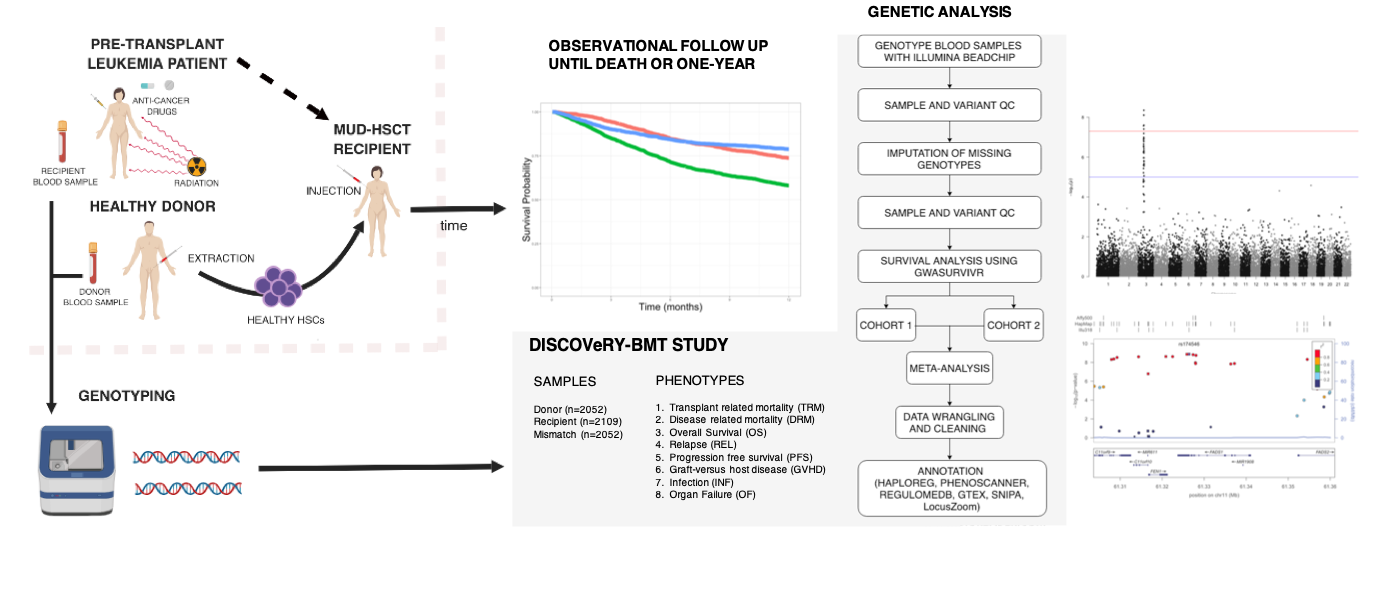
\includegraphics[width=8.7in, height=7.5in]{~/Desktop/figures/abstract/pipeline_draft.png}
    \caption[Graphical Abstract]{Graphical Abstract. The flow of the abstract begins on the upper left, illustrating the HSCT process of a patient receiving chemotherapy and/or radiation prior to kill all of the patients bone marrow cells prior to allogeneic HSCT. An HLA matched donor donates their healthy hematopoietic stem cells (HSCs) to the recipient. We genotyped both the donor and recipient blood samples for a GWAS testing for associations with survival outcomes. The gray boxes describe the DISCOVeRY-BMT phenotype and sample sizes, as well as our workflow pipeline. The graphical figures on the far right are typical output after GWAS (Manhattan plot and regional plot) to visualize results.}
    \label{fig:abstract}  
\end{figure}
\end{landscape}
}

\newpage

\pagestyle{plain} \fancyhead[L]{} \fancyhead[R]{}
\fancyfoot[C]{\thepage} \addcontentsline{toc}{section}{Dedication}

\vspace*{\fill}

\begin{center}
    \doublespacing
    This is dedicated to Ezgi, \\
    my parents, my siblings, and their families, \\
    for their endless love and support. \\
    And to my sweet little pooch Bernie.
  \end{center}

\vspace*{\fill}

\newpage

\pagestyle{plain} \fancyhead[L]{} \fancyhead[R]{}
\fancyfoot[C]{\thepage} \chapter*{ACKNOWLEDGEMENTS}
\addcontentsline{toc}{section}{Acknowledgments}

\doublespacing

I would like to express my deepest gratitude to my adviser Dr.~Lara
Sucheston-Campbell. She has been an incredible mentor for me and has set
me up with any and every opportunity that I have had my eyes on. She
really cares about her students and I am truly grateful for that.

I am forever indebted to my Master's adviser, Dr.~Barbara Foster, for
taking a chance on me and working her magic to get me an opportunity to
interview for a PhD position at RPCI. This was done despite the
application cycle closing several months beforehand, the incoming class
was full, and the next academic year was beginning in a matter of weeks.

Dr.~Martin Morgan exposed to me wealth of knowledge on R and would take
time out of his extremely busy schedule to work one-on-one with me.
Dr.~Moray Campbell set me up with a career defining opportunity where I
went to Europe for a year and began my journey of pursuing quantitative
biology. Dr.~Seb Battaglia, my Master's co-adivser, his training
contributed to my successes in graduate school.

And thank you to Ezgi Karaesmen, I truly believe I would not had the
level of success I have had for past four years if it were not for you.
Your love, your support, your intelligence, and your ability to
challenge me on my scientific ideas and my ability to think have been
instrumental towards my development as a scientist, I cannot thank you
enough.

This work was supported by National Institute of Health/National Heart,
Blood, and Lung Institute R01HL102278 and National Institute of
Health/National Cancer Institute R03CA188733. Support provided by Center
for Computational Research at University at Buffalo.

\newpage

\pagestyle{plain} \fancyhead[L]{} \fancyhead[R]{}
\fancyfoot[C]{\thepage} \chapter*{VITA}
\addcontentsline{toc}{section}{Vita} \singlespacing

\dateitem{2012}{B.S. Biology, SUNY Fredonia}
\dateitem{2015}{M.Sc. Integrated Systems Biology,\\
University of Luxembourg} \dateitem{2015}{M.S. Natural Sciences,\\
University at Buffalo}
\dateitem{2016-present}{Graduate Research Associate, \\ 
Department of Pharmaceutics,\\
The Ohio State University}

\begin{filecontents*}{bibcode.tex}
\bib{Rizvi2018}{article}{
Author = {Rizvi, Abbas A.},
Author = {Karaesmen, Ezgi},
Author = {Morgan, Martin},
Author = {Preus, Leah},
Author = {Wang, Junke},
Author = {Sovic, Michael},
Author = {Hahn, Theresa},
Author = {Sucheston-Campbell, Lara E.},
Journal = {Bioinformatics},
Month = {Nov},
Title = {gwasurvivr: an R package for genome wide survival analysis},
Year = {2018}}



\bib{Long2018}{article}{
Author = {Long, Mark D.},
Author = {Singh, Prashant K.},
Author = {Russell, James R.},
Author = {Llimos, Gerard},
Author = {Rosario, Spencer}, 
Author = {Rizvi, Abbas A.},
Author = {van den Berg, Patrick R.},
Author = {Kirk, Jason},
Author = {Sucheston-Campbell, Lara E.},
Author = {Smiraglia, Dominic J.},
Author = {Campbell, Moray},
Issn = {1476-5594},
Journal = {Oncogene},
Month = {Aug},
Title = {The miR-96 and RAR$\gamma$ signaling axis governs androgen signaling and prostate cancer progression},
Year = {2018}
}

\bib{LSC2018}{article}{

Author = {Sucheston-Campbell, Lara E.},
Author = {Clay-Gilmour, Alyssa I.},
Author = {Barlow, William E.},
Author = {Budd, G. Thomas},
Author = {Stram, Daniel O.},
Author = {Haiman, Christopher A.},
Author = {Sheng, Xin},
Author = {Yan, Li},
Author = {Zirpoli, Gary},
Author = {Yao, Song},
Author = {Jiang, Chen},
Author = {Kouros, Owzar},
Author = {Hershman, Dawn},
Author = {Albain, Kathy S.},
Author = {Hayes, Daniel F.},
Author = {Moore, Halle C.},
Author = {Hobday, Timothy J.},
Author = {Stewart, James A.},
Author = {Rizvi, Abbas A.},
Author = {Isaacs, Claudine},
Author = {Salim, Muhammad},
Author = {Gralow, Jule R.},
Author = {Hortobagyi, Gabriel N.},
Author = {Livingston, Robert B.},
Author = {Kroetz, Deanna L.},
Author = {Ambrosone, Christine B.},
Journal = {Pharmacogenetics and Genomics},
Month = {Feb},
Number = {2},
Pages = {49-55},
Title = {Genome-wide meta-analyses identifies novel taxane-induced peripheral neuropathy-associated loci},  
Volume = {28},
Year = {2018}
}


\bib{Karaesmen2017}{article}{
Author = {Karaesmen, Ezgi},
Author = {Rizvi, Abbas A.},
Author = {Preus, Leah M.},
Author = {McCarthy, Philip L.},
Author = {Pasquini, Marcelo C.},
Author = {Onel, Kenan},
Author = {Zhu, Xiaochun},
Author = {Spellman, Stephen},
Author = {Haiman, Christopher A.},
Author = {Stram, Daniel O.},
Author = {Loreall Pooler},
Author = {Xin Sheng},
Author = {Qianqian Zhu},
Author = {Li Yan},
Author = {Qian Liu},
Author = {Qiang Hu},
Author = {Amy Webb},
Author = {Guy Brock},
Author = {Alyssa I. Clay-Gilmour},
Author = {Sebastiano Battaglia},
Author = {David Tritchler},
Author = {Song Liu},
Author = {Theresa Hahn},
Author = {Lara E. Sucheston-Campbell},
Journal = {Blood},
Month = {Aug},
Number = {13},
Pages = {1585-1596},
Title = {Replication and validation of genetic polymorphisms associated with survival after allogeneic blood or marrow transplant},
Volume = {130},
Year = {2017}
}

\bib{clay2017}{article}{
Author = {Alyssa I. Clay-Gilmour},
Author = {Theresa Hahn},
Author = {Leah M. Preus},
Author = {Kenan Onel},
Author = {Andrew Skol},
Author = {Eric Hungate},
Author = {Qianqian Zhu},
Author = {Christopher A. Haiman},
Author = {Daniel O. Stram},
Author = {Loreall Pooler},
Author = {Xin Sheng},
Author = {Li Yan},
Author = {Qian Liu},
Author = {Qiang Hu},
Author = {Song Liu},
Author = {Sebastiano Battaglia},
Author = {Xiaochun Zhu},
Author = {AnneMarie W. Block},
Author = {Sheila N. J. Sait},
Author = {Ezgi Karaesmen}, 
Author = {Abbas A. Rizvi},
Author = {Daniel J. Weisdorf},
Author = {Christine B. Ambrosone},
Author = {David Tritchler},
Author = {Eva Ellinghaus},
Author = {David Ellinghaus},
Author = {Martin Stanulla},
Author = {Jacqueline Clavel},
Author = {Laurent Orsi},
Author = {Stephen Spellman},
Author = {Marcelo C. Pasquini},
Author = {Philip L. McCarthy},
Author = {Lara E. Sucheston-Campbell},
Journal = {Blood Advances},
Month = {September},
Number = {20},
Pages = {1717-1728},
Title = {Genetic association with B-cell acute lymphoblastic leukemia in allogeneic transplant patients differs by age and sex},
Volume = {1},
Year = {2017}

}


\bib{rizvi2015}{thesis}{
Author = {Abbas A. Rizvi},
Month = {August},
School = {University at Buffalo},
Title = {Reprogramming androgen receptor and lysine-specific demethylase 1 transcriptome in castration-resistant prostate cancer},
Year = {2015}

}

\bib{denies2014}{article}{
Author = {DeNies, Maxwell S.},
Author = {Johnson, Jordan},
Author = {Maliphol, Amanda B.},
Author = {Bruno, Michael},
Author = {Kim, Annabelle},
Author = {Rizvi, Abbas A.},
Author = {Rustici, Kevyn},
Author = {Medler, Scott},
Journal = {Physiological Reports},
Month = {Jan},
Number = {1},
Pages = {e00204},
Title = {Diet-induced obesity alters skeletal muscle fiber types of male but not female mice},
Volume = {2},
Year = {2014}
}

\end{filecontents*}

\begin{publist}
\begin{biblist}
\normalsize
\bib{Rizvi2018}{article}{
Author = {Rizvi, Abbas A.},
Author = {Karaesmen, Ezgi},
Author = {Morgan, Martin},
Author = {Preus, Leah},
Author = {Wang, Junke},
Author = {Sovic, Michael},
Author = {Hahn, Theresa},
Author = {Sucheston-Campbell, Lara E.},
Journal = {Bioinformatics},
Month = {Nov},
Title = {gwasurvivr: an R package for genome wide survival analysis},
Year = {2018}}



\bib{Long2018}{article}{
Author = {Long, Mark D.},
Author = {Singh, Prashant K.},
Author = {Russell, James R.},
Author = {Llimos, Gerard},
Author = {Rosario, Spencer},
Author = {Rizvi, Abbas A.},
Author = {van den Berg, Patrick R.},
Author = {Kirk, Jason},
Author = {Sucheston-Campbell, Lara E.},
Author = {Smiraglia, Dominic J.},
Author = {Campbell, Moray},
Issn = {1476-5594},
Journal = {Oncogene},
Month = {Aug},
Title = {The miR-96 and RAR$\gamma$ signaling axis governs androgen signaling and prostate cancer progression},
Year = {2018}
}

\bib{LSC2018}{article}{

Author = {Sucheston-Campbell, Lara E.},
Author = {Clay-Gilmour, Alyssa I.},
Author = {Barlow, William E.},
Author = {Budd, G. Thomas},
Author = {Stram, Daniel O.},
Author = {Haiman, Christopher A.},
Author = {Sheng, Xin},
Author = {Yan, Li},
Author = {Zirpoli, Gary},
Author = {Yao, Song},
Author = {Jiang, Chen},
Author = {Kouros, Owzar},
Author = {Hershman, Dawn},
Author = {Albain, Kathy S.},
Author = {Hayes, Daniel F.},
Author = {Moore, Halle C.},
Author = {Hobday, Timothy J.},
Author = {Stewart, James A.},
Author = {Rizvi, Abbas A.},
Author = {Isaacs, Claudine},
Author = {Salim, Muhammad},
Author = {Gralow, Jule R.},
Author = {Hortobagyi, Gabriel N.},
Author = {Livingston, Robert B.},
Author = {Kroetz, Deanna L.},
Author = {Ambrosone, Christine B.},
Journal = {Pharmacogenetics and Genomics},
Month = {Feb},
Number = {2},
Pages = {49-55},
Title = {Genome-wide meta-analyses identifies novel taxane-induced peripheral neuropathy-associated loci},
Volume = {28},
Year = {2018}
}


\bib{Karaesmen2017}{article}{
Author = {Karaesmen, Ezgi},
Author = {Rizvi, Abbas A.},
Author = {Preus, Leah M.},
Author = {McCarthy, Philip L.},
Author = {Pasquini, Marcelo C.},
Author = {Onel, Kenan},
Author = {Zhu, Xiaochun},
Author = {Spellman, Stephen},
Author = {Haiman, Christopher A.},
Author = {Stram, Daniel O.},
Author = {Loreall Pooler},
Author = {Xin Sheng},
Author = {Qianqian Zhu},
Author = {Li Yan},
Author = {Qian Liu},
Author = {Qiang Hu},
Author = {Amy Webb},
Author = {Guy Brock},
Author = {Alyssa I. Clay-Gilmour},
Author = {Sebastiano Battaglia},
Author = {David Tritchler},
Author = {Song Liu},
Author = {Theresa Hahn},
Author = {Lara E. Sucheston-Campbell},
Journal = {Blood},
Month = {Aug},
Number = {13},
Pages = {1585-1596},
Title = {Replication and validation of genetic polymorphisms associated with survival after allogeneic blood or marrow transplant},
Volume = {130},
Year = {2017}
}

\bib{clay2017}{article}{
Author = {Alyssa I. Clay-Gilmour},
Author = {Theresa Hahn},
Author = {Leah M. Preus},
Author = {Kenan Onel},
Author = {Andrew Skol},
Author = {Eric Hungate},
Author = {Qianqian Zhu},
Author = {Christopher A. Haiman},
Author = {Daniel O. Stram},
Author = {Loreall Pooler},
Author = {Xin Sheng},
Author = {Li Yan},
Author = {Qian Liu},
Author = {Qiang Hu},
Author = {Song Liu},
Author = {Sebastiano Battaglia},
Author = {Xiaochun Zhu},
Author = {AnneMarie W. Block},
Author = {Sheila N. J. Sait},
Author = {Ezgi Karaesmen},
Author = {Abbas A. Rizvi},
Author = {Daniel J. Weisdorf},
Author = {Christine B. Ambrosone},
Author = {David Tritchler},
Author = {Eva Ellinghaus},
Author = {David Ellinghaus},
Author = {Martin Stanulla},
Author = {Jacqueline Clavel},
Author = {Laurent Orsi},
Author = {Stephen Spellman},
Author = {Marcelo C. Pasquini},
Author = {Philip L. McCarthy},
Author = {Lara E. Sucheston-Campbell},
Journal = {Blood Advances},
Month = {September},
Number = {20},
Pages = {1717-1728},
Title = {Genetic association with B-cell acute lymphoblastic leukemia in allogeneic transplant patients differs by age and sex},
Volume = {1},
Year = {2017}

}


\bib{rizvi2015}{thesis}{
Author = {Abbas A. Rizvi},
Month = {August},
School = {University at Buffalo},
Title = {Reprogramming androgen receptor and lysine-specific demethylase 1 transcriptome in castration-resistant prostate cancer},
Year = {2015}

}

\bib{denies2014}{article}{
Author = {DeNies, Maxwell S.},
Author = {Johnson, Jordan},
Author = {Maliphol, Amanda B.},
Author = {Bruno, Michael},
Author = {Kim, Annabelle},
Author = {Rizvi, Abbas A.},
Author = {Rustici, Kevyn},
Author = {Medler, Scott},
Journal = {Physiological Reports},
Month = {Jan},
Number = {1},
Pages = {e00204},
Title = {Diet-induced obesity alters skeletal muscle fiber types of male but not female mice},
Volume = {2},
Year = {2014}
}


\end{biblist}
\end{publist}

\begin{fieldsstudy}
\majorfield*
\end{fieldsstudy}

\newpage

\pagestyle{plain} \fancyhead[L]{} \fancyhead[R]{}
\fancyfoot[C]{\thepage} \tableofcontents

\newpage

\pagestyle{plain} \fancyhead[L]{} \fancyhead[R]{}
\fancyfoot[C]{\thepage} \listoftables

\newpage

\pagestyle{plain} \fancyhead[L]{} \fancyhead[R]{}
\fancyfoot[C]{\thepage} \listoffigures

\newpage

\pagenumbering{arabic}

\newpage

\pagestyle{plain} \fancyhead[L]{} \fancyhead[R]{}
\fancyfoot[C]{\thepage} \chapter{Introduction} \doublespacing

Broadly, this dissertation examines the role of germline genetic
variation and survival outcomes in the matched unrelated donor (MUD)
hematopoietic stem cell transplantation (HSCT) patients with acute
myeloid leukemia (AML), acute lymphoblastic leukemia (ALL), or
myelodysplastic syndrome (MDS) who received HSCT as curative therapy. In
addition, this dissertation also seeks to enhance the computational
workflows that are used in to identify genetic variants associated with
worse (or better survival) after HSCT. The significance is three-fold,
first, we can identify clinically relevant markers that may improve
donor selection beyond traditional methods; second, we can characterize
pre-transplant risk of disease or transplant related death within the
first year; and third, we can help facilitate other researchers studying
similar problems with similar data or data structures by developing
open-source software. Six chapters comprise my dissertation. Chapter 1
first introduces genetic association studies, allogeneic HSCT and
DISCOVeRY-BMT genome wide-association study (GWAS), including the
corresponding clinical data in detail. Chapter 2 will discuss a
replication and validation of genetic variants shown to be significantly
associated with survival outcomes after transplant; this work is has
been published. Chapter 3 discusses in detail the R package that we
developed to perform genome wide survival analyses; this work has been
published and the package freely available. Chapter 4 is the application
of the R package and custom pipeline developed to perform large
automated GWAS, specialized to our lab, but importantly generalizable in
a broader (and larger context). Chapter 5 discusses the discovery and
inference of markers of survival in ALL donor and recipient following
transplant. This dissertation ends with Chapter 6, which briefly reviews
the contents of this dissertation, discusses ongoing research in our
laboratory and the future directions that should be undertaken.

\section{Genetic Association Studies}\label{genetic-association-studies}

Genetic association studies test for correlations between genetic
variation as it relates to disease risk or to physical quantitative
traits (i.e.~height or weight) (C. M. Lewis and Knight
\protect\hyperlink{ref-Lewis_2012}{2012}). These studies have been
successful in identifying variants associated disease susceptibility or
drug response and have helped us understand that many diseases have
complex genetic signatures that need to be further understood (Visscher
et al. \protect\hyperlink{ref-Visscher_2012}{2012}). The human genome
consists of over 3 billion base pairs, all of which are contained in
every nucleated cell in the body. A genome sequence is the complete
collection of all nucleotides (A, C, T, or G for DNA genomes) that make
up all the chromosomes in individuals or species (Lan- der et al. 2001).
The vast majority of nucleotides (\textgreater{}99.5\%) are identical
between individuals within a species, however, genetic variation arises
within individuals and populations over time and different spaces.
Indeed, the fundamental source of genetic variation is mutation, where
permanent alterations occur to a single nucleotide or larger structural
changes in the genome of a species. A variant at single position (locus)
in a DNA sequence that occurs in at least 1\% of a population is called
a single nucleotide polymorphism (SNP). SNPs are the most widely used
marker to describe genetic variation. Larger structural variations may
include microsatellite regions, insertion/deletions (indels), copy
number variations (CNVs), or variable-tandem repeats (VNTRs) all of
which have importance in understanding the genetic architecture and
disease etiology (Sudmant et al.
\protect\hyperlink{ref-Sudmant_2015}{2015}). For purposes of this
document, unless otherwise specified, genetic variation will refer to
single nucleotide polymorphisms (SNPs). SNPs will also be referred to as
simply as polhmorphisms, genetic markers, or markers interchangeably.

Different forms of the same variant are called alleles. For diploid
organisms,one allele is passed from each parent. At a given locus in the
genome, individuals can have two copies of the same allele (called
homozygous) or two different copies of alleles (heterozygous). Sequence
variations can occur coding regions of genes, non-coding regions of
genes, or intergenic regions (between genes). SNPs in coding regions are
synonymous, meaning the amino acid sequences are the same and therefore
do not change protein structure, or non-synonymous SNPs, the change in
basepair changes the amino acid sequence. Non-synonymous SNPs are
further stratified into two types: missense SNPs, which result in codon
changes that code for different amino acids (Z. Shi and Moult
\protect\hyperlink{ref-shi_2011}{2011}) and nonsense SNPs, which result
in a premature stop codon that often yield a non-functional or truncated
protein product. Most polymorphisms are in non-coding regions, however
despite the fact there is not an immediately obvious consequence they
may alter important transcriptional properties such as gene splicing,
transcription factor binding, or messenger RNA (mRNA) decay (Green et
al. \protect\hyperlink{ref-green_2003}{2003}). SNPs may affect gene
expression (and may be upstream or downstream from a gene) are called
expression quantiative trait loci (eQTL).

Over the past two decades, research has increasingly evolved from
looking at specific regions of interest (candidate gene association
studies) to more agnostic approaches that investigate larger portions of
the genome, such as genome wide association studies (GWAS), whole-exome
sequencing studies (WES studies) and whole-genome sequencing studies
(WGS studies) (Timpson et al.
\protect\hyperlink{ref-Timpson_2018}{2018}). This dissertation is
primarily focused on GWAS, specifically the application of using GWAS in
the context of identifying common variants in after hematopoietic stem
cell transplantation (HSCT), where more details will be discussed in
subsequent subsections of this chapter.

GWAS employ genotyping microarrays to measure genetic variation -- and
they have become the standard platform in academic and industry to test
for association of phenotype with common genetic variants. Common
genetic variants are defined as those with a \emph{minor allele
frequency} (MAF) of \(\geq\) 1\% and rare variants are defined as those
with a MAF \(\leq\) than 1\%. Genotyping microarrays are designed to
contain common variants but optionally can contain rare variants. GWAS
ask if the allele of a genetic variant is found more often than what
would be expected than by random chance in individuals with the
phenotype of interest (e.g.~the disease being studied). If the variant
(one allele) occurs more in those affected by the disease than those
without the disease, then the variant deemed as being \emph{associated}
with the disease. Nonetheless, GWAS have been very successful at
revealing new pathways involved in disease, but often the post-GWAS
understanding of the associations is poorly understood. That is,
identification of causal variants, biological relevance and the
interaction that these associations have with other genetic or
environmental factors.

\subsection{Linkage Disequilibrium}\label{linkage-disequilibrium}

GWAS are heavily based on the principal of linkage disequilibrium (LD)
at the population level. LD is the non-random dependence of allele
frequencies at two more loci in the general population (Jorde
\protect\hyperlink{ref-Jorde_2000}{2000}). LD reflects the relationship
between alleles at different loci. In other words, LD is a measure of
two alleles or specific sequences being inherited together. The unit of
measure for LD is \(r^{2}\) (squared correlation coefficient) (J. K.
Pritchard and Przeworski \protect\hyperlink{ref-Pritchard_2001}{2001}).
In general, loci that are in close proximity exhibit stronger LD (J. K.
Pritchard and Przeworski \protect\hyperlink{ref-Pritchard_2001}{2001}).
Perfect LD (\(r^{2}\) = 1) means that no recombination occurred on this
chunk of genome. Regions that are further apart on a chromosome exhibit
weaker LD (D. E. Reich et al. \protect\hyperlink{ref-Reich_2001}{2001}).
Low LD means that recombination occurred and that there are lots of
possible rearrangements that may have occurred during meiosis. LD decay
influences the number of SNPs needed to ``tag'' a haplotype, and that
number of SNPs is just a small subset of the number of segregating
polymorphisms in the population (D. E. Reich et al.
\protect\hyperlink{ref-Reich_2001}{2001}). Knowledge of haplotype
structure makes it possible to retrieve more information from GWAS.
Tagging SNPs with known haplotype block structure can capture much of
the genetic information in a region.

With the rapid growth of genetic association studies and statistical
methods assessing genetic variation, researchers routinely exploit LD to
map regions in the human genome. While costs of genotyping have lowered
over the past decade, a major barrier to overcome when conducting large
scale studies, was the expense of searching the entire genome for
disease associations (International HapMap Consortium
\protect\hyperlink{ref-hapmap_2005}{2005}). The International HapMap
Project (International HapMap Consortium
\protect\hyperlink{ref-hapmap_2005}{2005}) was the first attempt to
address these challenges. HapMap was a large scale multi-institutional
international project that finely mapped common genetic variation (or
establish a ``haplotype map''). HapMap demonstrated that genomic blocks
are shared in common areas across continental population. HapMap
alleviated high costs of studies by preferentially selecting `tag' SNPs
that covered the entire genome, and due to LD structure, inference could
be drawn about nearby variants that were not genotyped (Bakker et al.
\protect\hyperlink{ref-bakker_2005}{2005}). HapMap ended with a
catalogue across several populations for 420 haplotypes at 3.5 million
SNPs(International HapMap Consortium et al.
\protect\hyperlink{ref-hapmap_2007}{2007}). Afterwards, the 1000 Genomes
Project, with similar ambitions to HapMap, aimed to create a more
complete and thorough catalogue of human genetic variation, which could
be leveraged for GWAS investigating disease (1000 Genomes Project
Consortium \protect\hyperlink{ref-1000genomes}{2015}). The consortium
aimed to discover \textgreater{}95\% of variants with MAF as low as 1\%
across the genome, as well as estimate population specific allele
frequencies, haplotype maps and LD patterns of alleles (1000 Genomes
Project Consortium et al. \protect\hyperlink{ref-1kb_phase1}{2010}). The
results provided a more comprehensive picture of human genetic variation
than what was previously available (5,008 haplotypes at over 88 million
SNPs in 26 worldwide populations) (1000 Genomes Project Consortium et
al. \protect\hyperlink{ref-1kb_phase1}{2010}). And even more recently,
the Haplotype Reference Consortium (HRC) has described nearly 65,000
human haplotypes at \textasciitilde{}40 million SNPs via whole-gene
sequence data from predominantly European ancestry (McCarthy et al.
\protect\hyperlink{ref-hrc}{2016}). Other reference panels have been
developed, particularly population specific ones, but are beyond the
scope of this document.

\subsection{Genetic Imputation}\label{genetic-imputation}

Genetic imputation (will also be simply referred to as imputation) has
had significant contributions to genetic association studies. Imputation
can be defined as predicting unobserved genotypes that were not directly
assayed in a sample of individuals. The term refers to when a reference
panel of haplotypes at set of a SNPs is used to impute SNPs that have
been genotyped at a subset of that set of SNPs (Marchini et al.
\protect\hyperlink{ref-snptest}{2007}). Genotype imputation is useful
for three reasons: (1) by boosting the number of SNPS that can be tested
for association, thus increasing the power of the study, (2) homogenizes
variant sets for meta-analyses, and (3) help control false positive for
which genotype calling is challenging (Marchini and Howie
\protect\hyperlink{ref-marchini_impute}{2010}).

Today, several reference panels are available, such as (but not limited
to) HapMap2 (International HapMap Consortium
\protect\hyperlink{ref-hapmap_2005}{2005}), 1000 Genomes Phase 3 (1000
Genomes Project Consortium \protect\hyperlink{ref-1000genomes}{2015}),
HRC (McCarthy et al. \protect\hyperlink{ref-hrc}{2016}), which differ by
the number of samples, sites (chromosomes 1-22, X), and number of
haplotypes. These reference panels are widely used to carry out accurate
imputation in studies. HRC can impute SNPs with MAF as low as 0.1\%
(McCarthy et al. \protect\hyperlink{ref-hrc}{2016}). Most studies take a
two step approach that first will impute the missing genotypes using the
reference panel without consideration of the phenotype. The imputed
genotypes are then tested for association with the phenotype in the
second pass. Multiple phenotypes can be tested for association without
the need for re-imputation.

Several imputation algorithms and software packages are available as
stand-alone software, such as IMPUTE2 (B. N. Howie, Donnelly, and
Marchini \protect\hyperlink{ref-Howie_2009}{2009}), MaCH (Li et al.
\protect\hyperlink{ref-mach_2010}{2010}), BEAGLE (B. L. Browning and
Browning \protect\hyperlink{ref-browning_2016}{2016}) or from imputation
web services, such as the Sanger imputation server (McCarthy et al.
\protect\hyperlink{ref-hrc}{2016}, R. Durbin
(\protect\hyperlink{ref-durbin_2014}{2014})) or the University of
Michigan imputation server (Das et al.
\protect\hyperlink{ref-michigan_imputation}{2016}). The details of the
imputation methods are beyond the scope of this dissertation, but very
briefly, each algorithm is an extension of the hidden Markov model
(HMMs) to carry out inference when modeling LD or haplotype estimation
(also called phasing; N. Li and Stephens
(\protect\hyperlink{ref-li_2003}{2003})). The imputation methods vary in
terms slight methodological differences in estimating haplotypes,
computational performance and error rates.

\subsection{Meta-analysis}\label{meta-analysis}

Although GWAS have been successful at identifying novel loci that are
associated to some disease or trait, the finding typically have modest
effects and large sample sizes are needed to detect common variants with
small effect sizes. In order to improve the power to detect variants
with small effect sizes, meta-analyses have been used. Meta-analysis
using summary statistics has been important for GWAS of complex genetic
diseases and traits (Bakker et al.
\protect\hyperlink{ref-bakker_2008}{2008}). Researchers combine the
effects of multiple studies without having to integrate both genotype
and phenotype data. After imputation, meta-analysis is useful for
different cohorts that are used on different genotyping chips to boost
power.

A popular tool to perform meta-analysis on GWAS is METAL (Willer, Li,
and Abecasis \protect\hyperlink{ref-metal}{2010}). METAL can combine
either test statistics and standard errors, or p-values across studies
(while taking direction of effect and sample size into account). The
results are combined using fixed-effects or random-effects models.

\section{Hematopoietic Stem Cell
Transplantation}\label{hematopoietic-stem-cell-transplantation}

Blood cells continuously go through a self-renewing maturation process
from less differentiated precursor cells to mature cells in a process
called hematopoiesis (Copelan
\protect\hyperlink{ref-copelan_2006}{2006}). The process begins with
hematopoietic stem cells (HSCs) which are located in center of bone
marrow. HSCs differentiate into either lymphoid or myeloid progenitor
cells and further develop into one of three lineages: red blood cells
(erythrocytes), lymphocytes (T-cells, B-cells, and natural killer (NK)
cells), and myeloid cells (granulocytes, megakaryocytes, and
macrophages). All of these blood cells have vital roles in the human
body. Tumors arise from malignant stem cells that usually originate from
normal stem cells but retain the self-renewal property. Leukemic cells
are limited in their ability to proliferate and incessantly are
replenished from leukemic stem cells. Acute leukemias are characterized
by the rapid increase of immature blood cells, such that the bone marrow
is unable to produce healthy blood cells. Immediate treatment is
required. Acute leukemias can be treated with some combination of
chemotherapy, radiation therapy or an HSCT. When all other treatment
options have been exhausted, an HSCT is used as last resort.

HSCT is an established therapeutic procedure that is used as a
potentially curative treatment for life-threatening congenital or
acquired blood disorders (malignant or non-malignant) (Henig and
Zuckerman \protect\hyperlink{ref-Henig_2014}{2014}). HSCT involves the
intravenous infusion of autologous or allogeneic hematopoietic
progenitor cells to restore normal function in patients whose bone
marrow is compromised. Autologous HSCT involves self-donation of marrow
stem cells, whereas allogeneic HSCT is when stem cells are transferred
from a HLA-matched related donor (MRD) or a HLA-matched unrelated donor
(MUD). Although a matched sibling donor is preferred, only approximately
30\% of patients who may benefit from HSCT have such a donor available.
In the United States, the number of allogeneic transplants yearly has
dramatically risen over the past decade, across all diseases (M.
Pasquini et al. \protect\hyperlink{ref-Pasquini_2013}{2013}). Patients
with acute myeloid leukemia (AML), acute lymphoblastic leukemia (ALL),
or myelodysplastic syndrome (MDS), represent the largest group treated
with allogeneic HSCT. While both patient care and matching has improved
over the past few decades almost half of all high-resolution 10/10 HLA
MUD-HSCT recipients die within one-year post-transplant due to either
their disease or transplant-related causes (M. Pasquini et al.
\protect\hyperlink{ref-Pasquini_2013}{2013}). These trends also show
transplant-related causes are a larger contributor to mortality within
the first 100-days post-transplant and shift towards primary disease
after approximately six months post-transplant (D'Souza et al.
\protect\hyperlink{ref-DSouza_2017}{2017}). Reducing TRM without
increasing risk of disease death and vice versa continue to represent a
substantial clinical challenge.

\noindent The four elements of HSCT are:

\noindent 1. Graft Source\\
The graft sources are either from bone marrow or peripheral blood stem
cells (PBSCs). For bone marrow grafts, hematopoietic stem cells (HSCs)
are typically extracted from the center of the posterior iliac crest
(pelvis) using a large needle while the donor is under general
anesthesia (Copelan \protect\hyperlink{ref-copelan_2006}{2006}). HSCs
are continually going through a cycle of detaching from the bone marrow
and entering circulation and back into the bone marrow, making it very
convenient to use the peripheral blood as a source.

\noindent 2. Graft Type\\
The graft can either be autologous, syngeneic, allogeneic, or from
umbilical cord blood. Autologous HSCTs are self-donating, where a
patient's marrow is taken and treated exogeneously. In that time the
patient is treated with chemotherapy to reduce the tumor burden and then
cells are donated back to the patient. Syngeneic transplants are when
the donor is an identical twin. And allogeneic HSCTs are when a related
or unrelated donor is the graft source. Umbilical cord blood transplants
are rich in HSCs but limited in volume and are less common than the
other forms of transplant.

\noindent 3. HLA matching\\
HLA genes are closely linked on chromosome 6 and are inherited as
haplotypes. HLA encodes for the major histocompatibility complex (MHC).
MHC are class of molecules that are found on antigen presenting cells
and are important for imitating immune response. MHC has two primary
classes, class I and class I. MHC class I is encoded by HLA-A, -B, and
-C. MHC class II is encoded by HLA-DP, -DM, -DOA, -DOB, -DQ, and -DR.
The preferred HLA match for an allogeneic donor is high resolution typed
10/10, which means the matched alleles are at HLA-A, -B, -C, -DQ, and
-DP. Survival varies considerably depending on which HLA alleles are
matched. A single mismatch is a significant risk factor for development
of GVHD and is associated with higher mortality and decreased survival
(Hamilton and Copelan \protect\hyperlink{ref-hamilton_2012}{2012}).

\noindent 4. Pre-transplant conditioning regimens\\
Patients are given pre-transplant chemotherapy to reduce tumor burden of
the leukemia. HSCTs are most successful when patients are in first
complete remission (CR1). These can include myeloablative chemotherapy
or reduce intensity therapy.

\section{DISCOVeRY-BMT}\label{discovery-bmt}

\underline{D}etermining the \underline{I}nfluence of
\underline{S}usceptibility \underline{CO}nveying \underline{V}ariants
\underline{R}elated to one-\underline{Y}ear mortality after
\underline{B}one \underline{M}arrow \underline{T}ransplant
(DISCOVeRY-BMT) is a GWAS. This GWAS aims at identifying and
characterizing non-human leukocyte antigen (HLA) genetic variation in
the context of survival outcomes in acute lymphoblastic leukemia (ALL),
acute myelogenous leukemia (AML) and myelodysplastic syndrome (MDS)
patients and their matched unrelated donor (MUD) after hematopoietic
stem cell transplantation (HSCT) (L. E. Sucheston-Campbell et al.
\protect\hyperlink{ref-lsc_2015}{2015}). HSCT is also called bone marrow
transplantation (BMT) and hence both terms will be used interchangeably
throughout this document. Additionally, the terms recipients and
patients will be used interchangeably.

\subsection{Patient Characteristics}\label{patient-characteristics}

DISCOVeRY-BMT investigates donor and recipient genetic factors that
contribute to 1 year cause-specific mortality after MUD-HSCT (Hahn et
al. \protect\hyperlink{ref-Hahn_2015}{2015}; L. E. Sucheston-Campbell et
al. \protect\hyperlink{ref-lsc_2015}{2015}; Clay-Gilmour et al.
\protect\hyperlink{ref-Clay_2017}{2017}). This GWAS comprises two
independent cohorts. All patients in DISCOVeRY-BMT were reported to the
Center for International Blood and Marrow Research (CIBMTR) and had
banked biorepository samples (blood samples) from recipients and donors
at the National Marrow Donor Program (NMDP). Data that were reported to
CIBMTR was collected from 151 transplant centers in the USA.
Furthermore, all patients were de-identified and approved by the Roswell
Park Cancer Institute Institutional Review Board and signed informed
consent for research. Although no patients were excluded based on
gender, age, or race, over 90\% of DISCOVeRY-BMT cohorts were of
self-reported European American ancestry. Additional exclusion criteria
included: umbilical cord blood graft, \emph{ex vivo} T-cell depleted
graft or the patient underwent a prior autologous or allogeneic
transplant.

Blood samples were genotyped and comprise the genotype data is the
``genetic data'' that is reported throughout this dissertation. In
preparation for this GWAS, all post-mortem cause-specific deaths of the
patients were reviewed and judged by a post-mortem by an expert panel
(Hahn et al. \protect\hyperlink{ref-Hahn_2015}{2015}). The review and
adjudicated of cause of death was conducted because many of the 151
centers the data are inconsistent in reporting and classification of
outcome attributions. Thus the panel was established for concordance in
cause of death, logic, and quality. Re-assessment by the panel was
performed using autopsy reports and death certificates. The panel
consisted of three HSCT oncologists and a HSCT clinical epidemiologist
(Hahn et al. \protect\hyperlink{ref-Hahn_2015}{2015}).

\rowcolors{2}{gray!6}{white}

\begin{table}[t]

\caption{\label{tab:unnamed-chunk-12}\label{tab:dbmt_cohorts} Donor and Recipients Disease Proportions by Cohort in DISCOVeRY-BMT.}
\centering
\fontsize{9}{11}\selectfont
\begin{threeparttable}
\begin{tabular}{lllll}
\hiderowcolors
\toprule
\multicolumn{1}{c}{ } & \multicolumn{2}{c}{Donor (N/Percent \%)} & \multicolumn{2}{c}{Recipient (N/Percent \%)} \\
\cmidrule(l{3pt}r{3pt}){2-3} \cmidrule(l{3pt}r{3pt}){4-5}
  & Cohort 1 & Cohort 2 & cohort 1 & cohort 2\\
\midrule
\showrowcolors
ALL & 468 (23\%) & 93 (12\%) & 483 (23\%) & 94 (12\%)\\
AML & 1247 (61\%) & 478 (63\%) & 1282 (61\%) & 488 (63\%)\\
MDS & 337 (16\%) & 192 (25\%) & 345 (16\%) & 195 (25\%)\\
\hline
Total & 2052 & 763 & 2110 & 777\\
\bottomrule
\end{tabular}
\begin{tablenotes}[para]
\item Shown here are disease proportions of ALL, AML and MDS in DISCOVeRY-BMT cohorts. The percentage in each cell is computed column-wise as the proportion of sample size (N) within a cohort across disease group.
\end{tablenotes}
\end{threeparttable}
\end{table}

\rowcolors{2}{white}{white}

Both cohorts comprise AML, ALL, or MDS patients who were T-cell replete
and treated with myeloablative (MA) or reduced intensity (RIC)
conditioning regimens prior to transplant. Cohort 1 included 2110 HSCT
recipients and 2052 10/10 HLA matched unrelated donors (matched at
HLA-A, -B, -C, -DRB1, and -DQB1) from 2000 to 2008 (Table
\ref{tab:dbmt_cohorts}). Cohort 2 included 763 donors and 777 recipients
from the years 2000 to 2011 (Table \ref{tab:dbmt_cohorts}). A subset of
patients (\(N=281\)) in cohort 2 were 8/8 HLA matched (matched at HLA-A,
-B, -C, -DRB1), while the remaining patients (n=496) had the same
matching criteria as Cohort 1 and are 10/10 HLA matched.

The proportion of patients with AML is relatively consistent between
cohorts at approximately 60\% of patients (Table
\ref{tab:dbmt_cohorts}). However, the proportion of ALL and MDS patients
shifts between cohorts. For ALL, in cohort 1 the proportion is 23\%,
while in cohort 2, the proportion is 12\% (Table
\ref{tab:dbmt_cohorts}). Similarly, for MDS, in cohort 1 the proportion
of patients with this disease is 16\% and in cohort 2 it is 25\% (Table
\ref{tab:dbmt_cohorts}). For all future analyses in this dissertation,
MDS is never analyzed alone. MDS is either analyzed with ALL and AML
(AML + ALL + MDS), or with AML (AML + MDS).

\subsection{Survival Outcome
Definitions}\label{survival-outcome-definitions}

\rowcolors{2}{gray!6}{white}

\begin{table}[t]

\caption{\label{tab:unnamed-chunk-13}\label{tab:dbmt_outcomes} Definitions of Survival Outcomes}
\centering
\fontsize{9}{11}\selectfont
\begin{tabular}{l>{\raggedright\arraybackslash}p{16em}}
\hiderowcolors
\toprule
Outcomes & Definitions\\
\midrule
\showrowcolors
Overall Survival (OS) & defined as any patient (recipient) that died at any point within the first 12 month window post-HSCT of this observational study.\\
Transplant Related Mortality (TRM) & defined as any cause of death except the underlying disease, pre-existing disease, accidental death or suicide, or death unrelated to the transplant.\\
Disease Related Mortality (DRM) & broadly defined as deaths relating to leukemia/MDS relapse/progression, including death attributed to toxicity or infection from anti-leukemic treatments post-HSCT.\\
Progression Free Survival (PFS) & is defined as the time to relapse. All patients were analyzed as time to progression of disease\\
Relapse (REL) & patients who were not in CR pre-HSCT and the disease returns (relapse) after HSCT.\\
\bottomrule
\end{tabular}
\end{table}

\rowcolors{2}{white}{white}

The survival outcomes are cause-specific deaths during the first year
post-HSCT that were reviewed and re-assessed with high confidence
(described above). The survival outcomes included are: overall survival
(OS), disease related mortality (DRM), and transplant related mortality
(TRM), progression-free survival (PFS) and relapse (REL) (Table
\ref{tab:dbmt_outcomes}).

TRM subtypes were further stratified into graft-versus-host disease
(GVHD), organ failure (OF), infection (INF), or other. Other causes of
death included more rare events, such as (but not limited to) secondary
malignancies, primary or secondary graft failure, or hemorrhage. Despite
being adjudicated, TRM subtypes are difficult to differentiate from one
another, and some times more than one may present in the autopsy or
report. The boundaries aren't necessarily clear so there may be overlap
between these patients. Nevertheless, GVHD deaths included acute or
chronic GVHD, conditional upon a patient actively receiving treatment
for GVHD at the time of death. Deaths that were considered to be
infection were identified as arising from bacterial, fungal, viral,
and/or protozoan organisms that caused organ damage. OF deaths were
defined as organ toxicity relating to the transplant and not due to
disease progression, GVHD, or infection.

The phenotypes that are tested in DISCOVeRY-BMT are stratified into
different disease groups:\\
1. Mixed Disease -- which includes AML, MDS, and ALL (the full
cohort).\\
2. AML + MDS -- the myeloid malignancies being grouped together,
excluded the lymphoid lineage (ALL)\\
3. AML only -- includes only AML\\
4. ALL only -- includes only ALL\\
5. MDS only -- includes only MDS. This will not be tested or discussed
in much detail.

\rowcolors{2}{gray!6}{white}

\begin{table}[t]

\caption{\label{tab:unnamed-chunk-14}\label{tab:dbmt_props} Proportion of Events by Survival Outcome}
\centering
\fontsize{9}{11}\selectfont
\begin{tabular}{lll}
\hiderowcolors
\toprule
\multicolumn{1}{c}{ } & \multicolumn{2}{c}{Recipient (N/Percent \%)} \\
\cmidrule(l{3pt}r{3pt}){2-3}
Outcome & Cohort 1 & Cohort 2\\
\midrule
\showrowcolors
\addlinespace[.5em]
\multicolumn{3}{l}{\textbf{Mixed Disease}}\\
\hspace{1em}Disease related mortality (DRM) & 474 (22.46\%) & 168 (21.62\%)\\
\hspace{1em}Transplant related mortality (TRM) & 405 (19.19\%) & 141 (18.15\%)\\
\hspace{1em}Overall survival (OS) & 879 (41.66\%) & 309 (39.77\%)\\
\hspace{1em}Relapse (REL) & 639 (30.28\%) & 233 (29.99\%)\\
\hspace{1em}Progression free survival (PFS) & 1055 (50\%) & 374 (48.13\%)\\
\hspace{1em}Graft-versus-host disease (GVHD) & 134 (6.35\%) & 59 (7.59\%)\\
\hspace{1em}Infection (INF) & 122 (5.78\%) & 36 (4.63\%)\\
\hspace{1em}Organ failure (OF) & 104 (4.93\%) & 26 (3.35\%)\\
\addlinespace[.5em]
\multicolumn{3}{l}{\textbf{AML + MDS }}\\
\hspace{1em}Disease related mortality (DRM) & 383 (23.54\%) & 149 (21.82\%)\\
\hspace{1em}Transplant related mortality (TRM) & 297 (18.25\%) & 121 (17.72\%)\\
\hspace{1em}Overall survival (OS) & 680 (41.79\%) & 270 (39.53\%)\\
\hspace{1em}Relapse (REL) & 506 (31.1\%) & 208 (30.45\%)\\
\hspace{1em}Progression free survival (PFS) & 810 (49.78\%) & 329 (48.17\%)\\
\hspace{1em}Graft-versus-host disease (GVHD) & 97 (5.96\%) & 55 (8.05\%)\\
\hspace{1em}Infection (INF) & 90 (5.53\%) & 27 (3.95\%)\\
\hspace{1em}Organ failure (OF) & 76 (4.67\%) & 21 (3.07\%)\\
\addlinespace[.5em]
\multicolumn{3}{l}{\textbf{AML Only}}\\
\hspace{1em}Disease related mortality (DRM) & 333 (25.98\%) & 115 (23.57\%)\\
\hspace{1em}Transplant related mortality (TRM) & 211 (16.46\%) & 73 (14.96\%)\\
\hspace{1em}Overall survival (OS) & 544 (42.43\%) & 188 (38.52\%)\\
\hspace{1em}Relapse (REL) & 431 (33.62\%) & 161 (32.99\%)\\
\hspace{1em}Progression free survival (PFS) & 648 (50.55\%) & 234 (47.95\%)\\
\hspace{1em}Graft-versus-host disease (GVHD) & 61 (4.76\%) & 26 (5.33\%)\\
\hspace{1em}Infection (INF) & 69 (5.38\%) & 14 (2.87\%)\\
\hspace{1em}Organ failure (OF) & 59 (4.6\%) & 18 (3.69\%)\\
\addlinespace[.5em]
\multicolumn{3}{l}{\textbf{ALL Only}}\\
\hspace{1em}Disease related mortality (DRM) & 91 (18.84\%) & 19 (20.21\%)\\
\hspace{1em}Transplant related mortality (TRM) & 108 (22.36\%) & 20 (21.28\%)\\
\hspace{1em}Overall survival (OS) & 199 (41.2\%) & 39 (41.49\%)\\
\hspace{1em}Relapse (REL) & 133 (27.54\%) & 25 (26.6\%)\\
\hspace{1em}Progression free survival (PFS) & 245 (50.72\%) & 45 (47.87\%)\\
\hspace{1em}Graft-versus-host disease (GVHD) & 37 (7.66\%) & 4 (4.26\%)\\
\hspace{1em}Infection (INF) & 32 (6.63\%) & 9 (9.57\%)\\
\hspace{1em}Organ failure (OF) & 28 (5.8\%) & 5 (5.32\%)\\
\bottomrule
\end{tabular}
\end{table}

\rowcolors{2}{white}{white}

\begin{figure}

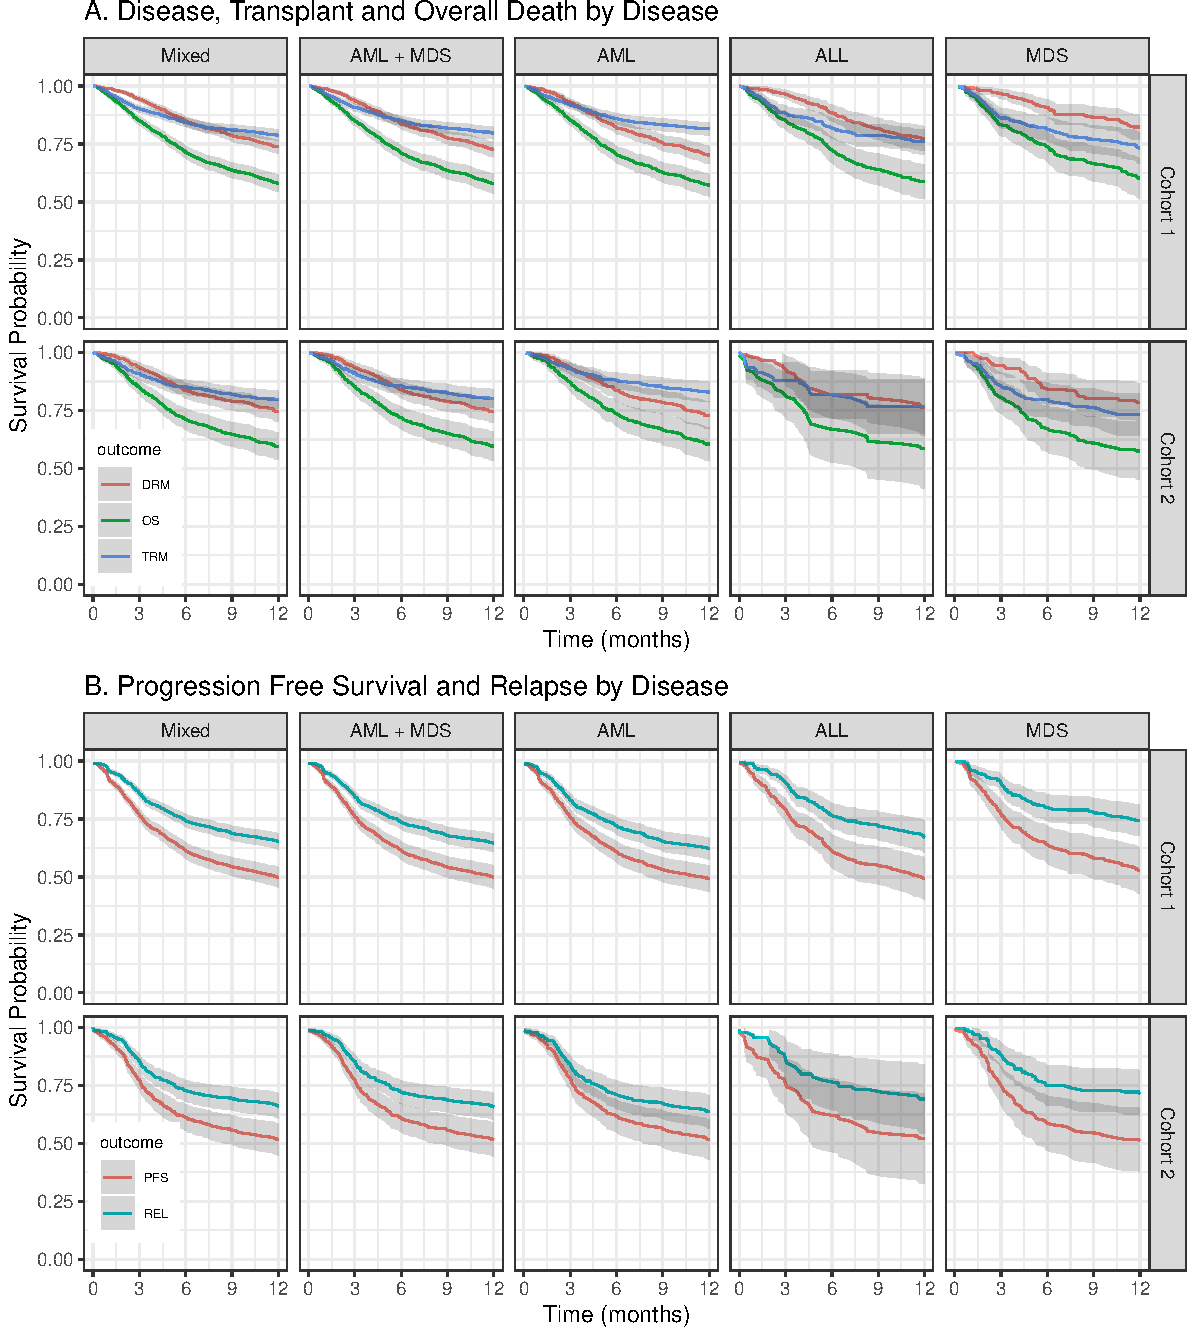
\includegraphics{figures/unnamed-chunk-15-1} \hfill{}

\caption{\label{fig:surv_curvs_outcome_disease} Survival curves for all disease groups being tested (Mixed disease, AML+MDS, AML only, and ALL only). The x-axis is survival probability. The y-axis is time in months. Cohorts 1 and 2 are shown in the left and right panel respectively. The gray shaded areas are 95 percent confidence intervals. (A) Red is disease-related mortality (DRM), green is overall survival (OS), and blue is transplant related mortality (TRM). (B) Cyan is relapse and red is progression free survival (PFS)}\label{fig:unnamed-chunk-15}
\end{figure}

In agreement with published CIBMTR statistics, about 40\% of patients
die after 1 year in both DISCOVeRY-BMT cohorts (Table
\ref{tab:dbmt_props}, Figure \ref{fig:surv_curvs_outcome_disease}).
Patients dying from transplant related causes is about 22\% between both
DISCOVeRY-BMT cohorts (Table \ref{tab:dbmt_props}). Similarly, about
18-19\% of patients die of their disease within the first year after
transplant (Table \ref{tab:dbmt_props}). Dying due to disease is the
leading cause of death in AML + MDS and AML only as well. Conversely,
for ALL, transplant related mortality is a larger contributor to overall
death than the other subgroups. Progression free survival is about 50\%
for the full cohort and disease subsets. AML alone has the most relapse
compared to all other groups.

Most TRM events happen early and then DRM supersedes TRM as the year
progresses (after about 6 months) for all diseases and myeloid subtypes
(Figure \ref{fig:surv_curvs_outcome_disease}A). The AML only curve shows
disease contributing to death early on and that if AML patients die
after 6 months, DRM begins to equilibrate with TRM (Figure
\ref{fig:surv_curvs_outcome_disease}A). For ALL

\begin{figure}
\centering
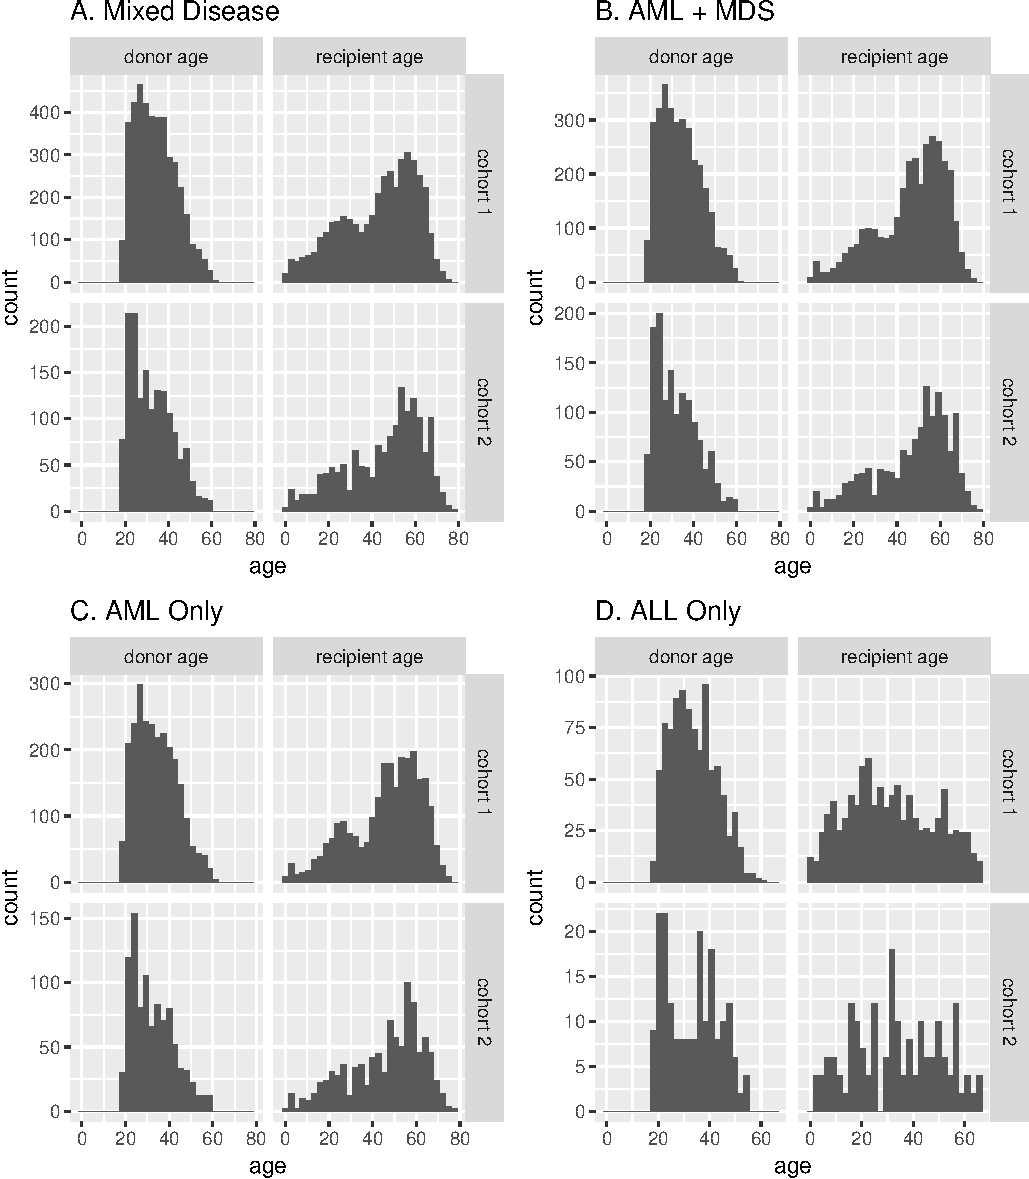
\includegraphics{figures/unnamed-chunk-16-1.pdf}
\caption{\label{fig:age_histograms} Histogram of Donor and Recipient Age
Distributions in (A) Mixed Disease (AML, ALL, and MDS), (B) AML + MDS,
(C) AML only, and (D) ALL only.}
\end{figure}

Additional information that is included from the CIBMTR were
recipient/donor age, recipient/donor sex, recipient BMI, graft source,
Karnofsky performance score, disease status (early, intermediate,
advanced), year of HSCT, and conditioning regimens given prior to
transplant. These meta-data will be incorporated in the statistical
models that will be discussed in the next subsection as well as other
chapters (Figure \ref{fig:age_histograms}).

\subsection{Genotyping and Quality
Control}\label{genotyping-and-quality-control}

All samples were genotyped on a Illumina Human OmniExpress BeadChip
whole-genome genotyping microarray. This chip had 637,655 tagged SNPs
available that were strategically selected from all three phases of the
HapMap project to capture the greatest amount of common SNP variation
(\textgreater{}5\% MAF).

Samples were assigned to plates to ensure the even distribution of
patient characteristics and potential confounding variables using
Optimal Sample Assignment Tool (OSAT), an R/Bioconductor software
package (Yan et al. \protect\hyperlink{ref-OSAT}{2012}). Over 90\% of
DISCOVeRY-BMT patients self-reported as European American, caucasian or
white and thus replication and validation analyses are performed on
these recipient-donor pairs.

An important concept in statistical genetics is \emph{population
stratification} and the necessity to adjust for it when doing
association studies. The association could be due to the underlying
structure of the population and not a disease associated locus. QC is
done to control from those using one of several different available
software. Stringent quality control was performed on both samples and
SNPs within this population. Population outliers were removed using
EIGENSTRAT (A. L. Price et al. \protect\hyperlink{ref-Price_AL}{2006})
(\(n=73\)). Additional sample quality control removed samples with
missing call rate \(\geq 2\%\) (\(n=54\)), sex mismatch (\(n=9\)),
abnormal inbreeding coefficients (n=20), and evidence of cryptic
relatedness (\(n=17\)), yielding 2107 and 777 donor-recipient pairs in
cohorts 1 and 2, respectively. Typed SNPs were removed if the call rate
was \textless{}98\%, there was deviation from Hardy-Weinberg equilibrium
proportions (C. C. Laurie et al.
\protect\hyperlink{ref-laurie2010}{2010}) or discordance between
duplicate samples was \(>2\%\).

Originally, DISCOVeRY-BMT was imputed using IMPUTE2 and 1000 Genomes
Phase 3 data. Again, as the most of the population are of European
ancestry, when HRC was released, DISCOVeRY-BMT was reimputed using HRC
to have higher quality imputation specific to this population due large
number of European samples in HRC.

\section{Statistical Analysis}\label{statistical-analysis}

\subsection{Cox Proportional Hazards
Model}\label{cox-proportional-hazards-model}

Survival models examine the time it takes for events to occur.
Specifically, survival models examine the relationship between survival
(time that passes before some event occurs) and one or more
\emph{covariates} (predictors) that may be associated with that quantity
of time. The Cox proportional hazards regression model (Cox
\protect\hyperlink{ref-cox1972}{1972}) is used for survival analysis and
is our main statistical model of choice. For GWAS, we conduct single SNP
analysis such that each individual SNP is tested under the null
hypothesis of no assocation. SNPs are converted from genotype
probabilities to allele dosage and added to the model as a covariate.

\noindent Assumptions of the Cox model:

\begin{enumerate}
\def\labelenumi{\arabic{enumi}.}
\tightlist
\item
  the regression coefficient (\(\beta\)) is constant over time
  (proportional hazards assumption)\\
\item
  linear combination of covariates\\
\item
  link function is exponential
\end{enumerate}

\subsubsection{Mathematical concepts and
notations}\label{mathematical-concepts-and-notations}

\noindent The Cox model is as follows:

Consider a population of subjects, \(i\), we observe either time to
event or censoring. For the censored individuals, we know that time to
event is greater than censoring time. So the survival function is
\(S(t)\). Let \(T\) represent survival time. \(T\) is a random variable:

\noindent Cumulative distribution function (CDF):\\

\begin{equation} \label{eq1}
P(t) = Pr(T \leq t) 
\end{equation}

\noindent Probability density function (PDF):\\

\begin{equation} \label{eq2}
p(t) = \frac{dP(t)}{dt} 
\end{equation}

\noindent The survival function \(S(t)\) is the complement of the CDF:\\

\begin{equation} \label{eq3}
S(t) = Pr(T \geq t) = 1 - P(t)
\end{equation}

\noindent and the hazard function is \(\lambda(t)\) (or age specific
failure rate). The hazard function, \(\lambda(t)\), is the distribution
of survival times, which assesses the instantaneous risk of dying at
time \(t\), conditional on survival to that time:

\begin{equation} \label{eq4}
\begin{split}
\lambda(t) & = \lim_{\Delta t \to 0}\frac{Pr\big[t \leq T < t + \Delta t) | t \geq T \big]}{\Delta t} \\
    & = \frac{f(t)}{S(t)}
\end{split}
\end{equation}

\noindent Let \(X_i = X_{i1}, ..., X_{ip}\) be realized values of
covariates for subject \(i\). The hazard function for the Cox model has
the form:

\begin{equation} \label{eq5}
\begin{split}
\lambda(t|X_i) & = \lambda_0(t) \cdot \exp(\beta_1 X_{i1} + ... + \beta_p X_{ip}) \\
& = \lambda_0(t) \cdot \exp(X_i^{T} \cdot \beta)
\end{split}
\end{equation}

\noindent This expression gives us the hazard function at time \(t\) for
subject \(i\) with covariate vector \(X_i\). The baseline hazard is a
nuisance parameter and is completely removed. For simplicity, we assume
that there are no tied failure times, although there are methods for
modifying the partial likelihood in the case of ties (Breslow
\protect\hyperlink{ref-breslow1974}{1974}, Efron
(\protect\hyperlink{ref-efron1977}{1977})).

The probability of the event to be observed occurring with subject \(i\)
at time \(Y_i\):

\begin{equation}
\begin{split}
L_i(\beta) & = \frac{\lambda(Y_i|X_i)}{\sum_{j:Y_j \geq Y_i} \lambda(Y_i|X_j)} \\
& = \frac{\lambda_0(Y_i)\exp(X_{i}^{T} \cdot \beta)}{\sum_{j:Y_j \geq Y_i}\lambda_0(Y_i) \exp(X_{j}^{T} \cdot \beta)} \\
& = \frac{\exp(X_{i}^{T} \cdot \beta)}{\sum_{j:Y_j \geq Y_i}\exp(X_{j}^{T} \cdot \beta)}
\end{split}
\end{equation}

\noindent where \(L_{i}(\beta)\) is between 0-1. This is the partial
likelihood function which estimates the beta coefficients without having
to model a time-dependent hazard function.

Assume the subjects are independent of one another (Cox
\protect\hyperlink{ref-cox1972}{1972}), the joint probability of all
realized events takes the partial likelihood form of (occurrence of
event C is \(C_{i} = 1\)):

\begin{equation}
\begin{split}
L_i(\beta) & = \prod_{i:C_{i}=1} L_{i}(\beta)
\end{split}
\end{equation}

We can take the log of this begin estimating the parameters via log
partial likelihood:

\begin{equation}
\begin{split}
\ell(\beta) & = \sum_{i:C_{i}=1}\big(X_{i}^{T}\beta - \log\sum_{j:Y_{j}\geq Y_i}\exp(X_{j}^{T} \cdot \beta) \big)
\end{split}
\end{equation}

We can estimate the model parameters by computing the first order
derivative of the log partial likelihood (score function):

\begin{equation}
\begin{split}
\ell^{\prime}(\beta) & = \sum_{i:C_{i}=1}\Big(X_{i} \frac{\sum_{j:Y_{j}\geq Y_{i}}\exp(X_{j}^{T} \cdot \beta) X_j}{\sum_{j:Y_{j}\geq Y_{i}}\exp(X_{j}^{T} \cdot \beta)} \Big)
\end{split}
\end{equation}

And the Hessian matrix is attainable by computing the second order
deriviative of the log partial likelihood:

\begin{equation}
\begin{split}
\ell^{\prime\prime}(\beta) & = -\sum_{i:C_{i}=1}\Bigg(\frac{\sum_{j:Y_{j}\geq Y_{i}}\exp(X_{j}^{T} \cdot \beta)X_{j}^{\prime}X_{j}}{\sum_{j:Y_{j}\geq Y_{i}}\exp(X_{j}^{T} \cdot \beta)} - \frac{\big[\exp(X_{j}^{T} \cdot \beta) X_{j} \big] \big[\exp(X_{j}^{T} \cdot \beta) X^{\prime}_{j} \big]}{ \big[\exp(X_{j}^{T} \cdot \beta)\big]^{2}}\Bigg)
\end{split}
\end{equation}

The partial likelihood is maximized using the Newton-Raphson method.
Furthermore, standard errors estimates (\(\beta\)) can be approximated
by computing inverse Hessian matrix (an approximation of the
variance-covariance matrix) and taking the diaganol. The standard errors
estimates compute the confidence intervals for the hazard ratio (HR).

\begin{equation}
\begin{split}
\text{HR } [95\%\text{CI}_{\text{LB}}, 95\%\text{CI}_{\text{UB}}] = & \exp(\beta) \big[ \exp(\hat{\beta} - 1.96 \cdot se), \exp(\hat{\beta} + 1.96 \cdot se)\big]
\end{split}
\end{equation}

HRs are reported with every survival analysis result that we discuss
throughout this dissertation. HRs describe the risk over the entire
study period. The interpretation in statistical genetics is that, if
\(\text{HR} > 1\) we report that as risk of the effect allele, if
\(\text{HR} < 1\), we report the HR as protected for a given effect
allele.

\subsubsection{Model Diagnostics}\label{model-diagnostics}

The Cox model can be evaluated in two ways. The proportional hazards
assumption can be tested using Schoenfeld residuals graphically or using
a goodness-of-fit test (Schoenfeld
\protect\hyperlink{ref-schoenfeld1982}{1982}). The model itself can be
validated by simulation. Here will we show both methods. Schoenfeld
residuals are based on the effects of the predictor variables that are
assumed to be independent of time, plotting these residuals versus time
is done to visually assess the effect of the predictor variable and its
relationship with time. A smooth line is fit to the plot of the
residuals (Grambsch and Therneau
\protect\hyperlink{ref-grambsch_ph}{1994}). If the smoothed line has a
slope and intercept of approximately 0, then the proportional hazards
assumption has been met (Grambsch and Therneau
\protect\hyperlink{ref-grambsch_ph}{1994}). The Schoenfeld residuals
were the diagnostic tool used in our lab and were performed and assessed
prior to joining the lab (data not shown).

\subsection{Power Calculations}\label{power-calculations}

We conducted meta-analyses to combine the effects of both cohorts
(discussed in next section below), as such, power calculations were done
considering the sample size of both cohorts combined. Minimum detectable
hazard ratios of recipient and/or donor depend on three variables: 1.)
proportion of individuals experiencing an event, 2.) frequency of a
causal variant, and 3.) the quality of genotyping SNPs that capture the
genetic variation underlying the hazard of an event. Events are measured
at 1 year and at the most updated observation time (most recent
phenotype data available is May 5th, 2017) post-HSCT. The events that
will be measured are death due to transplant (TRM) and specific causes
of death (organ failure, infection, GVHD) attributable to TRM. OS is a
function of TRM and thus we will present minimum detectable hazard
ratios for OS. The proportion of events (Figure 3) ranges from
infrequent events to (i.e.~TRM subtypes) to frequent events (i.e.~OS).
We will assume lower and upper bound causal variant frequency between
5\% and 40\%, respectively. We assumed SNPs selected for genotyping
capture 85\% of the variation across each gene; thus, all power
calculations are corrected by setting our effective total sample size
equal to 0.85 x 3532 = \textasciitilde{}3000. We present the range of
hazard ratios detectable for varying proportions of events and allele
frequencies in a univariate model assuming 80\% power to detect
genome-wide significance at \(5\times{10}^{-8}\). With 3,532
recipient-donor pairs, the minimum detectable hazard ratio under these
assumptions is identical for recipient genotype, donor genotype, and the
mismatch between donor and recipients. Given the minimum proportion of
events experienced in TRM subtypes and overall TRM are between 0.10 and
0.30 with a common allele (MAF=0.40), we have power to detect hazard
ratios between 1.69 and 1.35, respectively. Under these same proportion
of events, with more rare variants (MAF=0.05), we have the power to
detect hazard ratios between 3.3 and 2.0, respectively. For OS models,
assuming the overall rate of death is 0.50, we can detect SNPs in with
hazard ratios between 1.26 (MAF=0.40) and 1.7 (MAF=0.05). Lower bound is
based off each TRM subtype being at least 0.10 (10\%) of all patients.

\begin{figure}
\centering
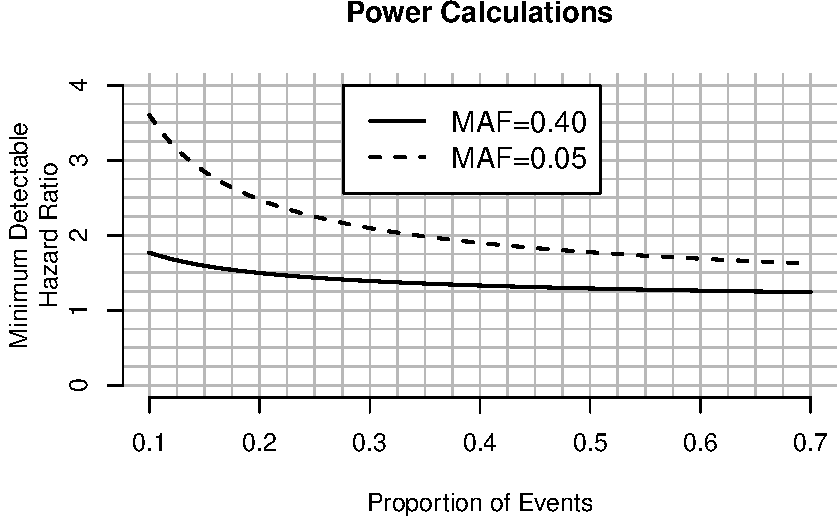
\includegraphics{figures/unnamed-chunk-20-1.pdf}
\caption{Power calculations for DISCOVeRY-BMT. Hazard ratios associated
with survival models.}
\end{figure}

\section{Discussion}\label{discussion}

In this Chapter we laid the foundation for understanding the research
and approaches that were conducted for this dissertation. The first
principles of genetic association studies were discussed, where we
introduced important concepts such as reference panels, population
stratification, genetic imputation, meta-analyses. This was follow by
detailed introduction to DISCOVeRY-BMT cohorts, modeling techniques/
diagnostics and power calcuations that were used for the majority of
this dissertation. DISCOVeRY-BMT is a rich trove of data and can be used
for a multitude of problems, ranging from clinical to statistical
challenges. This remainder of this document will set forth examples of
important aspects of science leveraging these data.

\FloatBarrier

\newpage

\pagestyle{plain} \fancyhead[L]{} \fancyhead[R]{}
\fancyfoot[C]{\thepage}
\chapter{Replication and Validation of Previous HSCT Literature}
\doublespacing

\section{Introduction}\label{introduction-1}

Genetic associations studies usually fall under two main subcategories,
candidate gene association studies (CGAS) or genome wide association
studies (GWAS). CGAS are association studies that investigate specific
genes or regions of interest. Typically these are performed when
researchers believe that the underlying biology is understood and they
want to identify specific markers that contribute to genetic variation
in these `known' regions. For over a decade, researchers in the
hematology and hematological transplant field have conducted CGAS that
investigated the relationship between non-HLA genetics and survival
outcomes after allogeneic transplant. The rationale for conducting the
CGAS was to increase knowledge about clinical management or to serve as
a potential target for novel therapeutics. We exhaustively searched
PubMed for CGAS where the phenotype of interest was survival outcomes
(DRM, TRM, OS, PFS) in patients with ALL, AML, or MDS after HLA-matched
-related-donor (MRD) or -unrelated-donor (MUD) HSCT (Karaesmen et al.
\protect\hyperlink{ref-Karaesmen_2017}{2017}). We identified 70 studies
that reported 45 SNPs in 36 genes as significantly associated with
survival outcomes after transplant. DISCOVeRY-BMT was used to replicate
or validate these published studies (Karaesmen et al.
\protect\hyperlink{ref-Karaesmen_2017}{2017}). The majority of these
studies tested for associations in small datasets, ranging from a few
dozen to a few hundred patients and donors, included heterogeneous
diseases spanning benign to malignant hematological diseases, related
and/or unrelated donors with various degrees of HLA-matching and
patients treated across multiple decades, from the 1980s through early
2000s. In addition to reproducing previous findings, we were interested
in agnostically evaluating whether genes that had been previously
reported upon had an aggregate effect that could be detected and
contributed to survival after transplant.

\section{Methods}\label{methods}

\subsection{Literature Review}\label{literature-review}

An extensive literature search of PubMed was performed using to identify
peer-reviewed scientific studies (published on or before December 30,
2016) that reported non-HLA genetic polymorphisms associated with
survival outcomes after allogeneic BMT, including disease-related
mortality (DRM), progression-free survival (PFS), transplant-related
mortality (TRM) and/or overall survival (OS) (Karaesmen et al.
\protect\hyperlink{ref-Karaesmen_2017}{2017}). The PubMed search terms,
filtering approach are described below:

\singlespaced

\begin{verbatim}
(SNP[Text Word] OR ("polymorphism, genetic"[MeSH Terms] OR
("polymorphism"[All Fields] AND "genetic"[All Fields]) OR
"genetic polymorphism"[All Fields] OR
"polymorphism" [All Fields])) AND
(allo-HSCT[All Fields] OR allo-HCT[All Fields] OR
("unrelated"[All Fields] AND ("donor"[All Fields] OR 
"donors"[All Fields]) AND ("transplant"[All Fields] OR
"transplantation"[All Fields])) OR ("allogeneic"[All Fields] AND
("transplant"[All Fields] OR "transplantation"[All Fields])) OR
("hematopoietic"[All Fields] AND ("transplant"[All Fields] OR
"transplantation"[All Fields]))) AND (("mortality"[Subheading] OR
"mortality"[All Fields] OR "mortality"[MeSH Terms]) OR 
("mortality"[Subheading] OR "mortality"[All Fields] OR
"survival"[All Fields] OR "survival"[MeSH Terms]) OR
(non[All Fields] AND ("recurrence"[MeSH Terms] OR
"recurrence"[All Fields] OR "relapse"[All Fields])) OR
non-relapse[All Fields]) AND English[Language]
\end{verbatim}

\doublespaced

\noindent The Inclusion Criteria comprised of:\\
\noindent Inclusion criteria:\\
1. non-HLA genes\\
2. survival after BMT as phenotype

\noindent Excluded:\\
1. Non-English papers\\
2. Working group studies\\
3. Reviews\\
4. SNPs not in build hg19\\
5. Haplotypes\\
6. Chronic Lymphocytic Leukemia (CML) or multiple myeloma (MM) or
lymphoma only papers\\
7. Autosomal only\\
8. Microsatellites, CNVs, VNTRs, or other variation markers

\subsection{Defintions of Replication and
Validation}\label{defintions-of-replication-and-validation}

In principle, results from CGAS or GWAS should be reproduced in an
independent study to confirm findings (Colhoun, McKeigue, and Smith
\protect\hyperlink{ref-colhoun2003}{2003}; Martin et al.
\protect\hyperlink{ref-martin_2016}{2016}). Two distinctive terms have
gained popularity amongst researchers to describe reproducibility --
specifying if there are differences between the original population that
was studied and the confirmation study: replication and validation (Igl,
Konig, and Ziegler \protect\hyperlink{ref-Igl_2009}{2009}). Replication
is deemed to be when the inclusion criteria are near or completely
identical (i.e.~same ancestral population), so that any differences
between the samples in the study can attributed to random variation
(Igl, Konig, and Ziegler \protect\hyperlink{ref-Igl_2009}{2009}).
Validation reproducibility is when the original and confirmation study
have similar but slightly different inclusion criteria (i.e.~different
ancestral populations. In the validation case, the underlying
differences between the original and confirmation study can be
attributed to systematic variation (Igl, Konig, and Ziegler
\protect\hyperlink{ref-Igl_2009}{2009}).

Thus, replication analyses were conducted when the original study
included HLA MUD-HSCT in patients of European ancestry. Validation
analyses were performed on studies of leukemia patients of non-European
ancestry, patient populations who received MRD-HSCT, or patient
populations that were mixed between those who received a MRD-HSCT and
MUD-HSCT (Karaesmen et al.
\protect\hyperlink{ref-Karaesmen_2017}{2017}). For studies of outcomes
involving multiple hematologic malignancies, the entire DISCOVeRY-BMT
study population was analyzed. If the original study population was
specified as AML, ALL and/or MDS, the same disease inclusion criteria
were applied so that the replication/validation study population aligned
with that of the original study population.

\begin{figure}
\centering
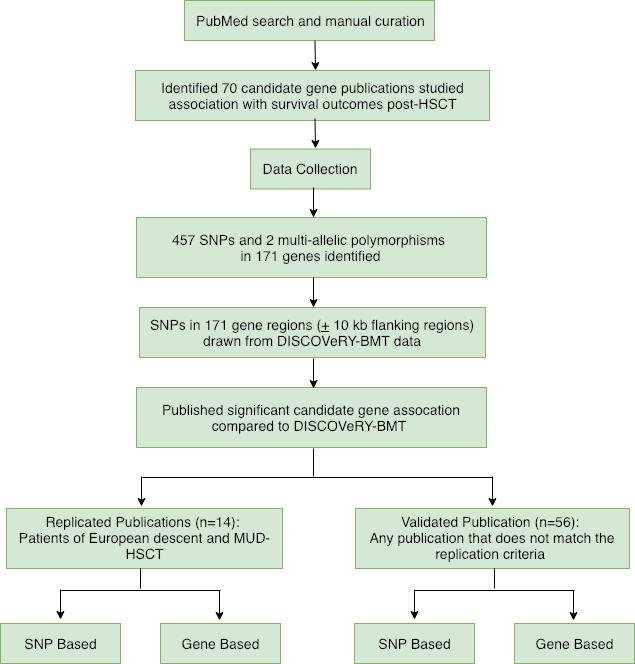
\includegraphics{~/Desktop/figures/chapter2/repval_fig1.png}
\caption{Pipeline performed for reproducing previous candidate gene
association study literature}
\end{figure}

\subsection{Genotyping data}\label{genotyping-data}

All samples were genotyped using the Illumina Human OmniExpress BeadChip
and the Illumina HumanExome BeadChip (University of Southern California
Genomics Facility). In total, 637,655 and 632,823 SNPs from the
OmniExpress BeadChip were available for imputation in cohorts 1 and 2,
respectively, using 1000 Genomes Project phase 3. The missing genotypes
were imputed using IMPUTE2 software (B. N. Howie, Donnelly, and Marchini
\protect\hyperlink{ref-Howie_2009}{2009}). QCTOOL was used to remove
imputed genotypes with an info score \textgreater{} 0.7, certainty
\textgreater{} 0.7, and a minor allele frequency \(\geq\) 0.005. To test
the joint effect of recipient and donor genetic variation, the
recipient-donor (R-D) \emph{mismatch} genome computed by taking the
absolute value of the difference of minor alleles between recipient and
donor at each SNP. For example, at a given SNP where the recipient is
homozygous minor (2 minor alleles) and the donor is heterozygous (1
minor allele), the mismatch allele dosage would be \(|2-1|=1\).
Rs2066847 (SNP13) in \emph{NOD2/CARD15} was the only variant analyzed
from the Illumina HumanExome, as it was not typed on the OmniExpress
chip or available following imputation.

\subsection{Genetic Models}\label{genetic-models}

Prior to genetic analyses, clinical covariates for inclusion in
genome-wide survival models were selected using bidirectional stepwise
regression (Venables and Ripley
\protect\hyperlink{ref-Venables_2002}{2002}) on Cox proportional hazard
models (Cox \protect\hyperlink{ref-cox1972}{1972}) of OS, PFS, TRM and
DRM using R statistical software (R Core Team
\protect\hyperlink{ref-r_core}{2018}). Cox proportional hazard models of
OS, TRM and DRM evaluated SNPs associated with time to death with all
survivors censored at 1 year post-HSCT (Therneau and Grambsch
\protect\hyperlink{ref-therneau2013}{2013}). PFS was defined as the time
to disease progression or death. The covariates that were included in
the model were (see
\href{https://github.com/aarizvi/dissertation/tree/master/code/chapter2}{Appendix
GitHub} for R code):\\
1. OS -- recipient age, disease status (early or advanced), graft source
(bone marrow or peripheral blood)\\
2. DRM -- recipient age, disease status (early or advanced)\\
3. TRM -- recipient age, body mass index (BMI) (underweight, normal,
overweight, obese), graft source (bone marrow or peripheral blood)\\
4. PFS -- recipient age, disease status (early or advanced)

Depending on the disease group, disease types were adjusted for by
creating an indicator variables. E.g. For analyses without ALL (AML and
MDS), the indicator variable AML dummy and MDS dummy were added to the
model. Competing risk models (Fine and Gray
\protect\hyperlink{ref-fine1999}{1999}) were used for TRM and DRM
(because a patient can only die once). Dosage data accounting for the
probability of each genotype were used in all analyses of imputed data.
Effect size estimates and standard errors from DISCOVeRY-BMT Cohorts 1
and 2 were compared and combined using a fixed-effects inverse variance
meta-analyses in METAL (Willer, Li, and Abecasis
\protect\hyperlink{ref-metal}{2010}). For each SNP, heterogeneity of
effect size estimates between cohorts 1 and 2 was assessed using
p-values from significance tests of heterogeneity (\(P_{het}\)) and
\(I^{2}\). Variants with \(P_{het}\) \textless{} 0.05 and \(I^{2}>50\)
were meta-analyzed with a random effects models using meta (Schwarzer
\protect\hyperlink{ref-Schwarzer_2007}{2007}) in R.

\subsubsection{Multi-allelic models}\label{multi-allelic-models}

\emph{NOD2/CARD15} was the most common gene studied in the HSCT
literature. The associations were based on a 3-variant R-D pair model
(rs2066844 {[}SNP8{]}, rs20666845 {[}SNP12{]}, rs2066847 {[}SNP13{]})
and single SNP associations with SNP13 (Ernst Holler et al.
\protect\hyperlink{ref-holler_2004}{2004}). The null type was when the
R-D pair are homoyzgous common allele for all 3 SNPs and the effect
allele combination was considered the presence of \(/geq\) 1 minor
allele in any of the 3 SNPs within the R-D pair. \emph{CCR5} haplotype
was studied in one replication study (McDermott et al.
\protect\hyperlink{ref-mcdermott2010}{2010}). The risk H1/H1 haplotype
was defined as presence of homozgous genotype for the major allele at
rs1799987 (AA), rs1800023 (AA), rs333
(ACAGTCAGTATCAATTCTGGAAGAATTTCCAG); individuals not homozygous common
were considered null. rs333, a 32-basepair deletion, was not typed or
imputed in the DISCOVeRY-BMT cohort, however we selected a proxy SNP
(rs1133418) in strong linkage disequilibrium (\(r^2=0.97\)) with rs333.
The presence of the G allele in the proxy SNP corresponds to
ACAGTCAGTATCAATTCTGGAAGAATTTCCAG in rs333. McDermott and colleagues
(2010) defined 3 risk subgroups:\\
1. R-D Group 1 -- R-D pairs lacked \emph{CCR5} H1/H1 haplotype\\
2. R-D Group 2 -- donors only had \emph{CCR5} H1/H1 haplotype\\
3. R-D Group 3 -- recipients only had \emph{CCR5} H1/H1 haplotype

\noindent The imputed data for \emph{CCR5} was in the IMPUTE2 output
data chunk for chromosome 3
(\texttt{BMT093013\_forImpute.chr3-45000000-50000000.impute2}). QCTOOL
was used to extract the data out from the IMPUTE2 and output it into the
a VCF file. The location for these files was stored on the University at
Buffalo Computational Center Resource (UB CCR) supercomputer. See
\href{https://github.com/aarizvi/dissertation/tree/master/code/chapter2}{Appendix
GitHub} for full code on analysis.

\singlespacing

\begin{Shaded}
\begin{Highlighting}[]
\ExtensionTok{qctool} \DataTypeTok{\textbackslash{} }
    \ExtensionTok{-g}\NormalTok{ ./BMT093013_forImpute.chr3-45000000-50000000.impute2 \textbackslash{}}
\NormalTok{    -s ./BMT093013_forImpute.chr16-50000000-55000000.impute2_samples \textbackslash{}}
\NormalTok{    -og ./ccr5_rep_dosages_threshold.vcf \textbackslash{}}
\NormalTok{    -incl-rsids ccr5_snps.txt }
\end{Highlighting}
\end{Shaded}

\doublespacing
\noindent The data wrangling to prepare the data for these models was
done in R. The Cox survival models were written and automated with
custom R code that leveraged the survival package (Therneau and Grambsch
\protect\hyperlink{ref-therneau2013}{2013}) (see
\href{https://github.com/aarizvi/dissertation/tree/master/code/chapter2}{Appendix
GitHub} for code used for the full analysis).

\subsection{Gene-based assocation
testing}\label{gene-based-assocation-testing}

VErsatile Gene-based Association Study 2 (VEGAS2) software was used for
gene-based association testing (Mishra and Macgregor
\protect\hyperlink{ref-Mishra_2015}{2015}). VEGAS2 uses \(10^{6}\) Monte
Carlo simulations to test the global significance of an association for
sets of SNPs in defined genomic regions. VEGAS2 reports a gene-based
P-value for each gene determined using individual SNP association
P-values. Directional effects are not incorporated into analyses; thus,
all SNPs can be aggregated without dampening an association signal. For
the gene-based replication or validation analyses, the P-values from
typed and imputed SNPs in DISCOVeRY-BMT (\(\pm\) a 10kb flanking region)
meta-analyses of OS, PFS, TRM and DRM were used as input into the VEGAS2
software. Gene-based P-values were calculated for donor, recipient, and
R-D mismatch analyses of the full cohort (ALL, AML and MDS patients) or
homogeneous disease subgroups (ALL or AML or MDS patients) corresponding
to the analyses performed in the original studies (Karaesmen et al.
\protect\hyperlink{ref-Karaesmen_2017}{2017}).

To run VEGAS2, a flat text file is needed that has two unlabeled columns
(rsid and GWAS P-value {[}\(P_{meta}\){]}).

\noindent For example:

\singlespaced

\begin{Shaded}
\begin{Highlighting}[]
\CommentTok{#snps.txt}
\ExtensionTok{rs6696752}\NormalTok{   0.827182998293298}
\ExtensionTok{rs72638700}\NormalTok{  0.874653327370856}
\end{Highlighting}
\end{Shaded}

\doublespaced

\noindent And then a simple command prompting VEGAS2 is run on the
command line:

\singlespaced

\begin{Shaded}
\begin{Highlighting}[]
\ExtensionTok{vegas2}\NormalTok{ \textbackslash{}}
\NormalTok{    snps.txt \textbackslash{}}
\NormalTok{    -pop 1000GEURO \textbackslash{}}
\NormalTok{    -subpop EURO \textbackslash{}}
\NormalTok{    -genesize 10kbloc \textbackslash{}}
\NormalTok{    -top 100 \textbackslash{}}
\NormalTok{    -sex BothMnF \textbackslash{}}
\NormalTok{    -max 1000000 \textbackslash{}}
\NormalTok{    -out ./results/output_V2out }
\end{Highlighting}
\end{Shaded}

\doublespaced
\noindent VEGAS2 analyses were using SNPs from all of the identified
genes and p-values from DISCOVeRY-BMT (for all outcomes and 3 genomes)
on UB CCR (see
\href{https://github.com/aarizvi/dissertation/tree/master/code/chapter2}{Appendix
GitHub}).

\subsection{Functional Annotation}\label{functional-annotation}

To gain a deeper understanding of genetic associations, often
bioinformatics approaches leverage the plethora of curated, publically
available datasets and databases (Gallagher and Chen-Plotkin
\protect\hyperlink{ref-gallagher_2018}{2018}). The databases used in
this study were RegulomeDB (Boyle et al.
\protect\hyperlink{ref-Boyle_2012}{2012}), Blood expression quantitative
trait loci (eQTL) Browser (Westra et al.
\protect\hyperlink{ref-westra_2013}{2013}), and Variant Effect Predictor
(VEP) (McLaren et al. \protect\hyperlink{ref-vep_2010}{2010}), which
were used to annotate the SNPs in the candidate genes. For RegulomeDB
and Blood eQTL Browser, the full database consisting of raw data scores,
P-values, and annotations were downloaded. VEP annotation was done
directly on VEP's website.

RegulomeDB stores variant annotation with known and predicted regulatory
DNA elements in humans. The elements include DNase hypersensitivity,
transcription factor (TF) binding sites, and promoter regions that have
been characterized to alter transcription (Boyle et al.
\protect\hyperlink{ref-Boyle_2012}{2012}). RegulomeDB database compiled
these annotations using the publically available data sets from the
Encyclopedia of DNA elements (ENCODE) project and the Roadmap Epigenome
Consortium and Gene Expression Omnibus (GEO). RegulomeDB scores are the
following: 1a-1f likely to affect TF binding and linked to altering
expression of target genes; 2a-2c likely to affect TF binding; 3a-3b
less likely to affect TF binding, and \textgreater{} 3 has minimal
binding evidence. RegulomeDB DB scores are assigned (only one per SNP)
based on the level of effect and evidence of functional modification
that is attributable to the SNP across multiple cell lines from
differing tissues. The scores are supported by experimental evidence,
with scores from 1 to 7, with 1 having the greatest functional effect,
and scores of 7 show no evidence of having modifying effects.

Blood eQTL database was built from a study (\(N=5000\)) that
investigated the correlation between genetic expression and genetic
polymorphisms and replicated the results in an independent study
(\(N \approx 3000\)), Westra et al.
(\protect\hyperlink{ref-westra_2013}{2013}){]}. We only considered
\emph{cis}-eQTLs, defined as \textless{} 250KB distance between the SNP
chromosomal position and the probe midpoint for gene expression.
Furthermore, VEP was used to determine the hypothetical (predicted)
functional importance of missense and nonsense variants based on SIFT,
Mutation Taster and PolyPhen-2 software.

\section{Results}\label{results}

\subsection{Candidate Gene Studies of Survival
Outcomes}\label{candidate-gene-studies-of-survival-outcomes}

\begin{figure}
    \centering
    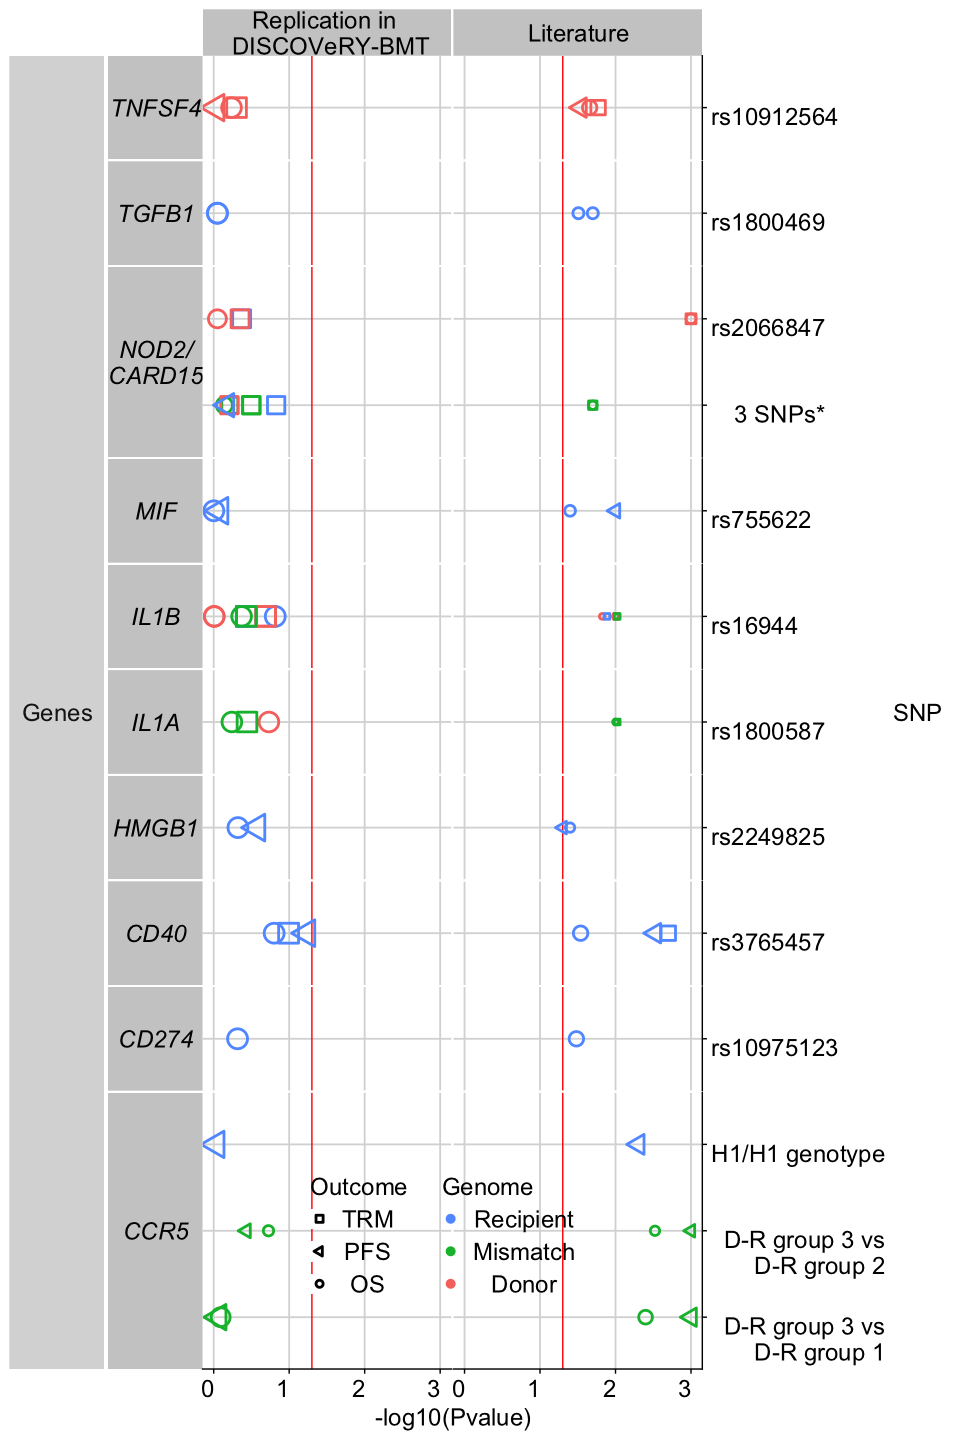
\includegraphics[width=\linewidth, height=6in]{~/Desktop/figures/chapter2/Replication_Fig.png}
    \caption[Replication attempts of previously reported significant candidate gene-association studies in DISCOVeRY-BMT.]{Replication attempts of previously reported significant candidate gene-association studies in DISCOVeRY-BMT. Survival association P values as reported in previous literature (Right panel) and replication attempts of these associations in DISCOVeRY-BMT cohort (Left panel) are shown as data points. Vertical panels indicate the genes that these polymorphisms and haplotypes are located in or close to as reported by the previous studies. Shapes represent associations with survival outcomes OS, PFS, or TRM; colors correspond to donor, recipient, or donor-recipient mismatch polymorphisms. The size of the point represents the sample size of the study, with larger points reflecting a bigger sample size. Shown on y-axis are the 9 polymorphisms from the literature reporting associations at $P<0.05$ with OS, PFS, or TRM by 1 or more previously published studies; the x-axis is the $\log_{10}(\text{P-value})$. The red vertical lines in (left panel) and (right panel) indicate $P<0.05$. Details on the haplotypes are described in “Results” under “Replication.”}
    \label{fig:rep_fig}
\end{figure}

\afterpage{
\begin{landscape}

\rowcolors{2}{gray!6}{white}
\begin{table}[t]

\caption{\label{tab:unnamed-chunk-24}\label{tab:repval_table} Count of reports with SNPs that were studied at least twice (in addition to CCR5 studies) that were attempted for replication or validation in DISCOVeRY-BMT.}
\centering
\fontsize{7}{9}\selectfont
\begin{tabular}{>{\raggedright\arraybackslash}p{8.15em}|>{\raggedright\arraybackslash}p{6em}|>{\raggedleft\arraybackslash}p{9.2em}|>{\raggedleft\arraybackslash}p{9.2em}|>{\raggedleft\arraybackslash}p{9.4em}|>{\raggedleft\arraybackslash}p{9.4em}|>{\raggedleft\arraybackslash}p{9.1em}|>{\raggedleft\arraybackslash}p{9.1em}}
\hiderowcolors
\hline
SNP & Gene & Reports of SNPs with any HSCT outcome & Significant SNPs with any HSCT outcome & Reports of SNPs European ancestry MUD-HSCT populations & Significant SNPs in European ancestry MUD-HSCT populations & Reports of SNPs tested non-European ancestry and/or MRD-HSCT populations & Significant SNPs in non-European ancestry and/or MRD-HSCT populations\\
\hline
\showrowcolors
rs1045642 & ABCB1 & 3 & 1 & 0 & 0 & 3 & 1\\
\hline
rs2032582 & ABCB1 & 2 & 1 & 0 & 0 & 2 & 1\\
\hline
\textasciicircum{} R-D Group 3 vs R-D Group 1 & CCR5 & 1 & 1 & 1 & 1 & 0 & 0\\
\hline
\textasciicircum{} R-D Group 3 vs R-D Group 2 & CCR5 & 1 & 1 & 1 & 1 & 0 & 0\\
\hline
H1/H1 genotype & CCR5 & 1 & 1 & 1 & 1 & 0 & 0\\
\hline
rs2569190 & CD14 & 2 & 1 & 0 & 0 & 2 & 1\\
\hline
rs231775 & CTLA4 & 9 & 4 & 1 & 0 & 8 & 4\\
\hline
rs3087243 & CTLA4 & 9 & 2 & 1 & 0 & 8 & 2\\
\hline
rs5742909 & CTLA4 & 6 & 1 & 0 & 0 & 6 & 1\\
\hline
rs4553808 & CTLA4 & 5 & 1 & 1 & 0 & 4 & 1\\
\hline
rs4244285 & CYP2C19 & 2 & 1 & 0 & 0 & 2 & 1\\
\hline
rs8192917 & GZMB & 2 & 1 & 0 & 0 & 2 & 1\\
\hline
rs1800587 & IL1A & 3 & 1 & 0 & 0 & 3 & 1\\
\hline
rs16944 & IL1B & 4 & 1 & 0 & 0 & 4 & 1\\
\hline
rs1800587 & IL1B & 3 & 1 & 0 & 0 & 3 & 1\\
\hline
rs11209026 & IL23R & 3 & 2 & 0 & 0 & 3 & 2\\
\hline
rs1800795 & IL6 & 5 & 3 & 0 & 0 & 5 & 3\\
\hline
rs1800797 & IL6 & 3 & 1 & 0 & 0 & 3 & 1\\
\hline
rs1801133 & MTHFR & 4 & 3 & 0 & 0 & 4 & 3\\
\hline
rs1801131 & MTHFR & 3 & 1 & 0 & 0 & 3 & 1\\
\hline
3 SNPs* & NOD2/ CARD15 & 9 & 4 & 2 & 1 & 7 & 3\\
\hline
rs2066847 & NOD2/ CARD15 & 4 & 2 & 1 & 1 & 3 & 1\\
\hline
rs2066842 & NOD2/ CARD15 & 3 & 1 & 0 & 0 & 3 & 1\\
\hline
rs9658254 & NOS1 & 2 & 1 & 0 & 0 & 2 & 1\\
\hline
rs1800469 & TGFB1 & 3 & 1 & 1 & 1 & 2 & 0\\
\hline
rs4986790 & TLR4 & 2 & 1 & 0 & 0 & 1 & 1\\
\hline
rs731236 & VDR & 5 & 2 & 0 & 0 & 5 & 2\\
\hline
rs7975232 & VDR & 5 & 2 & 0 & 0 & 5 & 2\\
\hline
\multicolumn{8}{l}{\textbackslash{}\textbackslash{}\textasciicircum{}\{\textasciicircum{}\} CCR5 H1/H1 genotypes and risk groups defined using multiallelic models described in the original publication (McDermott et al 2010) and in the main text.}\\
\multicolumn{8}{l}{3 SNPs* -- The NOD2/CARD15 3 SNP multiallelic model. Described in the text.}\\
\end{tabular}
\end{table}
\rowcolors{2}{white}{white}

\end{landscape}
}

The literature search identified 70 publications that studied a total
458 SNPs and 2 multi-allelic polymorphisms in 171 genes (Figure 2.1).
Studies included patients who received a transplant from an MUD-HSCT (19
articles), a MRD-HSCT (23 articles), or both (28 articles) (Table
\ref{tab:repval_table}). Study populations included patients and donors
of European ancestry (53 articles), Asian ancestry (15 articles), or
mixed genomic ancestry (2 articles) (Table \ref{tab:repval_table}).

\normalsize

\doublespacing

A total of 14 articles assessed genetic variation in HLA MUD-HSCT
patients of European ancestry, but only 7 of these articles reported
significant associations (\(P < 0.05\) or an author specified
significance threshold) and thus comprise our replication study (Table
\ref{tab:repval_table}, Figure \ref{fig:rep_fig}). A total of 56
articles tested associations in either a combination of MRD and
MUD-HSCT, only MRD and/or in non-European populations; 39 of these 56
articles reported at least one significant SNP association with survival
outcome and we attempted to validate the significant findings from these
39 articles (Table \ref{tab:repval_table}, \ref{fig:val_fig}) (Karaesmen
et al. \protect\hyperlink{ref-Karaesmen_2017}{2017}).

\subsection{Replication}\label{replication}

To reproduce previous reported results, DISCOVeRY-BMT was used to
replicate findings that comprised of acute leukemia or MDS patients with
European ancestry, treated with MUD-HSCT (Karaesmen et al.
\protect\hyperlink{ref-Karaesmen_2017}{2017}). Seven articles were
included in the replication analyses. Multi-allelic models, \emph{CCR5}
and \emph{NOD2/CARD15}, were tested in 2 articles; single SNP
associations in \emph{CD274}, \emph{CD40}, \emph{HMGB1}, \emph{IL1A},
\emph{IL1B}, \emph{NOD2/CARD15}, \emph{TGFB1}, and \emph{TNFSF4} were
tested in 5 articles (Table \ref{tab:repval_table}, Figure
\ref{fig:rep_fig}) (Karaesmen et al.
\protect\hyperlink{ref-Karaesmen_2017}{2017}).

As previously discussed, candidate genes and candidate SNPs are selected
due to \emph{a priori} biological knowledge of the phenotype. The
general thought in HSCT is that patients are either dying from their
disease or from the transplant. And transplant related causes are mostly
infection, organ failure, or GVHD. Relevant biological pathways that are
included in these phenotypes are likely to involve immunological and
inflammatory pathways. Indeed, the most frequently studied gene was
\emph{NOD2/CARD15}, which is a susceptibility gene for inflammatory
bowel disease and may be involved in Crohn's disease (E Holler et al.
\protect\hyperlink{ref-holler_2008}{2008}) (Table
\ref{tab:repval_table}). The two \emph{NOD2/CARD15} associations were
based on a three-variant R-D pair model {[}rs2066844 (SNP8), rs2066845
(SNP12) and rs2066847 (SNP13){]} and single SNP associations with SNP13
(E Holler et al. \protect\hyperlink{ref-holler_2008}{2008}). The null
genotype is when the R-D pair are homozygous common allele for all 3
SNPs and the effect allele combination is the presence of 1 or more
minor alleles at any of the 3 SNPs within the R-D pair. The
\emph{NOD2/CARD15} multi-SNP model was significantly associated with OS
(RR: 1.6, 95\% CI 1.1-2.4, \(P=0.02\)) and TRM (RR: 1.6, 95\% CI
1.1-2.4, \(P=0.02\)) in a study of 196 patients who received a MUD-HSCT
for AML or ALL. However, no associations were found for OS (HR: 1.03,
95\% CI 0.9-1.2, \(P=0.72\)) or TRM (HR: 1.1, 95\% CI 0.8-1.4,
\(P=0.6\)) in DISCOVeRY-BMT, which is a larger study (\(N=1597\)) with
AML and ALL patients treated with MUD-HSCT (Figure \ref{fig:rep_fig}).
Furthermore, a study of 342 AML or ALL patients after MUD-HSCT (E Holler
et al. (\protect\hyperlink{ref-holler_2008}{2008})) reported donor
genotype rs2066847 (SNP13) significantly increased risk of TRM and OS
approximately 3-fold (\(P=0.001\)) and 2.5 (\(P=0.001\)), respectively.
When this SNP was tested in DISCOVeRY-BMT donors, no associations were
found with either TRM (HR: 1.17, 95\% CI 0.78-1.74, \(P=0.45\)) or OS
(HR: 0.98, 95\% CI 0.73-1.31, \(P=0.89\), in ALL or AML patients)
(Figure \ref{fig:rep_fig}).

One of the largest CGAS (\(N=1370\)) reported significant associations
for \emph{CCR5} H1/H1 genotype (\(N=163\)) in recipients (McDermott et
al. \protect\hyperlink{ref-mcdermott2010}{2010}). McDermott and
colleagues also defined genotype risk subgroups and OS (Figure
\ref{fig:rep_fig}; able \ref{tab:repval_table}). These associations were
tested in DISCOVeRY-BMT and neither \emph{CCR5} H1/H1 genotype (N=294)
nor the genotype risk groups defined by H1/H1 status were significantly
associated with PFS or OS (Figure \ref{fig:rep_fig}, Table
\ref{tab:repval_table}). The genotype risk groups (Group 3 vs Group 1
and Group 3 vs Group 2) were substantially smaller than the full cohort.
We tested these in DISCOVeRY-BMT and found no associations. Considering
the fact that DISCOVeRY-BMT cohorts were approximately twice as large as
those in the original study and adequately powered to detect these
associations (Figure 1.11), these risk group associations were not real
(Karaesmen et al. \protect\hyperlink{ref-Karaesmen_2017}{2017}). In
DISCOVeRY-BMT these subgroups were approximately twice as large as those
in the original study and adequately powered to detect these
associations.

DISCOVeRY-BMT was unable to replicate another large CGAS of 1170
patients (Jindra et al. \protect\hyperlink{ref-jindra_2016}{2016}),
which reported an association between rs10912564 (\emph{TNFSF4}) and TRM
(\(P=0.017\)), OS (\(P=0.022\)), and PFS (HR: 0.8, 95\% CI
{[}0.9-1.2{]}, \(P=0.03\)) (Figure \ref{fig:rep_fig}). Similarly
DISCOVeRY-BMT could not replicate rs2249825 in \emph{HMGB1} (Kornblit et
al. \protect\hyperlink{ref-kornblit_2010}{2010}, N=276), rs1800469 in
\emph{TGFB1} (Arrieta-Bolaños et al.
\protect\hyperlink{ref-bolanos_2016}{2016}, N=493), rs755622 in
\emph{MIF} (Chang et al. \protect\hyperlink{ref-chang_2009}{2009},
N=454), nor SNPs in \emph{IL1A} and \emph{IL1B} (Figure
\ref{fig:rep_fig}).

\subsection{Validation}\label{validation}

\begin{figure}
    \centering
    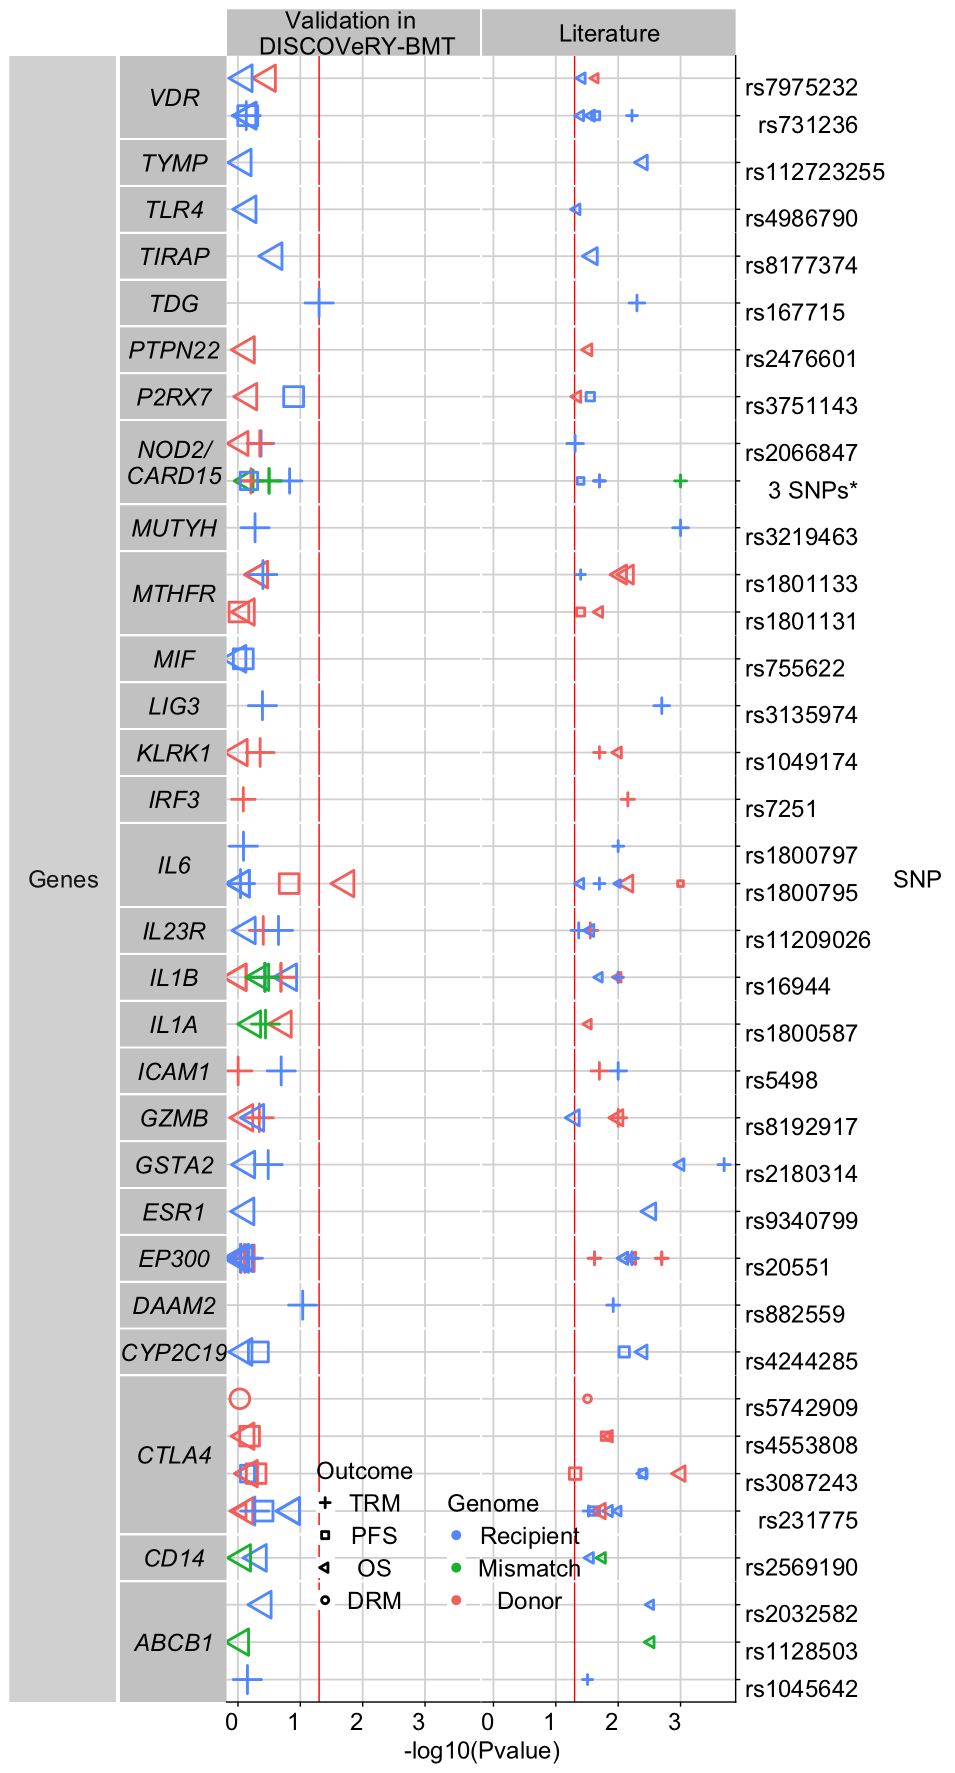
\includegraphics[width=\linewidth, height=6in]{~/Desktop/figures/chapter2/Validation_Fig.png}
    \caption[Validation attempts of previously reported significant candidate gene-association studies.]{Validation attempts of previously reported significant candidate gene-association studies. Survival association P-values as reported in previous literature (Right panel) and validation attempts of these associations in DISCOVeRY-BMT cohort (Left panel) are shown as data points. Vertical panels indicate the genes that these 17 polymorphisms are located in or closest to as reported by the previous studies. Shapes represent associations with survival outcomes DRM, OS, PFS, and TRM; colors correspond to donor, recipient, or donor-recipient mismatch polymorphisms. The size of the point represents the sample size of the study, with larger points reflecting a bigger sample size. Shown on y-axis are the 17 polymorphisms from the literature reporting associations at $P < 0.05$ with OS, PFS, or TRM by 1 or more previously published studies; the x-axis is the $\log_{10}(\text{P-value})$. The red vertical lines in (left panel) and (right panel) indicate $P < 0.05$. Details on the haplotypes are described in “Results” under “Validation."}
    \label{fig:val_fig}
\end{figure}

Validation attempts were conducted on 36 genetic polymorphisms in 26
genes from 39 previously published CGAS (Table \ref{tab:repval_table}).
The genes that were included: \emph{ABCB1}, \emph{CD14}, \emph{CTLA4},
\emph{CYP2C19}, \emph{DAAM2}, \emph{EP300}, \emph{ESR1}, \emph{GSTA2},
\emph{GZMB}, \emph{ICAM1}, \emph{IL23R}, \emph{IL6}, \emph{IRF3},
\emph{KLRK1}, \emph{LIG3}, \emph{MTHFR}, \emph{MUTYH},
\emph{NOD2/CARD15}, \emph{NOS1}, \emph{P2RX7}, \emph{TDG}, \emph{TIRAP},
\emph{TLR4}, \emph{TYMP}, and \emph{VDR} (Figure \ref{fig:val_fig})
(Karaesmen et al. \protect\hyperlink{ref-Karaesmen_2017}{2017}). Each of
these studies reported at least one significant genetic associations
with survival in patients who received a HLA MRD-HSCT (19 articles) or
had a study population including MRD- and MUD-HSCT patients, without
stratification of results (17 articles). Validation attempts for
survival associations reported in non-European leukemia patients who
received an MUD-HSCT (3 articles) (Table \ref{tab:repval_table}). The
variants that had been reported to be associated to survival outcomes
after transplant and our attempts to validate the results in
DISCOVeRY-BMT are shown in Figure \ref{fig:val_fig}.

Only one of our validation attempts were successfully reproduced --
where donor genotype rs1800795 (\emph{IL-6}) was associated with OS (HR:
1.11, 95\% CI 1.0-1.2, \(P=0.02\)) (Figure \ref{fig:val_fig}, note: this
did not reach genome-wide significance at the \(P < 5\times{10}^{-8}\)
threshold). The rs1800795 association to OS (HR: 1.29, 95\% CI
1.07-1.55, \(P=0.007\)) was reported in a single study in patients with
acute leukemia, CML, or lymphoma (N=743) treated with MRD- or MUD-HSCT
(Balavarca et al. \protect\hyperlink{ref-balavarca_2015}{2015}).

Similar to our replication set, \emph{NOD2/CARD15} was the most
frequently studied gene and reported the most of all CGAS in our
validation set (Table \ref{tab:repval_table}). Three studies reported
associations between the presence of \emph{NOD2/CARD15} multi-SNP
polymorphism and either TRM (Ernst Holler et al.
\protect\hyperlink{ref-holler_2004}{2004}) or PFS. None of these studies
were validated in DISCOVeRY-BMT cohorts (Figure \ref{fig:val_fig}).
Likewise, DISCOVeRY-BMT was unable to validate single SNP analyses in
\emph{NOD2/CARD15} for rs2066842 in MRD- or MUD-HSCT donors with PFS or
for TRM at rs2066847 (SNP13) in recipients of MRD- or MUD-HSCT (Figure
\ref{fig:val_fig}).

\begin{figure}
    \centering
    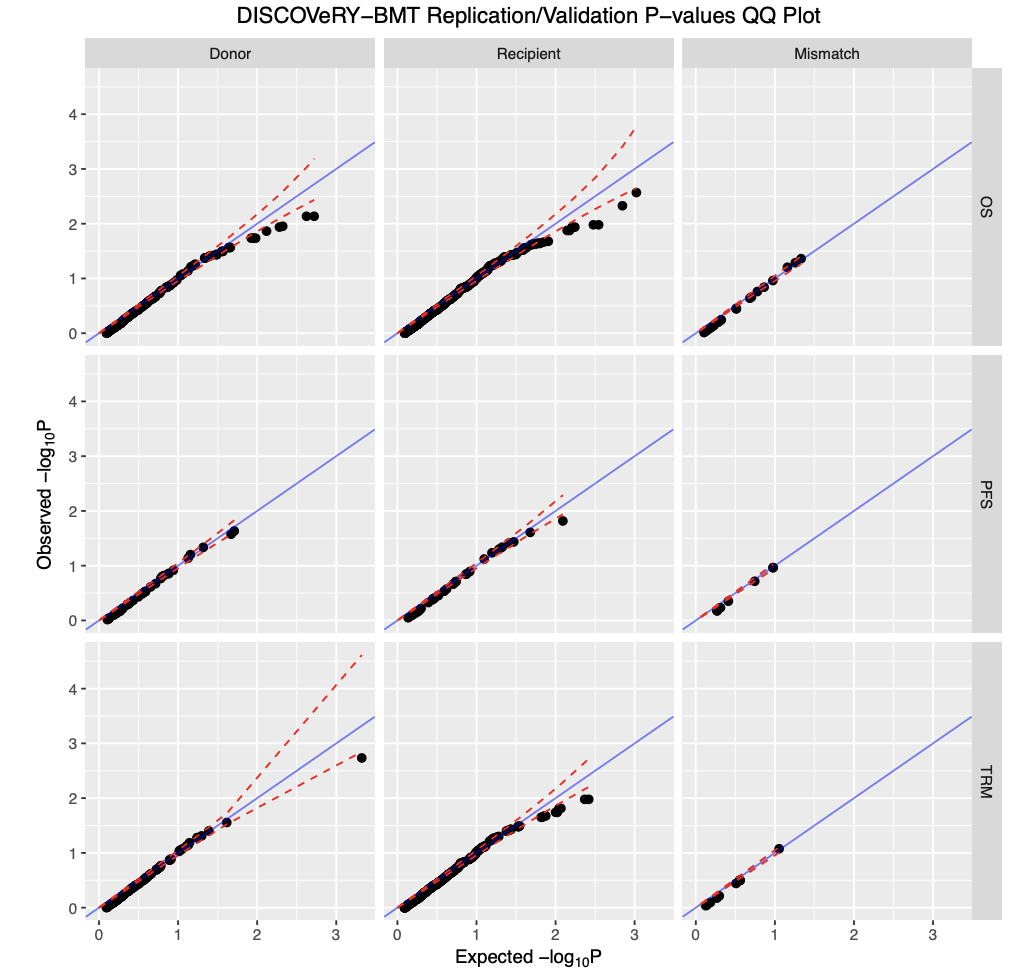
\includegraphics[width=\linewidth, height=3.5in]{~/Desktop/figures/chapter2/ch2_cg_qqplot.png}
    \caption[Quantile-quantile (QQ) plot of SNP p-values in DISCOVeRY-BMT for all previously studied SNPs.]{Quantile-quantile (QQ) plot of SNP p-values in DISCOVeRY-BMT for all previously studied SNPs. From left to right, vertical panels represent the donor, recipient, and mismatch genome, horizontal panel represents the survival outcome that was tested, from top to bottom overall survival (OS), progression free survival (PFS) and transplant related mortality (TRM). Dashed red lines indicate 95\% confidence intervals}
    \label{fig:qq_genes}
\end{figure}

\emph{CTLA4} is a member of the immunoglobulin superfamily that is
expressed by activated T-cells and transmits inhibitory signal to
T=cells. Due to these known functions and perceived implications in
transplant biology, associations with multiple SNPs in \emph{CTLA4} have
been tested in numerous transplant populations (Table
\ref{tab:repval_table}; Pérez-García et al.
(\protect\hyperlink{ref-perez_garcia_2007}{2007})). In previous CGAS,
four \emph{CTLA4} SNPs (rs3087243, rs231775, rs4553808, rs5742909) were
significantly associated with survival after MRD- or MUD-HSCT in
patients with acute leukemia, CML, lymphomas, MDS, and other
hematological disorders (Table \ref{tab:repval_table}). Attempts to
validate CTLA4 SNPs with DRM, PFS, OS, and TRM were unsuccessful in the
DISCOVeRY-BMT cohorts (Figure \ref{fig:val_fig}). The remaining results
of the 25 additional candidate genes containing SNPs that were tested in
the DISCOVeRY-BMT cohorts are summarized in Figure \ref{fig:val_fig}; no
SNP associations were found at \(P<0.05\). Importantly, the P-value
distribution of the single SNP associations showed no deviation from the
null expectation with 95\% confidence intervals (Figure
\ref{fig:qq_genes}), suggesting we cannot reject the null hypothesis of
no association with survival outcome (Karaesmen et al.
\protect\hyperlink{ref-Karaesmen_2017}{2017}).

\subsection{Gene based replication and validation of previous
studies}\label{gene-based-replication-and-validation-of-previous-studies}

From the previous literature, candidates genes were first selected genes
based on their hypothesized or known function, and subsequently authors
selected variants within that gene for single SNP or haplotype testing
(Karaesmen et al. \protect\hyperlink{ref-Karaesmen_2017}{2017}). Thus,
while SNPs and haplotypes were tested individually for association, the
hypotheses from the literature can be considered gene-based. The density
of typed and imputed markers in the DISCOVeRY-BMT recipients and donors
allows us to measure the aggregate effect of all SNPs within each
candidate gene on survival. Genes were selected for testing from the
same literature summarized above for the replication and validation SNP
and haplotype analyses. VEGAS2 gene-based testing did not reveal any
associations at \(P < 0.05\) with any of the survival outcomes in either
the replication or validation groups (Karaesmen et al.
\protect\hyperlink{ref-Karaesmen_2017}{2017}).

\subsection{Candidate polymorphism
annotation}\label{candidate-polymorphism-annotation}

\begin{figure}
    \centering
    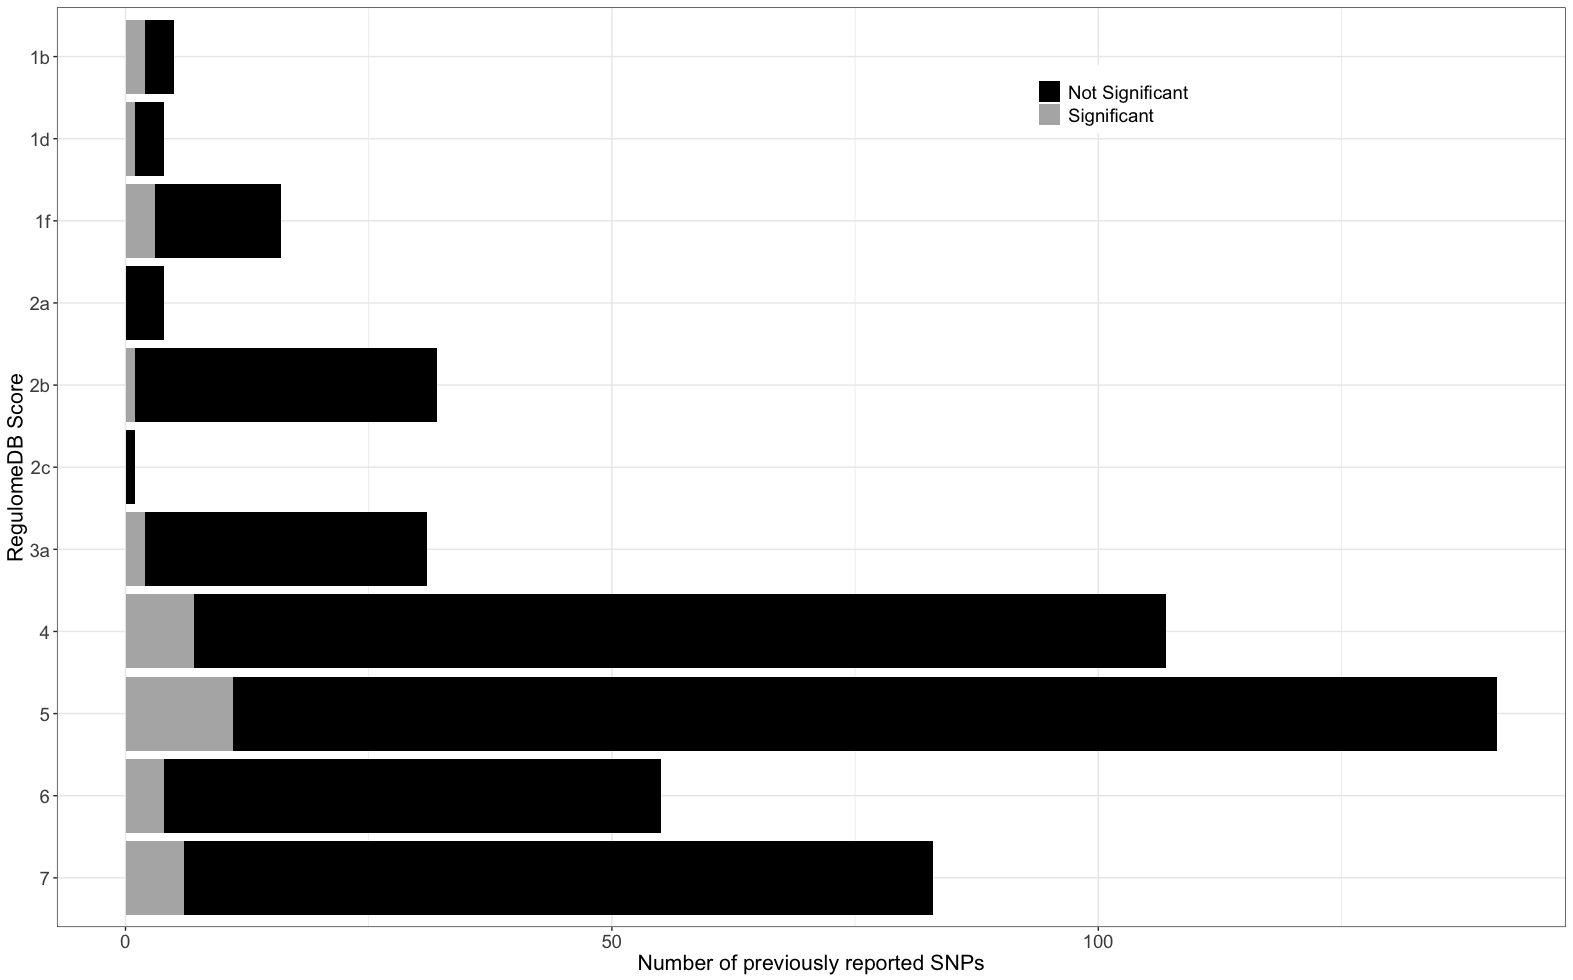
\includegraphics[width=\linewidth, height=3.5in]{~/Desktop/figures/chapter2/regulomedb_assoc.png}
    \caption[RegulomeDB score distribution of previously studied polymorphisms.]{RegulomeDB score distribution of previously studied polymorphisms. RegulomeDB categories are shown on the x-axis; counts of SNPs falling into RegulomeDB score category are shown on the y-axis. Blue portion of the bar indicates the counts of SNPs that were tested but not reported significant; red portion shows the counts of SNPs that were reported significant at least once. Score descriptions are given below the image. 1b indicates eQTL 1 transcription factor (TF) binding 1 any motif 1 DNase footprint 1 DNase peak; 1d, eQTL 1 TF binding 1 any motif 1 DNase peak; 1f, eQTL 1 TF binding/DNase peak; 2a, TF binding 1 matched TF motif 1 matched DNase footprint 1 DNase peak; 2b, TF binding 1 any motif 1 DNase footprint 1 DNase peak; 2c, TF binding 1 matched TF motif 1 DNase peak; 3a, TF binding 1 any motif 1 DNase peak; 4, TF binding 1 DNase peak; 5, TF binding or DNase peak; 6, motif hit; 7, no evidence.}
    \label{fig:regdb}
\end{figure}

Candidate gene SNPs were analyzed using the RegulomeDB, VEP and Blood
eQTL Browser databases to assess their functional characteristics and
better understand their biological framework. Eighty percent of
previously reported SNPs had RegulomeDB scores greater than 3 (Figure
\ref{fig:regdb}), indicating that these SNPs have minimal to no effect
on modifying transcription. This distribution aligns with the overall
distribution of SNPs in the genome, thus the candidate SNPS are not
enriched for their impact on gene expression or transcription factor
binding. Our replication and validation analyses includes 2 protein
coding variants, VEP shows that only, rs2066845 (SNP12) in
\emph{NOD2/CARD15}, is predicted to be damaging and disease causing.

We were interested in better understanding the biological framework of
candidate SNPs that had previously been identified. The candidate SNPs
were analyzed using RegulomeDB, Blood eQTL Browser, and VEP to assess
functional characteristics. The majority (\(\geq 80\%\)) candidate SNPs
had RegulomeDB scores greater than 3 (Figure \ref{fig:regdb}). This
indicates that the SNPs had minimal to no evidence of modifying DNA
transcription. The observed distribution coincides with the overall
distribution of SNPs in the genome. Therefore, from our point of view,
the candidate SNPs are not enriched in terms of impact on TF binding or
gene expression. VEP analyses revealed that the candidate SNPs in our
replication and validation analyses only included 2 protein coding
variants, and that rs2066845 (SNP12) in \emph{NOD2/CARD15} is predicted
to be damaging and disease causing (Karaesmen et al.
\protect\hyperlink{ref-Karaesmen_2017}{2017}).

We looked at the Blood eQTL browser to determine if the candidate SNPs
played a roll in \emph{cis} gene expression of the candidate genes.
Rough half (\(\approx 52\%\)) of the 171 genes that are included from
the literature search had at least one significant (probe level false
discovery rate, FDR \(< 0.05\)) \emph{cis}-eQTL. And when compared to
the entire genome, approximately 44\% of genes have blood \emph{cis}
eQTLs (FDR \(P<0.05\)). However, when we look at the the candidate SNPs,
only 13\% are blood \emph{cis}-eQTLs. So while blood eQTLs have indeed
been identified in these genes, the SNPs that previous literature
studied, were not the ones that affected expression. Furthermore, almost
half of the eQTLs in the CGAS are correlated with expression, they alter
expression in neighboring or nearby genes rather than the gene they are
located in. For example, rs7975232 (\emph{VDR}) is an eQTL for
\emph{SLC48A1} while the \emph{CTLA4} SNPs studied are eQTLs for
\emph{CD28} (Karaesmen et al.
\protect\hyperlink{ref-Karaesmen_2017}{2017}). The remaining eQTLs were
correlated with expression of the candidate gene of interest, but in
most cases, were also significant eQTLs for several other nearby genes
(Karaesmen et al. \protect\hyperlink{ref-Karaesmen_2017}{2017}).

\section{Discussion}\label{discussion-1}

In this study, we aimed to replicate or validate all existing CGAS
literature that investigated the relationship between non-HLA genetic
effects on survival after allogeneic HSCT (Karaesmen et al.
\protect\hyperlink{ref-Karaesmen_2017}{2017}). Considering that the main
purpose of CGAS is to select SNPs due to known function at the gene
level, we conducted single SNP analyses and gene-based analyses to
determine the joint effects of marginally associated SNPs within
candidate genes while considering the underlying genetic correlation
structure due to LD.

Donor rs1800795 in \emph{IL6} was the only association (OS) that was
able to be reproduced using DISCOVeRY-BMT (only in the validation set;
no candidate SNPs replicated). The original authors (Balavarca et al.
\protect\hyperlink{ref-balavarca_2015}{2015}) studied \emph{IL6} due to
its known immunological function, as well as the fact that two prior
studies reported significant associations in different phenotypes: to
GVHD (Cavet et al. \protect\hyperlink{ref-cavet_2001}{2001}) and chronic
hepatitis C virus therapy (Yee et al.
\protect\hyperlink{ref-yee_2009}{2009}). No evidence of an association
of rs1800795 at \(P < 0.05\) in DISCOVeRY-BMT with death due to GVHD
and/or infection (data not shown). Furthermore, rs1800795 is found in an
intronic region of \emph{IL6}, and has no effect on \emph{IL6}
expression or levels, but rather is an eQTL for two other nearby genes
(Arnold et al. \protect\hyperlink{ref-snipa}{2015}, GTEx Consortium
(\protect\hyperlink{ref-gtex}{2013})). We made an extra effort to
validate interesting CGAS findings, such as in \emph{CCR5} and the H1/H1
risk groups from McDermott et al. 2010. These associations were found in
the largest study we attempted to validate, as well as having samples
from CIBMTR (earlier years than DISCOVeRY-BMT), and the reported effects
started two years after HSCT. We were not able to validate these
associations with either outcome at \(P < 0.10\) (the threshold
McDermott 2010 used, Figure \ref{fig:val_fig}).

\emph{CTLA4} was another gene that was studied frequently (Table
\ref{tab:repval_table}), this gene is a good example of the
heterogeneity to studies of genetic polymorphisms in HSCT and may be a
plausible explanation of why were unable to reproduce any of the
previous associations. The SNP rs5742909 in \emph{CTLA4} was studied in
6 independent studies of HLA MRD-HSCT donor-recipient pairs. For donors,
rs5742909 was reported to be associated with DRM in a smaller study
(N=120). The lack of consistency between studies is apparent --
previously two \emph{CTLA4} SNPS, rs231775 and rs231774 were reported
associated in recipients for PFS (\(P=0.025\)) -- and before this study,
only 1 of 9 studies tried to validate these results. These SNPs are like
many candidate gene hypotheses such that they have not been tested in
the same genome for the same outcome in similar populations, and if they
have, the sample size is very small.

The inclusion criteria with respect to disease, donor relation, or to
differences in our endpoint of 1-year survival versus longer-term
survival could be attributed as to why previous results are not
reproducible. As previous genetic associations were hypothesized to be
independent of the underlying disease, one may expect that results
should be reproducible in a homogeneous patient populations such as
DISCOVeRY-BMT, which unfortunately was not the case. This study
meticulously attempted to align the study population in DISCOVeRY-BMT to
the original studies (i.e.~subset the full population for this only with
AML). DISCOVeRY-BMT primarily focuses on 1-year survival after HSCT and
this may have different genetic effects than later survival, however,
the survival curves from the CGAS often showed separation of death
occurring well into the first year. DISCOVeRY-BMT has a large sample
size that is adequately powered (L. E. Sucheston-Campbell et al.
\protect\hyperlink{ref-lsc_2015}{2015}) to reproduce results from
previously published CGAS. However, we were unable to reproduce almost
all of the findings. This is in agreement with other studies in this
field, Particularly in the context of death due to GVHD as an outcome
(Chien et al. \protect\hyperlink{ref-chien_2012}{2012}; Martin et al.
\protect\hyperlink{ref-martin_2016}{2016}). Several other reports have
also concluded that published CGAS have presented false positive
associations (Ioannidis et al.
\protect\hyperlink{ref-Ioannidis_2001}{2001}).

Confirmatory studies are vital to identify true positive genetic
variants that are associated to complex phenotypes. False positives may
lead researchers to allocate resources and time to research that will
lead to a dead end. In the long-term this may delay treatment to
patients or discovery of markers that would be relevant in improving
survival after HSCT. As only one SNP had a predicted damage or
deleterious effect and that a only a small proportion of the previous 70
studies conducted research on SNPs that correlated with gene expression,
we conclude that the transplant field can look agnostically at the
entire genome to hone in on potential candidate genes and SNPs
(Karaesmen et al. \protect\hyperlink{ref-Karaesmen_2017}{2017}). And
while we could not reproduce previous associations, the SNPs selected
are not linked to functional annotation nor are they clearly related to
the candidate genes. This underscores a fundamental flaw with CGAS which
are contingent on the scientific knowledge at the time. We assert that
by using adequately powered testing (i.e.~larger studies, GWAS) with
transplant will be vital to identifying promising targets and further
help us understand the underlying biological framework and how it
relates to survival outcomes, with the global objective of improving
patient outcomes (Karaesmen et al.
\protect\hyperlink{ref-Karaesmen_2017}{2017}).

\FloatBarrier

\newpage

\pagestyle{plain} \fancyhead[L]{} \fancyhead[R]{}
\fancyfoot[C]{\thepage}
\chapter{gwasurvivr: an R Bioconductor package for genome wide survival analysis}
\doublespacing

\section{Abstract}\label{abstract-1}

Summary: To address the limited software options for performing survival
analyses with millions of SNPs, we developed gwasurvivr, an
R/Bioconductor package with a simple interface for conducting
genome-wide survival analyses using VCF (outputted from Michigan or
Sanger imputation servers), IMPUTE2 or PLINK files. To decrease the
number of iterations needed for convergence when optimizing the
parameter estimates in the Cox model, we modified the R package
survival; covariates in the model are first fit without the SNP, and
those parameter estimates are used as initial points. We benchmarked
gwasurvivr with other software capable of conducting genome-wide
survival analysis (genipe, SurvivalGWAS\_SV and GWASTools). gwasurvivr
is significantly faster and shows better scalability as sample size,
number of SNPs and number of covariates increases.

Availability and implementation: gwasurvivr, including source code,
documentation and vignette are available at:
\url{http://bioconductor.org/packages/gwasurvivr}.

\section{Introduction}\label{introduction-2}

Genome-wide association studies (GWAS) are population-level experiments
that investigate genetic variation in individuals to observe single
nucleotide polymorphism (SNP) associations with a phenotype. Genetic
variants tested for association are genotyped on an array and imputed
from a reference panel of sequenced genomes using 1000 Genomes Project
or Haplotype Reference Consortium (HRC) (Das et al.
\protect\hyperlink{ref-michigan_imputation}{2016}; 1000 Genomes Project
Consortium \protect\hyperlink{ref-1000genomes}{2015}). Imputation
increases genome coverage from hundreds of thousands or a few million to
upwards of 30 million SNPs, improves power to detect genetic
associations, and/or homogenizes variant sets for meta-analyses (Das et
al. \protect\hyperlink{ref-michigan_imputation}{2016}). Imputed SNPs can
be tested for association with binary outcomes (case/control) and
quantitative outcomes (i.e.~height) using a range of available software
packages including SNPTEST (Marchini et al.
\protect\hyperlink{ref-snptest}{2007}) or PLINK (Purcell et al.
\protect\hyperlink{ref-plink}{2007}). Typically imputed SNPs are used in
association testing for large studies.

As we learned from our candidate gene replication/validation project,
researchers (including our lab) often opt to write custom survival
analysis scripts using the survival package in R. This hinders
reproducibility of results as unintentional errors may incur and
propagate without effectively testing and/or reviewing the custom
scripts. A solution to this would be a well-developed, flexible, and
tested open source software package that performs survival analysis on
GWAS data. Software options for performing survival analyses do indeed
exist, such as, genipe (Lemieux Perreault et al.
\protect\hyperlink{ref-genipe}{2016}), SurvivalGWAS\_SV (Syed,
Jorgensen, and Morris \protect\hyperlink{ref-survivalgwas_sv}{2017}), or
GWASTools (S. M. Gogarten et al.
\protect\hyperlink{ref-gwastools}{2012}). These software are able to
analyze millions of imputed SNPs but either require user interaction
with raw output, were not initially designed for survival and/or have
other limitations that could deter more introductory users (i.e.~mapping
patient meta data with the genetic data). To address these needs, we
developed an R/Bioconductor package, gwasurvivr, for genome wide
survival analyses of imputed data in multiple formats with flexible
analysis and output options (A. A. Rizvi et al.
\protect\hyperlink{ref-Rizvi_2018}{2018}). This package uses output from
the most popular imputation software and/or services as input, and
unlike other packages, no additional data wrangling or file format
conversion is needed. And then we wanted to test our package and compare
it to the other packages.

We wanted our package to perform and fulfill the following tasks:

\begin{itemize}
    \item User friendly 
    \item Propagate reproducible results
    \item Handle typed or imputed genetic data from common formats 
    \item Scalable for very large datasets
    \item Allow exploration of covariates when modeling 
    \item Interaction modeling, i.e. SNP $\times$ drug, SNP $\times$ age
    \item Compression of genetic data for less storage and faster computation
\end{itemize}

\section{Methods}\label{methods-1}

We detail our methodology and computational experiments conducted in the
development of gwasurvivr. This also includes generation of the
simulated data, survival analysis benchmarking and diagnostics. All of
the code that was published can be found in the
\href{https://github.com/suchestoncampbelllab/gwasurvivr_manuscript}{gwasurvivr
manuscript repository}. \href{https://git-lfs.github.com/}{GitHub Large
File Storage (LFS)} is on GitHub Large File Storage (LFS) or in the
\href{https://github.com/aarizvi/dissertation/tree/master/code/chapter3}{Appendix
GitHub}.

The repository can be cloned by invoking the following command:

\singlespacing

\begin{verbatim}
git lfs clone \    
    https://github.com/suchestoncampbelllab/gwasurvivr_manuscript.git
\end{verbatim}

\doublespacing

\subsection{Data Structure}\label{data-structure}

In a typical GWAS pipeline, raw genotyping data (`typed' data) is
pre-processed with standard quality control (QC)/quality assurance (QA)
and then delivered in PLINK (Purcell et al.
\protect\hyperlink{ref-plink}{2007}) formatted files (\texttt{.bed},
\texttt{.bim}, and \texttt{.fam} files). The primary representation of
the genotype calls are \texttt{.bed} files. \texttt{Bim} files are a
text file with no header containing more information about the variant
(chromosome, identified, position, base pair, and allele1 and allele2).
The \texttt{.fam} file contains information about the samples (family
ID, within-family ID, father ID, mother ID, sex code, and additional
phenotype information). PLINK does not do survival analysis to test for
association on its own and separate packages are needed.
\texttt{Gwasurvivr} was designed to take PLINK ready files directly
using \texttt{plinkCoxSurv}. For all survival analyses implemented in
\texttt{gwasurvivr}, in addition to the genetic data, a phenotype file
is needed, which contains survival time, survival status and additional
covariates, both files are indexed by sample ID. Potential data
wrangling that the user may have to do, however, is that they must
convert categorical variable need to be convert to indicator (or dummy)
variables and be class numeric (or integer).

Most GWAS, including DISCOVeRY-BMT, impute the typed data to obtain a
greater number of SNPs for association testing. In preparation for
imputation, PLINK files need to be converted into an appropriate format
(genotype (\texttt{.gen}) format for IMPUTE2 or VCF for Sanger and
Michigan imputation servers). The output format from these imputation
programs is the same as the input format (i.e.~VCF input, VCF output).
After imputation, the VCF files contain both sample IDs and imputation
quality metrics (INFO score {[}Sanger{]} or \(r^2\) {[}Michigan{]}),
while IMPUTE2 (B. N. Howie, Donnelly, and Marchini
\protect\hyperlink{ref-Howie_2009}{2009}) come in separate files
(\texttt{.gen}, \texttt{.sample}, and \texttt{.info}). Data from each
format are prepared in \texttt{gwasurvivr} by leveraging existing
Bioconductor packages GWASTools (S. M. Gogarten et al.
\protect\hyperlink{ref-gwastools}{2012}), VariantAnnotation (Obenchain
et al. \protect\hyperlink{ref-variantannotation}{2014}), or SNPRelate
(Zheng et al. \protect\hyperlink{ref-snprelate}{2012}) depending on the
imputation/typed data file format.

IMPUTE2 (B. N. Howie, Donnelly, and Marchini
\protect\hyperlink{ref-Howie_2009}{2009}) format is a standard genotype
(\texttt{.gen}) file which store genotype probabilities (GP). We
utilized GWASTools in R to compress files into genomic data structure
(GDS) format (S. M. Gogarten et al.
\protect\hyperlink{ref-gwastools}{2012}). GDS format compresses large
array-oriented datasets and allows for efficient, iterative access to
subsets of the data, while simultaneously converting GP into dosages
(DS) for use in survival analyses. The INFO score for IMPUTE2 (B. N.
Howie, Donnelly, and Marchini \protect\hyperlink{ref-Howie_2009}{2009})
results are not calculated in \texttt{gwasurvivr} internally, instead we
use the INFO scores that are provided in a separate file after
performing imputation (\texttt{.info} file). Users select SNPs from the
\texttt{.info} file to remove based on preferred criterion (i.e.~INFO
\textless{} 0.8) these are then used in the argument
\texttt{exclude.snps} in \texttt{impute2CoxSurv} to filter out the SNPs
prior to analysis. VCF files generated from these Michigan or Sanger
servers include a DS field and server-specific meta-fields (INFO score
{[}Sanger{]} or \(r^2\) {[}Michigan{]}, as well as reference panel
allele frequencies) that are iteratively read in by VariantAnnotation
(Obenchain et al. \protect\hyperlink{ref-variantannotation}{2014}). For
the Michigan imputation server, imputation is performed using the
minimac3 algorithm (Das et al.
\protect\hyperlink{ref-michigan_imputation}{2016}). minimac3 computes
and outputs an imputation quality metric known as \(R^2\). \(R^2\) is
the estimated value of the squared correlation between imputed genotypes
and true, unobserved genotypes (Das et al.
\protect\hyperlink{ref-michigan_imputation}{2016}). The \(R^2\) value is
extracted directly from the Michigan imputation output VCF in
\texttt{michiganCoxSurv}. For the Sanger imputation server, we extract
the INFO field directly from the VCF file in \texttt{sangerCoxSurv}. The
INFO field is the IMPUTE2 (B. N. Howie, Donnelly, and Marchini
\protect\hyperlink{ref-Howie_2009}{2009}) score as calculated by from
posterior genotype probabilities using bcftools + impute-info plugin
(McCarthy et al. \protect\hyperlink{ref-hrc}{2016}).

The \texttt{gwasurvivr} functions for IMPUTE2 (\texttt{impute2CoxSurv}
or \texttt{gdsCoxSurv}) and VCF (\texttt{michiganCoxSurv} or
\texttt{sangerCoxSurv}) include arguments for the survival model (event
of interest, time to event, and covariates) and arguments for quality
control that filter on minor allele frequency (MAF) or imputation
quality (michiganCoxSurv and sangerCoxSurv only). INFO score filtering
using \texttt{impute2CoxSurv} can be performed by accessing the
\texttt{.info} file from IMPUTE2 results and subsequently providing the
list of SNPs to \texttt{exclude.snps} argument to gwasurvivr. Users can
also provide a list of sample IDs for gwasurvivr to internally subset
the data. \texttt{Gwasurvivr} outputs two files:\\
(1) \texttt{.snps\_removed} file, listing all SNPs that failed QC
parameters\\
(2) \texttt{.coxph} file with the results from the analyses, including
parameter estimates, p-values, MAF, the number of events and total
sample \(N\) for each SNP.

Users can keep compressed GDS files after the initial run by setting
\texttt{keepGDS=TRUE} when using \texttt{impute2CoxSurv}. On subsequent
runs, \texttt{gdsCoxSurv} can then be used instead of
\texttt{impute2CoxSurv} to avoid compressing the data on each GWAS run.
This allows users to easily perform association testing on different
subsets of data as well.

\subsection{MAF Calculation}\label{maf-calculation}

After imputation, many SNPs will have low allele frequencies, as newer
imputation methods are able to impute SNPs with MAFs around 0.1\%
(McCarthy et al. \protect\hyperlink{ref-hrc}{2016}). As rare variant
analysis is beyond the scope of \texttt{gwasurvivr} and its usage is
only meant for common variant (MAF \textgreater{} 0.1\%) association
testing. \texttt{Gwasurvivr} allows users to filter out SNPs with low
MAFs. As such, we found it useful to calculate a MAF for each SNP
specifically for the samples that are being analyzed, and that
calculation is described below:

For a given SNP with alleles \(A\) and \(B\), where \(n_{AB}\) and
\(n_{BB}\) are the number of individuals with \(AB\) and \(BB\) genotype
respectively, and \(N\) is the sample size, the expected allele
frequency of allele \(B\) (\(freq_B\)) be can be calculated as:

\begin{equation} \label{1}
freq_B =  \frac{ n_{AB} + 2n_{BB}}{2N}
\end{equation}

\noindent For individual \(i\), the allele dosage of SNP \(j\)
(\(D_{ij}\)) with alleles \(A\) and \(B\), where allele \(B\) is the
effect allele and \(p_{AB}\) and \(p_{BB}\) are the posterior genotype
probabilities as computed by the imputation, is calculated as:

\begin{equation} \label{2}
D_{ij} = p_{AB_{ij}} + 2 \cdot p_{BB_{ij}}
\end{equation}

\noindent For SNP \(j\) The estimated allele frequency of an effect
allele \(B\) (\(\theta_{B_j}\)) can therefore be calculated as:

\begin{equation} \label{3}
\theta_{B_j} = \frac{\sum_{i=1}^{N} D_{ij} }{2N}
\end{equation}

\noindent In R, the genotypes are represented as a matrix allele
dosages, where each column is a sample and each row is a SNP. The R code
is shown below:

\singlespacing

\begin{Shaded}
\begin{Highlighting}[]
\KeywordTok{library}\NormalTok{(matrixStats)}
\NormalTok{exp_freq_A1 <-}\StringTok{ }\KeywordTok{round}\NormalTok{(}\KeywordTok{rowMeans2}\NormalTok{(genotypes) }\OperatorTok{*}\StringTok{ }\FloatTok{0.5}\NormalTok{, }
    \DecValTok{4}\NormalTok{)}
\NormalTok{MAF <-}\StringTok{ }\KeywordTok{ifelse}\NormalTok{(exp_freq_A1 }\OperatorTok{>}\StringTok{ }\FloatTok{0.5}\NormalTok{, }\DecValTok{1} \OperatorTok{-}\StringTok{ }\NormalTok{exp_freq_A1, }
\NormalTok{    exp_freq_A1)}
\end{Highlighting}
\end{Shaded}

\doublespacing 

\subsection{Modifying survival
package}\label{modifying-survival-package}

\texttt{Gwasurvivr} implements a Cox proportional hazards regression
model (Cox \protect\hyperlink{ref-cox1972}{1972}) to test each SNP with
an outcome with options for including covariates and/or SNP-covariate
interactions. As an early proof of principal in the development of
\texttt{gwasurvivr}, we assessed if we could speed up the survival
package during the parameter estimation step of the Cox model by
providing initial estimates covariates. Using the survival function as
implemented in the survival package improves computational time, we
tested a dataset of 500 individuals at 7255 SNPs with 1, 2, or 3
covariates. These data were simulated using HAPGENv2 (Su, Marchini, and
Donnelly \protect\hyperlink{ref-hapgen2}{2011}) and described in a
subsequent subsection ``Simulating Genotypes and Phenotypes''.

The helper function \texttt{gwasurvivr:::coxParam}, adjusted for this
demonstration in this document is labeled \texttt{gcoxph}. In
\href{https://github.com/suchestoncampbelllab/gwasurvivr_manuscript/blob/master/supplemental_data/code/gcoxph_model.R}{\texttt{gcoxph\_model.R}}
we fit the model without the SNP and the parameter estimates are then
used as initial points for all subsequent models and applied over all
SNPs in the dataset (See
\href{https://github.com/suchestoncampbelllab/gwasurvivr_manuscript}{manuscript
GitHub} or
\href{https://github.com/aarizvi/dissertation/tree/master/code/chapter3}{Dissertation
GitHub}). To decrease the number of iterations needed for convergence
when optimizing the parameter estimates in the Cox model we modified the
R package survival and function \texttt{survival::coxph.fit} (Therneau
and Grambsch \protect\hyperlink{ref-therneau2013}{2013}). Covariates in
the model are first fit without the SNP, and those parameter estimates
are used as initial points for analyses with each SNP. If no additional
covariates are added to the model, the parameter estimation optimization
begins with null initial value. This is implemented in gwasurvivr by
manually creating the objects found in the helper function
(\texttt{survival::coxph.fit}) that fits the Cox model. These R objects
and object descriptions can be see in (Table 3.1). These variables are
then passed to \texttt{survival::coxph.fit} (essentially the purpose of
\texttt{gwasurvivr:::coxParam} function).

\begin{table}[t]

\caption{\label{tab:unnamed-chunk-27}Description of arguments that are built manually in gwasurvivr and passed directly to survival::coxph.fit, bypassing the main survival::coxph function}
\centering
\fontsize{9}{11}\selectfont
\begin{tabular}{ll}
\toprule
variables & description\\
\midrule
X & matrix of predictors\\
Y & Surv object\\
STRATA & vector containing stratification, we set to NULL\\
OFFSET & offset vector, we set to NULL\\
INIT & initial values for coefficients\\
\addlinespace
CONTROL & result of a call to survival:::coxph.control\\
WEIGHTS & vector of weights that we set to NULL\\
METHOD & efron method used for handling ties\\
ROWNAMES & rownames that we set to NULL\\
\bottomrule
\end{tabular}
\end{table}

The function
\href{https://github.com/suchestoncampbelllab/gwasurvivr_manuscript/blob/master/supplemental_data/code/coxph_model.R}{\texttt{coxph\_model.R}}
implements a \texttt{survival} model (survival package, Therneau and
Grambsch \protect\hyperlink{ref-therneau2013}{2013}) without using the
optimization starting point obtained from including covariates in the
model. To test the package runtime over a pre-specified number of
iterations and including 1, 2, or 3 covariates the
\texttt{microbenchmark} package (Mersmann
\protect\hyperlink{ref-microbenchmark}{2018}) in R was used.

In order to maximize compute, \texttt{parallel::parApply} (R Core Team
\protect\hyperlink{ref-r_core}{2018}) was used instead of
\texttt{base::apply} (R Core Team \protect\hyperlink{ref-r_core}{2018}).
The number of cores used during computation on Windows and Linux can be
specified by the user.

\doublespacing 

\subsection{Computational Experiments}\label{computational-experiments}

Upon completion of \texttt{gwasurvivr}, we wanted to compare
functionality and runtime with other available GWAS survival packages,
specifically GWASTools, SurvivalGWAS\_SV and genipe. None of these other
packages directly take VCF data output from Sanger or Michigan
imputation servers. SurvivalGWAS\_SV does accept VCF files as an input
but uncompressed and not explicity the same format that Sanger and
Michigan imputation servers output, rendering additional steps to be
taken. Thus, the computational experiments comprised simulated genetic
data were formatted as output from IMPUTE2 software (\texttt{.gen}).
Computational runtimes for gwasurvivr were benchmarked against existing
software comparing varying sample sizes and SNP numbers, increasing
covariates, for a single chromosome with ranging 15,000-25,000
individuals. In addition, we evaluated time for \texttt{gwasurvivr} for
a complete GWAS (\textasciitilde{}6 million SNPS) for 3000, 6000 and
9000 samples.

\subsubsection{Simulating Genotypes and
Phenotypes}\label{simulating-genotypes-and-phenotypes}

\href{http://mathgen.stats.ox.ac.uk/genet\%20dics_software/hapgen/hapgen2.html}{HAPGENv2}
(Su, Marchini, and Donnelly \protect\hyperlink{ref-hapgen2}{2011}) was
used to generate simulated genotype datasets from
\href{https://mathgen.stats.ox.ac.uk/impute/impute_v1.html\#Using_IMPUTE_with_the_HapMap_Data}{1000
Genomes Project CEU data} (NCBI Build 36) (1000 Genomes Project
Consortium \protect\hyperlink{ref-1000genomes}{2015}) for all
benchmarking experiments. To replicate simulations the 1000 Genomes
Project CEU data should be downloaded in its entirety.

For each sample size tested, survival events (alive/dead) were simulated
as two separate datasets. For the dead dataset, time to event and
covariates were simulated using a normal distribution. For the alive
dataset, time was simulated by randomly sampling weighted probabilities
for times to simulate few samples being censored, covariates were
simulated from a normal distribution. Principal components (Zheng et al.
\protect\hyperlink{ref-snprelate}{2012}) were simulated using random
normal distributions with decreasing variance for each additional PC.
Furthermore, the \texttt{.sample} file from IMPUTE2 includes 4 columns
(ID\_1, ID\_2, missing, and sex) which link individuals with their
respective genotypes. For SurvivalGWAS\_SV and GWASTools, the simulated
phenotypes were appended to column 5 onward in the \texttt{.sample}
file. The code for all of these analyses is available (or linked to) in
the
\href{https://github.com/aarizvi/dissertation/tree/master/code/chapter3}{Appendix
GitHub} or from the
\href{https://github.com/suchestoncampbelllab/gwasurvivr_manuscript}{manuscript
GitHub}.

\subsubsection{Running analysis}\label{running-analysis}

We used the University at Buffalo Computational Center for Research (UB
CCR) academic cluster for our benchmarking analyses. Each analysis was
run exclusively on node
\href{https://www.buffalo.edu/ccr/support/research_facilities/general_compute.html}{CPU-L5520}
with the same system specifications, controlling the computational
resources for each run. The UB CCR uses Simple Linux Utility for
Resource Management (SLURM) scheduling for jobs. SLURM scripts to run
the analyses were generated using shell scripts below. Benchmarking was
performed using identical CPU constraints, 1 node (2.27 GHz Clock Rate)
and 8 cores with 24 GB of RAM, on the University at Buffalo Center for
Computational Research supercomputer. With the exception of the larger
sample size tests, these were run using the same node but 12 CPUs.
genipe (Lemieux Perreault et al. \protect\hyperlink{ref-genipe}{2016}),
SurvivalGWAS\_SV (Syed, Jorgensen, and Morris
\protect\hyperlink{ref-survivalgwas_sv}{2017}), and GWASTools (S. M.
Gogarten et al. \protect\hyperlink{ref-gwastools}{2012}) were performed
as specified by the authors on available online documentation.

We performed the following benchmarking simulations with varying sample
sizes (\(n\)) and SNP numbers (\(m\)):\\
\noindent \textbf{Simulation 1.} Compare \texttt{gwasurvivr} against
genipe, GWASTools and SurvivalGWAS\_SV - varying sample sizes
(\(n=100\), \(n=1000\), \(n=5000\)) and \(100,000\) SNPs (\(m=100,000\)
from chromosome 18) and 3 non-genetic covariates.\\
\noindent \textbf{Simulation 2.} Comparison of \texttt{gwasurvivr},
genipe, GWASTools and SurvivalGWAS\_SV with \(n=5,000\) and \(100,000\)
SNPs (\(m=100,000\)) with 4 covariates (age, drug treatment, sex and 1
PC), 8 covariates (age, drug treatment, sex and 5 PCs) and 12 covariates
(age, drug treatment, sex and 9 PCs).\\
\noindent \textbf{Simulation 3.} \texttt{gwasurvivr} runtime for
increasingly larger sample sizes (\(n=15,000\), \(20,000\) and
\(25,000\)) tested on chromosome 22.\\
\noindent \textbf{Simulation 4.} Full autosomal GWAS with varying sample
sizes using \texttt{gwasurvivr} (\(n=3,000\), \(n=6,000\) and
\(n=9,000\)).

Additionally, to maximize the performance of SurvivalGWAS\_SV, these
jobs were run using ``array'' jobs as recommended by the authors. An
\href{https://www.liverpool.ac.uk/media/livacuk/instituteoftranslationalmedicine/biostats/batchexample.sh}{example
batch script}, provided in the SurvivalGWAS\_SV documentation, was
converted from PBS to SLURM. 24GB of ram was not needed on all runs,
however was used to ensure each run remained uniform. The jobs were
split into array sets of 1000 SNPs for \(m=100,000\), totaling 100
batched jobs in a single array. Thus, we define \emph{rate-limiting
array} as the array index that had the longest runtime. This is an
important caveat and bears consideration when using SurvivalGWAS\_SV.
Depending on availability on the computing cluster, the analyses could
be completed as quickly as the longest individual array job, or
potentially the entire runtime could be equal to the summation runtime
of all of the array indices if these cannot be run simultaneously (or if
there are failures with any of the array indices).

Custom scripts were written in R or bash to streamline the analyses. For
\texttt{gwasurvivr} and GWASTools, a `run' script was used that involved
passing variables that were assigned in bash into R variables and
passing them into \texttt{gwasurvivr} or GWASTools within an R session.
Both genipe and SurvivalGWAS\_SV can be invoked directly from the
command line, so bash scripts were written to automate these processes
for the different experiments. Please see the
\href{https://github.com/aarizvi/dissertation/tree/master/code/chapter3}{Appendix
GitHub} or
\href{https://github.com/suchestoncampbelllab/gwasurvivr_manuscript}{manuscript
GitHub} for the code.

\section{Results}\label{results-1}

\begin{figure}
    \centering
    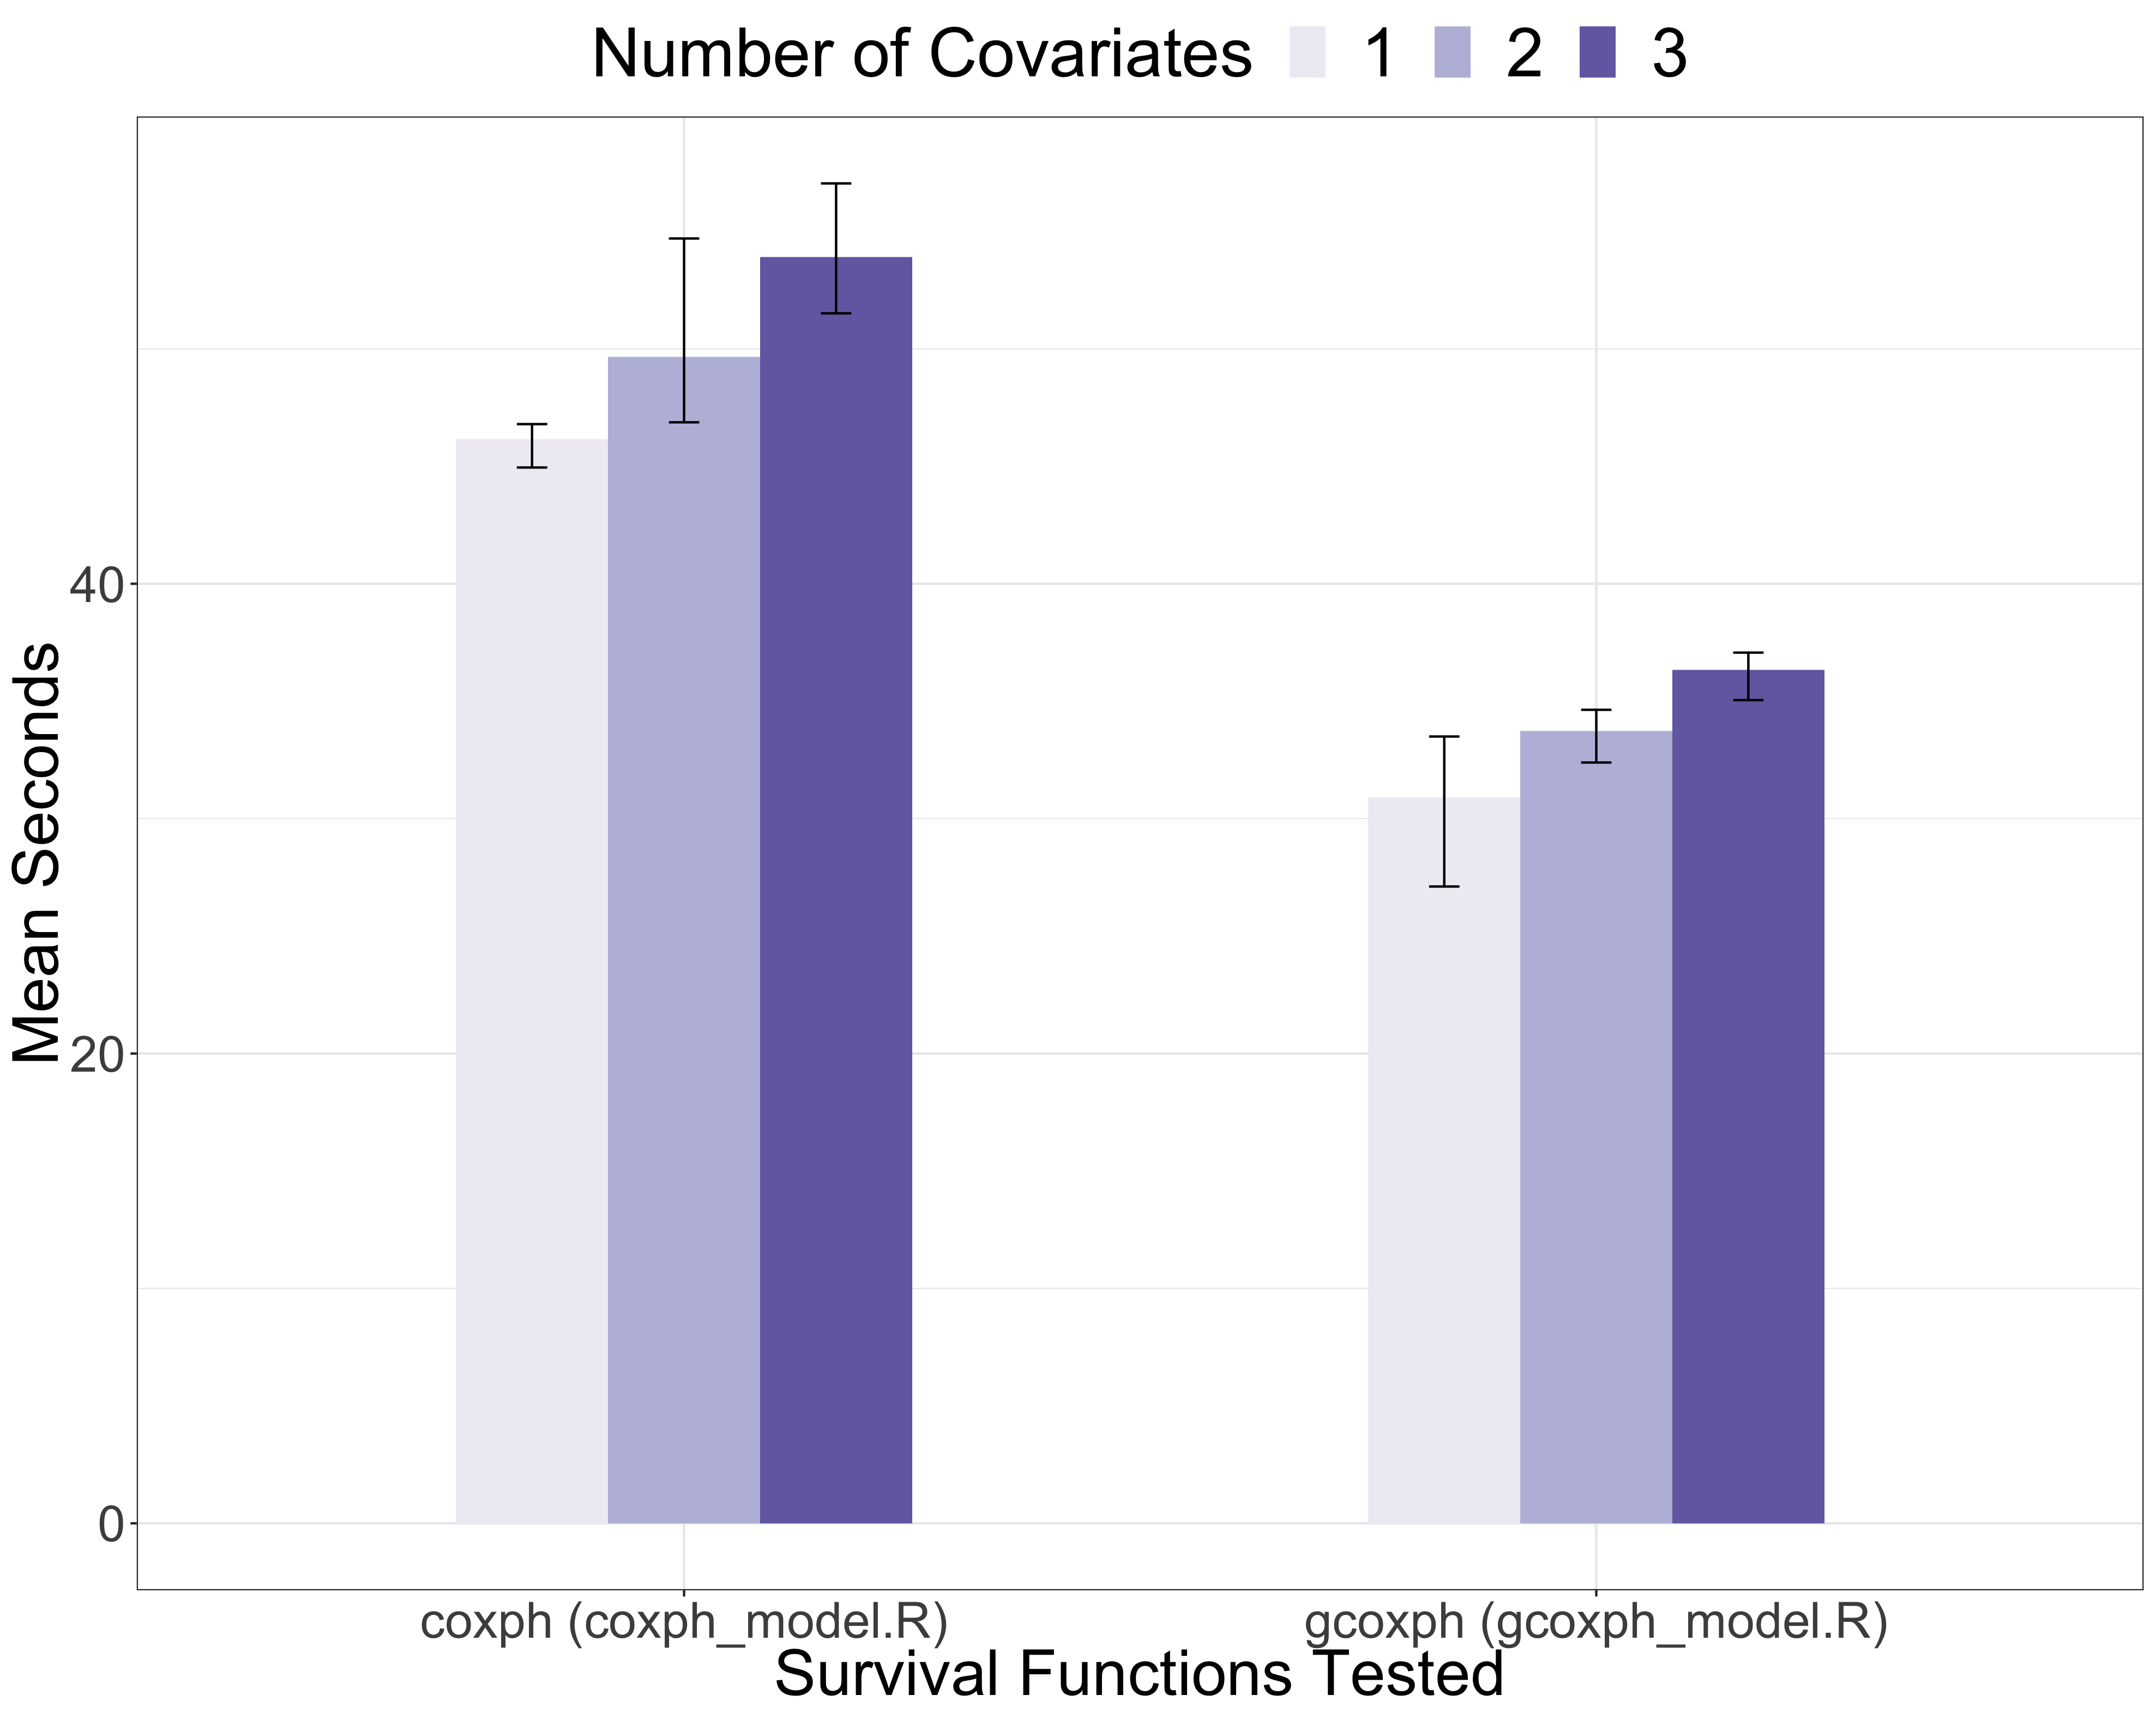
\includegraphics[width=\linewidth, height=4in]{~/Desktop/figures/chapter3/convergence_time_sim.png}
    \caption[Time to convergence of original R survival package implementation vs. modified implementation using simulated data.]{Time to convergence of original R survival package implementation vs modified implementation using simulated data. The x-axis are the survival functions tests, coxph and gcoxph. The y-axis are mean seconds from three iterations of each function. The error bars represent the maximum and minimum run time from three iterations with the barplots showing the mean runtimes of either coxph or gcoxph for 1, 2, or 3 covariates. gcoxph, which fits initial points based on parameter estimates from covariates alone, runs on average faster than the traditional coxph model for 1, 2, and 3 non-genetic covariates and shows a decreasing min to max range as the number of covariates increase.}  
    \label{fig:conv_plot}  
\end{figure}

\subsection{Cox Model Modifications}\label{cox-model-modifications}

Speeding up the original Cox model implemented in the survival package.
By leveraging an initalization point from the analyses with covariates
\texttt{gwasurvivr} (gcoxph) is several seconds faster than the survival
analyses function as implemented in \texttt{survival} (coxph, Therneau
and Grambsch (\protect\hyperlink{ref-therneau2013}{2013})) in R (Figure
\ref{fig:conv_plot}). While this is a small test dataset, in practice
this would be an appreciable difference when testing across several
thousands of samples and millions of SNPS.

\begin{figure}
    \centering
    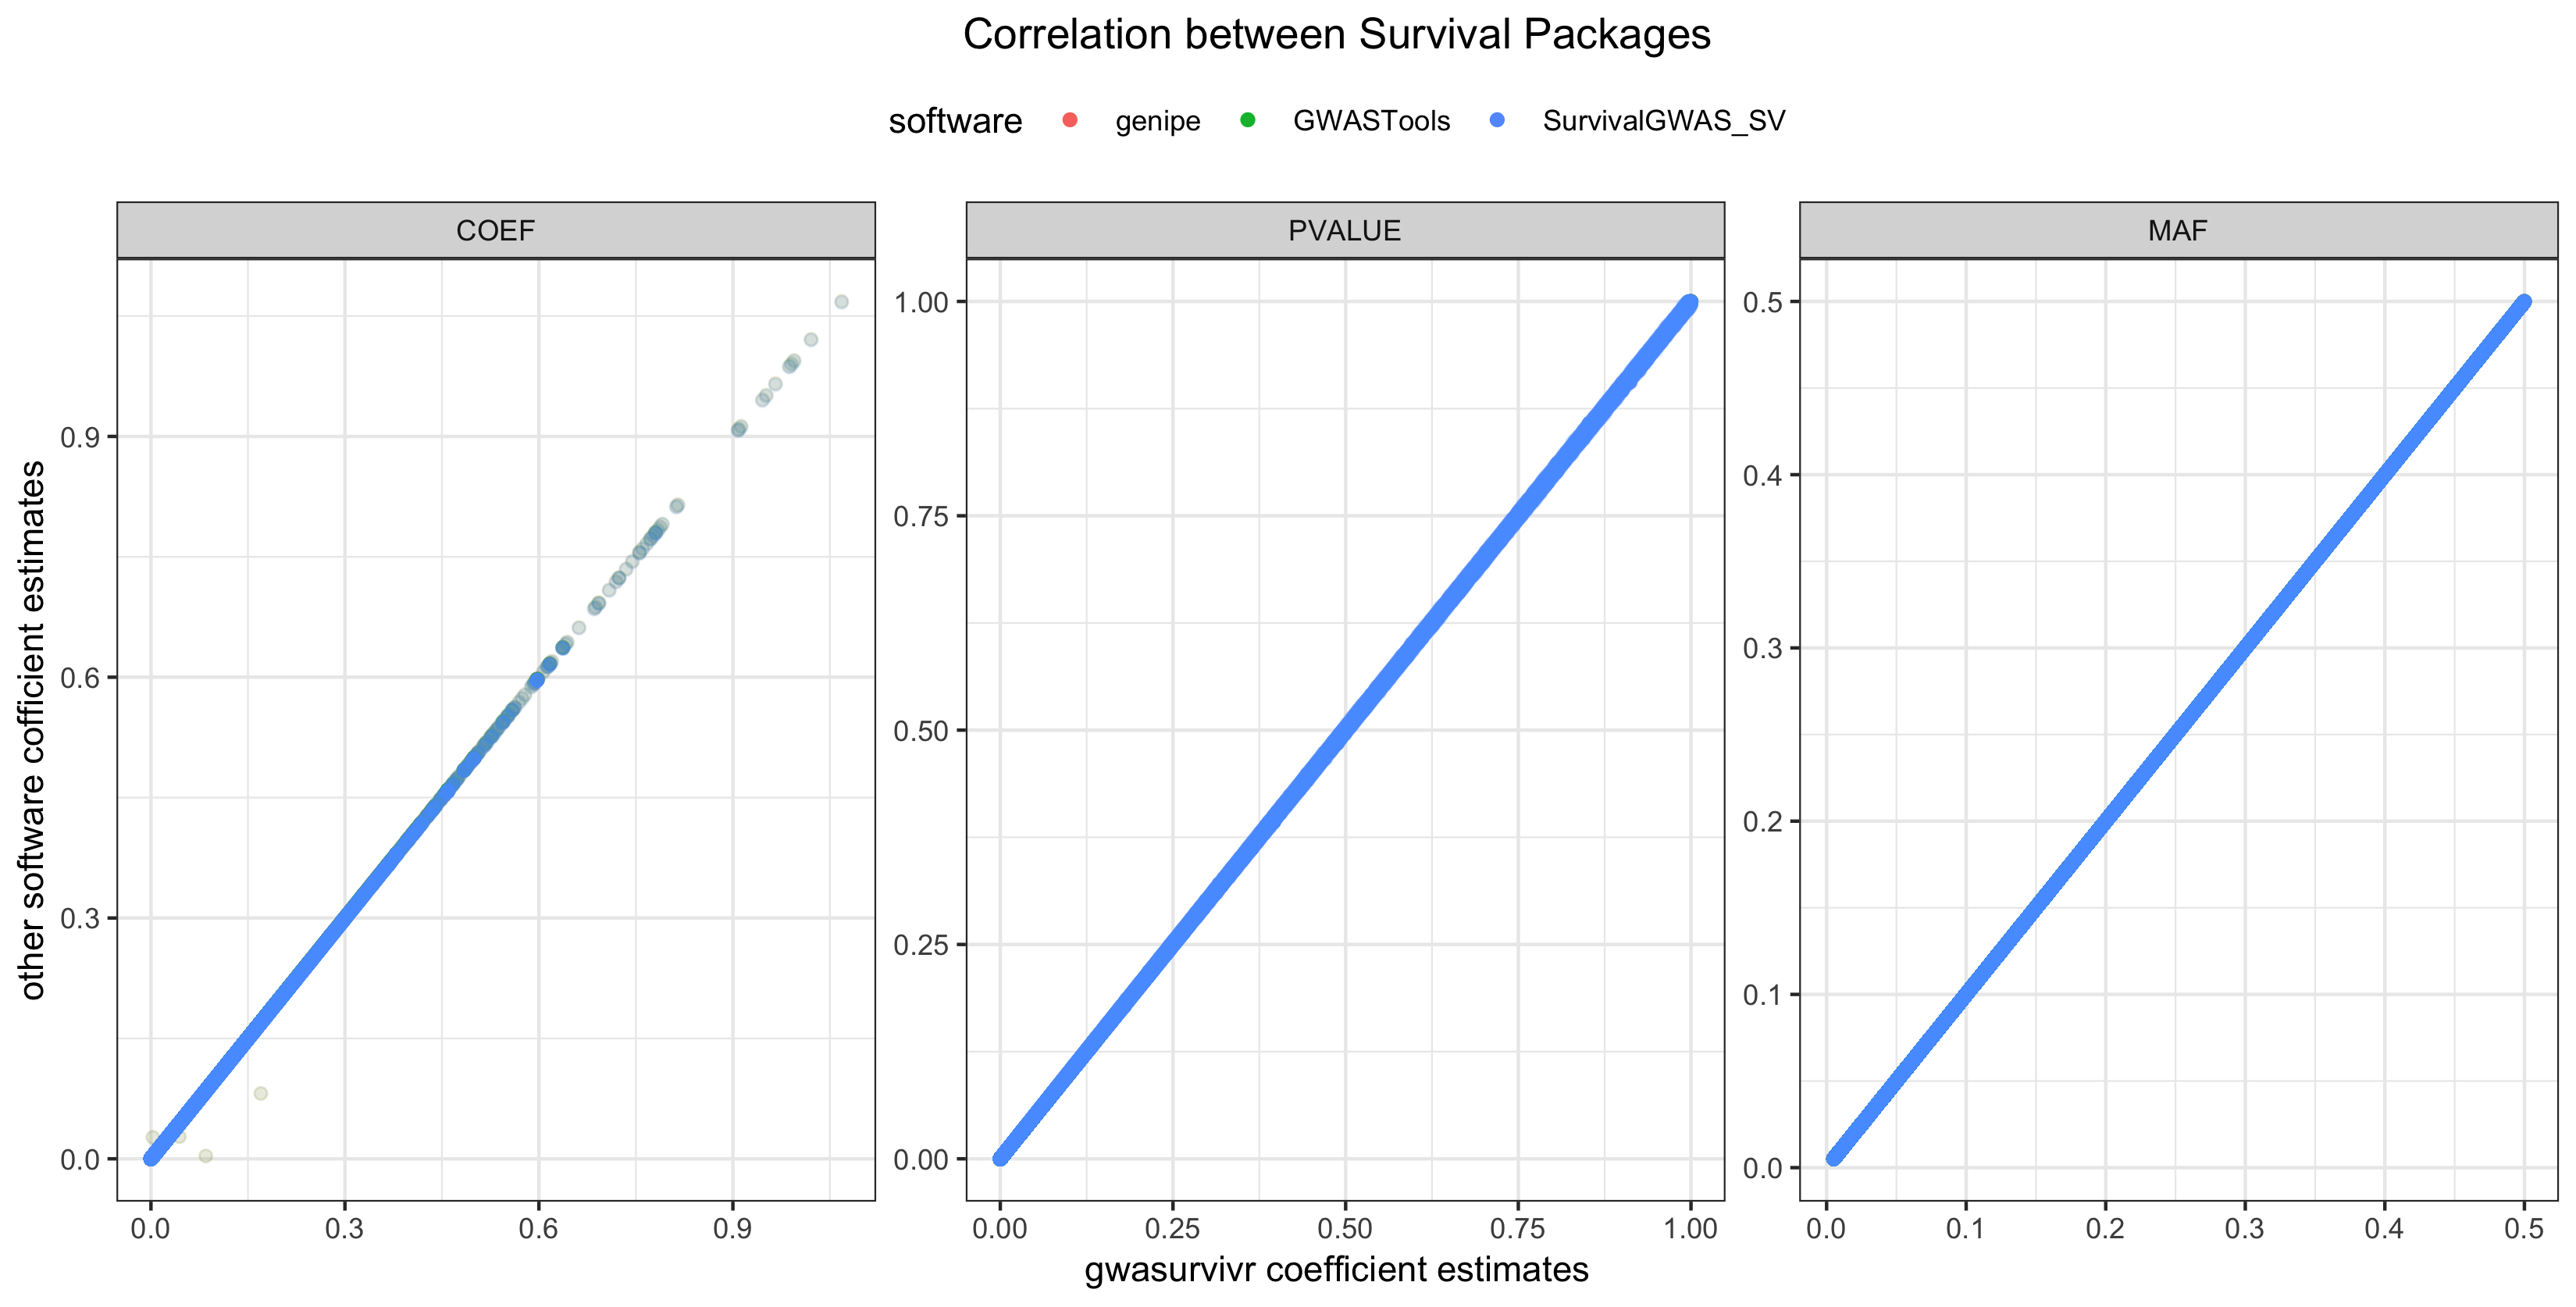
\includegraphics[width=\linewidth, height=2.5in]{~/Desktop/figures/chapter3/correlation_stats.png}
    \caption[Correlation of parameter estimates and minor allele frequency across survival analysis packages.]{Correlation of parameter estimates and minor allele frequency across survival analysis packages. Shown here are $n=5000$ and $m=100,000$. The x-axes (from left-to-right) are gwasurvivr coefficient estimates, pvalues, and minor allele frequency (MAF). The y-axes  (from left-to-right) are coefficient estimates, pvalues, and minor allele frequency (MAF) from the other software, respectively. The points are colored to indicate the software being used where red is genipe, green is GWASTools alone, and blue is SurvivalGWAS\_SV. The estimates are near perfectly correlated and thus not all colors are visible in each plot.}  
    \label{fig:corr_plot}  
\end{figure}

\subsection{Benchmarking Analyses}\label{benchmarking-analyses}

\subsubsection{Differing Sample Size Runtime: gwasurvivr vs.~other
software}\label{differing-sample-size-runtime-gwasurvivr-vs.other-software}

The computational benchmarking experiments comparing \texttt{gwasurvivr}
with genipe, GWASTools, and SurvivalGWAS\_SV were done using a sample
size of \(n=5,000\) and \(m=100,000\) SNPs. The coefficient estimates
from the Cox model and p-values are perfectly correlated between the
packages (Figure \ref{fig:corr_plot}, left and center panels). The
\texttt{gwasurvivr} sample MAF calculation (Equation \ref{3}) is
perfectly correlated with the MAFs calculated from the other software
(Figure \ref{fig:corr_plot}, right panel).

\begin{figure}
    \centering
    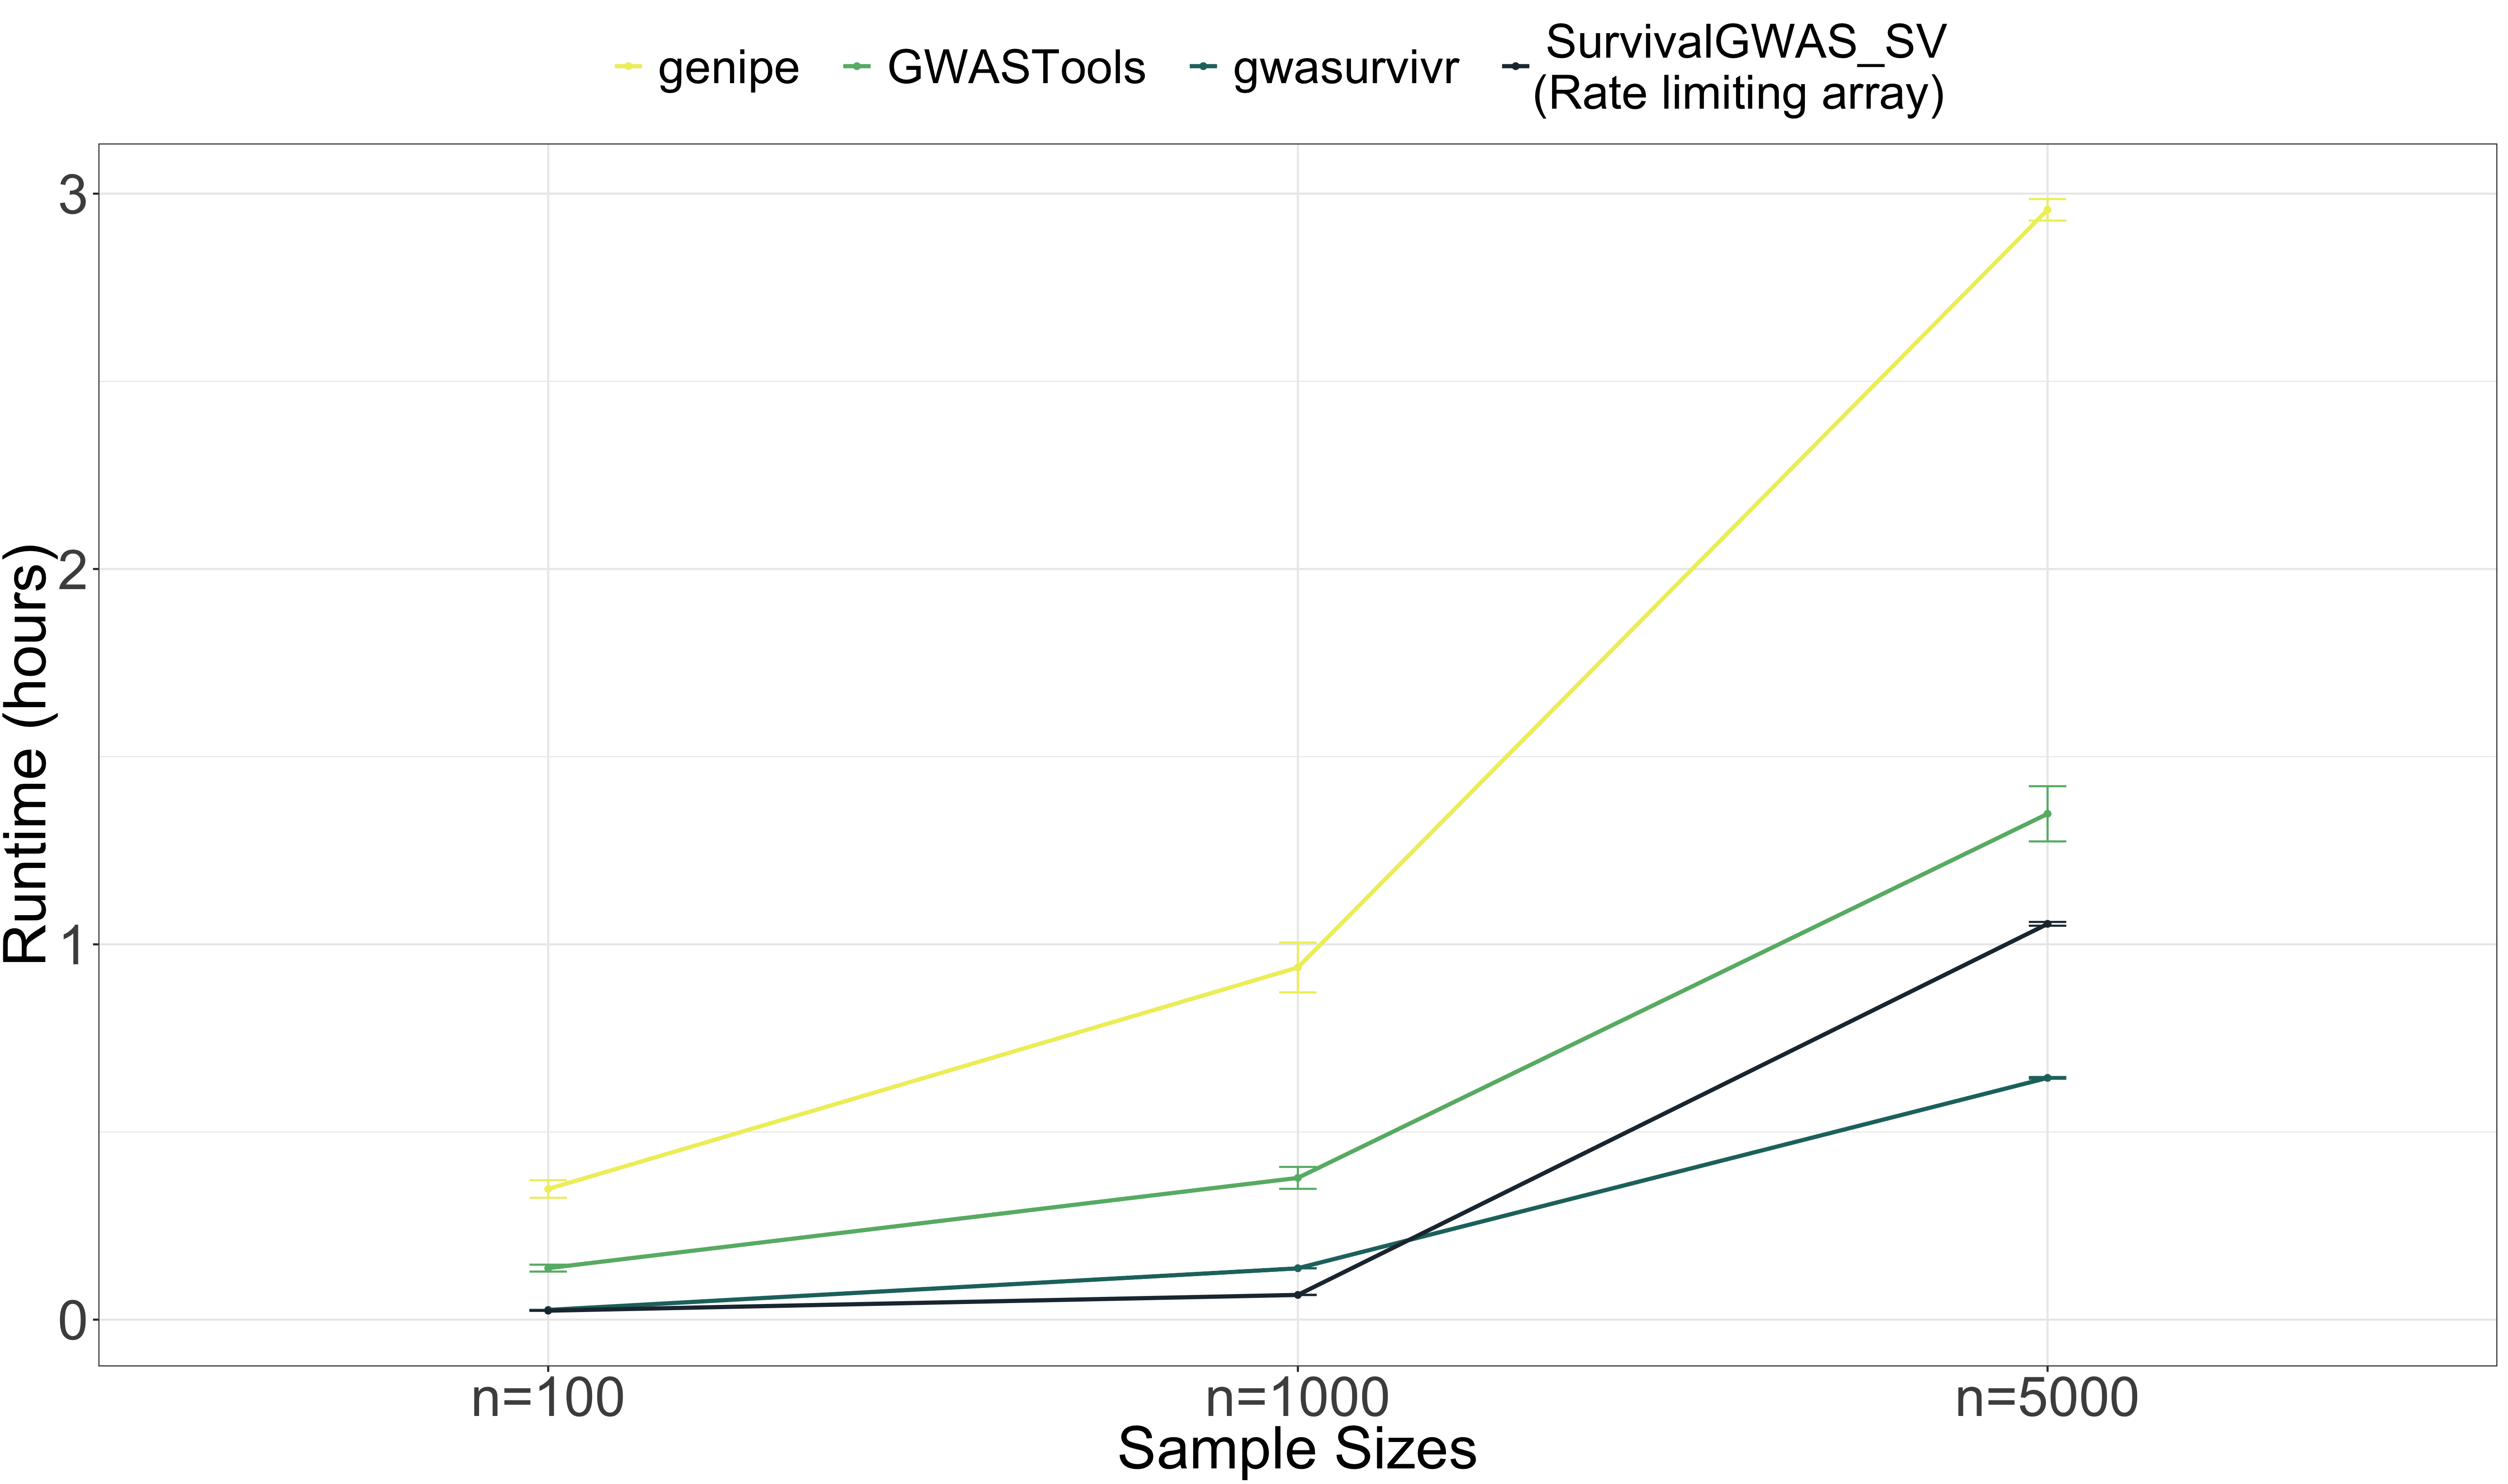
\includegraphics[width=\linewidth, height=3in]{~/Desktop/figures/chapter3/benchmarking_plot.png}
    \caption[Runtime for survival analyses between survival software.]{Runtime for survival analyses between different survival software. The x-axis shows the three sample sizes with 100,000 SNPs. The y-axis is the total runtime in hours. Mean and $95\%$ confidence intervals (CI) are show for genipe (yellow), GWASTools (light green), SurvivalGWAS\_SV (dark blue) and gwasurvivr (dark green). Confidence intervals were calculated for 3 simulations for each $n$ and $m$ combination.}  
    \label{fig:gwsfig1}  
\end{figure}

Scalability is a key component in software design, particularly in
contemporary times with growth of data. As such, we wanted to benchmark
how well \texttt{gwasurvivr} (and the other software) scaled as sample
size increased from \(n=100\), \(n=1000\), and \(n=5000\).
\texttt{gwasurvivr} was faster than genipe (Lemieux Perreault et al.
\protect\hyperlink{ref-genipe}{2016}), SurvivalGWAS\_SV (Syed,
Jorgensen, and Morris \protect\hyperlink{ref-survivalgwas_sv}{2017}),
and GWASTools (S. M. Gogarten et al.
\protect\hyperlink{ref-gwastools}{2012}) for \(m=100,000\) SNPs at
\(n=100\), and \(n=5000\), with the exception of SurvivalGWAS\_SV at
\(n=1000\) (Figure \ref{fig:gwsfig1}). To reiterate, the reported time
is the rate-limiting of SurvivalGWAS\_SV (the shortest runtime for 1 of
10 arrays), meaning this may not necessarily reflect on how quickly the
analysis will complete, as it could vary between one to all arrays.
\texttt{Gwasurvivr} is orders of magnitudes faster than the other
software when the sample size is \(n=5000\) (Figure \ref{fig:gwsfig1}).

\subsubsection{Increasing sample size tests with
gwasurvivr}\label{increasing-sample-size-tests-with-gwasurvivr}

\begin{figure}
    \centering
    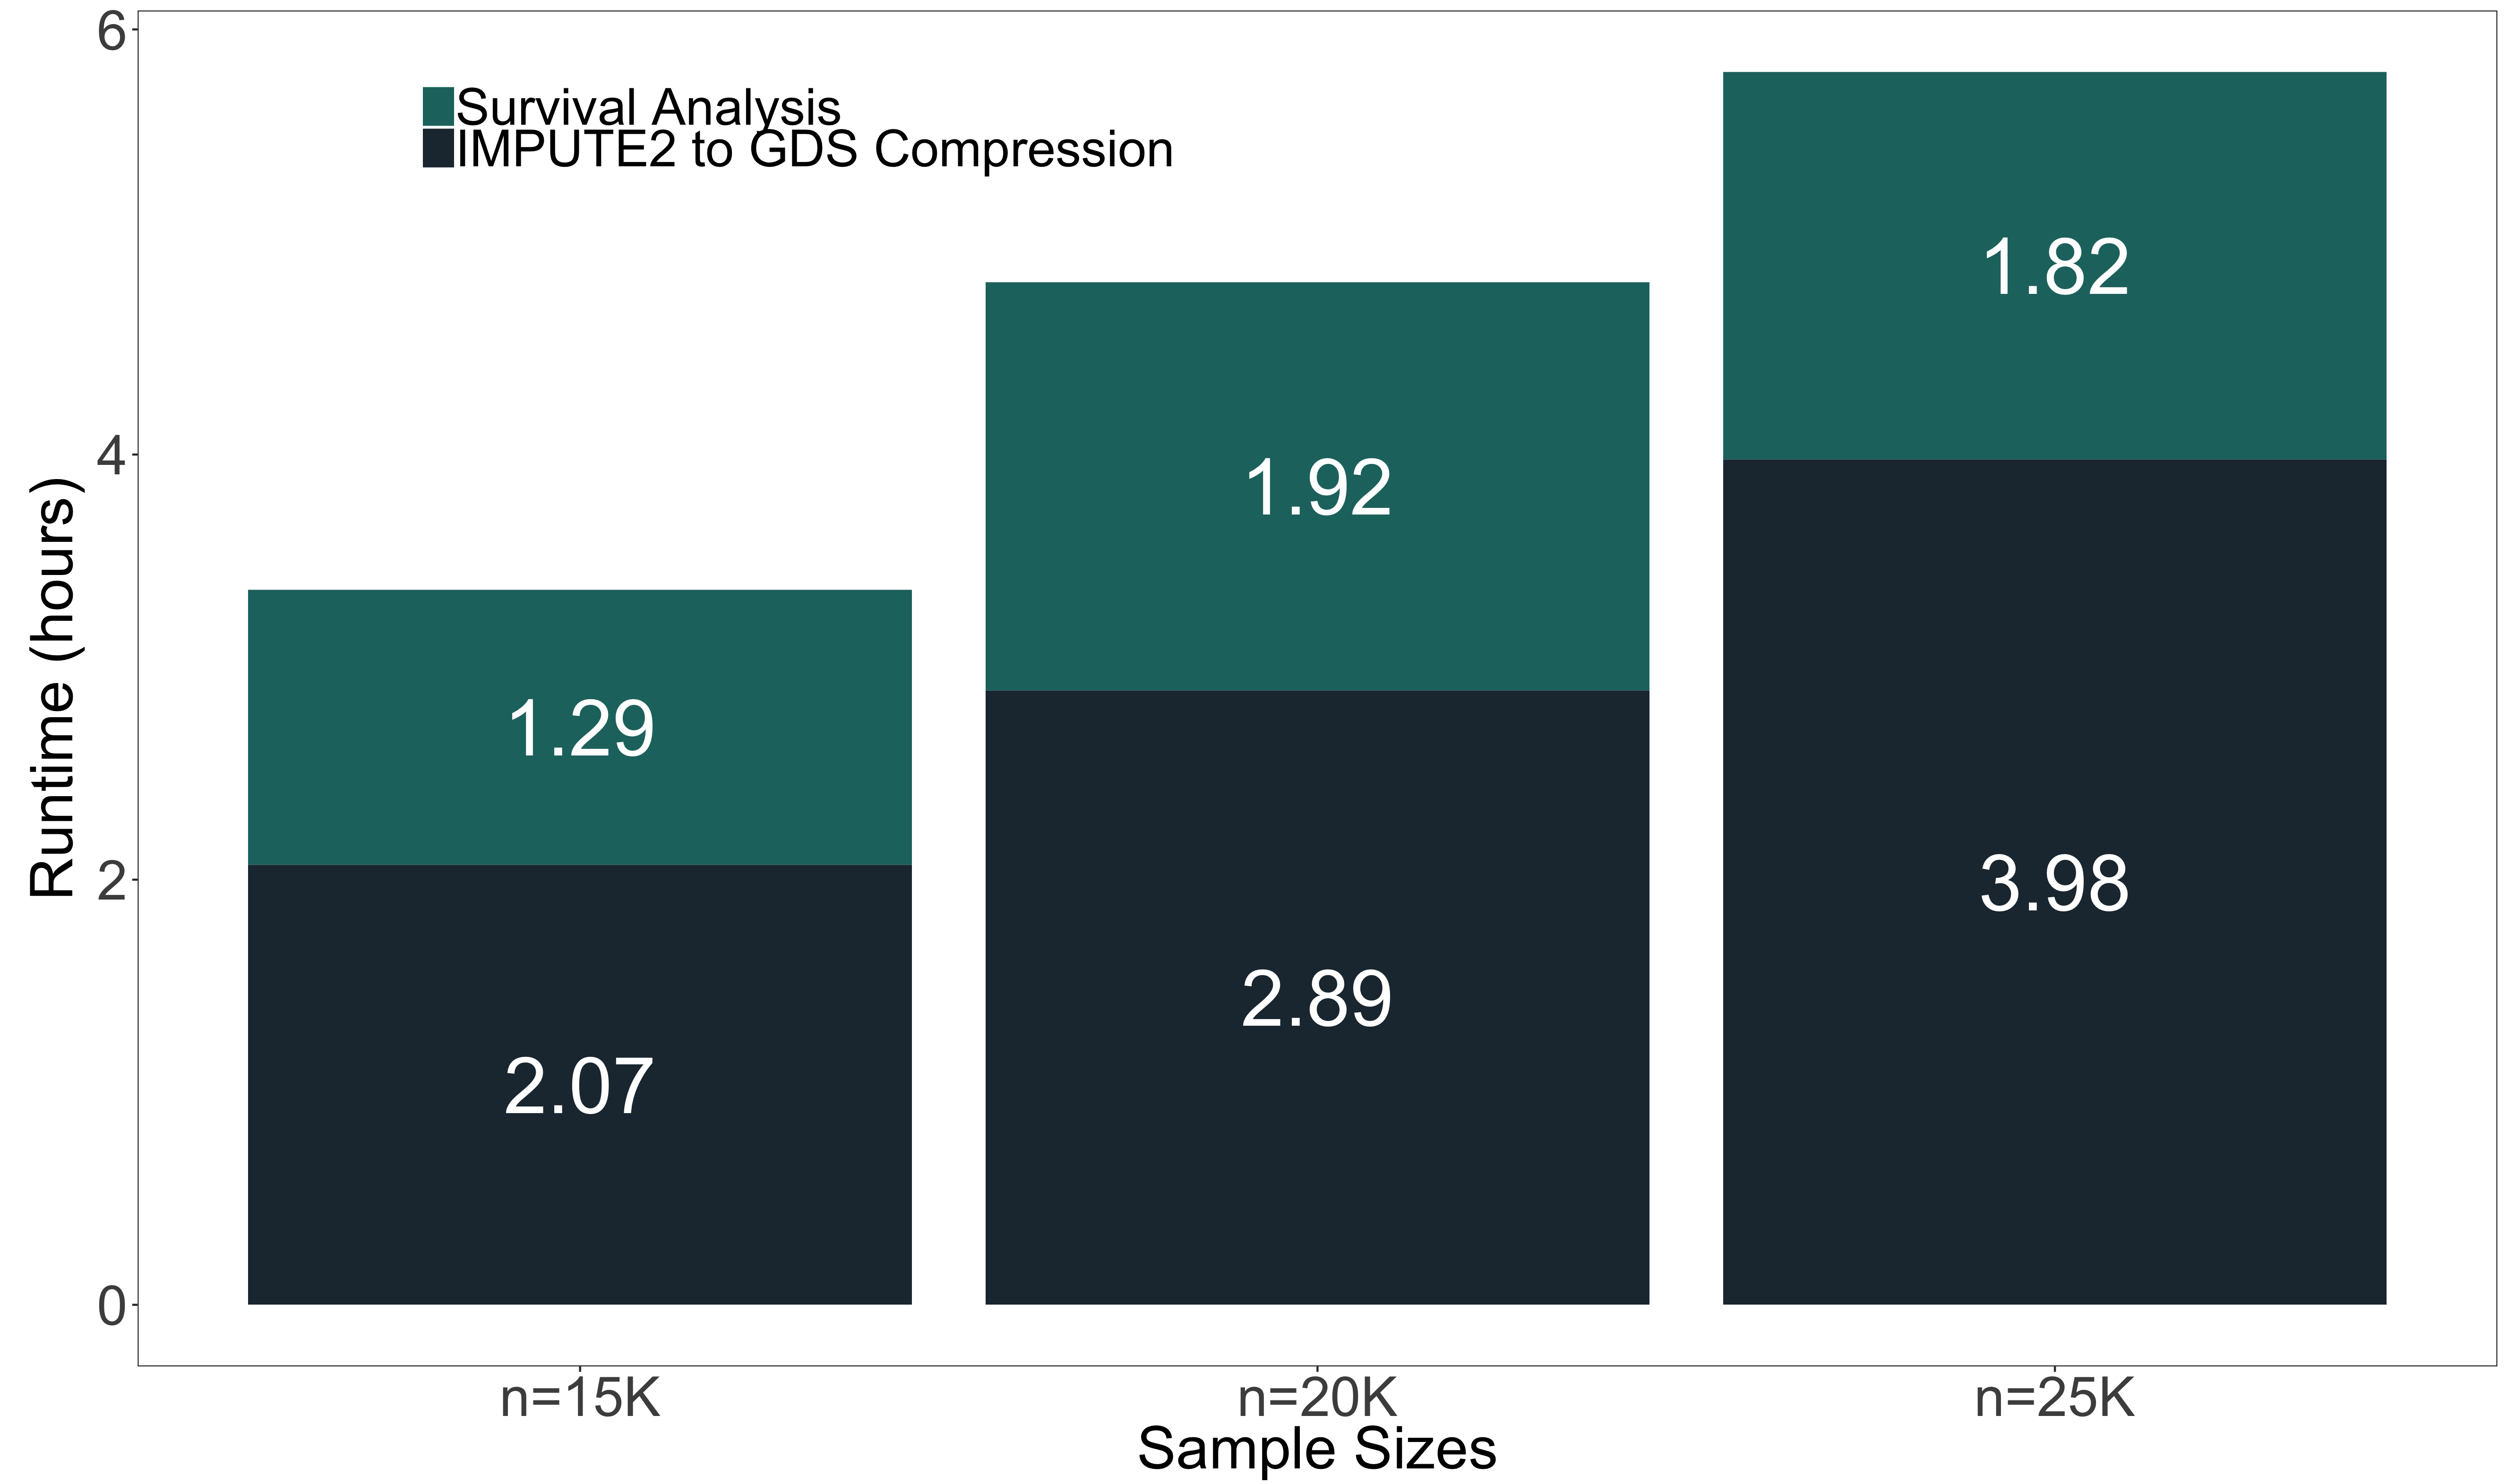
\includegraphics[width=\linewidth, height=3in]{~/Desktop/figures/chapter3/bigN_plot.png}
    \caption[Runtimes for survival analyses with on chromosome 22 with increasing sample size.]{Runtimes for survival analyses with on chromosome 22 with increasing sample size. Gwasurvivr was run on IMPUTE2 data simulated from chromosome 22 ($m \approx 117,000$ SNPs) for $n=15,000$, $n=20,000$ and $n=25,000$. The dark blue is elapsed time for compressing to GDS format and dark green is the computational time to run the survival analysis alone.}
    \label{fig:gwsfig2}  
\end{figure}

As a single GWAS may include tens of thousands of individuals, the next
question was to what extent could the sample size be increased. We
tested \texttt{gwasurvivr} on the smallest chromosome (chromosome 2)
available in our simulated dataset. \texttt{Gwasurvivr} is able to
handle large sample sizes up to \(n=25,000\), however, compression time
increases with increasing sample size, and likely will be limited by
available RAM on a machine or cluster (Figure \ref{fig:gwsfig2}).

\subsubsection{Additional Covariate Runtime: gwasurvivr vs.~other
software}\label{additional-covariate-runtime-gwasurvivr-vs.other-software}

\begin{figure}
    \centering
    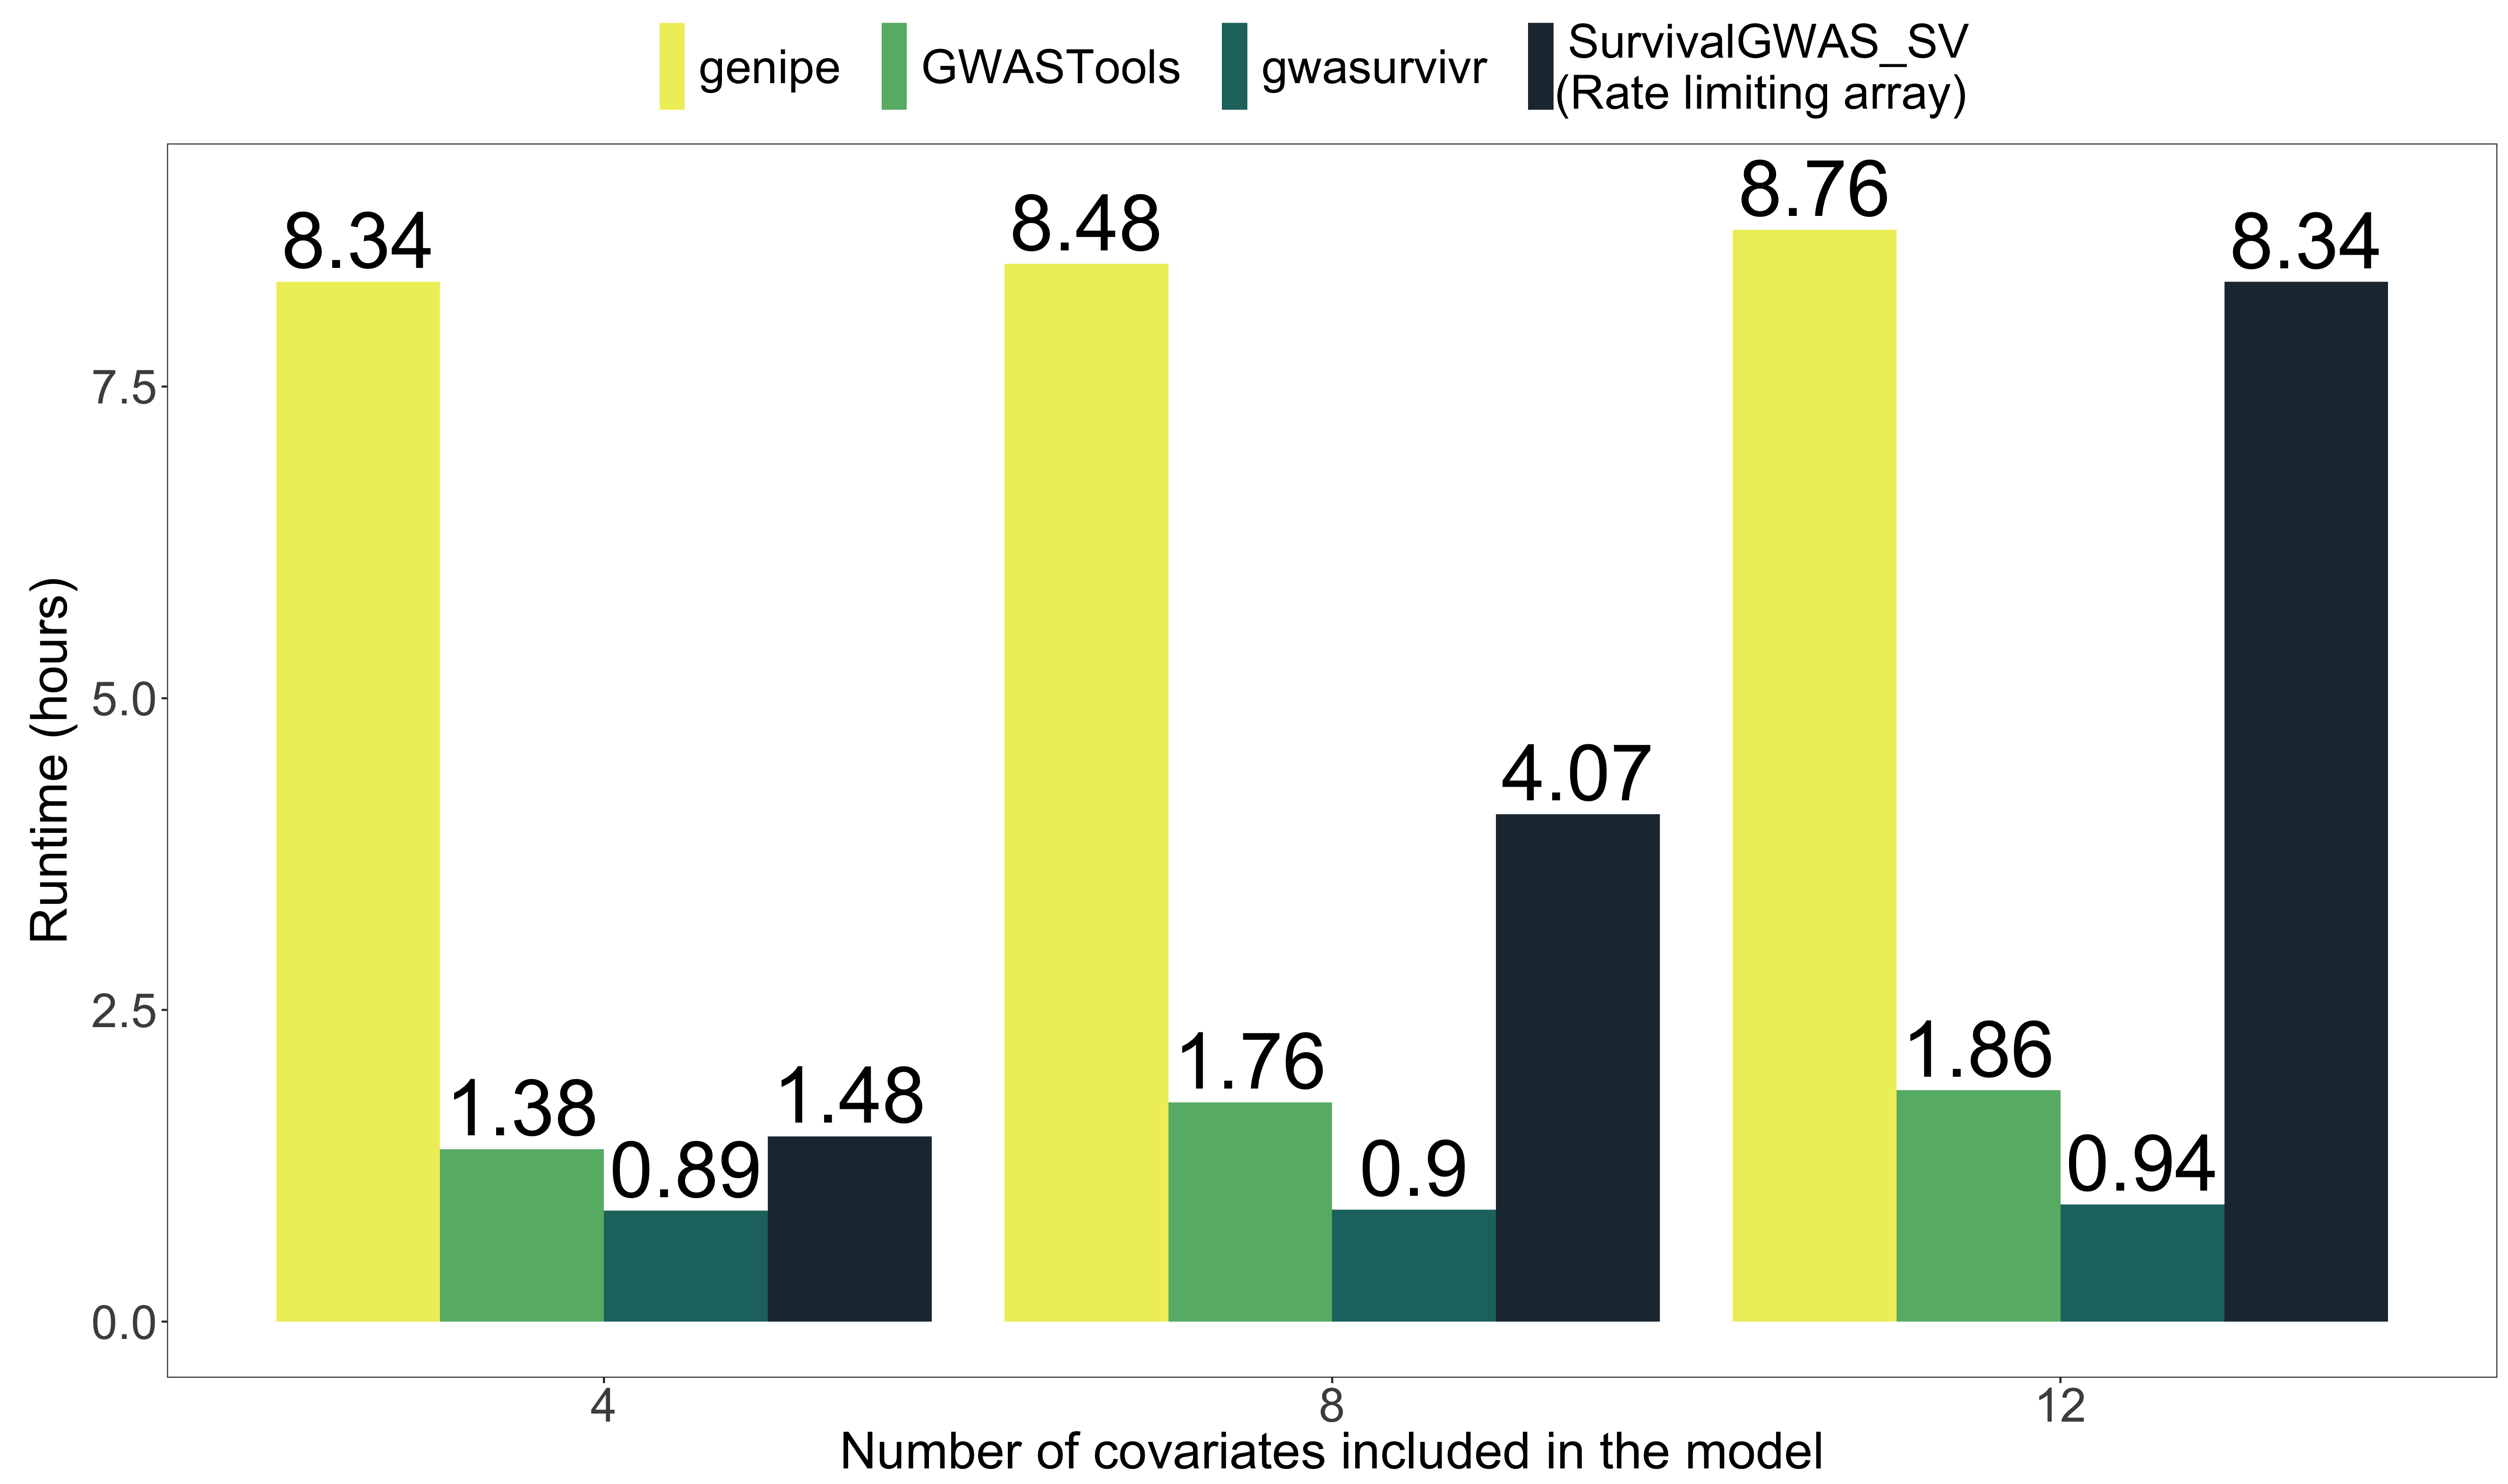
\includegraphics[width=\linewidth, height=3in]{~/Desktop/figures/chapter3/cov_plot.png}
    \caption[Runtime for survival analyses with increasing number of covariates.]{Runtime for survival analyses with increasing number of covariates. Genipe (yellow), GWASTools (light green), SurvivalGWAS\_SV (dark blue) and gwasurvivr (dark green) run with 4, 8 and 12 covariates ($n = 5000$, $m=100,000$).}  
    \label{fig:gwsfig3}  
\end{figure}

We were then interested in how well each software scaled as the number
of additional covariates increased and if a substantial increase in
runtime would occur. Increasing the number of covariates for gwasurvivr
has minimal effects on runtime versus other software (Figure
\ref{fig:gwsfig3}).

\subsubsection{Running full GWAS with different sample sizes using
gwasurvivr}\label{running-full-gwas-with-different-sample-sizes-using-gwasurvivr}

\begin{figure}
    \centering
    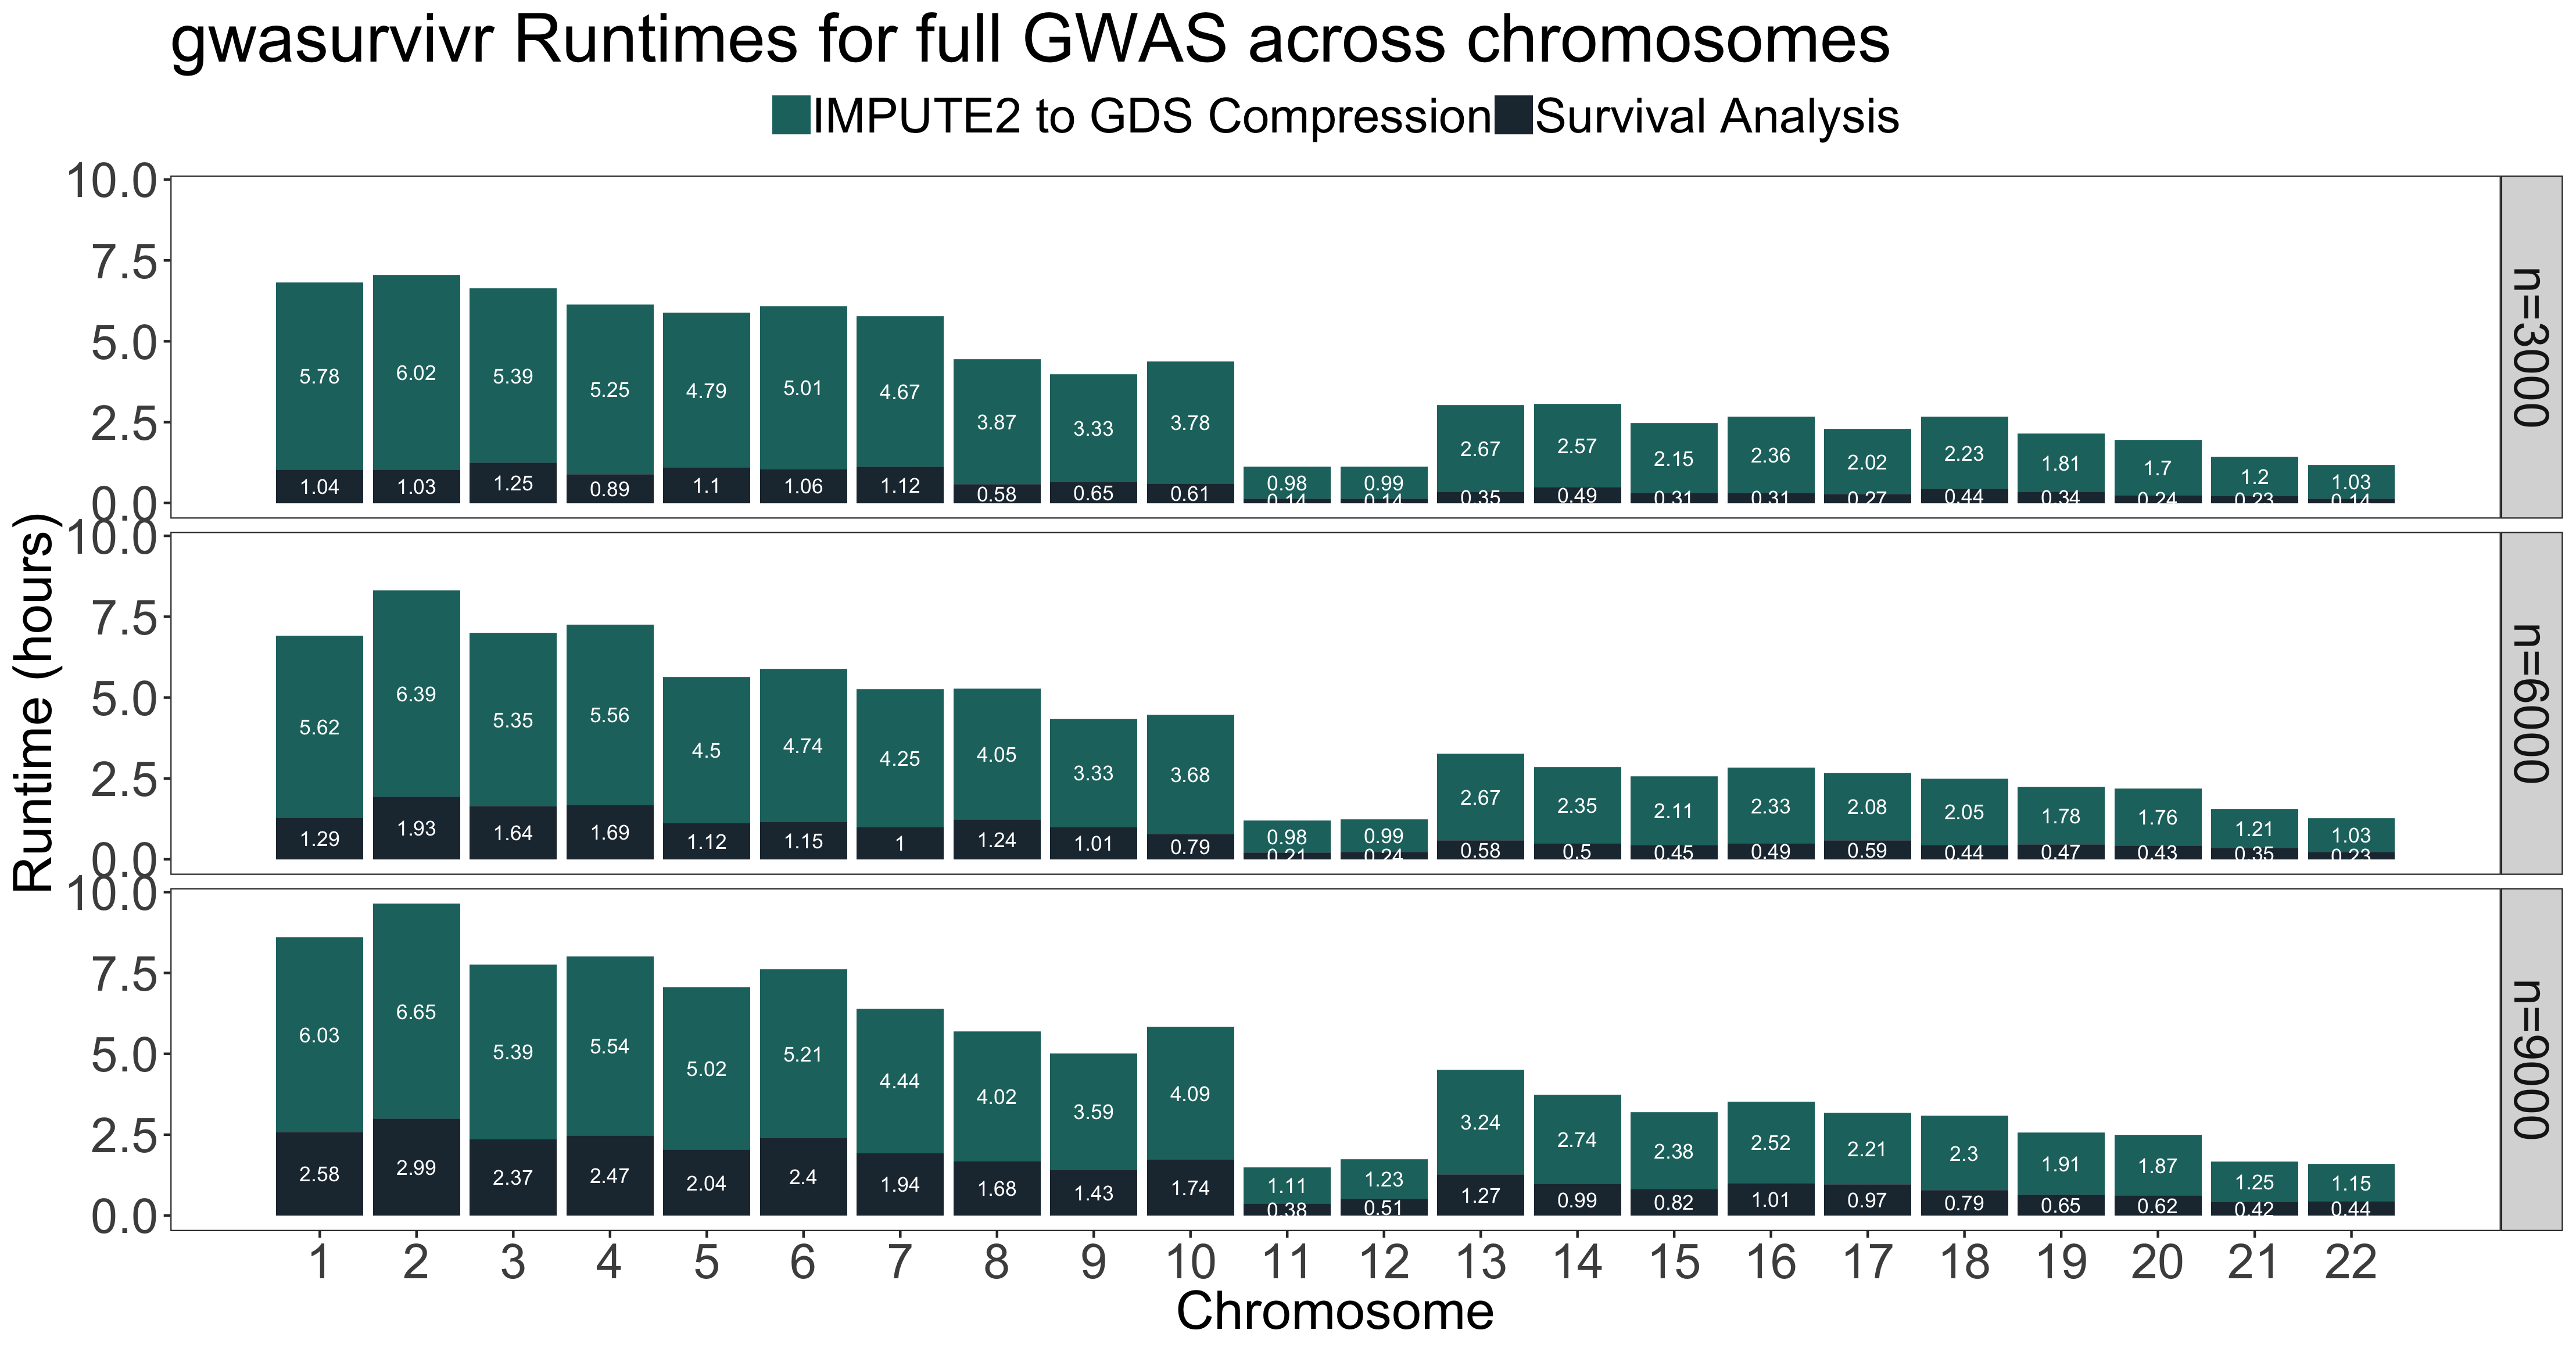
\includegraphics[width=\linewidth, height=6in]{~/Desktop/figures/chapter3/fullgwas_allchrs.png}
    \caption[Runtime for survival analyses for full GWAS with increasing sample size. ]{Runtime for survival analyses for full GWAS with increasing sample size using gwasurvivr impute2CoxSurv. The three panels represent different sample sizes of $n=3000$ (top), $n=6000$ (middle) and $n=9000$ (bottom). The dark blue shaded area is elapsed time for compressing IMPUTE2 to GDS format and the dark green shaded areas are the computational time to run the survival analysis alone. On a computing cluster, each chromosome can be scheduled to run as individual jobs for best performance. Each GWAS was run on the UB CCR supercomputer with on the same node with 24 GB of RAM and 4 CPUs per node.}
    \label{fig:gwsfig4}  
\end{figure}

And the final and most practical question to answer was to determine the
run time for a complete GWAS. A \textasciitilde{}6 million SNP GWAS can
be run in \textless{} 10 hours for 9000 samples when using separately
scheduled jobs on a supercomputer (Figure \ref{fig:gwsfig4}). The
\texttt{keepGDS} argument helps address this and results in reduced run
times (Figures \ref{fig:gwsfig2} and \ref{fig:gwsfig4}), i.e.
\textless{} 3 hours for a GWAS of \(n=9,000\).

\section{Discussion}\label{discussion-2}

Large-scale GWAS that study phenotypes that result in death are becoming
prevalent, particularly in the field of pharmacogenomics. Research
should not be disrupted due to lack of workflows and software that
permit error-free. To put this in persepective, we ran hundreds of
survival analyses in our lab on GWAS data. Often, we would need to
double check analyses before presenting findings at a conference or in a
publication. We lacked reliable software that would enable
straightforward reproducibility, and assumed other labs were
experiencing this as well. A strategy to improve analyses would to
convert all genetic data into GDS and then for subsequent analyses the
survival analyses would complete in a fraction of the time. We could
improve this package by adding visualizations and also by leveraging
SeqVarTools, a new R/Bioconductor package that uses GDS format and
implements row wise computations. An additional useful feature would be
expanding the parallel functionality to compute across nodes rather than
within a single node. We would leverage \texttt{BiocParallel} to
implement this feature. While other software already existed with the
intent of addressing these needs, we developed \texttt{gwasurvivr} be in
the R/Bioconductor ecosystem and be flexible such that it can be easily
integrated into workflows and pipelines, as well as being easily
adjusted for advanced users.

\FloatBarrier

\newpage

\pagestyle{plain} \fancyhead[L]{} \fancyhead[R]{}
\fancyfoot[C]{\thepage} \chapter{Application and Pipeline}
\doublespacing

\section{Introduction}\label{introduction-3}

Automation of large scale studies is essential to the reproducibility of
analyses. Robust workflows that have minimal user interaction decrease
the possibility of continual, unnoticed errors from propagating. When
modeling and analyzing DISCOVeRY-BMT, we often have to compute hundreds
of analyses, i.e.~for three genomes (donor, recipient and mismatch),
different disease stratification, two cohorts, and different survival
outcomes. The effects of both cohorts are combined using meta-analyses.
In order to overcome this potentially cumbersome process, we developed
an automated pipeline that uses imputed genotype data from the Sanger
imputation server as input, runs user specified Cox regression models
using gwasurvivr, performs a meta-analysis, and subsequently reshapes
the data into a clean format. Here we show an overview of the pipeline
(known as DISCOVeRY-BMT Meta-analysis Pipeline) we created and the
analyses that were performed after re-imputing DISCOVeRY-BMT using the
Sanger Imputation Server and describe the functional annotation that
succeeding the initial GWAS.

\section{Methodology}\label{methodology}

\begin{figure}
    \centering
    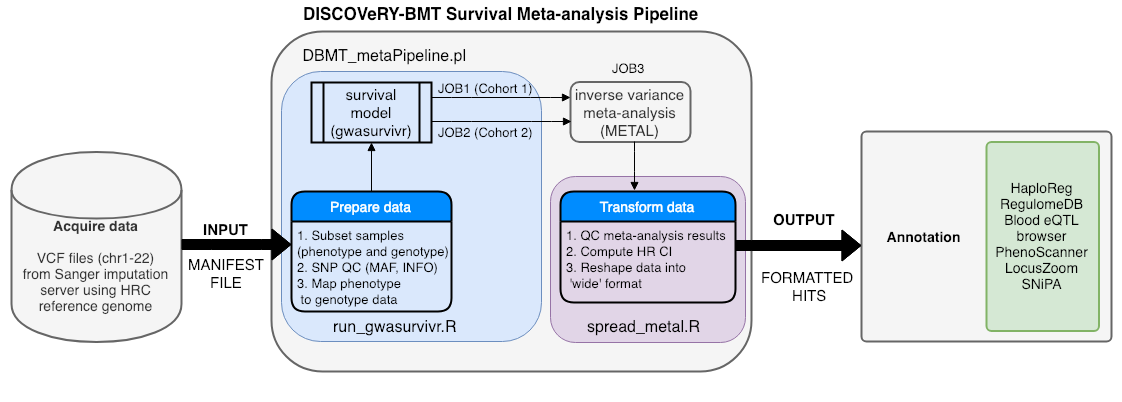
\includegraphics[width=\linewidth, height=3in]{~/Desktop/figures/chapter4/chapter4_flowdiagram_v2.png}
    \caption[Process diagram of automated survival meta-analysis pipeline.]{Process diagram of automated survival meta-analysis pipeline DISCOVeRY-BMT. The pipeline is written in $\texttt{DBMT\_metaPipeline.pl}$. It submits three jobs on UB CCR SLURM, job 1 (cohort 1 survival analysis), job 2 (cohort 2 survival analysis), and job3 (meta-analysis) which waits for (dependency) job 1 and 2 to complete before starting. To elaborate, a manifest file passed to $\texttt{DBMT\_metaPipeline.pl}$ as input that defines the VCF file (chromosome), outcome, patient subset, and memory allocation. $\texttt{run\_gwasurvivr.R}$ captures the command line Rscript that is invoked in the perl script and prepares the data. $\texttt{run\_gwasurvivr.R}$ uses the outcome and patient subset from the manifest file and defines these outcomes and affiliated covariates and runs gwasurvivr survival analysis. After both cohort 1 and cohort 2 are complete, meta-analysis is performed. After meta-analysis is complete, $\texttt{spread\_metal.R}$, filters out heterogeneous SNPs between cohorts, statistics are computed, and data is reformatted such that cohort 1, cohort 2, and meta-analysis are all shown in a single line corresponding to a single variant. The output it then used for annotation to further characterize associations.}
    \label{fig:flow}  
\end{figure}

\rowcolors{2}{gray!6}{white}

\begin{table}[t]

\caption{\label{tab:unnamed-chunk-28}\label{tab:clin_char} Broad Overview of DISCOVeRY-BMT Clinical Characteristics}
\centering
\fontsize{9}{11}\selectfont
\begin{tabular}{c>{\centering\arraybackslash}p{24em}}
\hiderowcolors
\toprule
Genome & Description\\
\midrule
\showrowcolors
Donor & age, sex, race group, blood type (ABO)\\
Recipient & age, sex, race group, blood type (ABO), graft source, causes of death (levels 1-7), conditioning regimen and intensity, TBI fractionation, GVHD prophylaxis, current disease type, current disease progression, prior disease type, cytogenetics status, time to death, time to relapse, AML type, transplant year, HLA match (8/8 or 10/10), cytomegalyvirus, Lansky Score, Karnovsky Score, Principal Components from EIGENSTRAT\\
\bottomrule
\end{tabular}
\end{table}

\rowcolors{2}{white}{white}

\subsection{Data}\label{data}

\subsubsection{Genetic Data (Imputation
Results)}\label{genetic-data-imputation-results}

DISCOVeRY-BMT was first imputed using IMPUTE2 (B. N. Howie, Donnelly,
and Marchini \protect\hyperlink{ref-Howie_2009}{2009}) and 1000 Genomes
Project (1kGP) Phase 3 (1000 Genomes Project Consortium
\protect\hyperlink{ref-1000genomes}{2015}) reference panel. Although new
reference panels have not updated to a newer genome release than Genome
Reference Consortium Human Build 37 (GRCh37; same as 1kGP), the number
of samples included in the development of the reference panel itself
have increased substantially (i.e.~from \(\approx 1000\) to
\(\approx 65,000\). As such we decided that it would be appropriate to
update DISCOVeRY-BMT GWAS data to increase the quality of imputation.

As mentioned in Chapter 1 and Chapter 3, several imputation software and
servers exist. Two imputation web services are publicly available,
Michigan imputation server (Das et al.
\protect\hyperlink{ref-michigan_imputation}{2016}) from University of
Michigan and Sanger imputation server from Wellcome Sanger Institute
(McCarthy et al. \protect\hyperlink{ref-hrc}{2016}). The largest,
non-subtle, differences between the servers are related to the
imputation algorithms used. Michigan imputation server uses minimac3
(Das et al. \protect\hyperlink{ref-michigan_imputation}{2016}). Sanger
imputation server using the position Burrows-Wheeler transform (PBWT)
algorithm (R. Durbin \protect\hyperlink{ref-durbin_2014}{2014}). Both
imputation services offer user friendly platforms and offer the most up
to date reference panels, including HRC release 1.1. HRC reference panel
combines data from over 20 different studies. The majority of samples in
HRC are low coverage sequencing data and predominantly European
ancestry, and HRC includes 1kGP Phase 3 as well. HRC has
\(\approx 65,000\) haplotypes and \(\approx 40\) million SNPs. Prior to
imputation, it is common practice it is common practice to pre-phase
(haplotype estimation) before imputation, as previous studies have
demonstrated estimating haplotypes prior to imputation substantially
speeds up the imputation process (O'Connell et al.
\protect\hyperlink{ref-OConnell_2016}{2016}). EAGLE2 (P.-R. Loh et al.
\protect\hyperlink{ref-eagle2}{2016}) or SHAPEIT2 (Delaneau et al.
\protect\hyperlink{ref-shapeit2}{2013}) are commonly used pre-phasing
algorithms. SHAPEIT2 pre-phasing and PBWT imputation were used for
DISCOVeRY-BMT, returning unphased, imputed genotypes.

\subsubsection{Phenotype file}\label{phenotype-file}

DISCOVeRY-BMT has clinical characteristics and survival times/events
corresponding to recipients and donors provided by NMDP and CIBMTR. The
phenotype file will interchangeably be referred to as ``covariate
file''. The survival times and events are for recipients only.
Characteristics are shown in Table \ref{tab:clin_char}. In the phenotype
file that is used for our analyses -- many clinical covariates been
recoded into dummy/indicator variables or stratified into joint
groupings.

\subsection{Perl Script for Pipeline}\label{perl-script-for-pipeline}

The perl script resides on UB CCR and is very specific to DISCOVeRY-BMT
and folder structure on our accounts. The central idea is that the
pipeline consists of three jobs (JOB1, JOB2, and JOB3) in a single Slurm
Workload Manager submission. JOB1 and JOB2 are perform survival analysis
using gwasurvivr on VCF files for one chromosome (Figure
\ref{fig:flow}). JOB3 is the meta-analysis of cohorts 1 and 2 using
METAL (Willer, Li, and Abecasis \protect\hyperlink{ref-metal}{2010})
software. JOB3 also reshapes the data such that results from cohort 1,
cohort 2, and meta-analysis are all in one row. JOB3 has a dependency on
JOB1 and JOB2 completion before initiating (Figure \ref{fig:flow}).

\subsubsection{Manifest file}\label{manifest-file}

The imputed files can be directly passed to gwasurvivr. Manifest files
are defined as a file that contains columns (for this pipeline, manifest
files are tab-separated) that describe specific arguments that are
passed to other functions (i.e. \texttt{run\_gwasurvivr.R} or SLURM
scripts). Manifest file fields can be found in Table 2.

\rowcolors{2}{gray!6}{white}

\begin{table}[t]

\caption{\label{tab:unnamed-chunk-29}Manifest file column descriptions}
\centering
\fontsize{9}{11}\selectfont
\begin{tabular}{c>{\centering\arraybackslash}p{36em}}
\hiderowcolors
\toprule
Column name & Description\\
\midrule
\showrowcolors
path\_to\_vcf\_file & Chromosomes 1-22 VCF files (include full directory)\\
output\_name & Output file name\\
patient\_subset & Patient subset - i.e. ALL only, AML only, Mixed\\
genome & Donor, recipient, or mismatch\\
outcome & Outcome - i.e. DRM, TRM, OS, PFS, INF, OF, REL\\
\addlinespace
memory & Random access memory (RAM) in megabytes (MB) allocated to the job\\
\bottomrule
\end{tabular}
\end{table}

\rowcolors{2}{white}{white}

\subsubsection{Execution of script}\label{execution-of-script}

\rowcolors{2}{gray!6}{white}

\begin{table}[t]

\caption{\label{tab:unnamed-chunk-30}\label{tab:jobs_run} DISCOVeRY-BMT Analyses Run Using DBMT metaPipeline.}
\centering
\fontsize{9}{11}\selectfont
\begin{tabular}{>{\raggedright\arraybackslash}p{6em}>{\raggedright\arraybackslash}p{4em}>{\raggedright\arraybackslash}p{8em}>{\raggedright\arraybackslash}p{6em}>{\raggedright\arraybackslash}p{4em}}
\hiderowcolors
\toprule
Genomes & Patient Subset & Survival Outcomes & Censoring Time & Analyses Run\\
\midrule
\showrowcolors
Donor, Recipient, Mismatch & AML & DRM, TRM, OS, PFS & 1 year & 12\\
Donor, Recipient, Mismatch & AML + MDS & DRM, TRM, OS, PFS & 1 year & 12\\
Donor, Recipient, Mismatch & Mixed & DRM, TRM, OS, PFS & 1 year & 12\\
Donor, Recipient & ALL & DRM, TRM, OS, PFS, REL, OF, GVHD, INF & 1 year & 16\\
Donor, Recipient & B-ALL & DRM, TRM, OS, PFS & 1 year & 8\\
\addlinespace
Donor, Recipient & T-ALL & DRM, TRM, OS, PFS & 1 year & 8\\
Donor, Recipient, Mismatch & ALL & DRM, TRM, OS, PFS, REL, INF, OF, GVHD & 100 days & 24\\
Donor, Recipient, Mismatch & AML & DRM, TRM, OS, PFS, REL, INF, OF, GVHD & 100 days & 24\\
Donor, Recipient, Mismatch & AML + MDS & DRM, TRM, OS, PFS, REL, INF, OF, GVHD & 100 days & 24\\
Donor, Recipient, Mismatch & Mixed & DRM, TRM, OS, PFS, REL, INF, OF, GVHD & 100 days & 24\\
\addlinespace
Donor, Recipient & ALL & OS, REL & 3 years & 4\\
\hline
Total &  &  &  & 168\\
\bottomrule
\end{tabular}
\end{table}

\rowcolors{2}{white}{white}

Essentially the script facilitates submission of survival analysis for
JOB1, JOB2, and JOB3.

Required commands:

\singlespacing

\begin{verbatim}
    -m        path to the manifest file
    -e        e-mail address for SLURM status updates 
              (completion of run)
    -w        walltime in format 00:00:00
    -rscript  The R script (run_gwasurvivr.R) that internalizes 
              arguments from the manifest file, assigns outcomes 
              and corresponding covariates. And then invokves 
              gwasurvivr for both cohort 1 and cohort 2.
\end{verbatim}

\doublespacing

For example, shown below is the command to execute the pipeline for
recipients with AML when testing for DRM:

\singlespacing

\begin{Shaded}
\begin{Highlighting}[]
\FunctionTok{perl}\NormalTok{ /projects/rpci/lsuchest/lsuchest/DBMT_metaPipeline/\textbackslash{}}
\NormalTok{        Meta_pipeline.pl \textbackslash{}}
\NormalTok{    -m D_AMLonly_DRM.manifest \textbackslash{}}
\NormalTok{    -e rizvi.33@osu.edu \textbackslash{}}
\NormalTok{    -w 08:00:00 \textbackslash{}}
\NormalTok{    -rscript /projects/rpci/lsuchest/lsuchest/DBMT_metaPipeline/\textbackslash{}}
\NormalTok{        run_gwasurvivr.R }
\end{Highlighting}
\end{Shaded}

\doublespacing

\subsection{GWAS Analyses Run}\label{gwas-analyses-run}

\rowcolors{2}{gray!6}{white}

\begin{table}[t]

\caption{\label{tab:unnamed-chunk-32}\label{tab:models_run} Survival Models Analyzed}
\centering
\fontsize{9}{11}\selectfont
\begin{tabular}{lll}
\hiderowcolors
\toprule
Survival Outcomes & Time Interval & Covariates\\
\midrule
\showrowcolors
TRM & time to death & recipient age, BMI, graft source\\
DRM & time to death & recipient age, disease status\\
OS & time to death & age, disease status, graft source\\
PFS & time to relapse & recipient age, disease status\\
REL & time to relapse & conditioning regimen and intensity\\
\addlinespace
GVHD & time to death & recipient age, donor age, BMI\\
OF & time to death & disease status, graft source\\
INF & time to death & age, BMI, CMV status\\
\bottomrule
\end{tabular}
\end{table}

\rowcolors{2}{white}{white}

\begin{figure}
    \centering
    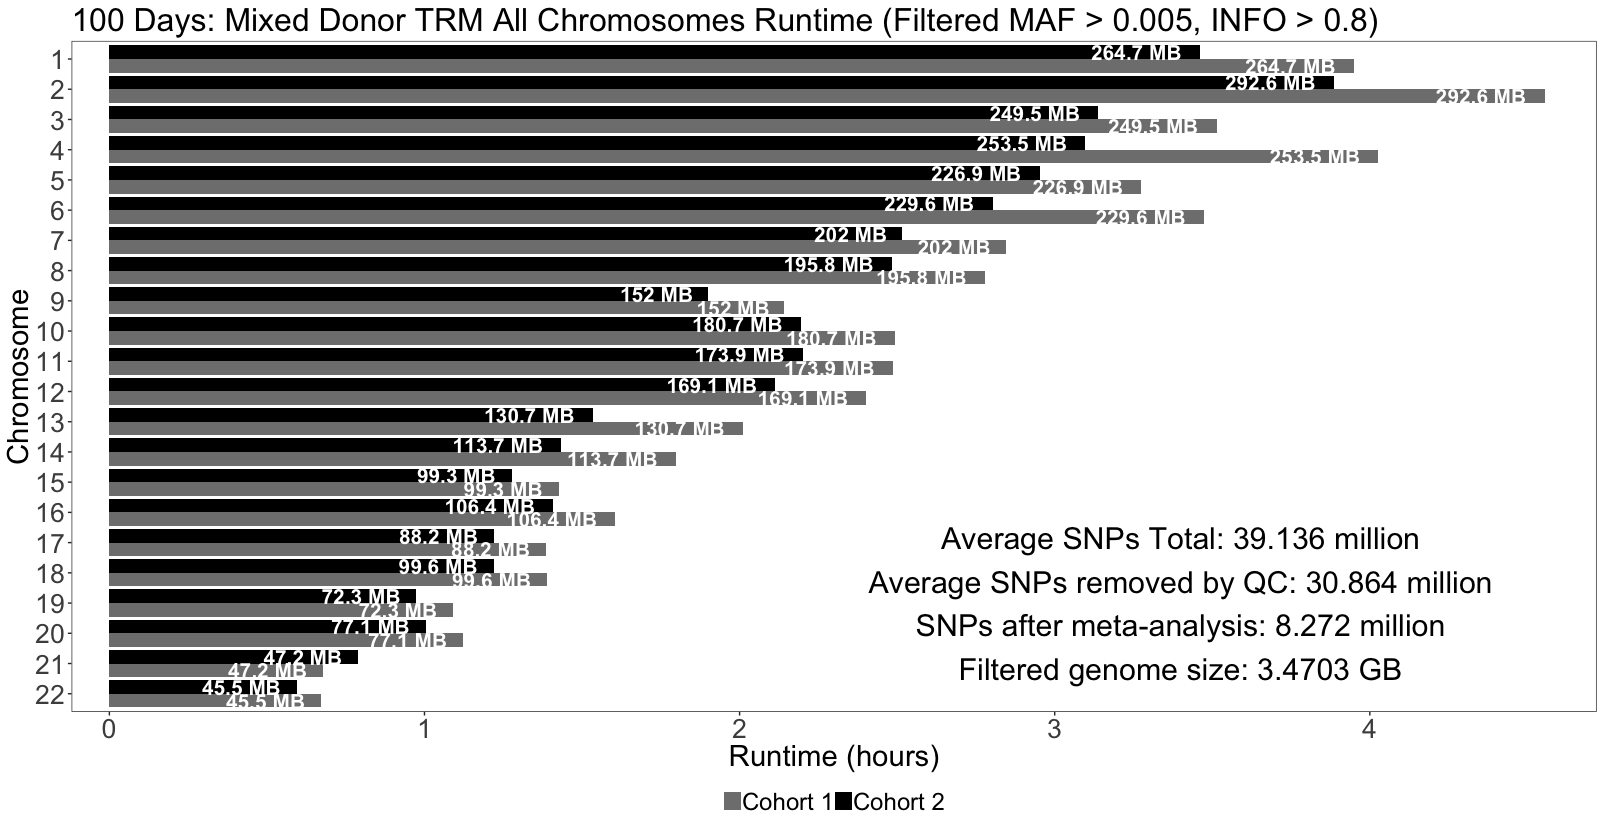
\includegraphics[width=\linewidth, height=5in]{~/Desktop/figures/chapter4/trm_mixed_run_times.png}
    \caption[Runtime diagnostics of full GWAS using DBMT Meta analysis Pipeline.]{Runtime diagnostics of full GWAS using DBMT Meta analysis Pipeline. Shown here is just one example of all analyses run. This example is donor genotypes in mixed diseases (AML + ALL + MDS) recipients, testing for TRM. The y-axis is chromosomes 1-22 and the x-axis is computational runtime in hours. Each chromosome was run separately and all began at the same time, such that the total time for this GWAS was equivalent to chromosome 2 in cohort 1 runtime (4.66 hours). The white text inside each bar is the file size of the chromosomes after gwasurvivr survival analysis. The SNPs were filtered for MAF > 0.005 and INFO > 0.8.}
    \label{fig:run_times}  
\end{figure}

We ran 168 different analyses (504 analysis jobs total) (Table
\ref{tab:jobs_run}). The clinical covariates that we included in our
models are in Table \ref{tab:models_run}. The clinical covariates were
selected as they pertained to clinical relevance. For covariates in REL,
the model was selected using bidirectional stepwise regression. Although
we ran hundreds of analyses, we will only discuss ALL analyses censored
at 1-year in Chapter 5. Each GWAS took just over 4 hours when submitting
entire GWAS at the same time on UB CCR (Figure \ref{fig:run_times}).
Instances of delay of analysis due to backlog in Slurm Workload queue
were rare. An entire genome began at \(\approx 40\) million SNPs and
after QC (INFO \textgreater{} 0.8, MAF \textgreater{} 0.005, filtering
out SNPs that did not converge from Cox model), the final genome was
\(\approx 8\) million SNPs, or the equivalent to 3.47 GB of storage
(Figure \ref{fig:run_times}).

\subsection{Post-GWAS Analyses}\label{post-gwas-analyses}

While GWAS in and of itself is a powerful method to identify
disease-associated SNPs, it does not necessarily address the underlying
biology the association signals. After the meta-analysis GWAS are
complete, we first looked at our association signals. To visualize this,
we created our own custom Manhattan plot in \texttt{ggplot2} (Wickham
\protect\hyperlink{ref-ggplot2}{2016}), that labels the SNPs that are
below \(P_{meta} < 5\times{10}^{-8}\) threshold (code available on
dissertation GitHub repository). The next step was to use publicly
available data resources to annotate SNPs that reached the suggestive
significance threshold \(P_{meta} < 5\times{10}^{-5}\). Annotation aids
researchers develop mechanistic hypotheses to further characterize the
impact of non-coding variants on clinical phenotypes and/or normal
genetic variation. Annotation was done by leveraging publicly available
databases that have compiled data from large scale studies (ENCODE,
GTEx) using HaploReg (L. D. Ward and Kellis
\protect\hyperlink{ref-haploreg}{2015}), RegulomeDB (Boyle et al.
\protect\hyperlink{ref-Boyle_2012}{2012}), and single nucleotide
polymorphisms annotator (SNiPA) (Arnold et al.
\protect\hyperlink{ref-snipa}{2015}).

\subsubsection{Annotation Resources}\label{annotation-resources}

HaploReg leverages LD information from the 1000 Genomes Project to
compile chromatin states and protein binding annotation from ENCODE and
Roadmap to Epigenome projects (L. D. Ward and Kellis
\protect\hyperlink{ref-haploreg}{2015}). HaploReg also collects and
curates data from sequence conservation studies, as well as studies that
determine effects of SNPs and consequences on regulatory motifs and/or
gene expression (eQTL) (L. D. Ward and Kellis
\protect\hyperlink{ref-haploreg}{2015}). HaploReg data was accessed
using haploR (Zhbannikov, Arbeev, and Yashin
\protect\hyperlink{ref-haploR}{2019}).

RegulomeDB is a collection of annotation databases that reports SNPs
with known and/or predicted regulatory elements in intergenic regions of
the human genome (Boyle et al.
\protect\hyperlink{ref-Boyle_2012}{2012}). Known and predicted
regulatory DNA elements include regions of DNAase hypersensitivity,
binding sites of transcription factors (TFs), and promoter regions that
have been experimentally/biochemically characterized to regulate
transcription (Boyle et al. \protect\hyperlink{ref-Boyle_2012}{2012}).
The entire RegulomeDB database was downloaded and stored on UB CCR for
ease of access when annotating regions of interest.

SNiPA annotations come from Ensembl87 (v3.2). It comprises
variant-phenotype associations and annotations contained in Ensembl 92
release, as well as pQTL data. pQTL association data is s obtained from
the pGWAS study in blood (B. B. Sun et al.
\protect\hyperlink{ref-sun_2018}{2018}). SNiPA includes more than 16,500
cis- and trans-associations with blood protein levels (Arnold et al.
\protect\hyperlink{ref-snipa}{2015}). The genome assembly for SNiPA is
GRCh37.p13 and it uses 1000 Genomes Project Phase 3 (v5). SNiPA obtains
data from HGMD, dbGaP, ClinVar, OMIM variation, UniProt, GWAS Catalog,
DrugBank, DECIPHER, and GTEx eQTL associations (Arnold et al.
\protect\hyperlink{ref-snipa}{2015}). Flanking regions of +/- 150kb from
the sentinel SNP (snp of interest) are pulled from DISCOVeRY-BMT
results.

The R code and SLURM scripts for data manipulating and pulling regions
for HaploReg, RegulomeDB, and SNiPA are available on this dissertation's
GitHub repostiory.

\section{Discussion}\label{discussion-3}

In this chapter we described the fulcrum to all of analyses run in
DISCOVeRY-BMT Sanger imputation results. We developed a pipeline that
facilitated automation of hundreds of survival analyses that ensured
ease of implementation and reproducibility. We also described post-GWAS
analyses that have yet to be integrated into this pipeline. An ongoing
project is underway that will unite an annotation (SNiPA, HaploReg, and
RegulomeDB) workflow with our current pipeline. As the phenotype of
DISCOVeRY-BMT is quite complex, this will allow our lab to uncover
insights in a much more reproducible and less cumbersome manner.
Additional databases such as PhenoScanner (Staley et al.
\protect\hyperlink{ref-staley_2016}{2016}) and Blood eQTL Browser
(Westra et al. \protect\hyperlink{ref-westra_2013}{2013}) will also be
implemented into the annotation portion of this pipeline.

\FloatBarrier

\newpage

\pagestyle{plain} \fancyhead[L]{} \fancyhead[R]{}
\fancyfoot[C]{\thepage}

\chapter{Death within 1 year after MUD-HSCT for Acute Lymphoblastic Leukemia (ALL) GWAS}

\doublespacing

\section{Introduction}\label{introduction-4}

Acute lymphoblastic leukemia (ALL) is a type liquid cancer that
originates in the lymphoid line of hematopoietic stem cells. It the most
common type of childhood cancer (25\% of all cases) and about 60\% of
cases for those under 20 years old worldwide (Pui
\protect\hyperlink{ref-pui2011acute}{2011}). Childhood ALL is highly
treatable with a combination of standard chemotherapy protocols with a
5-year survival is upwards of 90\% (Pui et al.
\protect\hyperlink{ref-pui_2015}{2015}). Historically adolescents and
young adults (AYA) have had poorer prognosis when it came to treatment
from ALL, however, over the past several years major improvements have
occurred as treatment protocols have shifted from treating AYA with
adult regimens towards pediatric regimens (Huguet et al.
\protect\hyperlink{ref-Huguet_2009}{2009}; Siegel et al.
\protect\hyperlink{ref-siegel_2018}{2018}).

While therapeutic regimens have been quite successful, ALL remains the
second most common hematological malignancy for which patients will
undergo HLA-matched unrelated donor hematopoietic stem cell
transplantation (MUD-HSCT) (D'Souza et al.
\protect\hyperlink{ref-DSouza_2017}{2017}). The number of transplants
among ALL patients has steadily been increasing yearly (D'Souza et al.
\protect\hyperlink{ref-DSouza_2017}{2017}). As recently as 2017, there
was approximately 6,000 new cases of ALL and approximately 1500 patients
underwent MUD-HSCT (SEER Database \protect\hyperlink{ref-seer}{2018};
D'Souza et al. \protect\hyperlink{ref-DSouza_2017}{2017}). ALL patients
receive HSCT as a curative therapy after reaching complete remission
(CR) and disease status at time of diagnosis play a major role in
disease prognosis (Pui \protect\hyperlink{ref-pui2011acute}{2011}).
Patients receive HSCT as a curative therapy after reaching complete
remission (CR) and disease status at time of diagnosis play a major role
in disease prognosis. Nearly 60\% of adult (\(\geq 40\) years old)
patients with advanced disease die within the first year after
transplant (D'Souza et al. \protect\hyperlink{ref-DSouza_2017}{2017}).
MUD-HSCT has slightly improved survival in childhood ALL (\(\leq 15\)
years old) with 40\% of advanced disease patients dying in the first
year (D'Souza et al. \protect\hyperlink{ref-DSouza_2017}{2017}). These
large proportions of patients dying within the first year present a
strong need to discover genetic markers that can inform clinicians on
patient longevity and/improvements in donor selection.

Here, we use DISCOVeRY-BMT GWAS to identify and characterize germline
genetic markers contribution to survival in ALL patients and their
matched unrelated donor after MUD-HSCT. While this study is not
specifically asking questions about age, over 60\% the ALL patient
population in DISCOVeRY-BMT are in childhood and AYA populations,
presenting an excellent cohort to uncover markers that may contribute to
poor outcomes in young and adult patients after transplant.
Additionally, targeted therapeutics can be discovered from SNPs,
particularly those that alter sequences of transcription factor binding
or result in epigenetic remodeling. In this chapter we go through
associated regions for recipient survival outcomes when considering
either recipient or their unrelated donor genetics. Furthermore, we
performed post-GWAS annotation to develop mechanistic and biologically
relevant hypotheses of how these SNPs contribute to survival phenotypes.

\section{Methods}\label{methods-2}

Chapter 1 provides details on DISCOVeRY BMT cohorts and survival outcome
definitions. Chapter 4 describes the clinical covariates included in all
analyses and provides an in depth description of analytic methods. Acute
lymphoblastic leukemia patients in DISCOVeRY-BMT are cytogenetically
normal. We use Cox regression (Cox
\protect\hyperlink{ref-cox1972}{1972}; A. A. Rizvi et al.
\protect\hyperlink{ref-Rizvi_2018}{2018}) to test the significance of
genetic variation in: overall survival (OS), disease related mortality
(DRM), transplant related mortality (TRM), relapse (REL),
progression-free survival (PFS) and TRM subtypes {[}graft versus host
disease (GVHD), infection (INF), and organ failure (OF){]}.

All analyses were performed on one SNP (donors or recipients dosage
across all patients) at a time, adjusted for clinically relevant
covariates. Meta-analysis was done using a fixed effects model via METAL
software (Willer, Li, and Abecasis \protect\hyperlink{ref-metal}{2010}).
Additional QC was performed on the SNPs (i.e.~INFO score \textgreater{}
0.8, MAF \textgreater{} 0.05 in both cohorts, required to be same
direction between cohorts and heterogeneous SNPs were filtered out). We
define genome-wide significance as \(P_{meta} < 5 \times{10}^{-8}\).
Reported significant results were filtered
\(P_{\text{cohort1}} < 5\times{10}^{-5}\) and
\(P_{\text{cohort2}} < 0.2\). Meta-hazard ratios were filtered
\(\frac{1}{15} \leq \text{HR}_{meta} \leq 15\).

Post-GWAS annotations were performed by leveraging publicly available
databases including HaploReg v4.1 (L. D. Ward and Kellis
\protect\hyperlink{ref-haploreg}{2015}), RegulomeDB (Boyle et al.
\protect\hyperlink{ref-Boyle_2012}{2012}), and SNiPA (Arnold et al.
\protect\hyperlink{ref-snipa}{2015}). These annotation repositories were
described in detail in Chapter 4.

\section{Results}\label{results-2}

\subsection{DISCOVeRY-BMT ALL Summary}\label{discovery-bmt-all-summary}

\rowcolors{2}{gray!6}{white}

\begin{table}[t]

\caption{\label{tab:unnamed-chunk-33}\label{tab:all_event_props} Proportion of Events at 1-year in DISCOVeRY-BMT ALL Cohorts}
\centering
\fontsize{9}{11}\selectfont
\begin{threeparttable}
\begin{tabular}{ccc}
\hiderowcolors
\toprule
Outcome & Cohort 1 & Cohort 2\\
\midrule
\showrowcolors
DRM & 91/483 (0.188) & 19/94 (0.202)\\
TRM & 108/483 (0.224) & 20/94 (0.213)\\
OS & 199/483 (0.412) & 39/94 (0.415)\\
PFS & 245/483 (0.507) & 45/94 (0.479)\\
REL & 133/483 (0.275) & 25/94 (0.266)\\
\addlinespace
GVHD & 37/483 (0.077) & 4/94 (0.043)\\
INF & 32/483 (0.066) & 9/94 (0.096)\\
OF & 28/483 (0.058) & 5/94 (0.053)\\
\bottomrule
\end{tabular}
\begin{tablenotes}[para]
\item Proportion of Events (Death or Relapse) are displayed as the sample size of event ($\text{N}_{\text{event}}$) divided by the total number of patients (N) in the ALL cohort. Overlapping events are not shown here.
\end{tablenotes}
\end{threeparttable}
\end{table}

\rowcolors{2}{white}{white}

DISCOVeRY-BMT has 483 patients in cohort 1 and 94 patients in cohort 2
(Table \ref{tab:all_event_props}). The proportion of patients that die
within the first year (overall survival) is on average 41.35\% between
both cohorts (Table \ref{tab:all_event_props}). Slightly more patients
die from TRM than from DRM at 21.85\% and 19.5\% between both cohorts,
respectively (Table \ref{tab:all_event_props}). About 27\% of patients
experience relapse after transplant and between 5-7\% of patients are
dying from TRM subtypes (Table \ref{tab:all_event_props}).

\rowcolors{2}{gray!6}{white}

\begin{table}[t]

\caption{\label{tab:unnamed-chunk-34}\label{tab:all_ages} Proportion of ALL Patient Age Groups Stratified by DISCOVeRY-BMT Cohorts}
\centering
\fontsize{9}{11}\selectfont
\begin{threeparttable}
\begin{tabular}{ccc}
\hiderowcolors
\toprule
Age Category & Cohort 1 & Cohort 2\\
\midrule
\showrowcolors
Childhood & 0.188 & 0.160\\
AYA & 0.501 & 0.468\\
Adult & 0.261 & 0.319\\
Senior Adult & 0.050 & 0.053\\
\bottomrule
\end{tabular}
\begin{tablenotes}[para]
\item Senior Adult: $\geq 60$ years old; 
             Adult: $\geq$ 40 years old and < 60; 
             Adolescent or Young Adult (AYA): $\geq$ 15 and < 40; 
             Childhood < 15
\end{tablenotes}
\end{threeparttable}
\end{table}

\rowcolors{2}{white}{white}

Age is adjusted as a continuous variable in our Cox regression model,
however, for characterization purposes we looked at the age distribution
by standard clinical stratification groups. Those groups include senior
adults (\(\geq 60\)), adult (\(\geq 40\) years old \(< 60\)), adolescent
and young adults (AYA; \(\geq 15\) and \(< 40\) years old), and children
(\(< 15\) years old) (Table \ref{tab:all_ages}). Childhood and AYA
comprise 69\% of cohort 1 and 63\% of cohort 2 (Table
\ref{tab:all_ages}).

\subsection{Post-HSCT associations with recipient
SNPs}\label{post-hsct-associations-with-recipient-snps}

We tested recipient (patient) SNPs for association with OS, PFS, DRM,
TRM and GVHD in ALL patients. While all the subgroups of TRM are of
interest, for the purpose of this chapter the main focus are on these
more frequent outcomes while the rest are exploratory. We detected
genome-wide associated regions with DRM and OS outcomes. Some of these
regions were also genome-wide significant for patients diagnosed with
B-ALL subtype. Identifying such recipient SNPs can be helpful in
distinguishing individuals that have a higher risk of mortality
following transplant and treatment strategies can be modified
accordingly.

\subsection{Recipient SNPs Overall Survival
Associations}\label{recipient-snps-overall-survival-associations}

\begin{figure}
    \centering
    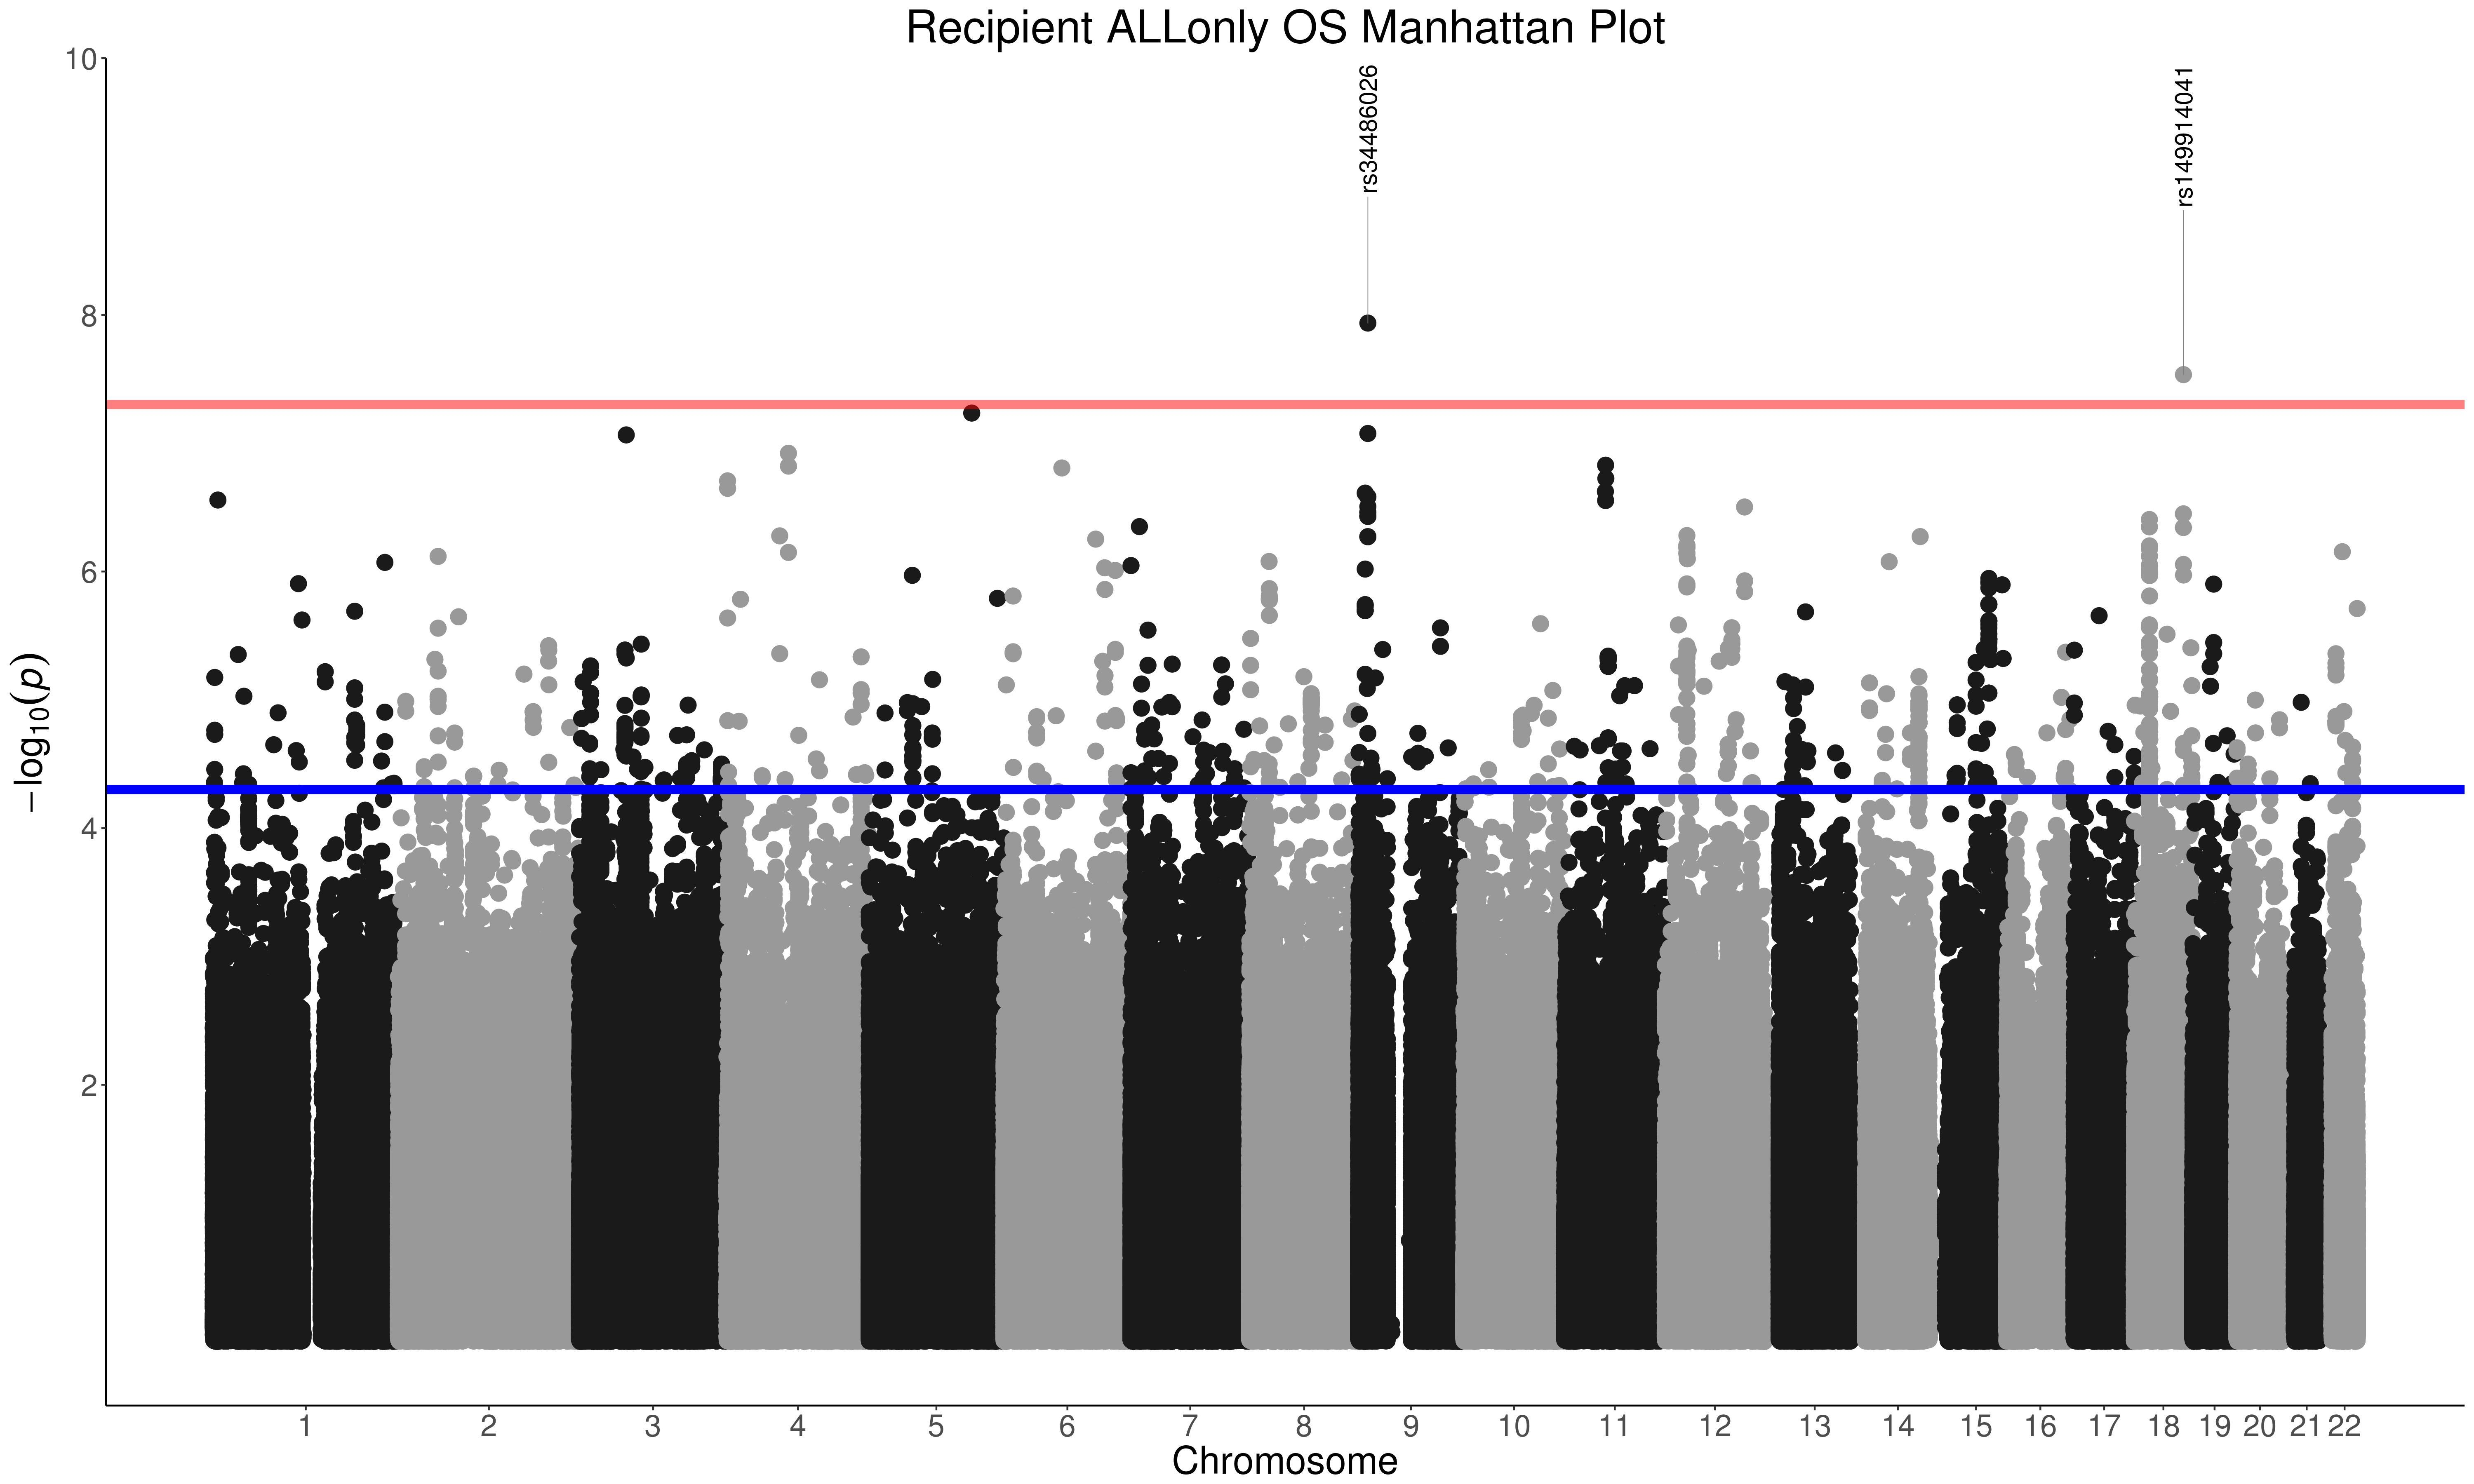
\includegraphics[width=\linewidth, height=3.5in]{~/Desktop/figures/chapter5/R_ALLonly_OS.jpeg}
    \caption[Recipient OS 1 Year Manhattan Plot]{Recipient OS 1 Year Manhattan Plot. The x-axis is chromosome 1-22 and the y-axis is the $-\log_{10}(P_{meta})$. Each dot is a SNP. The red line is genome wide significance at $P_{meta} < 5\times{10}^{-8}$. The blue line is suggestive significance at $P_{meta} < 5\times{10}^{-5}$. Labeled SNPs are associated hits that have passed genome-wide threshold.}
    \label{fig:r_os_1y}
\end{figure}

\rowcolors{2}{gray!6}{white}

\begin{table}[t]

\caption{\label{tab:unnamed-chunk-35}\label{tab:r_os_hits} DISCOVeRY-BMT Recipients Overall Survival Associations at 1-Year}
\centering
\fontsize{9}{11}\selectfont
\begin{threeparttable}
\begin{tabular}{>{\centering\arraybackslash}p{5em}|>{\centering\arraybackslash}p{5.5em}|>{\centering\arraybackslash}p{2em}|>{\centering\arraybackslash}p{10.5em}|>{\centering\arraybackslash}p{4.8em}|>{\centering\arraybackslash}p{8em}|c}
\hiderowcolors
\hline
RSID & CHR:POS & REF/ EFFECT & Ref. Panel/Cohort 1/ Cohort 2 MAF & P-value & HR (95\% CI) & INFO\\
\hline
\showrowcolors
rs34486026 & 9:12585285 & C/T & 0.0086/0.0112/0.009 & 1.159e-08 & 7 (3.59-13.67) & 0.94\\
\hline
rs149914041 & 18:65924660 & G/A & 0.0128/0.0215/0.017 & 2.923e-08 & 4.24 (2.54-7.06) & 0.90\\
\hline
\end{tabular}
\begin{tablenotes}[para]
\item All SNPs shown here are imputed. Genomic positions are GRCh37 reference genome.
\end{tablenotes}
\end{threeparttable}
\end{table}

\rowcolors{2}{white}{white}

\begin{figure}
    \centering
    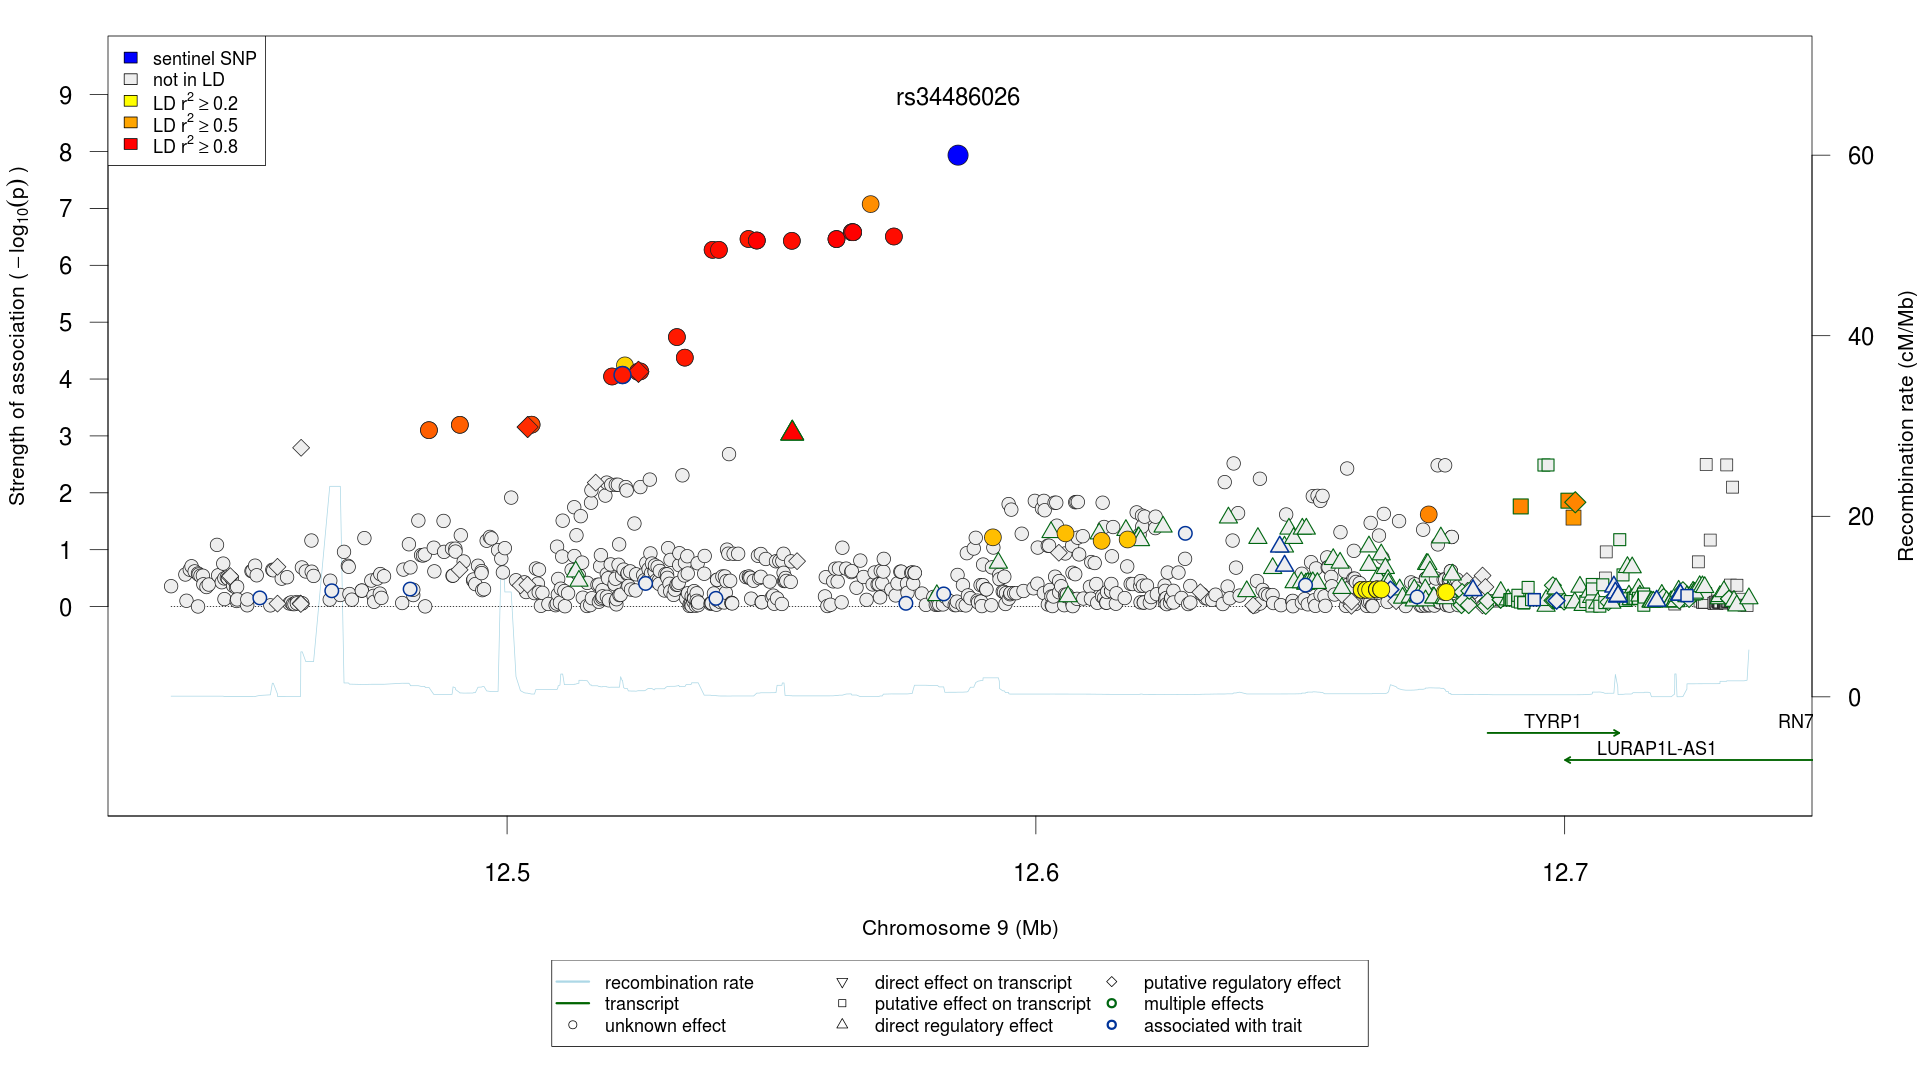
\includegraphics[width=\linewidth, height=3.5in]{~/Desktop/figures/chapter5/rs34486026_9_R_ALLonly_OS.png}
    \caption[Regional association plot of recipient SNP rs34486026 with DRM in ALL patients.]{Regional association plot of recipient SNP rs34486026 with DRM in ALL patients. The x-axis is genomic position on chromosome 2 and the y-axis is the $-\log_{10}(P_{meta})$. Sentinel SNP is rs34486026 and colored blue. The region comprises +/- 150 kb window from the sentinel SNP. The red-yellow color gradient represents LD strength. Shapes represent various regulatory or functional effects that the SNP has been reported to have in this region from independent studies.}
    \label{fig:r_os_1y_chr9reg}  
\end{figure}

\begin{figure}
    \centering
    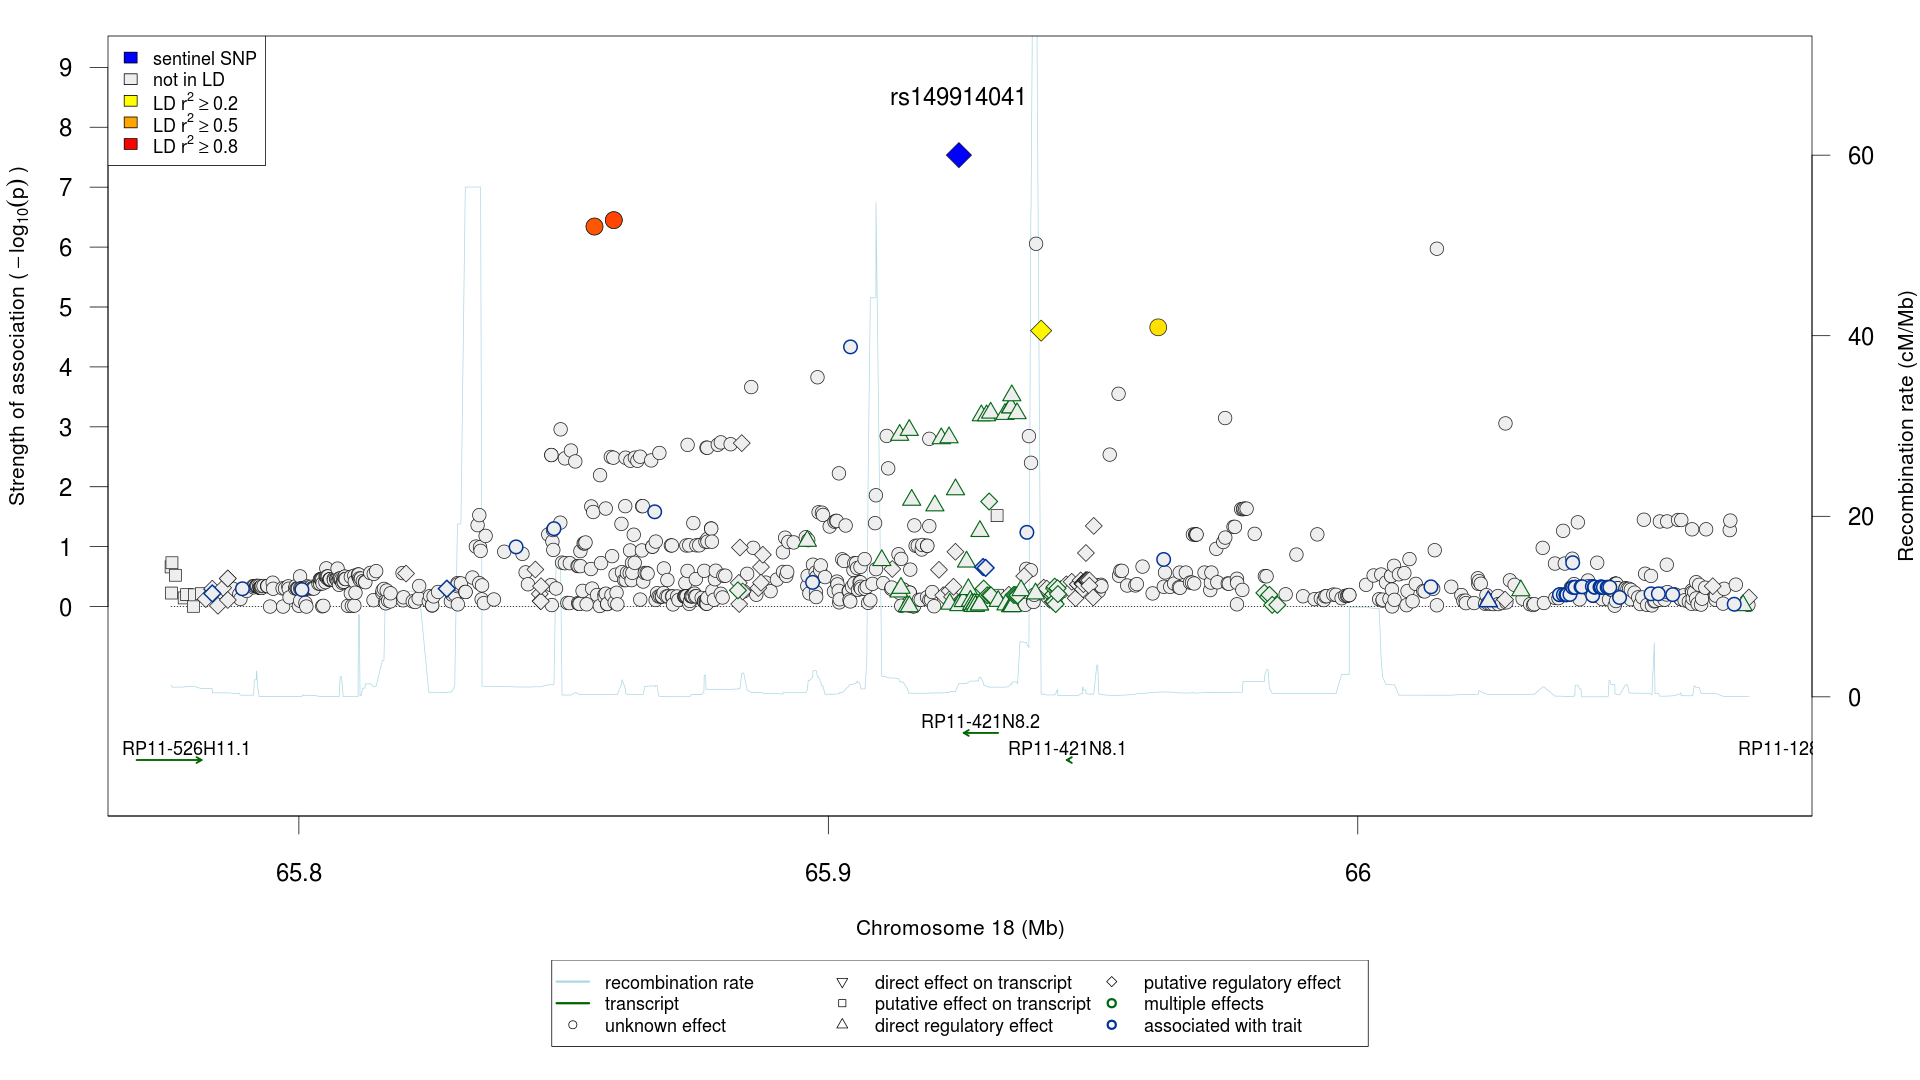
\includegraphics[width=\linewidth, height=3.5in]{~/Desktop/figures/chapter5/rs149914041_18_R_ALLonly_OS.png}
    \caption[Regional association plot of recipient SNP rs149914041 with DRM in ALL patients.]{Regional association plot of recipient SNP rs149914041 with DRM in ALL patients. The x-axis is genomic position on chromosome 2 and the y-axis is the $-\log_{10}(P_{meta})$. Sentinel SNP is rs149914041 and colored blue. The region comprises +/- 150 kb window from the sentinel SNP. The red-yellow color gradient represents LD strength. Shapes represent various regulatory or functional effects that the SNP has been reported to have in this region from independent studies.}
    \label{fig:r_os_1y_chr}  
\end{figure}

Association tests of recipient SNPs with overall survival after MUD-HSCT
revealed two loci on chromosomes 9 and 18 that reached genome-wide
significance (Figure \ref{fig:r_os_1y}; Table \ref{tab:r_os_hits}).

Association on chromosome 9 was detected for rs34486026 (Figure
\ref{fig:r_os_1y_chr9reg}), which changes binding motifs for 6 proteins
(Kheradpour and Kellis \protect\hyperlink{ref-motifs_2014}{2014}).
rs34486026 is also in LD (\(r^2=0.82\)) with rs16929156, a protein
quantitative trait loci (pQTL) for lysozyme (Lyz) protein. Lyz is a
protein with antibacterial activity found in multiple tissues and body
fluids. Associated loci on chromosome 18 was rs149914041, which alters
motif for Foxa proteins, a subclass of Fox family of transcription
factors involved in cell growth, proliferation and longevity.

We also screened recipient SNPs with suggestive OS associations
(\(P < 5 \times 10^{-5}\)) and detected two regions of interest on
chromosomes 6 and 12.

\begin{figure}
    \centering
    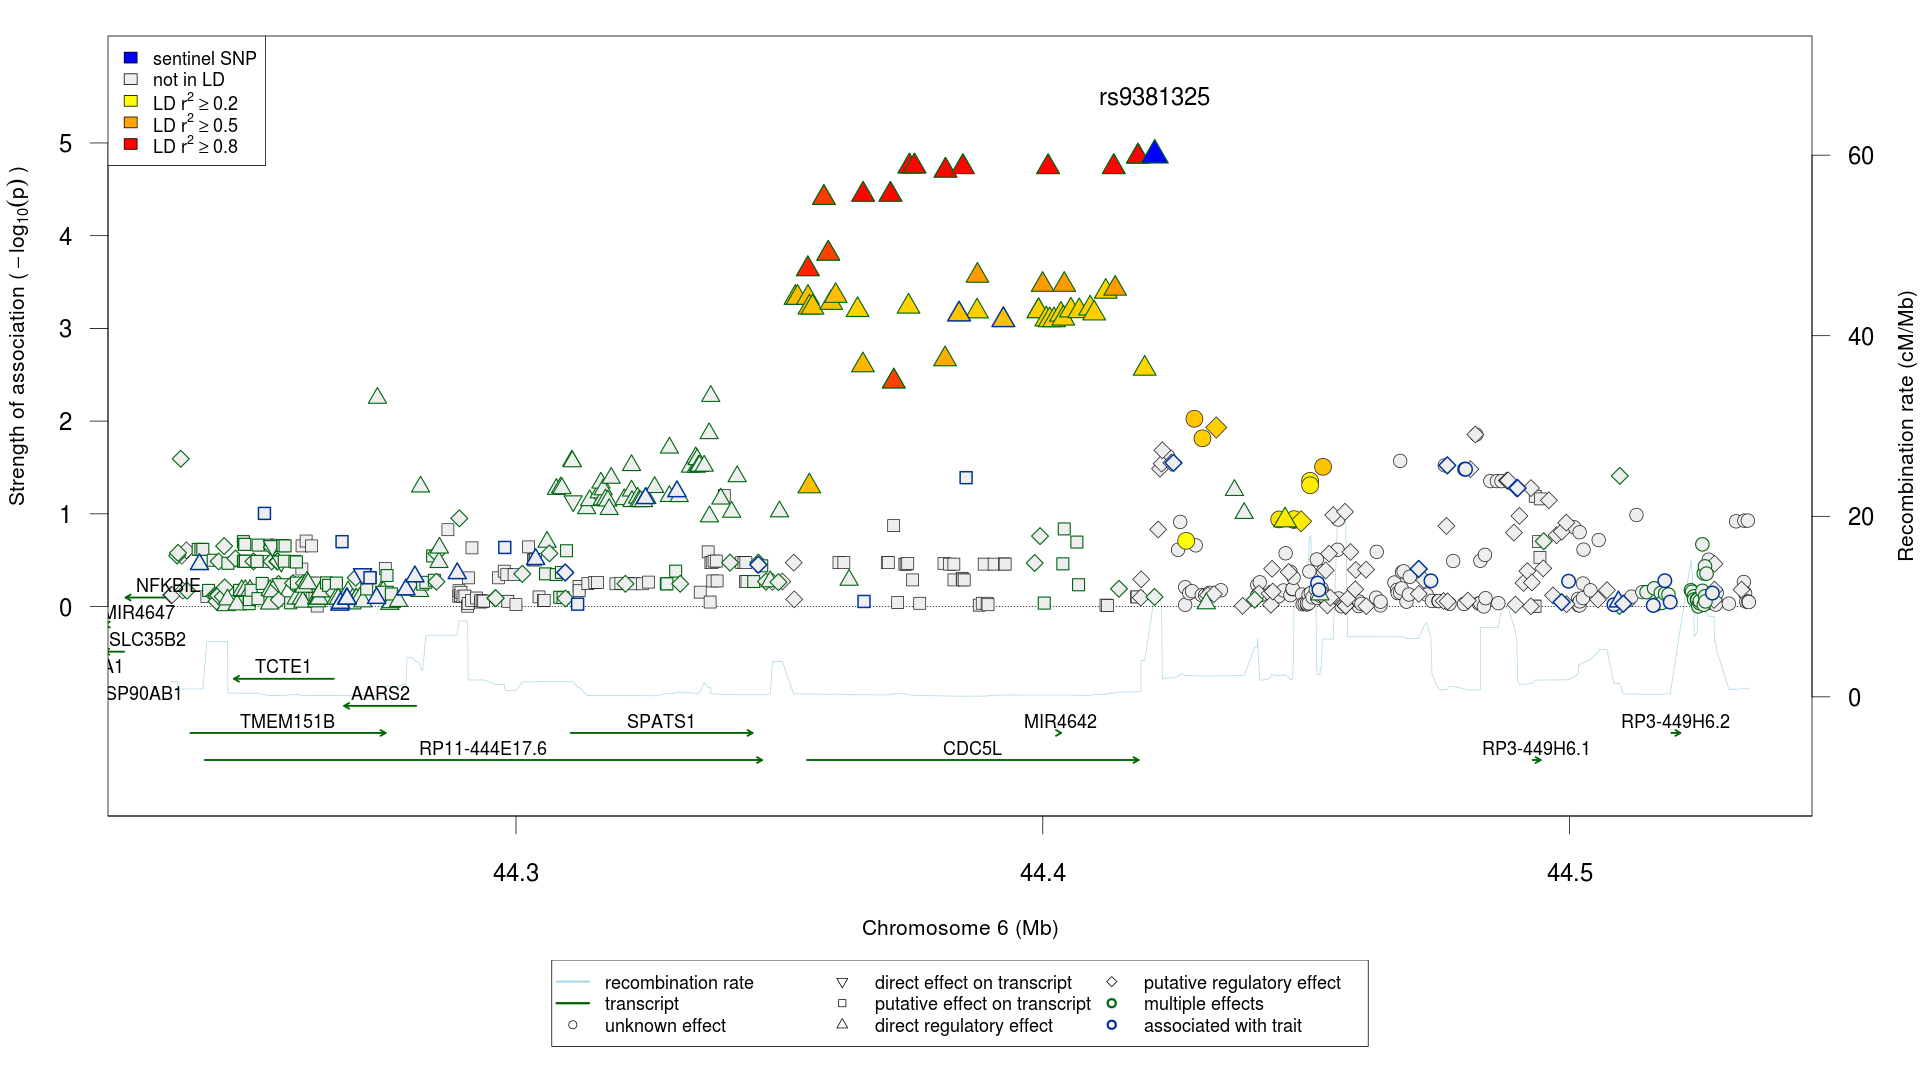
\includegraphics[width=\linewidth, height=3.5in]{~/Desktop/figures/chapter5/rs9381325_6_R_ALLonly_OS.png}
    \caption[Regional association plot of recipient SNP rs9381325 with DRM in ALL patients.]{Regional association plot of recipient SNP rs9381325 with DRM in ALL patients. The x-axis is genomic position on chromosome 2 and the y-axis is the $-\log_{10}(P_{meta})$. Sentinel SNP is rs9381325 and colored blue. The region comprises +/- 150 kb window from the sentinel SNP. The red-yellow color gradient represents LD strength. Shapes represent various regulatory or functional effects that the SNP has been reported to have in this region from independent studies.}
    \label{fig:r_os_1y_chr6}  
\end{figure}

Identified loci on chromosome 6 were eQTLs for \emph{CDCL5} gene (Figure
\ref{fig:r_os_1y_chr6}). \emph{CDCL5} encodes for Cell division cycle
5-like protein, which acts as a transcription activator. Interestingly
PRP19-CDC5L complex may also play a role in the response to DNA damage.
(Lei et al. \protect\hyperlink{ref-Lei_2000}{2000})

\subsection{Recipient SNPs Disease Related Mortality
Associations}\label{recipient-snps-disease-related-mortality-associations}

\rowcolors{2}{gray!6}{white}

\begin{table}[t]

\caption{\label{tab:unnamed-chunk-36}\label{tab:r_drm_hits} DISCOVeRY-BMT recipient genotypes associated with disease related mortality at 1-year.}
\centering
\fontsize{9}{11}\selectfont
\begin{threeparttable}
\begin{tabular}{>{\centering\arraybackslash}p{5em}|>{\centering\arraybackslash}p{5.5em}|>{\centering\arraybackslash}p{2em}|>{\centering\arraybackslash}p{10.5em}|>{\centering\arraybackslash}p{4.8em}|>{\centering\arraybackslash}p{8em}|c}
\hiderowcolors
\hline
RSID & CHR:POS & REF/ EFFECT & Ref. Panel/Cohort 1/ Cohort 2 MAF & P-value & HR (95\% CI) & INFO\\
\hline
\showrowcolors
rs4663706 & 2:238188818 & C/T & 0.0208/0.0166/0.0152 & 4.495e-09 & 7.67 (3.88-15.15) & 0.83\\
\hline
rs55671334 & 2:238194894 & C/G & 0.0212/0.0152/0.0114 & 1.609e-08 & 7.37 (3.68-14.73) & 0.93\\
\hline
rs4663709 & 2:238192685 & T/A & 0.0192/0.0151/0.0112 & 1.885e-08 & 7.32 (3.66-14.65) & 0.91\\
\hline
rs76276644 & 2:238194465 & C/T & 0.0215/0.016/0.0112 & 4.667e-08 & 6.96 (3.47-13.97) & 0.92\\
\hline
rs117522303 & 11:114863319 & C/T & 0.014/0.0141/0.0202 & 2.233e-09 & 9.88 (4.66-20.94) & 0.81\\
\hline
rs118004702 & 11:114910112 & C/T & 0.0152/0.0138/0.0221 & 4.804e-09 & 8.79 (4.25-18.2) & 0.88\\
\hline
rs149448001 & 17:15490739 & T/C & 0.0148/0.0104/0.0261 & 1.269e-10 & 9.47 (4.77-18.78) & 0.82\\
\hline
rs3865256 & 17:15489677 & C/T & 0.0185/0.0106/0.0261 & 1.444e-10 & 9.29 (4.7-18.37) & 0.83\\
\hline
rs147024703 & 17:15487520 & T/G & 0.0146/0.0106/0.0261 & 1.445e-10 & 9.29 (4.7-18.37) & 0.83\\
\hline
rs77119354 & 17:15495401 & A/G & 0.017/0.011/0.0266 & 2.015e-09 & 7.35 (3.83-14.12) & 0.84\\
\hline
\end{tabular}
\begin{tablenotes}[para]
\item All SNPs shown are imputed. Genomic positions are GRCh37 reference genome.
\end{tablenotes}
\end{threeparttable}
\end{table}

\rowcolors{2}{white}{white}

\begin{figure}
    \centering
    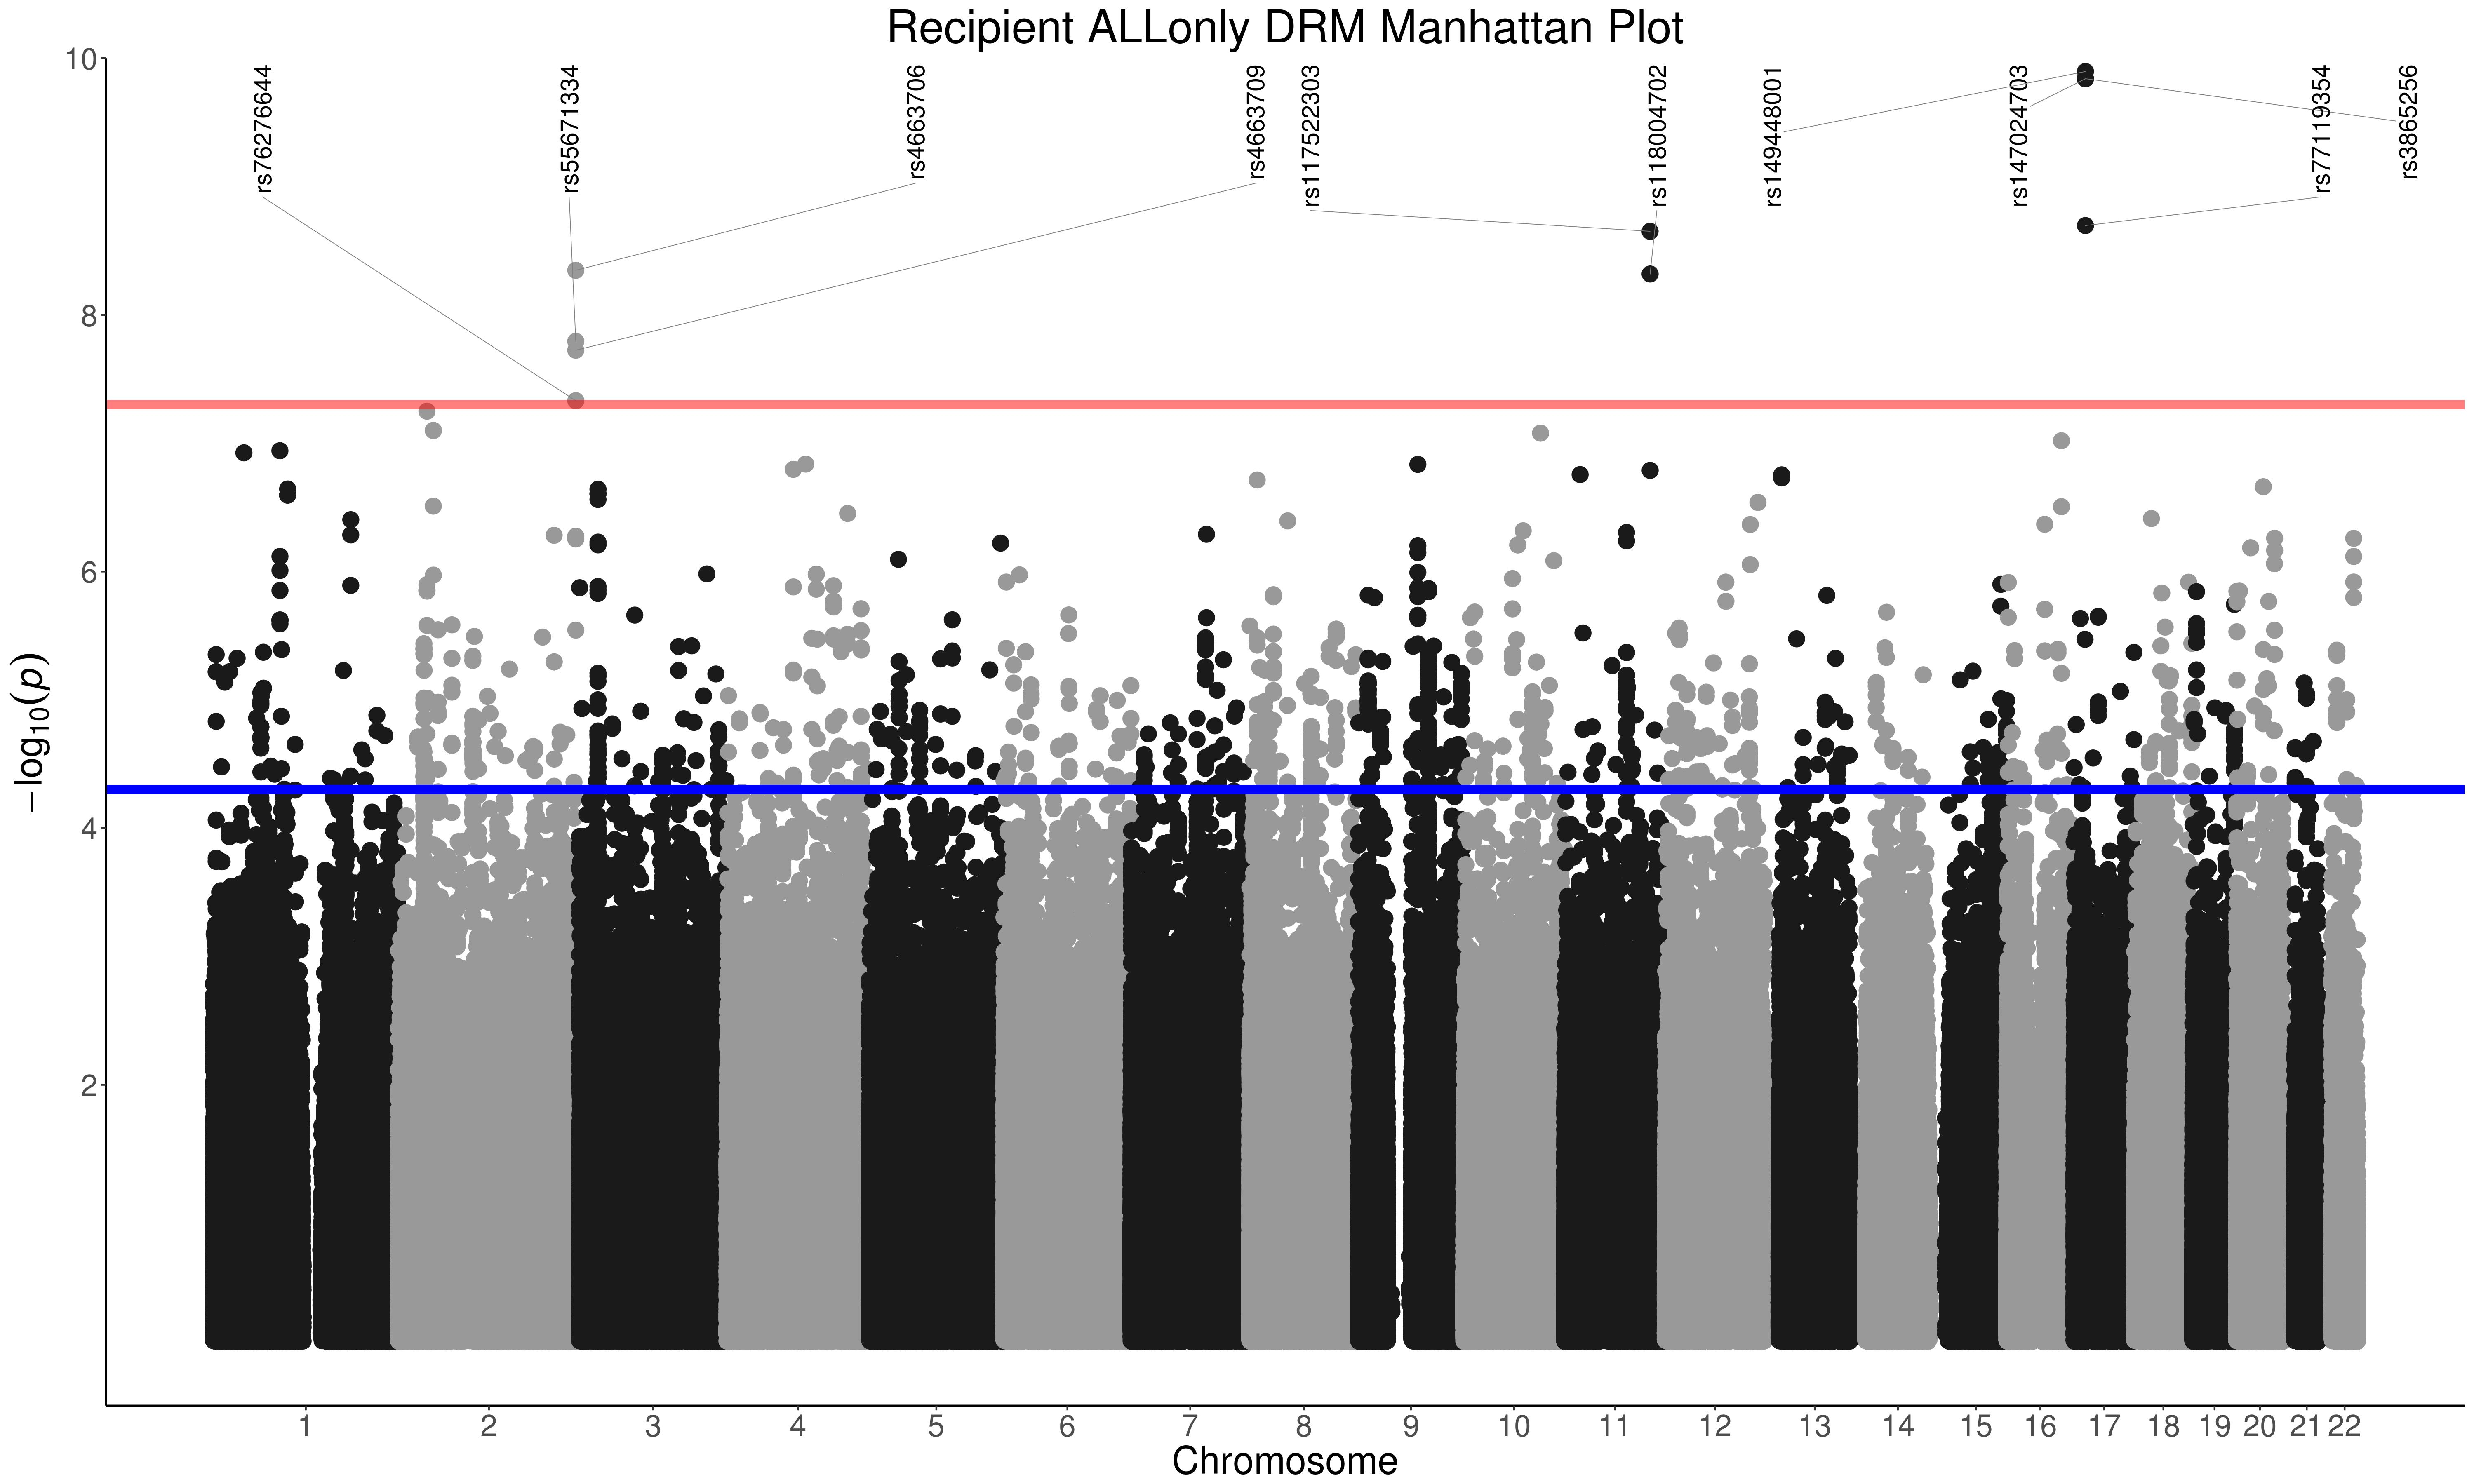
\includegraphics[width=\linewidth, height=3.5in]{~/Desktop/figures/chapter5/R_ALLonly_DRM.jpeg}
    \caption[Manhattan Plot of Recipient ALL DRM GWAS.]{Manhattan Plot of Recipient ALL DRM GWAS. The x-axis is chromosome 1-22 and the y-axis is the $-\log_{10}(P_{meta})$. Each dot is a SNP. The red line is genome wide significance at $P_{meta} < 5\times{10}^{-8}$. The blue line is suggestive significance at $P_{meta} <  5\times{10}^{-5}$. Labeled SNPs are associated hits that have passed genome-wide threshold.}
    \label{fig:r_drm_1y}  
\end{figure}

\begin{figure}
    \centering
    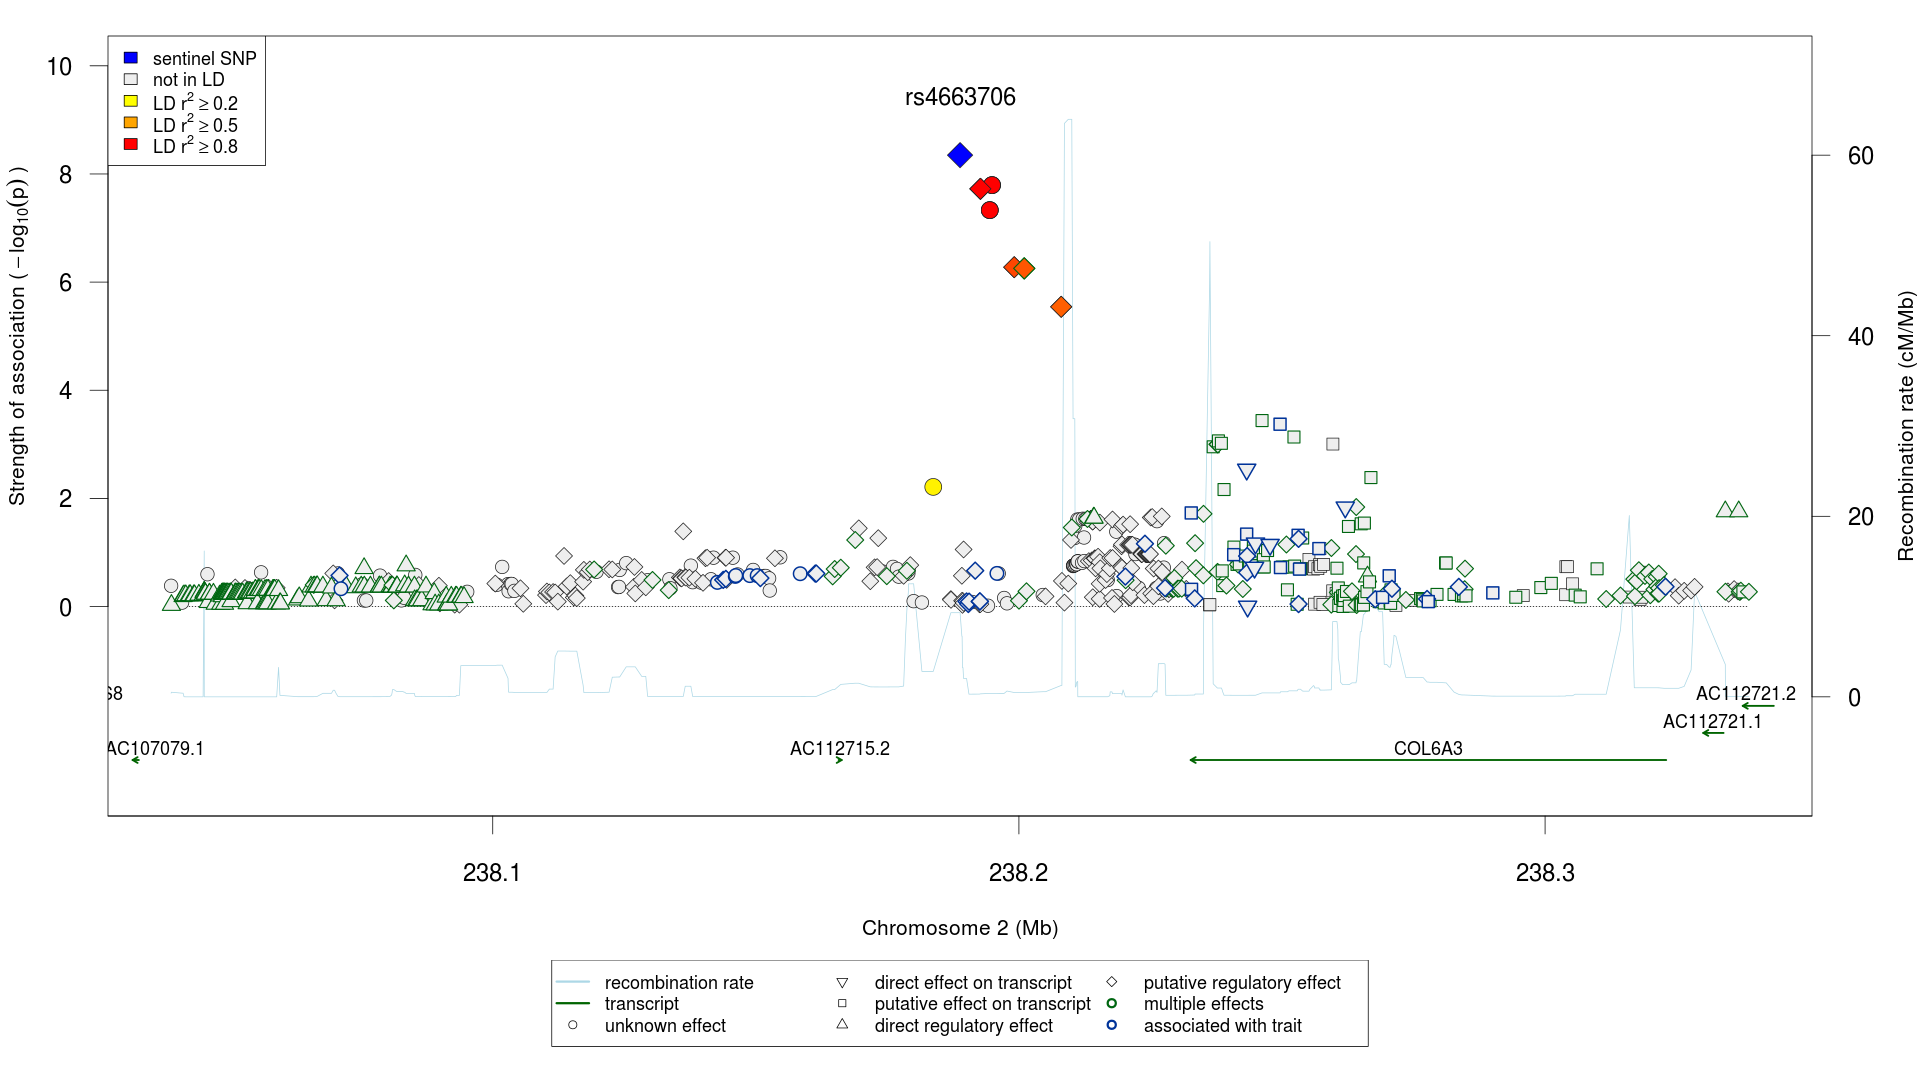
\includegraphics[width=\linewidth, height=3.5in]{~/Desktop/figures/chapter5/rs4663706_2_R_ALLonly_DRM.png}
    \caption[Regional association plot of recipient SNP rs4663706 with DRM in ALL patients.]{Regional association plot of recipient SNP rs4663706 with DRM in ALL patients. The x-axis is genomic position on chromosome 2 and the y-axis is the $-\log_{10}(P_{meta})$. Sentinel SNP is rs4663706 and colored blue. The region comprises +/- 150 kb window from the sentinel SNP. The red-yellow color gradient represents LD strength. Shapes represent various regulatory or functional effects that the SNP has been reported to have in this region from independent studies.}
    \label{fig:r_drm_1y_chr2reg1}  
\end{figure}

We found genome-wide recipient SNP associations
(\(P_{meta} < 5\times{10}^{-8}\)) with DRM on chromosomes 2, 11, and 17
(Figure \ref{fig:r_drm_1y}).

Among the genome-wide associated (GWA) SNPs on chromosome 2, rs4663706
had the strongest association (Table \ref{tab:r_drm_hits}). Three SNPs
(rs55671334, rs4663709, rs76276644) in the region are in LD with
rs4663706 at \(r^2>0.8\). These SNPs are located in the upstream of
\emph{COL6A3} gene and this intergenic region has been predicted as an
enhancer region in multiple tissues, including primary hematopoietic
stem cells by Roadmap Epigenome project (Figure
\ref{fig:r_drm_1y_chr2reg1}). It is important to note however, that all
four SNPs including rs4663706 are imputed (\(\text{INFO} > 0.8\)).
Furthermore, while rs55671334, rs4663709, rs76276644 had genome-wide
significant \(P_{meta}\) values, (Figure \ref{fig:r_drm_1y}) the
associations appear to be driven by cohort 1, as
\(P_{\text{cohort2}} > 0.1\) (Table \ref{tab:r_drm_hits}). Thus,
p-values in cohort 2 weaken confidence in the genome-wide association in
this region.

\begin{figure}
    \centering
    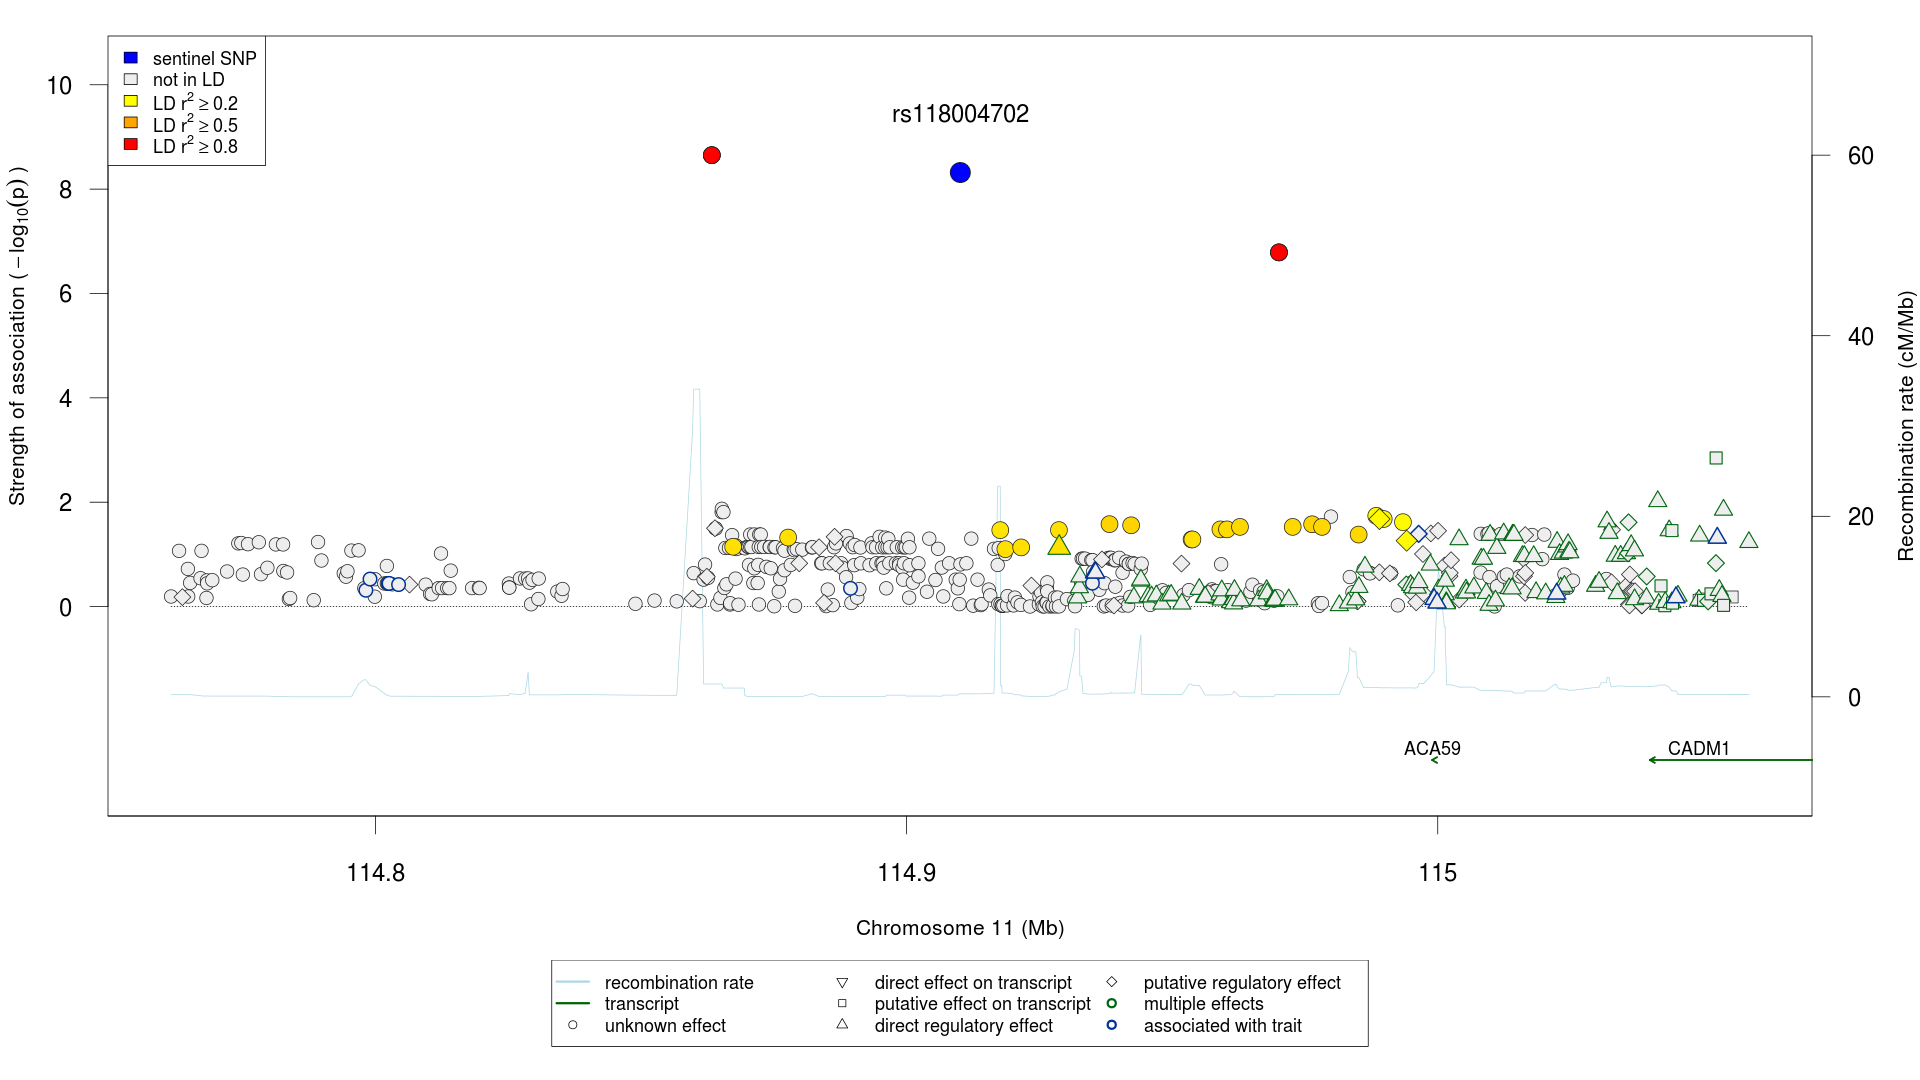
\includegraphics[width=\linewidth, height=3.5in]{~/Desktop/figures/chapter5/rs118004702_11_R_ALLonly_DRM.png}
    \caption[Regional association plot of recipient SNP rs118004702 with DRM in ALL patients.]{Regional association plot of recipient SNP rs118004702 with DRM in ALL patients. The x-axis is genomic position on chromosome 2 and the y-axis is the $-\log_{10}(P_{meta})$. Sentinel SNP is rs118004702 and colored blue. The region comprises +/- 150 kb window from the sentinel SNP. The red-yellow color gradient represents LD strength. Shapes represent various regulatory or functional effects that the SNP has been reported to have in this region from independent studies.}
    \label{fig:r_drm_1y_chr11reg}  
\end{figure}

The region on chromosome 11, includes two genome-wide associated SNPs,
rs118004702 and rs117517252 (\(r^2=0.94\)) (Table \ref{tab:r_drm_hits};
Figure \ref{fig:r_drm_1y}; Figure \ref{fig:r_drm_1y_chr11reg}). ENCODE
ChIP-Seq experiments report that SNPs in this region alter regulatory
motifs on \emph{HNF4} and \emph{TAL1} (Kheradpour and Kellis
\protect\hyperlink{ref-motifs_2014}{2014}). \emph{TAL1} has been
reported as an oncogenic transcription factor in T-cell ALL subtype
(Sanda and Leong \protect\hyperlink{ref-sanda_2017}{2017}).

\begin{figure}
    \centering
    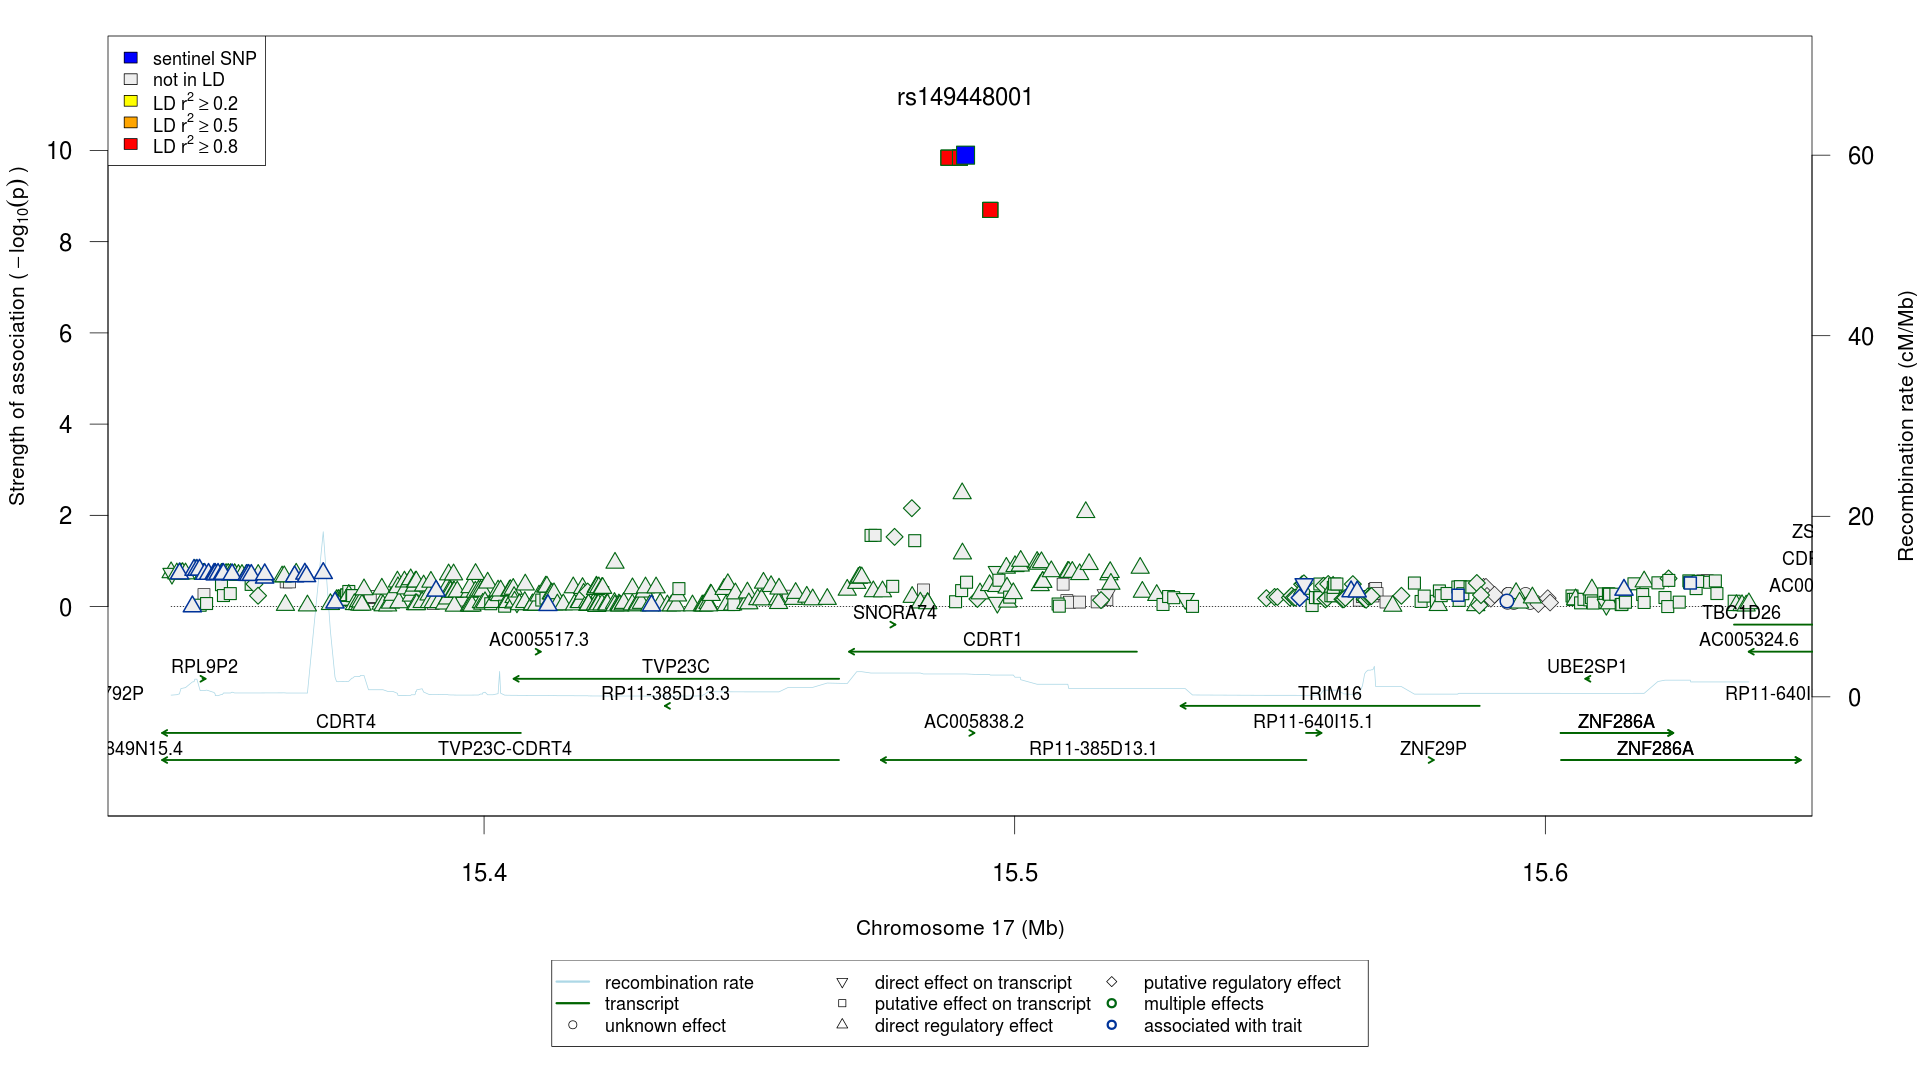
\includegraphics[width=\linewidth, height=3.5in]{~/Desktop/figures/chapter5/rs149448001_17_R_ALLonly_DRM.png}
    \caption[Regional association plot of recipient SNP rs149448001 with DRM in ALL patients.]{Regional association plot of recipient SNP rs149448001 with DRM in ALL patients. The x-axis is genomic position on chromosome 2 and the y-axis is the $-\log_{10}(P_{meta})$. Sentinel SNP is rs149448001 and colored blue. The region comprises +/- 150 kb window from the sentinel SNP. The red-yellow color gradient represents LD strength. Shapes represent various regulatory or functional effects that the SNP has been reported to have in this region from independent studies.}
    \label{fig:r_drm_1y_chr17reg}  
\end{figure}

\begin{figure}
    \centering
    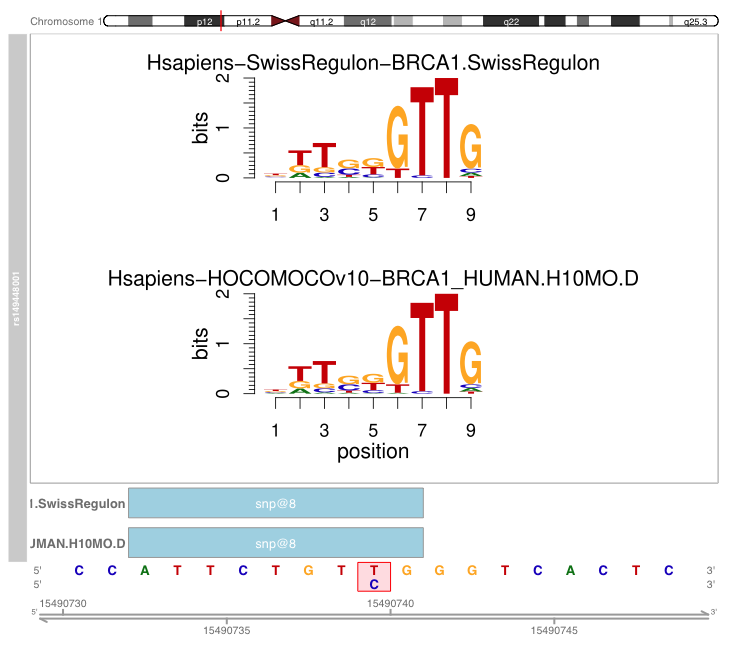
\includegraphics[width=\linewidth, height=3.5in]{~/Desktop/figures/chapter5/rs149448001_motif.png}
    \caption[Recipient DRM Chromosome 17 rs149448001 motif.]{Recipient DRM Chromosome 17 rs149448001 motif. A schematic of chromosome 17 is at the top. The red vertical line it the genomic location that the of this motif. The two panels show BRCA1 binding motif on chromosome 7 from two different human motif databases. rs149448001 is located at position 8 from T to C. The coordinate is highly predicted to be a T, and therefore a C allele will likely alter the binding properties of proteins to this region.}
    \label{fig:r_drm_motif}  
\end{figure}

Chromosome 17 has four recipient SNPs (rs149448001, rs3865256,
rs147024703, rs77119354) associated with DRM within the first year
transplant (Table \ref{tab:r_drm_hits}; Figure \ref{tab:r_drm_hits};
Figure \ref{fig:r_drm_1y_chr17reg}). All four SNPs are located in the
intronic region of CDRT1 and alter binding motifs for various proteins
known to play important roles in leukemias or other cancers (i.e.
\emph{BRCA1}, \emph{CDX}, \emph{E2A}, \emph{STAT} and \emph{GATA}
families) (Perez-Andreu et al.
\protect\hyperlink{ref-PerezAndreu_2015}{2015}). The SNP rs149448001 had
the strongest association in this region and significantly changes the
binding motif of \emph{BRCA1}, a well known tumor suppressor. In fact
rs149448001 changes the only unambiguous 8th position in the motif from
T to C (Figure \ref{fig:r_drm_motif}; S. G. Coetzee, Coetzee, and
Hazelett (\protect\hyperlink{ref-motifbreakr}{2015})).The Roadmap
Epigenome Project, places one of the associated SNPs, rs77119354, in an
enhancer region in almost all primary T-cell and hematopoietic stem cell
lines (L. D. Ward and Kellis \protect\hyperlink{ref-haploreg}{2015}).

\begin{figure}
    \centering
    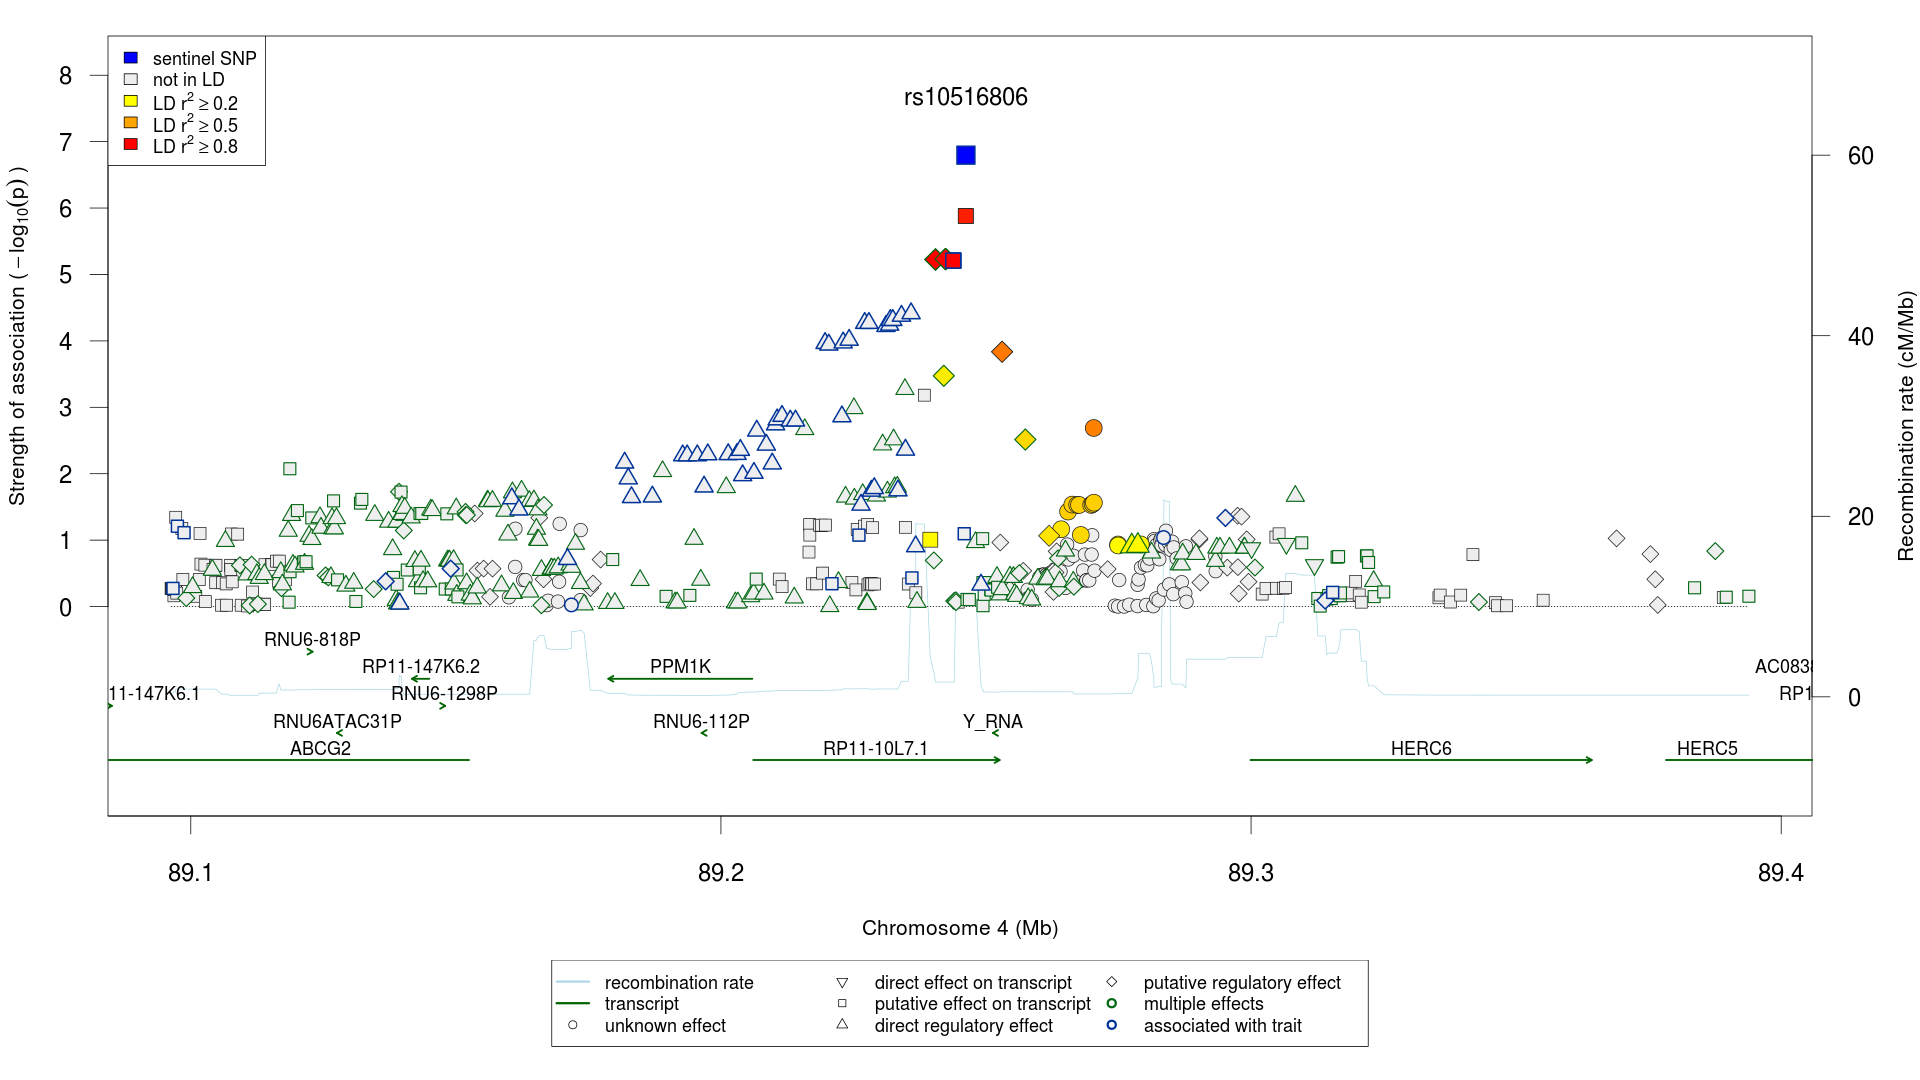
\includegraphics[width=\linewidth, height=3.5in]{~/Desktop/figures/chapter5/rs10516806_4_R_ALLonly_DRM.png}
    \caption[Regional association plot of recipient SNP rs10516806 with DRM in ALL patients.]{Regional association plot of recipient SNP rs10516806 with DRM in ALL patients. The x-axis is genomic position on chromosome 2 and the y-axis is the $-\log_{10}$(P-value). Sentinel SNP is rs10516806 and colored blue. The region comprises +/- 150 kb window from the sentinel SNP. The red-yellow color gradient represents LD strength. Shapes represent various regulatory or functional effects that the SNP has been reported to have in this region from independent studies.}
    \label{fig:r_drm_1y_chr4reg}  
\end{figure}

We also inspected recipient SNPs with suggestive DRM associations
(\(P < 5\times{10}^{-5}\)) for previously reported regulatory function.
This revealed a region on chromosome 4 where blood metabolite levels
associations (rs10022462; Shin et al.
\protect\hyperlink{ref-shin_2014}{2014}) (Figure
\ref{fig:r_drm_1y_chr4reg}) had been reported. The blood metabolite GWAS
hit is in LD with rs10516806 (\(r^{2} = 0.82\);
\(P=1.6\times{10}^{-7}\); HR: 0.474 {[}0.359-0.627{]} for T allele) in
recipient DRM. Rs10516806 is in perfect LD (\(r^2=1\)) with rs2869930
which has been identified as protein bound in ChIP-Seq experiments for
\emph{FOXA1} (in liver cell line Hep G2) and \textit{ER$\alpha$} (also
known as \emph{NR3A1}; in T-47D human breast cancer cells) (ENCODE
Project Consortium \protect\hyperlink{ref-encode_2012}{2012}).
\emph{FOXA1} is a transcription factor that belongs to the \emph{FOX}
family -- of which another member of this family, \emph{FOXP1}, when
downregulated is associated with deficient B-cells (H. Hu et al.
\protect\hyperlink{ref-hu_2006}{2006}; Wlodarska et al.
\protect\hyperlink{ref-Wlodarska_2005}{2005}). \emph{FOXA1} and
\emph{FOXP1} are transcription factors that are known to modulate
activity of \textit{ER$\alpha$} in breast cancer (Ijichi et al.
\protect\hyperlink{ref-Ijichi_2013}{2013}). It may be plausible to
further interrogate \emph{FOXA1} status in patients who die from their
original disease.

rs10516806 and SNPs that are in LD (\(r^2\) \textgreater{} 0.82) have
enhancer and promoter histone marks in blood and transplant related
tissues (i.e.~skin, GI). Rs10516806 is associated with chromatin marks
(H3K4me1 for primary T cells from peripheral blood). SNPs in this region
alter regulatory motifs on \emph{CEBPB} family genes, \emph{ZPF410},
\emph{FOXP3}, \emph{HOXD8}, and \emph{PAX5}. \emph{ZPF410} is a
\emph{PAX5} activated gene (S. Yang et al.
\protect\hyperlink{ref-yang_2015}{2015}). \emph{PAX5} encodes for
transcription factors that are essential for progression of adult B
lymphoiesis from early B cell progenitor cells (Nutt et al.
\protect\hyperlink{ref-nutt_1998}{1998}; S. Shah et al.
\protect\hyperlink{ref-shah_2013}{2013}). This region has been reported
to be associated to gene expression or quantitative traits in several
studies. The locus rs10516806 is an eQTL and effects \emph{PPM1K} gene
expression in liver and breast cell lines (Q. Li et al.
\protect\hyperlink{ref-li_2014}{2014}). Furthermore, a recent study
\emph{PPM1K} is involved in amino acid catabolism in HSCs and plays a
major role in maintaining stem cell status and HSC repopulation in mice
bone marrow (X. Liu et al. \protect\hyperlink{ref-Liu_2018}{2018}). This
study suggests that \emph{PPM1K} deletion in murine models improve
survival (X. Liu et al. \protect\hyperlink{ref-Liu_2018}{2018}).

While this could manifest different phenotypes in humans, it suggests
that investigating the direction (risk or protective) rs10516806 alters
\emph{PPM1K} gene expression is reasonable.

\subsection{Exploratory analyses: Recipient SNP associations with Organ
Failure}\label{exploratory-analyses-recipient-snp-associations-with-organ-failure}

\begin{figure}
    \centering
    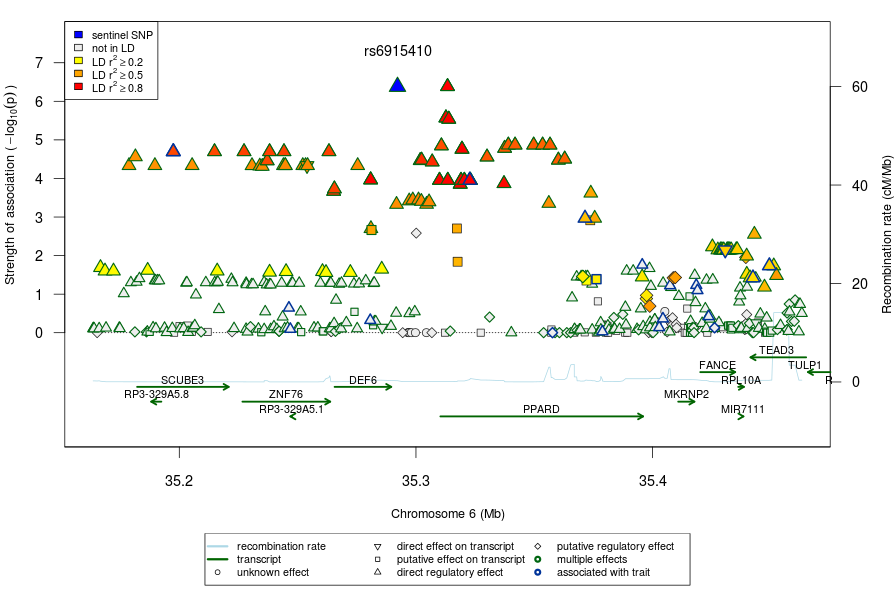
\includegraphics[width=\linewidth, height=3.5in]{~/Desktop/figures/chapter5/r_of_1y_gwas_hit.png}
    \caption[Organ failure in recipient on chromosome 6.]{Organ failure in recipient on chromosome 6. Sentinel SNP is rs6915410 and colored blue. The region comprises +/- 150 kb window from the sentinel SNP. The red-yellow color gradient represents LD strength. Shapes represent different effects that the SNP has been reported to have in this region from independent studies.}
    \label{fig:r_of_1y}  
\end{figure}

While more recipients died due to transplant in the first year compared
to death due to disease (Table \ref{tab:all_event_props}), no
genome-wide associations with recipient SNPs were uncovered from TRM
survival analyses (Manhattan Plot not shown).

However, upon when we scanned suggestive associations organ failure in
DISCOVeRY-BMT, we identified rs6915410 (\(P = 4.17\times{10}^{-7}\); HR:
4.64 {[}2.56-8.38{]}; C effect allele) on chromosome 6 as an interesting
locus for death by organ failure (OF) in recipients. This SNP is in a
very active region, where many SNPs that are in moderate to high LD have
direct regulatory effects on \emph{DEF6} and \emph{PPARD} (Figure
\ref{fig:r_of_1y}). In addition to rs7744392 being \emph{DEF6} eQTL in
peripheral blood monocytes (Zeller et al.
\protect\hyperlink{ref-Zeller_2010}{2010}) and blood (Fehrmann et al.
\protect\hyperlink{ref-Fehrmann_2011}{2011}), it is an eQTL for
\emph{MPO} in peripheral monocytes (Zeller et al.
\protect\hyperlink{ref-Zeller_2010}{2010}) as well. These eQTLs were
identified in lymphoblastoid and whole blood derived cell lines (Zeller
et al. \protect\hyperlink{ref-Zeller_2010}{2010}; Fehrmann et al.
\protect\hyperlink{ref-Fehrmann_2011}{2011}). Blood is the most abundant
tissue that has histone marks on enhancers and promoter regions for
rs6915410 and corresponding correlated SNPs (L. D. Ward and Kellis
\protect\hyperlink{ref-haploreg}{2015}). Experimental ChIP-seq studies
have shown that \textit{ER$\alpha$} protein binds to this region.
Notably, this region has evidence of altered regulatory motifs including
known leukemia genes \emph{E2A}, \emph{AR3A}, and \emph{CEBPB},
\emph{FOXO}, \emph{GATA}, \emph{STAT} families (Iacobucci and Mullighan
\protect\hyperlink{ref-Iacobucci_2017}{2017}).

\subsection{Post-HSCT Associations with Donor
SNPs}\label{post-hsct-associations-with-donor-snps}

All eight patient outcomes (DRM, TRM, OS, PFS, REL, GVHD, INF and OF) in
ALL patients were tested for association with their matched unrelated
donors SNPs. We detected genome-wide associated regions with OS, DRM,
TRM and GVHD outcomes. Identifying such donor SNPs can be helpful in
providing insight on genes and pathways involved in post-transplant
events. More importantly upon rigorous replication, these SNPs can help
clinicians improve donor selection and ultimately post-transplant
survival outcomes.

\subsection{Donor SNPs Associated with Recipient Overall
Survival}\label{donor-snps-associated-with-recipient-overall-survival}

\begin{figure}
    \centering
    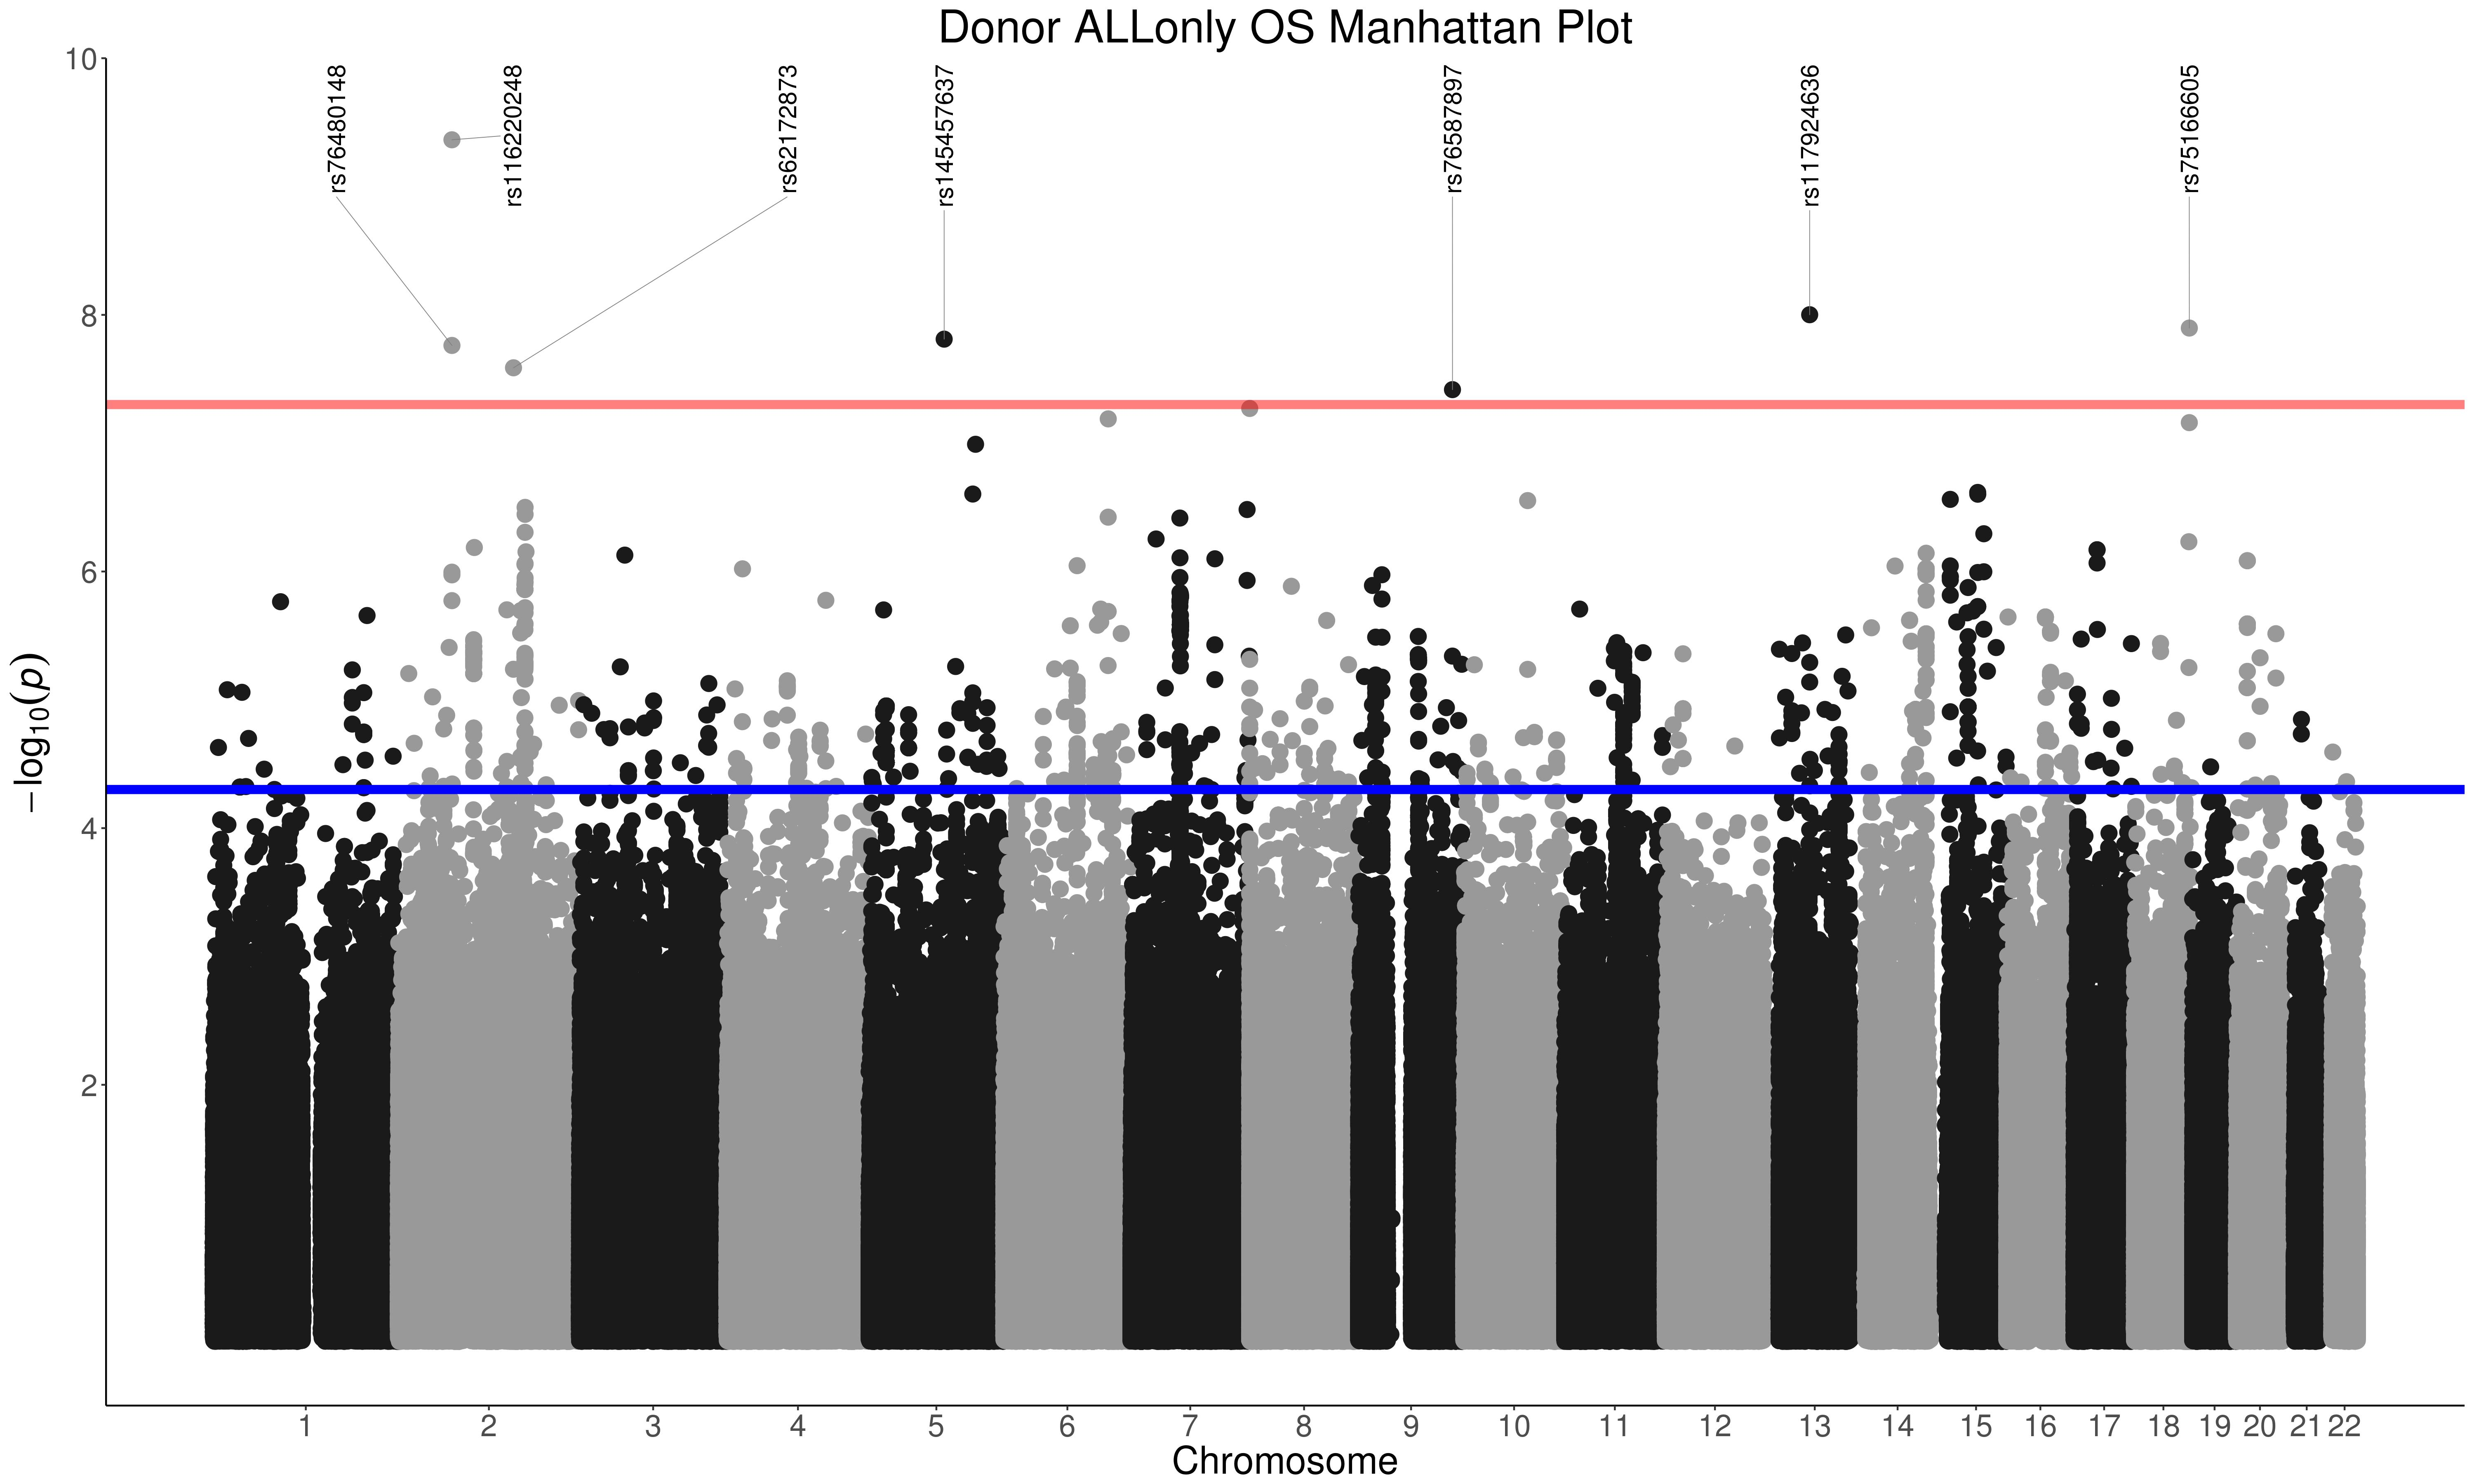
\includegraphics[width=\linewidth, height=3.5in]{~/Desktop/figures/chapter5/D_ALLonly_OS.jpeg}
    \caption[Manhattan Plot of Donor ALL OS GWAS.]{Manhattan Plot of Donor ALL OS GWAS. The x-axis is chromosome 1-22 and the y-axis is the $-\log_{10}(P_{meta})$. Each dot is a SNP. The red line is genome wide significance at $P_{meta} < 5\times{10}^{-8}$. The blue line is suggestive significance at $P < 5\times{10}^{-5}$. Labeled SNPs are associated hits that have passed genome-wide threshold.}
    \label{fig:d_os_1y}  
\end{figure}

\rowcolors{2}{gray!6}{white}

\begin{table}[t]

\caption{\label{tab:unnamed-chunk-39}\label{tab:d_os_hits} DISCOVeRY-BMT Donor SNPs Associated to Recipient Overall Survival at 1-Year}
\centering
\fontsize{9}{11}\selectfont
\begin{threeparttable}
\begin{tabular}{>{\centering\arraybackslash}p{5em}|>{\centering\arraybackslash}p{5.5em}|>{\centering\arraybackslash}p{2em}|>{\centering\arraybackslash}p{10.5em}|>{\centering\arraybackslash}p{4.8em}|>{\centering\arraybackslash}p{8em}|c}
\hiderowcolors
\hline
RSID & CHR:POS & REF/ EFF & Ref. Panel/Cohort 1/ Cohort 2 MAF & P-value & HR (95\% CI) & INFO\\
\hline
\showrowcolors
rs116220248 & 2:71934021 & C/A & 0.0055/0.0065/0.0054 & 4.322e-10 & 12.57 (5.68-27.84) & 0.87\\
\hline
rs76480148 & 2:71935916 & A/G & 0.0077/0.0096/0.0099 & 1.731e-08 & 6.96 (3.54-13.65) & 0.85\\
\hline
rs62172873 & 2:154571794 & G/C & 0.007/0.0076/0.0121 & 2.585e-08 & 8.25 (3.92-17.35) & 0.87\\
\hline
rs145457637 & 5:100869997 & G/T & 0.0123/0.0137/0.0204 & 1.546e-08 & 5.73 (3.13-10.48) & 0.82\\
\hline
rs76587897 & 9:126156904 & T/C & 0.0227/0.0259/0.0196 & 3.826e-08 & 3.82 (2.37-6.16) & 0.91\\
\hline
rs117924636 & 13:60333297 & A/G & 0.0131/0.01/0.007 & 9.976e-09 & 7.13 (3.64-13.97) & 0.89\\
\hline
rs75166605 & 18:73806958 & G/A & 0.0067/0.0065/0.0199 & 1.267e-08 & 8.68 (4.12-18.26) & 0.96\\
\hline
\end{tabular}
\begin{tablenotes}[para]
\item All SNPs shown here are imputed. Genomic positions are GRCh37 reference genome. REF is reference allele and EFF is effect allele.
\end{tablenotes}
\end{threeparttable}
\end{table}

\rowcolors{2}{white}{white}

\begin{figure}
    \centering
    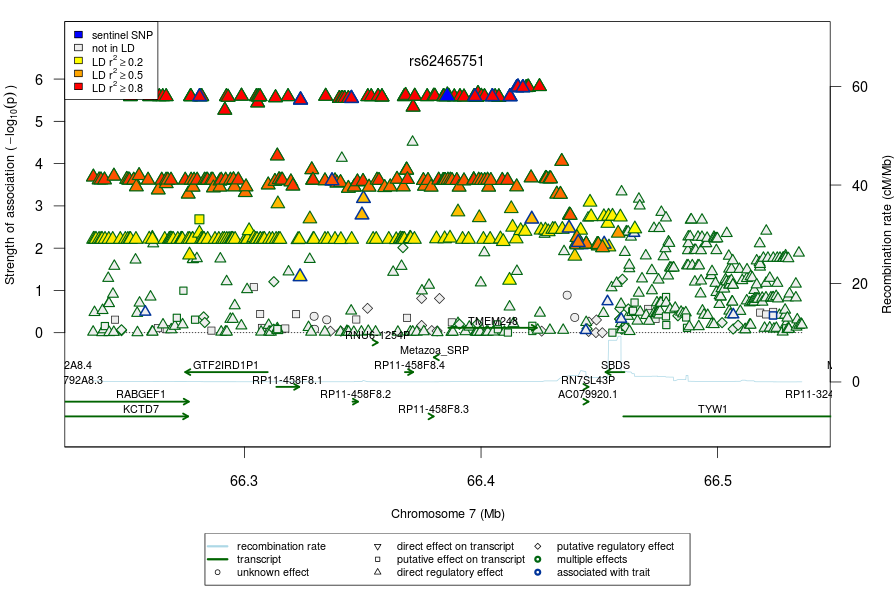
\includegraphics[width=\linewidth, height=3.5in]{~/Desktop/figures/chapter5/rs62465751_7_D_ALLonly_OS.png}
    \caption[Donor OS Region Chromosome 7.]{Donor OS Region Chromosome 7. Sentinel SNP is rs62465751 and colored blue. The region comprises +/- 150 kb window from the sentinel SNP. The red-yellow color gradient represents LD strength. Shapes represent different effects that the SNP has been reported to have in this region from independent studies.}
    \label{fig:d_os_chr7}  
\end{figure}

Donor SNPs were associated to recipient overall survival (OS) on
chromosomes 2, 5, 9, 13, and 18 (Figure \ref{fig:d_os_1y} and Table
\ref{tab:d_os_hits}).

There are two associated regions on chromosome 2 (near 71Mb and 154 Mb).
The former has two associated SNPs in perfectly correlated (rs116220248,
rs76480148), both of these SNPs are in perfect LD with a SNP that has
protein binding evidence for CEBPB, a well known leukemia target gene
(Akasaka et al. \protect\hyperlink{ref-Akasaka_2007}{2007}; Guerzoni et
al. \protect\hyperlink{ref-Guerzoni_2006}{2006}). The other region
(\(\approx\) 154 Mb region) does not have any noteworthy functional
effects. Similarly, the regions on 5, 9, 13, and 18 also provided little
evidence of having any known eQTLs, promoters Histones, or relevant
alterations to cancer related motifs (L. D. Ward and Kellis
\protect\hyperlink{ref-haploreg}{2015}; Arnold et al.
\protect\hyperlink{ref-snipa}{2015}).

Upon screening suggestive associations of donor SNPs with patient OS, we
detected rs62465751, a highly regulatory SNP located on chromosome 7,
upstream of \emph{TMEM248} (Figure \ref{fig:d_os_chr7}). This location
encompassing rs62465751 has been predicted to be an active transcription
start site in almost all cell lines included in Roadmap Epigenome
project. Consequently, rs62465751 was detected for 60 eQTL associations,
involving multiple genes across multiple tissues included in GTEx
project. rs62465751 belongs to a LD block consisting of 73 SNPs
(\(r^2>0.8\)), 22 of which located in the intronic region of
\emph{TMEM248}. SNPs in this LD block alter more than 22 binding motifs
and are all reported eQTLs for various tissues, including CEU ancestry
lymphoblastoid cell lines (Stranger et al.
\protect\hyperlink{ref-stranger_2007}{2007}; Lappalainen et al.
\protect\hyperlink{ref-Lappalainen_2013}{2013}).

\subsection{Donor SNPs Associated with Recipient Disease Related
Mortality}\label{donor-snps-associated-with-recipient-disease-related-mortality}

\begin{figure}
    \centering
    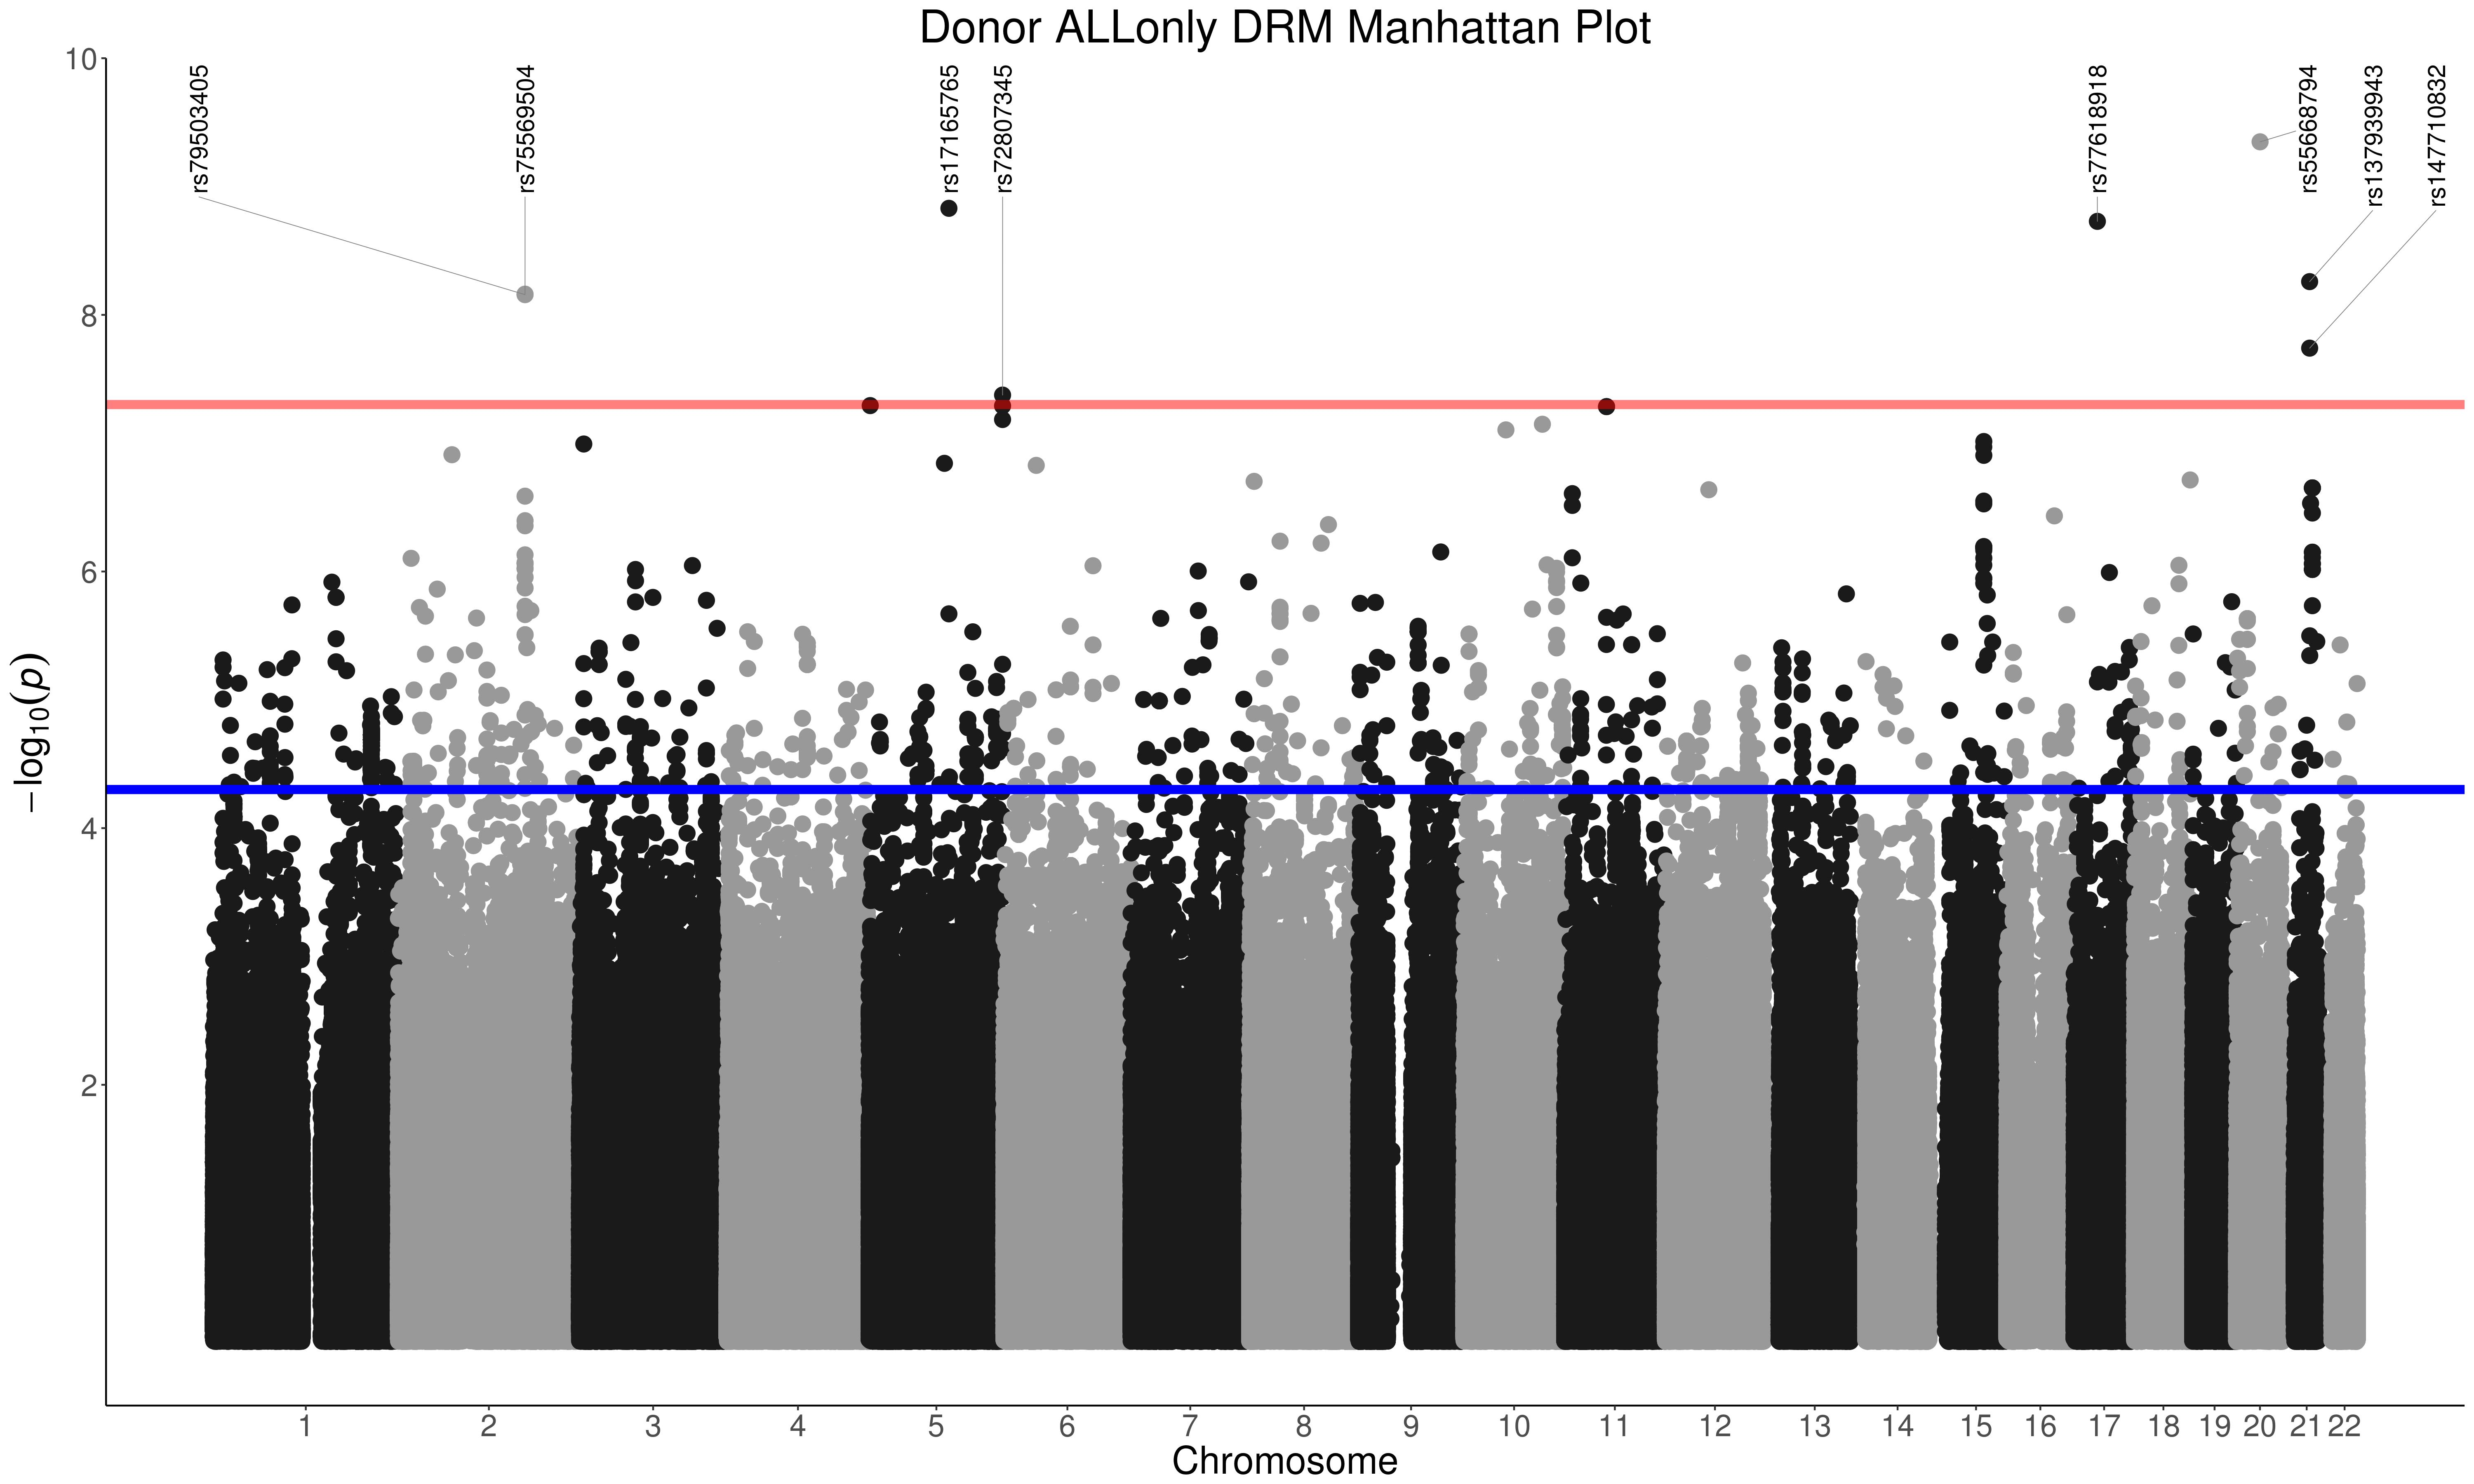
\includegraphics[width=\linewidth, height=3.5in]{~/Desktop/figures/chapter5/D_ALLonly_DRM.jpeg}
    \caption[Manhattan Plot of Donor SNPs Contribution to Recipient DRM. ]{Manhattan Plot of Donor SNPs Contribution to Recipient DRM. The x-axis is chromosome 1-22 and the y-axis is the $-\log_{10}(P_{meta})$. Each dot is a SNP. The red line is genome wide significance at $P_{meta} < 5\times{10}^{-8}$. The blue line is suggestive significance at $P_{meta} <  5\times{10}^{-5}$. Labeled SNPs are associated hits that have passed genome-wide threshold.}
    \label{fig:d_drm_1y}  
\end{figure}

\rowcolors{2}{gray!6}{white}

\begin{table}[t]

\caption{\label{tab:unnamed-chunk-40}\label{tab:d_drm_hits} DISCOVeRY-BMT Donor Genotypes Associated with Recipient Disease Related Mortality at 1-year.}
\centering
\fontsize{9}{11}\selectfont
\begin{threeparttable}
\begin{tabular}{>{\centering\arraybackslash}p{5em}|>{\centering\arraybackslash}p{5.5em}|>{\centering\arraybackslash}p{2em}|>{\centering\arraybackslash}p{10.5em}|>{\centering\arraybackslash}p{4.8em}|>{\centering\arraybackslash}p{8em}|c}
\hiderowcolors
\hline
RSID & CHR:POS & REF/ EFF & Ref. Panel/Cohort 1/ Cohort 2 MAF & P-value & HR (95\% CI) & INFO\\
\hline
\showrowcolors
rs75569504 & 2:170066550 & A/G & 0.05/0.0421/0.0272 & 6.897e-09 & 3.87 (2.45-6.12) & 0.96\\
\hline
rs79503405 & 2:170065565 & G/T & 0.0367/0.0312/0.0164 & 6.960e-09 & 5.17 (2.96-9.02) & 0.96\\
\hline
rs17165765 & 5:107206623 & C/T & 0.0111/0.0123/0.0142 & 1.478e-09 & 10.6 (4.93-22.78) & 0.83\\
\hline
rs72807345 & 5:179244672 & C/T & 0.0146/0.0173/0.0099 & 4.218e-08 & 6.04 (3.18-11.49) & 0.93\\
\hline
rs77618918 & 17:31497097 & C/T & 0.0142/0.0166/0.0059 & 1.868e-09 & 8.57 (4.25-17.27) & 0.91\\
\hline
rs55668794 & 20:31654699 & A/G & 0.0161/0.0174/0.0051 & 4.482e-10 & 9.91 (4.82-20.38) & 0.80\\
\hline
rs137939943 & 21:35231995 & G/A & 0.0097/0.0082/0.0124 & 5.509e-09 & 10.24 (4.68-22.38) & 0.86\\
\hline
rs147710832 & 21:35266776 & C/T & 0.0097/0.0091/0.0126 & 1.817e-08 & 9.66 (4.38-21.27) & 0.83\\
\hline
\end{tabular}
\begin{tablenotes}[para]
\item All SNPs shown are imputed. Genomic positions are GRCh37 reference genome. REF is reference allele and EFF is effect allele.
\end{tablenotes}
\end{threeparttable}
\end{table}

\rowcolors{2}{white}{white}

We found 5 regions associated with increased risk for DRM when donor
SNPs had the risk allele in single regions on 17, 20, and 21, and two
regions on chromosomes 2 and 5 (Figure \ref{fig:d_drm_1y};Table
\ref{tab:d_drm_hits}).

On chromsome 2, rs75569504 (Table \ref{tab:d_drm_hits}) is in strong LD
with SNPs that are intronic for \emph{MYO3B}. This marker is in perfect
LD with SNPs that bind proteins TFs Setdb1 and Hae2f1, however, little
evidence exists relating these TFs to ALL. The other region on
chromosome 2, rs79503405 was associated with increased risk in ALL DRM
and in perfect LD with an eQTL (in testes cell lines) a synonymous
variant on \emph{LRP2} (rs35114151). Synonymous mutations may affect DNA
replication processes such as transcription, splicing or translation,
any of which can have implications on phenotype.

Chromosome 5 marker rs72807345 is intronic for \emph{SQSTM1}, a gene
that has shown to be involved in somatic chromosomal abberations in
adult T-cell leukemias (Gorello et al.
\protect\hyperlink{ref-gorello_2010}{2010}). The markers are on 17 is
intronic for \emph{ASIC2} and binds proteins \emph{GR} (a highly
targetable nuclear receptor and associated with T-ALL resistance)
(McMaster and Ray \protect\hyperlink{ref-McMaster_2008}{2008}; Piovan et
al. \protect\hyperlink{ref-Piovan_2013}{2013}) and \emph{STAT3} (a well
known leukemia target gene) (Adamaki et al.
\protect\hyperlink{ref-Adamaki_2015}{2015}; Adamaki et al.
\protect\hyperlink{ref-Adamaki_2015}{2015}). When looking at the
regional association plots for the aforementioned DRM associations,
SNiPA database did not reveal any notable effects on transcriptional
regulation (Arnold et al. \protect\hyperlink{ref-snipa}{2015}).

The regions on chromosomes 20 and 21 showed no evidence of affecting
transcriptional processes from functional studies (L. D. Ward and Kellis
\protect\hyperlink{ref-haploreg}{2015}; Arnold et al.
\protect\hyperlink{ref-snipa}{2015}).

\subsection{Donor SNPs Associated with Recipient Transplant Related
Mortality}\label{donor-snps-associated-with-recipient-transplant-related-mortality}

\begin{figure}
    \centering
    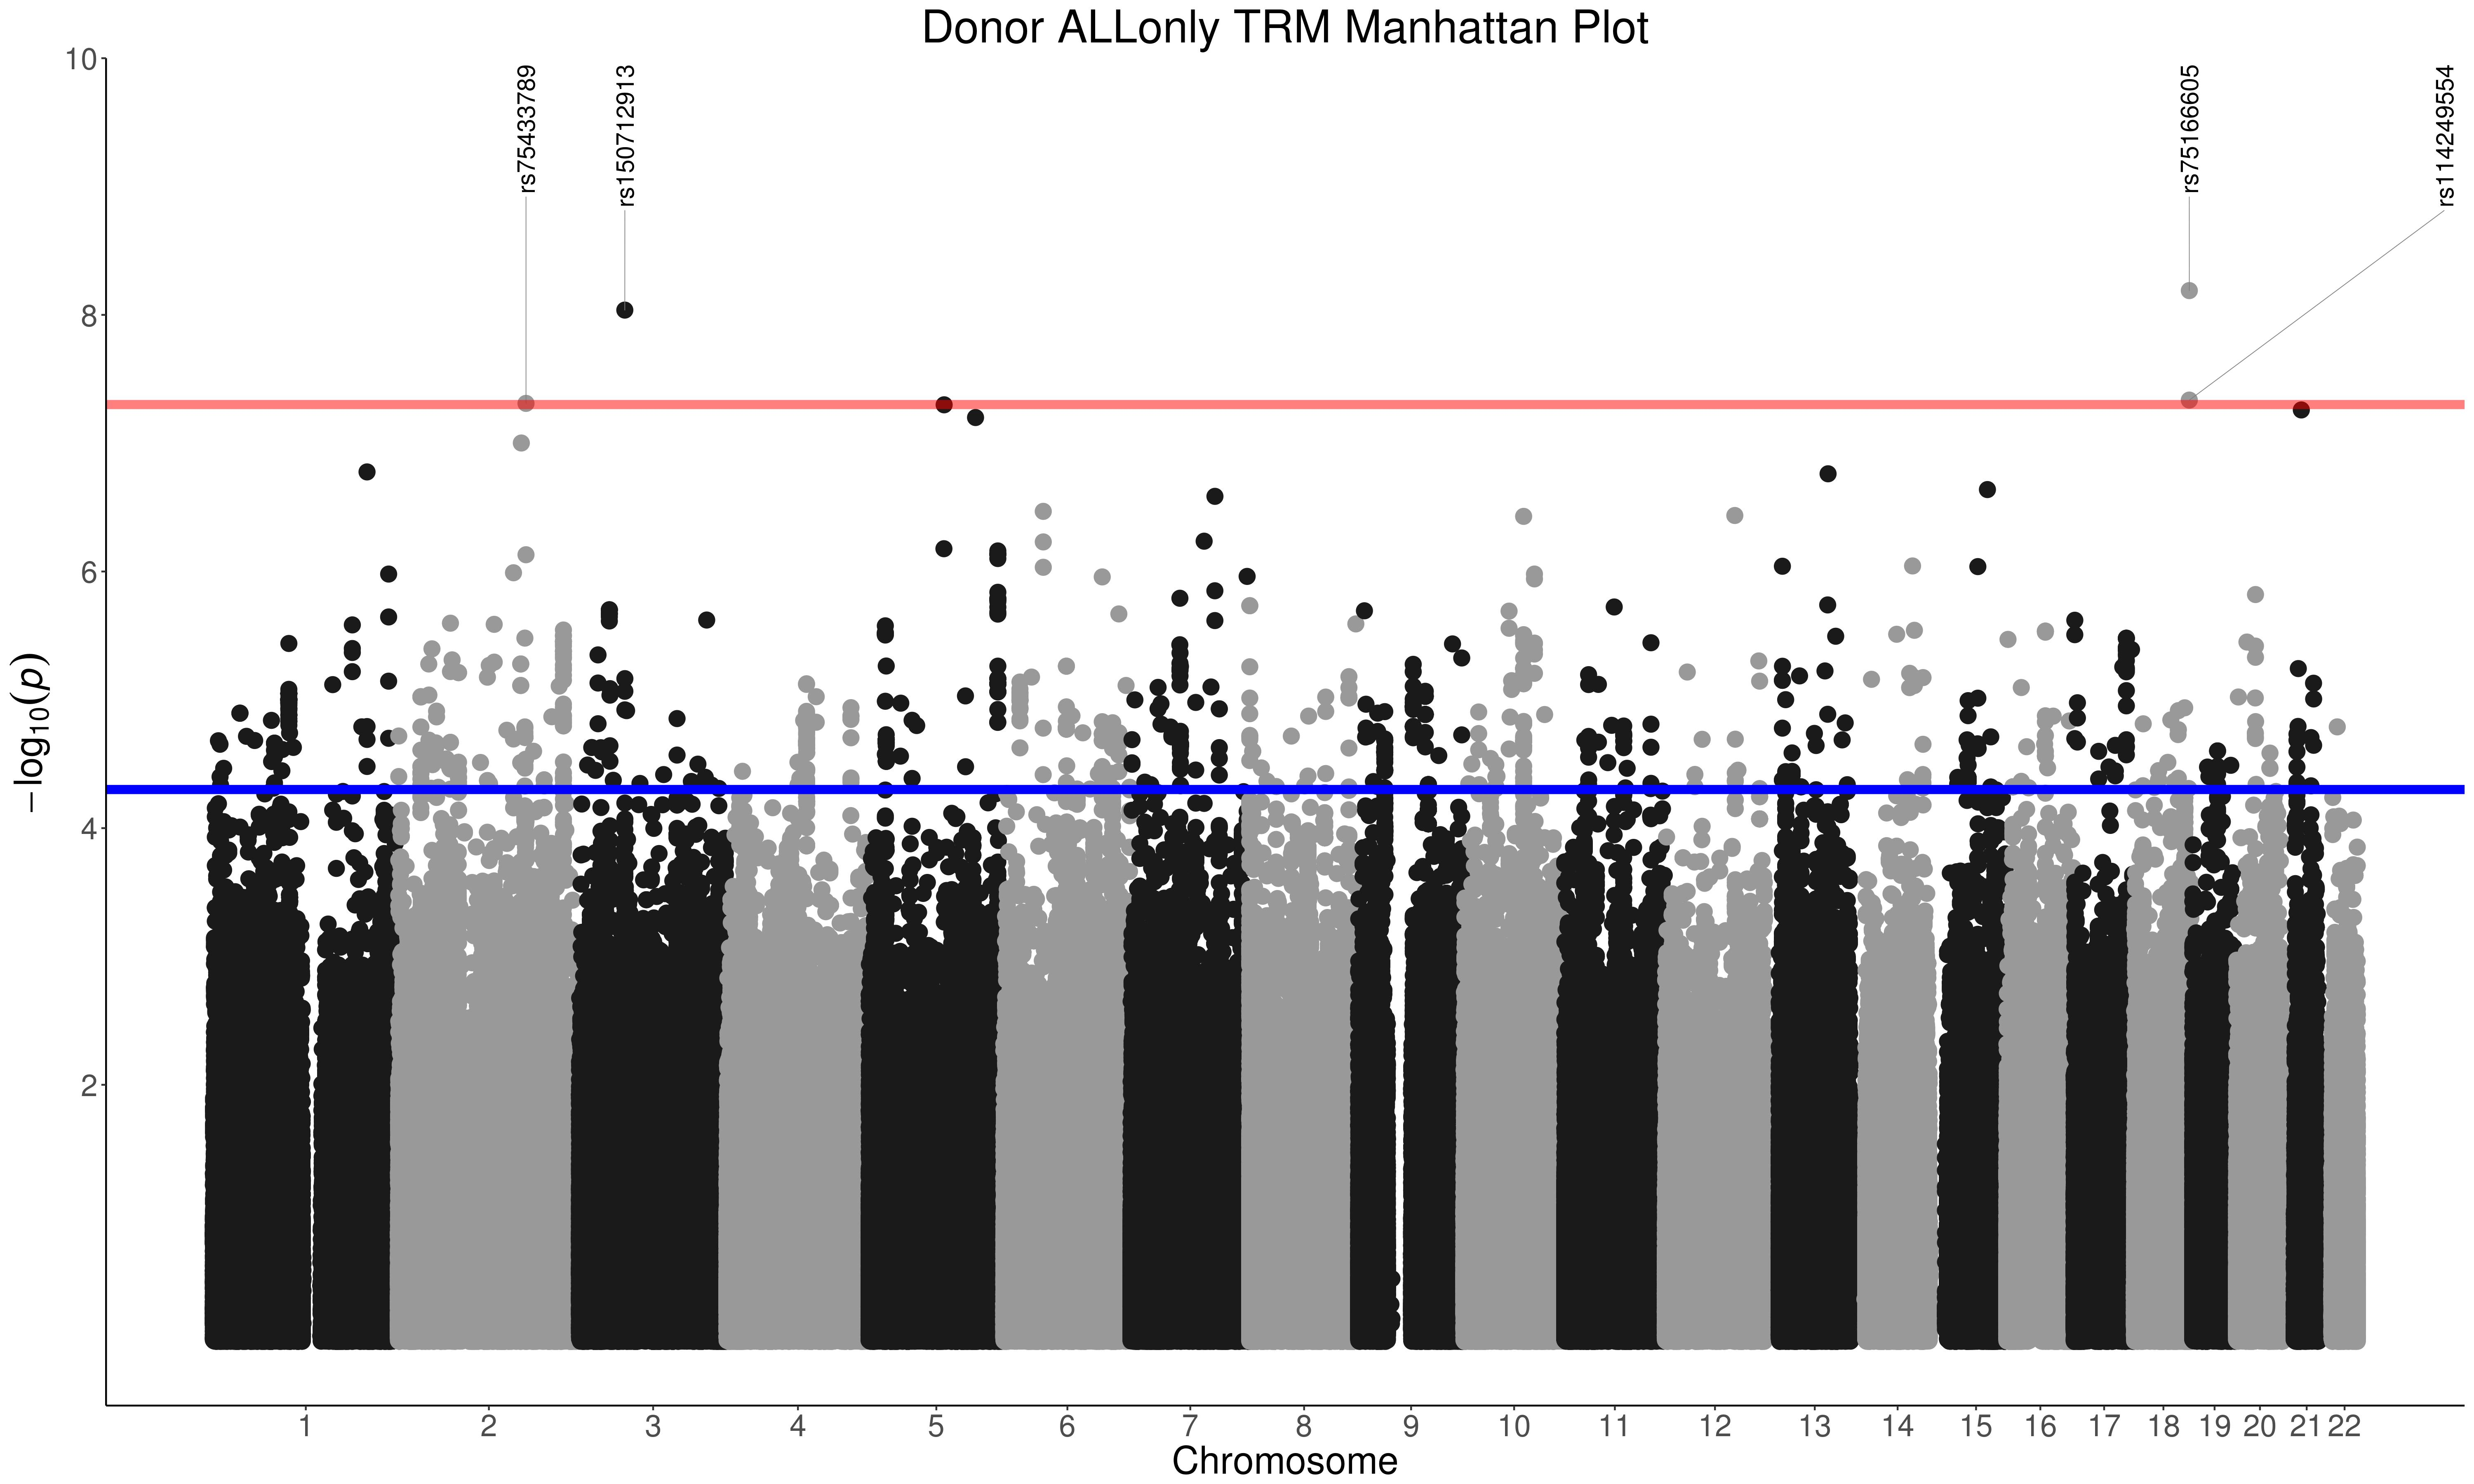
\includegraphics[width=\linewidth, height=3.5in]{~/Desktop/figures/chapter5/D_ALLonly_TRM.jpeg}
    \caption[Manhattan Plot of Donor SNPs Contribution to Recipient TRM]{Manhattan Plot of Donor SNPs Contribution to Recipient TRM. The x-axis is chromosome 1-22 and the y-axis is the $-\log_{10}(P_{meta})$. Each dot is a SNP. The red line is genome wide significance at $P_{meta} < 5\times{10}^{-8}$. The blue line is suggestive significance at $P_{meta} <  5\times{10}^{-5}$. Labeled SNPs are associated hits that have passed genome-wide threshold.}
    \label{fig:d_trm_1y}  
\end{figure}

\rowcolors{2}{gray!6}{white}

\begin{table}[t]

\caption{\label{tab:unnamed-chunk-41}\label{tab:r_os_hits} DISCOVeRY-BMT Donor Genotypes Associated with Recipent Transplant Related Mortality at 1-year.}
\centering
\fontsize{9}{11}\selectfont
\begin{threeparttable}
\begin{tabular}{>{\centering\arraybackslash}p{5em}|>{\centering\arraybackslash}p{5.5em}|>{\centering\arraybackslash}p{2em}|>{\centering\arraybackslash}p{10.5em}|>{\centering\arraybackslash}p{4.8em}|>{\centering\arraybackslash}p{8em}|c}
\hiderowcolors
\hline
RSID & CHR:POS & REF/ EFF & Ref. Panel/Cohort 1/ Cohort 2 MAF & P-value & HR (95\% CI) & INFO\\
\hline
\showrowcolors
rs75433789 & 2:171353397 & C/T & 0.0096/0.0059/0.0054 & 4.897e-08 & 12.31 (4.99-30.33) & 0.92\\
\hline
rs150712913 & 3:60957357 & G/C & 0.0137/0.0122/0.0167 & 9.181e-09 & 8.12 (3.97-16.58) & 0.84\\
\hline
rs117595188 & 15:63517319 & G/T & 0.0078/0.0107/0.0129 & 2.376e-08 & 7.99 (3.85-16.56) & 0.85\\
\hline
rs75166605 & 18:73806958 & G/A & 0.0067/0.0065/0.0199 & 6.470e-09 & 13.03 (5.48-31.01) & 0.96\\
\hline
rs114249554 & 18:73779508 & T/G & 0.006/0.0059/0.0161 & 4.615e-08 & 13.66 (5.35-34.87) & 0.93\\
\hline
\end{tabular}
\begin{tablenotes}[para]
\item All SNPs shown are imputed. Genomic positions are GRCh37 reference genome. REF is reference allele and EFF is effect allele.
\end{tablenotes}
\end{threeparttable}
\end{table}

\rowcolors{2}{white}{white}

Our analyses revealed TRM associations with donor SNPs on chromosomes 2,
3, 15, 18 and 20 (Table \ref{tab:r_os_hits}; Figure \ref{fig:d_trm_1y}).
The associated SNPs in chromosome 2 are in LD and are located in the
intronic region of \emph{MYO3B} gene (L. D. Ward and Kellis
\protect\hyperlink{ref-haploreg}{2015}). The chromosome 2 associations
are driven by disease death, as we also observed significant SNPs in
this region for DRM. Although lack of \emph{FHIT} at the protein level
has been shown to induce leukemia (U. R. Peters et al.
\protect\hyperlink{ref-peters_1999}{1999}), the associated intronic SNP
on chromosome 3 had minimal evidence of transcriptional regulation from
existing literature based on experimental evidence (Arnold et al.
\protect\hyperlink{ref-snipa}{2015}). Similarly, the associated
chromosome 18 region for donor SNPs showed effect on transcription (L.
D. Ward and Kellis \protect\hyperlink{ref-haploreg}{2015}; Arnold et al.
\protect\hyperlink{ref-snipa}{2015}).

\subsection{Donor SNPs Associated with Graft-versus-Host
Disease}\label{donor-snps-associated-with-graft-versus-host-disease}

\begin{figure}
    \centering
    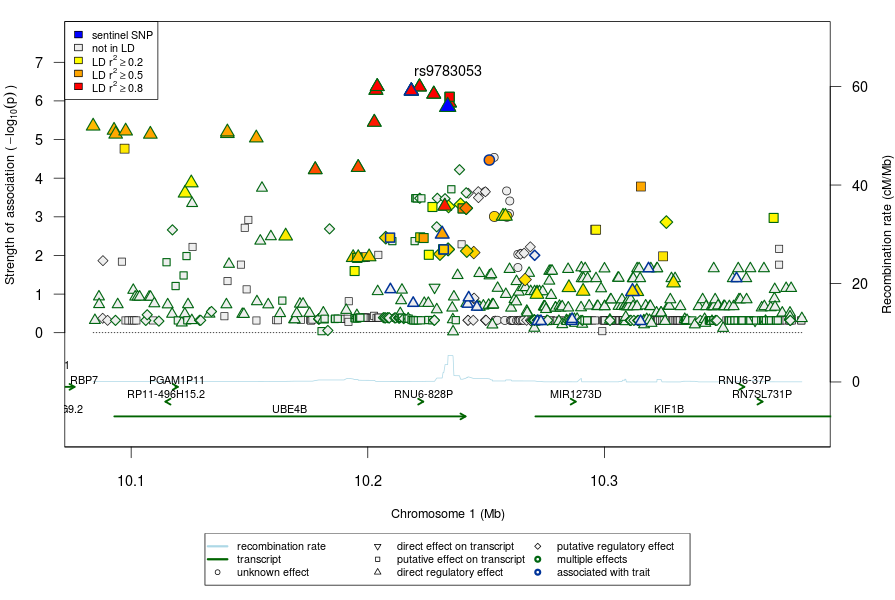
\includegraphics[width=\linewidth, height=3.5in]{~/Desktop/figures/chapter5/rs9783053_1_D_ALLonly_GVHD.png}
    \caption[Donor GVHD Region Chromosome 1.]{Donor GVHD Region Chromosome 1. Sentinel SNP is rs9783053 and colored blue. The region comprises +/- 150 kb window from the sentinel SNP. The red-yellow color gradient represents LD strength. Shapes represent different effects that the SNP has been reported to have in this region from independent studies.}
    \label{fig:d_gvhd_1y}  
\end{figure}

We scanned suggestive SNP regions (\(P < 5\times{10}^{-5}\)) for regions
that may affect transcription factor binding. Donor GVHD SNP rs9783053
(typed SNP; \(P=1.41\times{10}^{-6}\); HR: 3.27 {[}2.02-5.29{]}; G
effect allele) was found to have a regulomeDB score of 1A (the highest
score). This means based off of previous literature, there is strong
evidence that rs9783053 affects transcription factor binding (Boyle et
al. \protect\hyperlink{ref-Boyle_2012}{2012}). This region has many SNPs
that directly regulate transcription on \emph{UBE4B} (Figure
\ref{fig:d_gvhd_1y}). This polymorphism has five proteins (Ctcf, Ebf1,
Elf1, Nf\(\kappa\)b, Pu1) that bind to this SNP in lymphoblastoid cell
lines (ENCODE Project Consortium
\protect\hyperlink{ref-encode_2012}{2012}). This variant is in LD with
synonymous variant rs2273299 (\(r^2=0.88\)). Experimental cell line
studies from ENCODE provide evidence suggesting that this region alters
regulatory motifs for cancer and leukemia related genes (L. D. Ward and
Kellis \protect\hyperlink{ref-haploreg}{2015}). Variants that alter gene
expression were found in blood and lymphoblast derived CEU cell lines.
Thus, while donor GVHD SNPs did not reach genome-wide significance, the
is some evidence that suggests this region may transcriptional or
epigenetic on effects on ALL related genes.

\section{Discussion}\label{discussion-4}

Previously the relationship between survival outcomes and non-HLA
donor-recipient genetics after MUD-HSCT had not been studied at the
genome-wide level. Here we presented the first GWAS investigating this
objective. The cohorts of DISCOVeRY-BMT span the entire ALL patient
pool, ranging from childhood, AYA, adults and senior adults. Genome-wide
associations to survival outcomes after 1-year post-transplant were
identified in both recipient and donor genomes. Specifically, recipient
DRM, OS, and OF. And for donors, associations were found for DRM, TRM,
GVHD, and OS. Often our genome-wide associations provided only a small
insights of possible biological mechanisms that may contribute to these
observed death related phenotypes.

We attempted to gain additional insight by leveraging publicly available
databases. We inspected regions that were below genome-wide significance
at \(P < 5\times{10}^{-5}\). Often we found regions that were in fact
not genome-wide significant, but regional association plots revealed
that there may some effect on transcription and that previous studies
have provided evidence that these regions have many interactions. Future
directions for this project include implementing PrediXcan which is
currently underway in the lab and will be added to this work before
publication. PrediXcan always assessment of gene-based expression levels
in our data and thus will help us prioritize our GWAS associations.
Future directions for this project include implementing PrediXcan
(Barbeira et al. \protect\hyperlink{ref-Barbeira_2018}{2018}) which is
currently underway in the lab and will be added to this work before
publication. PrediXcan allows assessment of gene-based expression levels
in our data (using blood tissue samples from GTEx) and thus will help us
prioritize our GWAS associations.

Although DISCOVeRY-BMT is the largest cohort to date investigating ALL
recipient-donor genetic variation after transplant, sample size remains
a large limitation. The next step will be replicate these findings in an
independent study. Namely using University of Washington ALL cohort
study for replication of relapse and overall survival. If available, in
addition to replication using University of Washington cohorts,
meta-analysis combining DISCOVeRY-BMT may provide stronger signal for
overall survival and/or relapse outcomes. In terms of improving our
survival models, alterations to our current workflow may improve signal
by adjusting for age by stratifying by clinical age groups, or by
modeling the age as a non-linear function and smoothing the distribution
using splines (Shepherd, Rebeiro, and Caribbean, Central and South
America network for HIV epidemiology
\protect\hyperlink{ref-shepherd_2017}{2017}). Challenges in improving
long-term survival after MUD-HSCT remain, however, we believe that this
study provides unique insights in this field and is a positive step
towards improving outcomes.

\FloatBarrier

\newpage

\pagestyle{plain} \fancyhead[L]{} \fancyhead[R]{}
\fancyfoot[C]{\thepage}

\chapter{Conclusion and Future Work}

\doublespacing

Modern science progresses through corroboration, computing, and
collaboration. \emph{Corroboration} by the need to continually seek
answers and verify results. Reproducibility is necessary for robust
ideas and expansion of knowledge. In genomics, traditional biomedical
researchers often study one gene for one phenotype for numerous years,
possibly decades. More often than not, these hypotheses propagate from a
single study years ago or from using \emph{a priori} information of a
specific system in hypothesis development. Unfortunately, often, the
original studies were never reproduced in well-designed independent
studies. Constant pursuit of false leads may impede the rate at which
important problems are solved. Agnostic approaches through usage of
genome-wide technologies (such as GWAS), allow researchers to inspect
phenotypes and gain biological insights at a global level. As technology
continues to advance, data collection and data resources inherently
grow. Multiple rich data resources are available from all aspects of the
genome, the \emph{-omics} (i.e.~genomics, transcriptomics, metabolomics,
proteomics, methylation), as well as clinical trials. As such, large
scale \emph{computing} is imperative to the success of modern studies.
Broader insights can be leveraged to develop hypotheses that can
investigate and characterize complex disease etyiology. And the last
element in order to accomplsih anything is \emph{collaboration} by
conducting team science. Bringing together multiple talented individuals
and groups together and enriching each other with combined expertise to
achieve a common goal.

This dissertation was an attempt to exemplify these principles of modern
science to the best of our ability. I was very fortunate to join a lab
that had an incredibly rich clinically relevant data source, the
DISCOVeRY-BMT GWAS. DISCOVeRY-BMT is a fine example of collaborative
team science. The team is made up of scientists, clincians, and
statisticians (and some who belong to more than one of those groups)
from multiple institutions. With this GWAS, we attempted to corroborate
researchers that continually pursued candidate SNPs in candidate genes
that they believed held some biological relevance to survival in
recipients or donors after transplant. We were unable to reproduce any
of their results using DISCOVeRY BMT's much larger and more homogeneous
study population. While we published on a negative result, we were able
to make an important contribution to the transplant field by providing
strong evidence that those studies should begin looking elsewhere in the
genome for hidden insights.

We were able to address a computational challenges in genomics,
specifically when it comes to survival analysis. We developed an
R/Bioconductor package, gwasurvivr, that can directly take data from
online imputation web services. As large studies continue to get funded
with well-documented follow up data -- survival studies will continue to
become more prevalent. Gwasurvivr will be an important computational
resource for the next several years. To date, over 200 unique IPs have
downloaded gwasurvivr. We were also able to develop a pipeline that
enhanced our workflow and reproducibility efforts. The pipeline should
be expanded to automate annotation using SNiPA database and HaploReg.
Construction of a centralized database (PostgreSQL database) is underway
that will continue to enhance our workflow.

We were able to use our own software and pipeline to perform many GWAS
using DISCOVeRY-BMT. While we reported recipient and donor SNP
associations to survival outcomes post-HSCT, there remains the entire
DISCOVeRY-BMT 100 day censoring analyses for ALL (and our other disesase
groups). These results have yet to be analyzed, curated, and reported.
These results are very important and relevant to the transplant field as
patients that die within the first 100 days may present very different
genetic profiles than those who survive until at least 1 year. This
research will continue after my departure from our lab and I believe it
will be quite impactful.

\FloatBarrier

\newpage

\pagestyle{plain} \fancyhead[L]{} \fancyhead[R]{}
\fancyfoot[C]{\thepage}

\chapter*{REFERENCES}

\singlespacing
\setlength{\parindent}{-0.5in} \setlength{\leftskip}{0.4in}
\setlength{\parskip}{12pt}

\hypertarget{refs}{}
\hypertarget{ref-1000genomes}{}
1000 Genomes Project Consortium. 2015. ``A Global Reference for Human
Genetic Variation.'' \emph{Nature} 526 (7571). Nature Publishing Group:
68.

\hypertarget{ref-1kb_phase1}{}
1000 Genomes Project Consortium, Gonçalo R Abecasis, David Altshuler,
Adam Auton, Lisa D Brooks, Richard M Durbin, Richard A Gibbs, Matt E
Hurles, and Gil A McVean. 2010. ``A Map of Human Genome Variation from
Population-Scale Sequencing.'' \emph{Nature} 467 (7319): 1061--73.
doi:\href{https://doi.org/10.1038/nature09534}{10.1038/nature09534}.

\hypertarget{ref-Adamaki_2015}{}
Adamaki, Maria, Maria Tsotra, Spiros Vlahopoulos, Archontis
Zampogiannis, Athanasios G Papavassiliou, and Maria Moschovi. 2015.
``STAT Transcript Levels in Childhood Acute Lymphoblastic Leukemia:
STAT1 and Stat3 Transcript Correlations.'' \emph{Leuk Res}, September.
doi:\href{https://doi.org/10.1016/j.leukres.2015.09.004}{10.1016/j.leukres.2015.09.004}.

\hypertarget{ref-Akasaka_2007}{}
Akasaka, Takashi, Theodore Balasas, Lisa J Russell, Kei-ji Sugimoto,
Aneela Majid, Renata Walewska, E Loraine Karran, et al. 2007. ``Five
Members of the Cebp Transcription Factor Family Are Targeted by
Recurrent Igh Translocations in B-Cell Precursor Acute Lymphoblastic
Leukemia (Bcp-All).'' \emph{Blood} 109 (8): 3451--61.
doi:\href{https://doi.org/10.1182/blood-2006-08-041012}{10.1182/blood-2006-08-041012}.

\hypertarget{ref-snipa}{}
Arnold, Matthias, Johannes Raffler, Arne Pfeufer, Karsten Suhre, and
Gabi Kastenmüller. 2015. ``SNiPA: An Interactive, Genetic
Variant-Centered Annotation Browser.'' \emph{Bioinformatics} 31 (8):
1334--6.
doi:\href{https://doi.org/10.1093/bioinformatics/btu779}{10.1093/bioinformatics/btu779}.

\hypertarget{ref-bolanos_2016}{}
Arrieta-Bolaños, Esteban, Neema P Mayor, Steven G E Marsh, J Alejandro
Madrigal, Jane F Apperley, Keiren Kirkland, Stephen Mackinnon, et al.
2016. ``Polymorphism in Tgfb1 Is Associated with Worse Non-Relapse
Mortality and Overall Survival After Stem Cell Transplantation with
Unrelated Donors.'' \emph{Haematologica} 101 (3): 382--90.
doi:\href{https://doi.org/10.3324/haematol.2015.134999}{10.3324/haematol.2015.134999}.

\hypertarget{ref-bakker_2008}{}
Bakker, Paul I W de, Manuel A R Ferreira, Xiaoming Jia, Benjamin M
Neale, Soumya Raychaudhuri, and Benjamin F Voight. 2008. ``Practical
Aspects of Imputation-Driven Meta-Analysis of Genome-Wide Association
Studies.'' \emph{Hum Mol Genet} 17 (R2): R122--8.
doi:\href{https://doi.org/10.1093/hmg/ddn288}{10.1093/hmg/ddn288}.

\hypertarget{ref-bakker_2005}{}
Bakker, Paul I W de, Roman Yelensky, Itsik Pe'er, Stacey B Gabriel, Mark
J Daly, and David Altshuler. 2005. ``Efficiency and Power in Genetic
Association Studies.'' \emph{Nat Genet} 37 (11): 1217--23.
doi:\href{https://doi.org/10.1038/ng1669}{10.1038/ng1669}.

\hypertarget{ref-balavarca_2015}{}
Balavarca, Y, K Pearce, J Norden, M Collin, G Jackson, E Holler, R
Dressel, et al. 2015. ``Predicting Survival Using Clinical Risk Scores
and Non-Hla Immunogenetics.'' \emph{Bone Marrow Transplant} 50 (11):
1445--52.
doi:\href{https://doi.org/10.1038/bmt.2015.173}{10.1038/bmt.2015.173}.

\hypertarget{ref-Barbeira_2018}{}
Barbeira, Alvaro N, Scott P Dickinson, Rodrigo Bonazzola, Jiamao Zheng,
Heather E Wheeler, Jason M Torres, Eric S Torstenson, et al. 2018.
``Exploring the Phenotypic Consequences of Tissue Specific Gene
Expression Variation Inferred from Gwas Summary Statistics.''
\emph{Nature Communications} 9 (1): 1825.
doi:\href{https://doi.org/10.1038/s41467-018-03621-1}{10.1038/s41467-018-03621-1}.

\hypertarget{ref-Boyle_2012}{}
Boyle, Alan P, Eurie L Hong, Manoj Hariharan, Yong Cheng, Marc A Schaub,
Maya Kasowski, Konrad J Karczewski, et al. 2012. ``Annotation of
Functional Variation in Personal Genomes Using Regulomedb.''
\emph{Genome Research} 22 (9): 1790--7.
doi:\href{https://doi.org/10.1101/gr.137323.112}{10.1101/gr.137323.112}.

\hypertarget{ref-breslow1974}{}
Breslow, Norman. 1974. ``Covariance Analysis of Censored Survival
Data.'' \emph{Biometrics}. JSTOR, 89--99.

\hypertarget{ref-browning_2016}{}
Browning, Brian L, and Sharon R Browning. 2016. ``Genotype Imputation
with Millions of Reference Samples.'' \emph{Am J Hum Genet} 98 (1):
116--26.
doi:\href{https://doi.org/10.1016/j.ajhg.2015.11.020}{10.1016/j.ajhg.2015.11.020}.

\hypertarget{ref-cavet_2001}{}
Cavet, J, A M Dickinson, J Norden, P R Taylor, G H Jackson, and P G
Middleton. 2001. ``Interferon-Gamma and Interleukin-6 Gene Polymorphisms
Associate with Graft-Versus-Host Disease in Hla-Matched Sibling Bone
Marrow Transplantation.'' \emph{Blood} 98 (5): 1594--1600.

\hypertarget{ref-chang_2009}{}
Chang, Ya-Yi, Hildegard T Greinix, Anne M Dickinson, Daniel Wolff,
Graham H Jackson, Reinhard Andreesen, Ernst Holler, and Gerhard C
Hildebrandt. 2009. ``G to c Transition at Position -173 of Mif Gene of
the Recipient Is Associated with Reduced Relapse Rates After Allogeneic
Stem Cell Transplantation.'' \emph{Cytokine} 48 (3): 218--25.
doi:\href{https://doi.org/10.1016/j.cyto.2009.07.012}{10.1016/j.cyto.2009.07.012}.

\hypertarget{ref-chien_2012}{}
Chien, Jason W, Xinyi Cindy Zhang, Wenhong Fan, Hongwei Wang, Lue Ping
Zhao, Paul J Martin, Barry E Storer, Michael Boeckh, Edus H Warren, and
John A Hansen. 2012. ``Evaluation of Published Single Nucleotide
Polymorphisms Associated with Acute Gvhd.'' \emph{Blood} 119 (22):
5311--9.
doi:\href{https://doi.org/10.1182/blood-2011-09-371153}{10.1182/blood-2011-09-371153}.

\hypertarget{ref-Clay_2017}{}
Clay-Gilmour, Alyssa I., Theresa Hahn, Leah M. Preus, Kenan Onel, Andrew
Skol, Eric Hungate, Qianqian Zhu, et al. 2017. ``Genetic Association
with B-Cell Acute Lymphoblastic Leukemia in Allogeneic Transplant
Patients Differs by Age and Sex.'' \emph{Blood Advances} 1 (20):
1717--28.

\hypertarget{ref-motifbreakr}{}
Coetzee, Simon G., Gerhard A. Coetzee, and Dennis J. Hazelett. 2015.
``MotifbreakR: An R/Bioconductor Package for Predicting Variant Effects
at Transcription Factor Binding Sites.'' \emph{Bioinformatics}.
doi:\href{https://doi.org/10.1093/bioinformatics/btv470}{10.1093/bioinformatics/btv470}.

\hypertarget{ref-colhoun2003}{}
Colhoun, Helen M, Paul M McKeigue, and George Davey Smith. 2003.
``Problems of Reporting Genetic Associations with Complex Outcomes.''
\emph{The Lancet} 361 (9360). Elsevier: 865--72.

\hypertarget{ref-copelan_2006}{}
Copelan, Edward A. 2006. ``Hematopoietic Stem-Cell Transplantation.''
\emph{N Engl J Med} 354 (17): 1813--26.
doi:\href{https://doi.org/10.1056/NEJMra052638}{10.1056/NEJMra052638}.

\hypertarget{ref-cox1972}{}
Cox, David R. 1972. ``Regression Models and Life-Tables.'' \emph{Journal
of the Royal Statistical Society: Series B (Methodological)} 34 (2).
Wiley Online Library: 187--202.

\hypertarget{ref-michigan_imputation}{}
Das, Sayantan, Lukas Forer, Sebastian Schönherr, Carlo Sidore, Adam E
Locke, Alan Kwong, Scott I Vrieze, et al. 2016. ``Next-Generation
Genotype Imputation Service and Methods.'' \emph{Nature Genetics} 48
(10). Nature Publishing Group: 1284.

\hypertarget{ref-shapeit2}{}
Delaneau, Olivier, Bryan Howie, Anthony J Cox, Jean-François Zagury, and
Jonathan Marchini. 2013. ``Haplotype Estimation Using Sequencing
Reads.'' \emph{Am J Hum Genet} 93 (4): 687--96.
doi:\href{https://doi.org/10.1016/j.ajhg.2013.09.002}{10.1016/j.ajhg.2013.09.002}.

\hypertarget{ref-durbin_2014}{}
Durbin, Richard. 2014. ``Efficient Haplotype Matching and Storage Using
the Positional Burrows-Wheeler Transform (Pbwt).'' \emph{Bioinformatics}
30 (9): 1266--72.
doi:\href{https://doi.org/10.1093/bioinformatics/btu014}{10.1093/bioinformatics/btu014}.

\hypertarget{ref-DSouza_2017}{}
D'Souza, Anita, Stephanie Lee, Xiaochun Zhu, and Marcelo Pasquini. 2017.
``Current Use and Trends in Hematopoietic Cell Transplantation in the
United States.'' \emph{Biology of Blood and Marrow Transplantation} 23
(9): 1417--21.
doi:\href{https://doi.org/10.1016/j.bbmt.2017.05.035}{10.1016/j.bbmt.2017.05.035}.

\hypertarget{ref-efron1977}{}
Efron, Bradley. 1977. ``The Efficiency of Cox's Likelihood Function for
Censored Data.'' \emph{Journal of the American Statistical Association}
72 (359). Taylor \& Francis: 557--65.

\hypertarget{ref-encode_2012}{}
ENCODE Project Consortium. 2012. ``An Integrated Encyclopedia of Dna
Elements in the Human Genome.'' \emph{Nature} 489 (7414): 57--74.
doi:\href{https://doi.org/10.1038/nature11247}{10.1038/nature11247}.

\hypertarget{ref-Fehrmann_2011}{}
Fehrmann, Rudolf S N, Ritsert C Jansen, Jan H Veldink, Harm-Jan Westra,
Danny Arends, Marc Jan Bonder, Jingyuan Fu, et al. 2011. ``Trans-eQTLs
Reveal That Independent Genetic Variants Associated with a Complex
Phenotype Converge on Intermediate Genes, with a Major Role for the
Hla.'' \emph{PLoS Genetics} 7 (8): e1002197.
doi:\href{https://doi.org/10.1371/journal.pgen.1002197}{10.1371/journal.pgen.1002197}.

\hypertarget{ref-fine1999}{}
Fine, Jason P, and Robert J Gray. 1999. ``A Proportional Hazards Model
for the Subdistribution of a Competing Risk.'' \emph{Journal of the
American Statistical Association} 94 (446). Taylor \& Francis: 496--509.

\hypertarget{ref-gallagher_2018}{}
Gallagher, Michael D, and Alice S Chen-Plotkin. 2018. ``The Post-Gwas
Era: From Association to Function.'' \emph{Am J Hum Genet} 102 (5):
717--30.
doi:\href{https://doi.org/10.1016/j.ajhg.2018.04.002}{10.1016/j.ajhg.2018.04.002}.

\hypertarget{ref-gwastools}{}
Gogarten, Stephanie M, Tushar Bhangale, Matthew P Conomos, Cecelia A
Laurie, Caitlin P McHugh, Ian Painter, Xiuwen Zheng, et al. 2012.
``GWASTools: An R/Bioconductor Package for Quality Control and Analysis
of Genome-Wide Association Studies.'' \emph{Bioinformatics} 28 (24).
Oxford University Press: 3329--31.

\hypertarget{ref-gorello_2010}{}
Gorello, Paolo, Roberta La Starza, Danika Di Giacomo, Monica Messina,
Maria Cristina Puzzolo, Barbara Crescenzi, Alessandra Santoro, Sabina
Chiaretti, and Cristina Mecucci. 2010. ``SQSTM1-Nup214: A New Gene
Fusion in Adult T-Cell Acute Lymphoblastic Leukemia.''
\emph{Haematologica} 95 (12): 2161--3.
doi:\href{https://doi.org/10.3324/haematol.2010.029769}{10.3324/haematol.2010.029769}.

\hypertarget{ref-grambsch_ph}{}
Grambsch, Patricia M, and Terry M Therneau. 1994. ``Proportional Hazards
Tests and Diagnostics Based on Weighted Residuals.'' \emph{Biometrika}
81 (3). Oxford University Press: 515--26.

\hypertarget{ref-green_2003}{}
Green, Richard E, Benjamin P Lewis, R Tyler Hillman, Marco Blanchette,
Liana F Lareau, Aaron T Garnett, Donald C Rio, and Steven E Brenner.
2003. ``Widespread Predicted Nonsense-Mediated mRNA Decay of
Alternatively-Spliced Transcripts of Human Normal and Disease Genes.''
\emph{Bioinformatics} 19 Suppl 1: i118--21.

\hypertarget{ref-gtex}{}
GTEx Consortium. 2013. ``The Genotype-Tissue Expression (Gtex)
Project.'' \emph{Nat Genet} 45 (6): 580--5.
doi:\href{https://doi.org/10.1038/ng.2653}{10.1038/ng.2653}.

\hypertarget{ref-Guerzoni_2006}{}
Guerzoni, Clara, Michela Bardini, Samanta A Mariani, Giovanna
Ferrari-Amorotti, Paolo Neviani, Maria Luisa Panno, Ying Zhang, Robert
Martinez, Danilo Perrotti, and Bruno Calabretta. 2006. ``Inducible
Activation of Cebpb, a Gene Negatively Regulated by Bcr/Abl, Inhibits
Proliferation and Promotes Differentiation of Bcr/Abl-Expressing
Cells.'' \emph{Blood} 107 (10): 4080--9.
doi:\href{https://doi.org/10.1182/blood-2005-08-3181}{10.1182/blood-2005-08-3181}.

\hypertarget{ref-Hahn_2015}{}
Hahn, Theresa, Lara E Sucheston-Campbell, Leah Preus, Xiaochun Zhu, John
A Hansen, Paul J Martin, Li Yan, et al. 2015. ``Establishment of
Definitions and Review Process for Consistent Adjudication of
Cause-Specific Mortality After Allogeneic Unrelated-Donor Hematopoietic
Cell Transplantation.'' \emph{Biology of Blood and Marrow
Transplantation} 21 (9): 1679--86.
doi:\href{https://doi.org/10.1016/j.bbmt.2015.05.019}{10.1016/j.bbmt.2015.05.019}.

\hypertarget{ref-hamilton_2012}{}
Hamilton, Betty K, and Edward A Copelan. 2012. ``Concise Review: The
Role of Hematopoietic Stem Cell Transplantation in the Treatment of
Acute Myeloid Leukemia.'' \emph{Stem Cells} 30 (8): 1581--6.
doi:\href{https://doi.org/10.1002/stem.1140}{10.1002/stem.1140}.

\hypertarget{ref-Henig_2014}{}
Henig, Israel, and Tsila Zuckerman. 2014. ``Hematopoietic Stem Cell
Transplantation-50 Years of Evolution and Future Perspectives.''
\emph{Rambam Maimonides Medical Journal} 5 (4): e0028.
doi:\href{https://doi.org/10.5041/RMMJ.10162}{10.5041/RMMJ.10162}.

\hypertarget{ref-holler_2008}{}
Holler, E, G Rogler, J Brenmoehl, J Hahn, H Greinix, A M Dickinson, G
Socie, et al. 2008. ``The Role of Genetic Variants of Nod2/Card15, a
Receptor of the Innate Immune System, in Gvhd and Complications
Following Related and Unrelated Donor Haematopoietic Stem Cell
Transplantation.'' \emph{Int J Immunogenet} 35 (4-5): 381--4.
doi:\href{https://doi.org/10.1111/j.1744-313X.2008.00795.x}{10.1111/j.1744-313X.2008.00795.x}.

\hypertarget{ref-holler_2004}{}
Holler, Ernst, Gerhard Rogler, Hans Herfarth, Julia Brenmoehl, Peter
Johannes Wild, Joachim Hahn, Günther Eissner, Jürgen Schölmerich, and
Reinhard Andreesen. 2004. ``Both Donor and Recipient Nod2/Card15
Mutations Associate with Transplant-Related Mortality and Gvhd Following
Allogeneic Stem Cell Transplantation.'' \emph{Blood} 104 (3): 889--94.
doi:\href{https://doi.org/10.1182/blood-2003-10-3543}{10.1182/blood-2003-10-3543}.

\hypertarget{ref-Howie_2009}{}
Howie, Bryan N, Peter Donnelly, and Jonathan Marchini. 2009. ``A
Flexible and Accurate Genotype Imputation Method for the Next Generation
of Genome-Wide Association Studies.'' \emph{PLoS Genetics} 5 (6):
e1000529.
doi:\href{https://doi.org/10.1371/journal.pgen.1000529}{10.1371/journal.pgen.1000529}.

\hypertarget{ref-hu_2006}{}
Hu, Hui, Bin Wang, Madhuri Borde, Julie Nardone, Shan Maika, Laura
Allred, Philip W Tucker, and Anjana Rao. 2006. ``Foxp1 Is an Essential
Transcriptional Regulator of B Cell Development.'' \emph{Nat Immunol} 7
(8): 819--26. doi:\href{https://doi.org/10.1038/ni1358}{10.1038/ni1358}.

\hypertarget{ref-Huguet_2009}{}
Huguet, Françoise, Thibaut Leguay, Emmanuel Raffoux, Xavier Thomas,
Kheira Beldjord, Eric Delabesse, Patrice Chevallier, et al. 2009.
``Pediatric-Inspired Therapy in Adults with Philadelphia
Chromosome-Negative Acute Lymphoblastic Leukemia: The Graall-2003
Study.'' \emph{J Clin Oncol} 27 (6): 911--8.
doi:\href{https://doi.org/10.1200/JCO.2008.18.6916}{10.1200/JCO.2008.18.6916}.

\hypertarget{ref-Iacobucci_2017}{}
Iacobucci, Ilaria, and Charles G Mullighan. 2017. ``Genetic Basis of
Acute Lymphoblastic Leukemia.'' \emph{J Clin Oncol} 35 (9): 975--83.
doi:\href{https://doi.org/10.1200/JCO.2016.70.7836}{10.1200/JCO.2016.70.7836}.

\hypertarget{ref-Igl_2009}{}
Igl, Bernd-Wolfgang, Inke R Konig, and Andreas Ziegler. 2009. ``What Do
We Mean by 'Replication' and 'Validation' in Genome-Wide Association
Studies?'' \emph{Human Heredity} 67 (1): 66--68.
doi:\href{https://doi.org/10.1159/000164400}{10.1159/000164400}.

\hypertarget{ref-Ijichi_2013}{}
Ijichi, Nobuhiro, Kazuhiro Ikeda, Kuniko Horie-Inoue, and Satoshi Inoue.
2013. ``FOXP1 and Estrogen Signaling in Breast Cancer.'' \emph{Vitam
Horm} 93: 203--12.
doi:\href{https://doi.org/10.1016/B978-0-12-416673-8.00006-X}{10.1016/B978-0-12-416673-8.00006-X}.

\hypertarget{ref-hapmap_2005}{}
International HapMap Consortium. 2005. ``A Haplotype Map of the Human
Genome.'' \emph{Nature} 437 (7063): 1299--1320.
doi:\href{https://doi.org/10.1038/nature04226}{10.1038/nature04226}.

\hypertarget{ref-hapmap_2007}{}
International HapMap Consortium, Kelly A Frazer, Dennis G Ballinger,
David R Cox, David A Hinds, Laura L Stuve, Richard A Gibbs, et al. 2007.
``A Second Generation Human Haplotype Map of over 3.1 Million Snps.''
\emph{Nature} 449 (7164): 851--61.
doi:\href{https://doi.org/10.1038/nature06258}{10.1038/nature06258}.

\hypertarget{ref-Ioannidis_2001}{}
Ioannidis, J P, E E Ntzani, T A Trikalinos, and D G
Contopoulos-Ioannidis. 2001. ``Replication Validity of Genetic
Association Studies.'' \emph{Nature Genetics} 29 (3): 306--9.
doi:\href{https://doi.org/10.1038/ng749}{10.1038/ng749}.

\hypertarget{ref-jindra_2016}{}
Jindra, Peter T, Susan E Conway, Stacy M Ricklefs, Stephen F Porcella,
Sarah L Anzick, Mike Haagenson, Tao Wang, et al. 2016. ``Analysis of a
Genetic Polymorphism in the Costimulatory Molecule Tnfsf4 with
Hematopoietic Stem Cell Transplant Outcomes.'' \emph{Biol Blood Marrow
Transplant} 22 (1): 27--36.
doi:\href{https://doi.org/10.1016/j.bbmt.2015.08.037}{10.1016/j.bbmt.2015.08.037}.

\hypertarget{ref-Jorde_2000}{}
Jorde, L B. 2000. ``Linkage Disequilibrium and the Search for Complex
Disease Genes.'' \emph{Genome Res} 10 (10): 1435--44.

\hypertarget{ref-Karaesmen_2017}{}
Karaesmen, Ezgi, Abbas A. Rizvi, Leah M. Preus, Philip L. McCarthy,
Marcelo C. Pasquini, Kenan Onel, Xiaochun Zhu, et al. 2017.
``Replication and Validation of Genetic Polymorphisms Associated with
Survival After Allogeneic Blood or Marrow Transplant.'' \emph{Blood} 130
(13). American Society of Hematology: 1585--96.
doi:\href{https://doi.org/10.1182/blood-2017-05-784637}{10.1182/blood-2017-05-784637}.

\hypertarget{ref-motifs_2014}{}
Kheradpour, Pouya, and Manolis Kellis. 2014. ``Systematic Discovery and
Characterization of Regulatory Motifs in Encode Tf Binding
Experiments.'' \emph{Nucleic Acids Res} 42 (5): 2976--87.
doi:\href{https://doi.org/10.1093/nar/gkt1249}{10.1093/nar/gkt1249}.

\hypertarget{ref-kornblit_2010}{}
Kornblit, Brian, Tania Masmas, Søren L Petersen, Hans O Madsen, Carsten
Heilmann, Lone Schejbel, Henrik Sengeløv, Klaus Müller, Peter Garred,
and Lars Vindeløv. 2010. ``Association of Hmgb1 Polymorphisms with
Outcome After Allogeneic Hematopoietic Cell Transplantation.''
\emph{Biol Blood Marrow Transplant} 16 (2): 239--52.
doi:\href{https://doi.org/10.1016/j.bbmt.2009.10.002}{10.1016/j.bbmt.2009.10.002}.

\hypertarget{ref-Lappalainen_2013}{}
Lappalainen, Tuuli, Michael Sammeth, Marc R Friedländer, Peter A C 't
Hoen, Jean Monlong, Manuel A Rivas, Mar Gonzàlez-Porta, et al. 2013.
``Transcriptome and Genome Sequencing Uncovers Functional Variation in
Humans.'' \emph{Nature} 501 (7468): 506--11.
doi:\href{https://doi.org/10.1038/nature12531}{10.1038/nature12531}.

\hypertarget{ref-laurie2010}{}
Laurie, Cathy C, Kimberly F Doheny, Daniel B Mirel, Elizabeth W Pugh,
Laura J Bierut, Tushar Bhangale, Frederick Boehm, et al. 2010. ``Quality
Control and Quality Assurance in Genotypic Data for Genome-Wide
Association Studies.'' \emph{Genet Epidemiol} 34 (6): 591--602.
doi:\href{https://doi.org/10.1002/gepi.20516}{10.1002/gepi.20516}.

\hypertarget{ref-Lei_2000}{}
Lei, X H, X Shen, X Q Xu, and H S Bernstein. 2000. ``Human Cdc5, a
Regulator of Mitotic Entry, Can Act as a Site-Specific Dna Binding
Protein.'' \emph{J Cell Sci} 113 Pt 24 (December): 4523--31.

\hypertarget{ref-genipe}{}
Lemieux Perreault, Louis-Philippe, Marc-André Legault, Géraldine
Asselin, and Marie-Pierre Dube. 2016. ``Genipe: An Automated Genome-Wide
Imputation Pipeline with Automatic Reporting and Statistical Tools.''
\emph{Bioinformatics} 32 (23). Oxford University Press: 3661--3.

\hypertarget{ref-Lewis_2012}{}
Lewis, Cathryn M, and Jo Knight. 2012. ``Introduction to Genetic
Association Studies.'' \emph{Cold Spring Harb Protoc} 2012 (3):
297--306.
doi:\href{https://doi.org/10.1101/pdb.top068163}{10.1101/pdb.top068163}.

\hypertarget{ref-li_2003}{}
Li, Na, and Matthew Stephens. 2003. ``Modeling Linkage Disequilibrium
and Identifying Recombination Hotspots Using Single-Nucleotide
Polymorphism Data.'' \emph{Genetics} 165 (4): 2213--33.

\hypertarget{ref-li_2014}{}
Li, Qiyuan, Alexander Stram, Constance Chen, Siddhartha Kar, Simon
Gayther, Paul Pharoah, Christopher Haiman, Barbara Stranger, Peter
Kraft, and Matthew L Freedman. 2014. ``Expression Qtl-Based Analyses
Reveal Candidate Causal Genes and Loci Across Five Tumor Types.''
\emph{Hum Mol Genet} 23 (19): 5294--5302.
doi:\href{https://doi.org/10.1093/hmg/ddu228}{10.1093/hmg/ddu228}.

\hypertarget{ref-mach_2010}{}
Li, Yun, Cristen J Willer, Jun Ding, Paul Scheet, and Gonçalo R
Abecasis. 2010. ``MaCH: Using Sequence and Genotype Data to Estimate
Haplotypes and Unobserved Genotypes.'' \emph{Genet Epidemiol} 34 (8):
816--34.
doi:\href{https://doi.org/10.1002/gepi.20533}{10.1002/gepi.20533}.

\hypertarget{ref-Liu_2018}{}
Liu, Xiaoye, Feifei Zhang, Yaping Zhang, Xie Li, Chiqi Chen, Meiyi Zhou,
Zhuo Yu, et al. 2018. ``PPM1K Regulates Hematopoiesis and Leukemogenesis
Through Cdc20-Mediated Ubiquitination of Meis1 and P21.'' \emph{Cell
Reports} 23 (5): 1461--75.
doi:\href{https://doi.org/10.1016/j.celrep.2018.03.140}{10.1016/j.celrep.2018.03.140}.

\hypertarget{ref-eagle2}{}
Loh, Po-Ru, Petr Danecek, Pier Francesco Palamara, Christian
Fuchsberger, Yakir A Reshef, Hilary K Finucane, Sebastian Schoenherr, et
al. 2016. ``Reference-Based Phasing Using the Haplotype Reference
Consortium Panel.'' \emph{Nat Genet} 48 (11): 1443--8.
doi:\href{https://doi.org/10.1038/ng.3679}{10.1038/ng.3679}.

\hypertarget{ref-marchini_impute}{}
Marchini, Jonathan, and Bryan Howie. 2010. ``Genotype Imputation for
Genome-Wide Association Studies.'' \emph{Nat Rev Genet} 11 (7):
499--511. doi:\href{https://doi.org/10.1038/nrg2796}{10.1038/nrg2796}.

\hypertarget{ref-snptest}{}
Marchini, Jonathan, Bryan Howie, Simon Myers, Gil McVean, and Peter
Donnelly. 2007. ``A New Multipoint Method for Genome-Wide Association
Studies by Imputation of Genotypes.'' \emph{Nature Genetics} 39 (7).
Nature Publishing Group: 906.

\hypertarget{ref-martin_2016}{}
Martin, Paul J, Wenhong Fan, Barry E Storer, David M Levine, Lue Ping
Zhao, Edus H Warren, Mary E D Flowers, et al. 2016. ``Replication of
Associations Between Genetic Polymorphisms and Chronic Graft-Versus-Host
Disease.'' \emph{Blood} 128 (20): 2450--6.
doi:\href{https://doi.org/10.1182/blood-2016-07-728063}{10.1182/blood-2016-07-728063}.

\hypertarget{ref-hrc}{}
McCarthy, Shane, Sayantan Das, Warren Kretzschmar, Olivier Delaneau,
Andrew R Wood, Alexander Teumer, Hyun Min Kang, et al. 2016. ``A
Reference Panel of 64,976 Haplotypes for Genotype Imputation.''
\emph{Nature Genetics} 48 (10). Nature Publishing Group: 1279.

\hypertarget{ref-mcdermott2010}{}
McDermott, David H, Susan E Conway, Tao Wang, Stacy M Ricklefs, Manza A
Agovi, Stephen F Porcella, Huong Thi Bich Tran, Edgar Milford, Stephen
Spellman, and Reza Abdi. 2010. ``Donor and Recipient Chemokine Receptor
Ccr5 Genotype Is Associated with Survival After Bone Marrow
Transplantation.'' \emph{Blood} 115 (11): 2311--8.
doi:\href{https://doi.org/10.1182/blood-2009-08-237768}{10.1182/blood-2009-08-237768}.

\hypertarget{ref-vep_2010}{}
McLaren, William, Bethan Pritchard, Daniel Rios, Yuan Chen, Paul Flicek,
and Fiona Cunningham. 2010. ``Deriving the Consequences of Genomic
Variants with the Ensembl Api and Snp Effect Predictor.''
\emph{Bioinformatics} 26 (16): 2069--70.
doi:\href{https://doi.org/10.1093/bioinformatics/btq330}{10.1093/bioinformatics/btq330}.

\hypertarget{ref-McMaster_2008}{}
McMaster, Andrew, and David W Ray. 2008. ``Drug Insight: Selective
Agonists and Antagonists of the Glucocorticoid Receptor.'' \emph{Nat
Clin Pract Endocrinol Metab} 4 (2): 91--101.
doi:\href{https://doi.org/10.1038/ncpendmet0745}{10.1038/ncpendmet0745}.

\hypertarget{ref-microbenchmark}{}
Mersmann, Olaf. 2018. \emph{Microbenchmark: Accurate Timing Functions}.
\url{https://CRAN.R-project.org/package=microbenchmark}.

\hypertarget{ref-Mishra_2015}{}
Mishra, Aniket, and Stuart Macgregor. 2015. ``VEGAS2: Software for More
Flexible Gene-Based Testing.'' \emph{Twin Research and Humans Genetics}
18 (1): 86--91.
doi:\href{https://doi.org/10.1017/thg.2014.79}{10.1017/thg.2014.79}.

\hypertarget{ref-nutt_1998}{}
Nutt, S L, A M Morrison, P Dörfler, A Rolink, and M Busslinger. 1998.
``Identification of Bsap (Pax-5) Target Genes in Early B-Cell
Development by Loss- and Gain-of-Function Experiments.'' \emph{EMBO J}
17 (8): 2319--33.
doi:\href{https://doi.org/10.1093/emboj/17.8.2319}{10.1093/emboj/17.8.2319}.

\hypertarget{ref-variantannotation}{}
Obenchain, Valerie, Michael Lawrence, Vincent Carey, Stephanie Gogarten,
Paul Shannon, and Martin Morgan. 2014. ``VariantAnnotation: A
Bioconductor Package for Exploration and Annotation of Genetic
Variants.'' \emph{Bioinformatics} 30 (14). Oxford University Press:
2076.

\hypertarget{ref-OConnell_2016}{}
O'Connell, Jared, Kevin Sharp, Nick Shrine, Louise Wain, Ian Hall,
Martin Tobin, Jean-Francois Zagury, Olivier Delaneau, and Jonathan
Marchini. 2016. ``Haplotype Estimation for Biobank-Scale Data Sets.''
\emph{Nat Genet} 48 (7): 817--20.
doi:\href{https://doi.org/10.1038/ng.3583}{10.1038/ng.3583}.

\hypertarget{ref-Pasquini_2013}{}
Pasquini, Marcelo, Zhiwei Wang, Mary M Horowitz, and Robert Peter Gale.
2013. ``2013 Report from the Center for International Blood and Marrow
Transplant Research (Cibmtr): Current Uses and Outcomes of Hematopoietic
Cell Transplants for Blood and Bone Marrow Disorders.'' \emph{Clinical
Transplants}, 187--97.

\hypertarget{ref-PerezAndreu_2015}{}
Perez-Andreu, Virginia, Kathryn G Roberts, Heng Xu, Colton Smith, Hui
Zhang, Wenjian Yang, Richard C Harvey, et al. 2015. ``A Genome-Wide
Association Study of Susceptibility to Acute Lymphoblastic Leukemia in
Adolescents and Young Adults.'' \emph{Blood} 125 (4): 680--6.
doi:\href{https://doi.org/10.1182/blood-2014-09-595744}{10.1182/blood-2014-09-595744}.

\hypertarget{ref-peters_1999}{}
Peters, U R, U Hasse, E Oppliger, M Tschan, S T Ong, F V Rassool, B
Borisch, A Tobler, and M F Fey. 1999. ``Aberrant Fhit mRNA Transcripts
Are Present in Malignant and Normal Haematopoiesis, but Absence of Fhit
Protein Is Restricted to Leukaemia.'' \emph{Oncogene} 18 (1): 79--85.
doi:\href{https://doi.org/10.1038/sj.onc.1202256}{10.1038/sj.onc.1202256}.

\hypertarget{ref-perez_garcia_2007}{}
Pérez-García, Arianne, Rafael De la Cámara, Jose Román-Gómez, Antonio
Jiménez-Velasco, Maite Encuentra, Jose B Nieto, Javier de la Rubia, et
al. 2007. ``CTLA-4 Polymorphisms and Clinical Outcome After Allogeneic
Stem Cell Transplantation from Hla-Identical Sibling Donors.''
\emph{Blood} 110 (1): 461--7.
doi:\href{https://doi.org/10.1182/blood-2007-01-069781}{10.1182/blood-2007-01-069781}.

\hypertarget{ref-Piovan_2013}{}
Piovan, Erich, Jiyang Yu, Valeria Tosello, Daniel Herranz, Alberto
Ambesi-Impiombato, Ana Carolina Da Silva, Marta Sanchez-Martin, et al.
2013. ``Direct Reversal of Glucocorticoid Resistance by Akt Inhibition
in Acute Lymphoblastic Leukemia.'' \emph{Cancer Cell} 24 (6): 766--76.
doi:\href{https://doi.org/10.1016/j.ccr.2013.10.022}{10.1016/j.ccr.2013.10.022}.

\hypertarget{ref-Price_AL}{}
Price, Alkes L, Nick J Patterson, Robert M Plenge, Michael E Weinblatt,
Nancy A Shadick, and David Reich. 2006. ``Principal Components Analysis
Corrects for Stratification in Genome-Wide Association Studies.''
\emph{Nature Genetics} 38 (8): 904--9.
doi:\href{https://doi.org/10.1038/ng1847}{10.1038/ng1847}.

\hypertarget{ref-Pritchard_2001}{}
Pritchard, J K, and M Przeworski. 2001. ``Linkage Disequilibrium in
Humans: Models and Data.'' \emph{Am J Hum Genet} 69 (1): 1--14.
doi:\href{https://doi.org/10.1086/321275}{10.1086/321275}.

\hypertarget{ref-pui2011acute}{}
Pui, Ching-Hon. 2011. \emph{Acute Lymphoblastic Leukemia}. Springer.

\hypertarget{ref-pui_2015}{}
Pui, Ching-Hon, Jun J Yang, Stephen P Hunger, Rob Pieters, Martin
Schrappe, Andrea Biondi, Ajay Vora, et al. 2015. ``Childhood Acute
Lymphoblastic Leukemia: Progress Through Collaboration.'' \emph{J Clin
Oncol} 33 (27): 2938--48.
doi:\href{https://doi.org/10.1200/JCO.2014.59.1636}{10.1200/JCO.2014.59.1636}.

\hypertarget{ref-plink}{}
Purcell, Shaun, Benjamin Neale, Kathe Todd-Brown, Lori Thomas, Manuel AR
Ferreira, David Bender, Julian Maller, et al. 2007. ``PLINK: A Tool Set
for Whole-Genome Association and Population-Based Linkage Analyses.''
\emph{The American Journal of Human Genetics} 81 (3). Elsevier: 559--75.

\hypertarget{ref-r_core}{}
R Core Team. 2018. ``R: A Language and Environment for Statistical
Computing.'' Vienna, Austria: R Foundation for Statistical Computing.
\url{https://www.R-project.org/}.

\hypertarget{ref-Reich_2001}{}
Reich, D E, M Cargill, S Bolk, J Ireland, P C Sabeti, D J Richter, T
Lavery, et al. 2001. ``Linkage Disequilibrium in the Human Genome.''
\emph{Nature} 411 (6834): 199--204.
doi:\href{https://doi.org/10.1038/35075590}{10.1038/35075590}.

\hypertarget{ref-Rizvi_2018}{}
Rizvi, Abbas A, Ezgi Karaesmen, Martin Morgan, Leah Preus, Junke Wang,
Michael Sovic, Theresa Hahn, and Lara E Sucheston-Campbell. 2018.
``Gwasurvivr: An R Package for Genome Wide Survival Analysis.''
\emph{Bioinformatics}, November.
doi:\href{https://doi.org/10.1093/bioinformatics/bty920}{10.1093/bioinformatics/bty920}.

\hypertarget{ref-sanda_2017}{}
Sanda, Takaomi, and Wei Zhong Leong. 2017. ``TAL1 as a Master Oncogenic
Transcription Factor in T-Cell Acute Lymphoblastic Leukemia.''
\emph{Experimental Hematology} 53 (September): 7--15.
doi:\href{https://doi.org/10.1016/j.exphem.2017.06.001}{10.1016/j.exphem.2017.06.001}.

\hypertarget{ref-schoenfeld1982}{}
Schoenfeld, David. 1982. ``Partial Residuals for the Proportional
Hazards Regression Model.'' \emph{Biometrika} 69 (1). Oxford University
Press: 239--41.

\hypertarget{ref-Schwarzer_2007}{}
Schwarzer, Guido. 2007. ``Meta: An R Package for Meta-Analysis.''
\emph{R News} 7 (3): 40--45.

\hypertarget{ref-seer}{}
SEER Database. 2018. ``Surveillance, Epidemiology, and End Results
(Seer) Program (Www.seer.cancer.gov) Seer*Stat Database: Incidence -
Seer 9 Regs Research Data, Nov 2017 Sub (1973-2015)
\textless{}Katrina/Rita Population Adjustment\textgreater{} - Linked to
County Attributes - Total U.S., 1969-2016 Counties, National Cancer
Institute, Dccps, Surveillance Research Program, Released April 2018,
Based on the November 2017 Submission.''
\url{https://seer.cancer.gov/statfacts/html/alyl.html}.

\hypertarget{ref-shah_2013}{}
Shah, Sohela, Kasmintan A Schrader, Esmé Waanders, Andrew E Timms,
Joseph Vijai, Cornelius Miething, Jeremy Wechsler, et al. 2013. ``A
Recurrent Germline Pax5 Mutation Confers Susceptibility to Pre-B Cell
Acute Lymphoblastic Leukemia.'' \emph{Nature Genetics} 45 (10):
1226--31. doi:\href{https://doi.org/10.1038/ng.2754}{10.1038/ng.2754}.

\hypertarget{ref-shepherd_2017}{}
Shepherd, Bryan E, Peter F Rebeiro, and Caribbean, Central and South
America network for HIV epidemiology. 2017. ``Brief Report: Assessing
and Interpreting the Association Between Continuous Covariates and
Outcomes in Observational Studies of Hiv Using Splines.'' \emph{J Acquir
Immune Defic Syndr} 74 (3): e60--e63.
doi:\href{https://doi.org/10.1097/QAI.0000000000001221}{10.1097/QAI.0000000000001221}.

\hypertarget{ref-shi_2011}{}
Shi, Zhen, and John Moult. 2011. ``Structural and Functional Impact of
Cancer-Related Missense Somatic Mutations.'' \emph{J Mol Biol} 413 (2):
495--512.
doi:\href{https://doi.org/10.1016/j.jmb.2011.06.046}{10.1016/j.jmb.2011.06.046}.

\hypertarget{ref-shin_2014}{}
Shin, So-Youn, Eric B Fauman, Ann-Kristin Petersen, Jan Krumsiek, Rita
Santos, Jie Huang, Matthias Arnold, et al. 2014. ``An Atlas of Genetic
Influences on Human Blood Metabolites.'' \emph{Nature Genetics} 46 (6).
Nature Publishing Group: 543.

\hypertarget{ref-siegel_2018}{}
Siegel, Stuart E., Wendy Stock, Rebecca H. Johnson, Anjali Advani, Lori
Muffly, Dan Douer, Damon Reed, et al. 2018. ``Pediatric-Inspired
Treatment Regimens for Adolescents and Young Adults With Philadelphia
Chromosome--Negative Acute Lymphoblastic Leukemia: A ReviewTreatment
Regimens for Adolescents and Young Adults With Ph Chromosome-Negative
ALLTreatment Regimens for Adolescents and Young Adults With Ph
Chromosome-Negative ALL.'' \emph{JAMA Oncology} 4 (5): 725--34.
doi:\href{https://doi.org/10.1001/jamaoncol.2017.5305}{10.1001/jamaoncol.2017.5305}.

\hypertarget{ref-staley_2016}{}
Staley, James R, James Blackshaw, Mihir A Kamat, Steve Ellis, Praveen
Surendran, Benjamin B Sun, Dirk S Paul, et al. 2016. ``PhenoScanner: A
Database of Human Genotype-Phenotype Associations.''
\emph{Bioinformatics} 32 (20): 3207--9.
doi:\href{https://doi.org/10.1093/bioinformatics/btw373}{10.1093/bioinformatics/btw373}.

\hypertarget{ref-stranger_2007}{}
Stranger, Barbara E, Alexandra C Nica, Matthew S Forrest, Antigone
Dimas, Christine P Bird, Claude Beazley, Catherine E Ingle, et al. 2007.
``Population Genomics of Human Gene Expression.'' \emph{Nat Genet} 39
(10): 1217--24.
doi:\href{https://doi.org/10.1038/ng2142}{10.1038/ng2142}.

\hypertarget{ref-hapgen2}{}
Su, Zhan, Jonathan Marchini, and Peter Donnelly. 2011. ``HAPGEN2:
Simulation of Multiple Disease Snps.'' \emph{Bioinformatics} 27 (16).
Oxford University Press: 2304--5.

\hypertarget{ref-lsc_2015}{}
Sucheston-Campbell, Lara E, Alyssa Clay, Philip L McCarthy, Qianqian
Zhu, Leah Preus, Marcelo Pasquini, Kenan Onel, and Theresa Hahn. 2015.
``Identification and Utilization of Donor and Recipient Genetic Variants
to Predict Survival After Hct: Are We Ready for Primetime?''
\emph{Current Hematologic Malignancy Reports} 10 (1): 45--58.
doi:\href{https://doi.org/10.1007/s11899-014-0246-x}{10.1007/s11899-014-0246-x}.

\hypertarget{ref-Sudmant_2015}{}
Sudmant, Peter H, Tobias Rausch, Eugene J Gardner, Robert E Handsaker,
Alexej Abyzov, John Huddleston, Yan Zhang, et al. 2015. ``An Integrated
Map of Structural Variation in 2,504 Human Genomes.'' \emph{Nature} 526
(7571): 75--81.
doi:\href{https://doi.org/10.1038/nature15394}{10.1038/nature15394}.

\hypertarget{ref-sun_2018}{}
Sun, Benjamin B, Joseph C Maranville, James E Peters, David Stacey,
James R Staley, James Blackshaw, Stephen Burgess, et al. 2018. ``Genomic
Atlas of the Human Plasma Proteome.'' \emph{Nature} 558 (7708): 73--79.
doi:\href{https://doi.org/10.1038/s41586-018-0175-2}{10.1038/s41586-018-0175-2}.

\hypertarget{ref-survivalgwas_sv}{}
Syed, Hamzah, Andrea L Jorgensen, and Andrew P Morris. 2017.
``SurvivalGWAS\_SV: Software for the Analysis of Genome-Wide Association
Studies of Imputed Genotypes with `Time-to-Event' Outcomes.'' \emph{BMC
Bioinformatics} 18 (1). BioMed Central: 265.

\hypertarget{ref-therneau2013}{}
Therneau, Terry M, and Patricia M Grambsch. 2013. \emph{Modeling
Survival Data: Extending the Cox Model}. Springer Science \& Business
Media.

\hypertarget{ref-Timpson_2018}{}
Timpson, Nicholas J, Celia M T Greenwood, Nicole Soranzo, Daniel J
Lawson, and J Brent Richards. 2018. ``Genetic Architecture: The Shape of
the Genetic Contribution to Human Traits and Disease.'' \emph{Nat Rev
Genet} 19 (2): 110--24.
doi:\href{https://doi.org/10.1038/nrg.2017.101}{10.1038/nrg.2017.101}.

\hypertarget{ref-Venables_2002}{}
Venables, W. N., and B. D. Ripley. 2002. \emph{Modern Applied Statistics
with S}. Fourth. New York: Springer.
\url{http://www.stats.ox.ac.uk/pub/MASS4}.

\hypertarget{ref-Visscher_2012}{}
Visscher, Peter M, Matthew A Brown, Mark I McCarthy, and Jian Yang.
2012. ``Five Years of Gwas Discovery.'' \emph{Am J Hum Genet} 90 (1):
7--24.
doi:\href{https://doi.org/10.1016/j.ajhg.2011.11.029}{10.1016/j.ajhg.2011.11.029}.

\hypertarget{ref-haploreg}{}
Ward, Lucas D., and Manolis Kellis. 2015. ``HaploReg v4: systematic
mining of putative causal variants, cell types, regulators and target
genes for human complex traits and disease.'' \emph{Nucleic Acids
Research} 44 (D1): D877--D881.
doi:\href{https://doi.org/10.1093/nar/gkv1340}{10.1093/nar/gkv1340}.

\hypertarget{ref-westra_2013}{}
Westra, Harm-Jan, Marjolein J Peters, Tõnu Esko, Hanieh Yaghootkar,
Claudia Schurmann, Johannes Kettunen, Mark W Christiansen, et al. 2013.
``Systematic Identification of Trans eQTLs as Putative Drivers of Known
Disease Associations.'' \emph{Nat Genet} 45 (10): 1238--43.
doi:\href{https://doi.org/10.1038/ng.2756}{10.1038/ng.2756}.

\hypertarget{ref-ggplot2}{}
Wickham, Hadley. 2016. \emph{Ggplot2: Elegant Graphics for Data
Analysis}. Springer-Verlag New York. \url{http://ggplot2.org}.

\hypertarget{ref-metal}{}
Willer, Cristen J, Yun Li, and Gonçalo R Abecasis. 2010. ``METAL: Fast
and Efficient Meta-Analysis of Genomewide Association Scans.''
\emph{Bioinformatics} 26 (17): 2190--1.
doi:\href{https://doi.org/10.1093/bioinformatics/btq340}{10.1093/bioinformatics/btq340}.

\hypertarget{ref-Wlodarska_2005}{}
Wlodarska, I, E Veyt, P De Paepe, P Vandenberghe, P Nooijen, I Theate, L
Michaux, et al. 2005. ``FOXP1, a Gene Highly Expressed in a Subset of
Diffuse Large B-Cell Lymphoma, Is Recurrently Targeted by Genomic
Aberrations.'' \emph{Leukemia} 19 (8): 1299--1305.
doi:\href{https://doi.org/10.1038/sj.leu.2403813}{10.1038/sj.leu.2403813}.

\hypertarget{ref-OSAT}{}
Yan, Li, Changxing Ma, Dan Wang, Qiang Hu, Maochun Qin, Jeffrey M
Conroy, Lara E Sucheston, et al. 2012. ``OSAT: A Tool for
Sample-to-Batch Allocations in Genomics Experiments.'' \emph{BMC
Genomics} 13 (December): 689.
doi:\href{https://doi.org/10.1186/1471-2164-13-689}{10.1186/1471-2164-13-689}.

\hypertarget{ref-yang_2015}{}
Yang, Song, Nir Oksenberg, Sachiko Takayama, Seok-Jin Heo, Alexander
Poliakov, Nadav Ahituv, Inna Dubchak, and Dario Boffelli. 2015.
``Functionally Conserved Enhancers with Divergent Sequences in Distant
Vertebrates.'' \emph{BMC Genomics} 16 (October): 882.
doi:\href{https://doi.org/10.1186/s12864-015-2070-7}{10.1186/s12864-015-2070-7}.

\hypertarget{ref-yee_2009}{}
Yee, L J, K Im, B Borg, H Yang, T J Liang, and Virahep-C Study. 2009.
``Interleukin-6 Haplotypes and the Response to Therapy of Chronic
Hepatitis c Virus Infection.'' \emph{Genes Immun} 10 (4): 365--72.
doi:\href{https://doi.org/10.1038/gene.2009.26}{10.1038/gene.2009.26}.

\hypertarget{ref-Zeller_2010}{}
Zeller, Tanja, Philipp Wild, Silke Szymczak, Maxime Rotival, Arne
Schillert, Raphaele Castagne, Seraya Maouche, et al. 2010. ``Genetics
and Beyond--the Transcriptome of Human Monocytes and Disease
Susceptibility.'' \emph{PLoS One} 5 (5): e10693.
doi:\href{https://doi.org/10.1371/journal.pone.0010693}{10.1371/journal.pone.0010693}.

\hypertarget{ref-haploR}{}
Zhbannikov, Ilya Y., Konstantin G. Arbeev, and Anatoliy I. Yashin. 2019.
\emph{HaploR: Query 'Haploreg', 'Regulomedb', 'Ldlink'}.
\url{https://CRAN.R-project.org/package=haploR}.

\hypertarget{ref-snprelate}{}
Zheng, Xiuwen, David Levine, Jess Shen, Stephanie Gogarten, Cathy
Laurie, and Bruce Weir. 2012. ``A High-Performance Computing Toolset for
Relatedness and Principal Component Analysis of Snp Data.''
\emph{Bioinformatics} 28 (24): 3326--8.
doi:\href{https://doi.org/10.1093/bioinformatics/bts606}{10.1093/bioinformatics/bts606}.

\FloatBarrier


\end{document}
